\chapter{Linear response}\label{chap:4}

A dark-matter particle that scatters in silicon meets $2.00\times10^{23}$ valence electrons per cubic centimeter (\cref{app:A.2}), and they do not respond independently. They repel one another, so when the particle's potential pushes on some of them the others move to screen the potential, and at long wavelengths all of them can oscillate together, near \SI{16.4}{eV} (\cref{sec:4.4}). The thermal golden rule of \cref{sec:2.5} includes this screening and this collective oscillation, since it puts the whole target into one function, the dynamic structure factor $S(\vect{q},\omega)$, built from exact many-body states. However, nobody can write down the exact states of the $10^{26}$ interacting electrons in a kilogram of silicon, and every computed $S$ of a real crystal is an approximation. Linear response tells us which properties of $S$ hold exactly, so that they can test an approximation, and how the approximations are organized. It describes how a target in equilibrium reacts to a weak external field, and the correlation functions that measure that reaction are the ones the golden rule needs. Causality then ties the real part of a response to its imaginary part, and commutators fix its frequency moments whatever the interactions. The long-range Coulomb force can be separated once and for all as screening by a dielectric function, the same function that modifies a dark photon inside the medium (\cref{sec:1.4}). We start from the response to a weak field and end with the hierarchy of approximations from which the computed response of silicon is built, each a limit of the next (\cref{fig:4-map}). The last step of the hierarchy is the Bethe--Salpeter equation of excitons. It needs quasiparticle energies and a screened interaction, and the Green's functions and diagrams that supply these two inputs come in the sections just before it.

\begin{figure}[tbp]
  \centering
  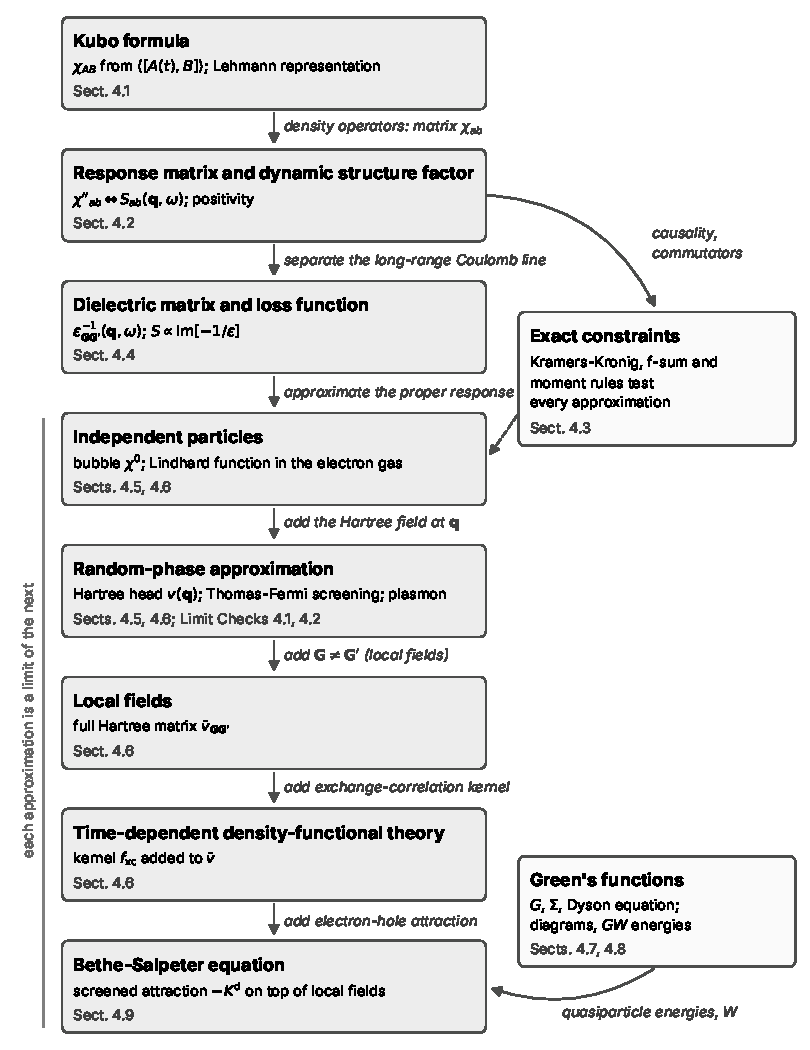
\includegraphics[width=0.85\linewidth]{figures/ch04/map04.pdf}
  \caption{The exact backbone and the hierarchy of approximations of the density response. The Kubo formula (\cref{sec:4.1}) leads to the response matrix and the dynamic structure factor (\cref{sec:4.2}); the exact constraints on both, the Kramers--Kronig relations and sum rules (\cref{sec:4.3}), hold in every approximation; separating the long-range Coulomb line gives the dielectric matrix and loss function (\cref{sec:4.4}). The approximations to the proper response add, in turn, the Hartree field at $\vect{q}$ (random-phase approximation, \cref{sec:4.5}, with Thomas--Fermi screening and the plasmon, \cref{lim:4.5a,lim:4.5b}), the local fields $\vect{G} \neq \vect{G}'$ and an exchange--correlation kernel (\cref{sec:4.6}), and the screened electron--hole attraction (\cref{sec:4.9}), with quasiparticle energies and the screened interaction $W$ from the Green's functions and diagrams of \cref{sec:4.7,sec:4.8}.}
  \label{fig:4-map}
\end{figure}

\section{The Kubo formula}\label{sec:4.1}

Apply to a crystal a weak potential that varies in space as a plane wave of wavevector $\vect{q}$ and in time at frequency $\omega$, and its electron density develops a ripple with the same wavevector and frequency. The amplitude of the ripple is proportional to the potential, and in general the ripple lags in phase. The ratio of ripple to potential is a response function. It is a property of the target alone, and it is fixed by correlations that the target has in equilibrium, before any potential is applied. The potential can be an applied electric field, a passing charge or the dark matter itself: between two of its plane-wave states, a dark-matter particle acts on the electrons through the density operator $n_e(\vect{q})$ (\cref{eq:2.3-nq}), the same operator through which a plane-wave potential acts. The treatment follows Refs.~\cite[Chap.~3]{giuliani2005quantum} and \cite[Chap.~6]{bruus2004many}.

\subsection{Response to a weak field}

The target has the Hamiltonian $H$, with all of its interactions, eigenstates $|i\rangle$ and energies $E_i$. Before the field acts, the target is in the Gibbs state $\op{\varrho} = \ee^{-\beta H}/\mathcal{Z}$ of \cref{eq:2.5-gibbs}. The field couples to a target operator $O_b$,
\begin{equation}
  H_{\mathrm{tot}}(t) = H + O_b\,\phi_{\mathrm{ext}}(t), \qquad \phi_{\mathrm{ext}}(t) \to 0 \ \text{ as } t \to -\infty ,
  \label{eq:4.1-Hext}
\end{equation}
where the external potential $\phi_{\mathrm{ext}}(t)$ is a number, not an operator: the source of the field is outside the target and is not changed by it. For a dimensionless $O_b$, such as a density, $\phi_{\mathrm{ext}}$ is an energy.

A real potential energy $\phi_{\mathrm{ext}}(t)\,\ee^{\ii\vect{q}\cdot\vect{r}} + \text{c.c.}$, acting on every electron, has exactly this form. Summed over electrons with \cref{eq:A.3-ne}, it is
\begin{equation*}
  \sum_j\bigl[\phi_{\mathrm{ext}}(t)\,\ee^{\ii\vect{q}\cdot\vect{r}_j} + \text{c.c.}\bigr] = n_e(\vect{q})\,\phi_{\mathrm{ext}}(t) + n_e(\vect{q})^\dagger\,\phi_{\mathrm{ext}}(t)^* ,
\end{equation*}
two terms of the form \cref{eq:4.1-Hext}, with $O_b = n_e(\vect{q})$ and $O_b = n_e(\vect{q})^\dagger$. To first order the responses to the two terms add, and we treat one at a time. The dark matter supplies one of them. Between its plane-wave states $\vect{p}$ and $\vect{p} - \vect{q}$ the interaction is $\tilde V(\vect{q})\,n_e(\vect{q})/\Vol$ (\cref{eq:A.3-vertex}): the term with $O_b = n_e(\vect{q})$, which gives the target the momentum $\vect{q}$.

The thermal state is a mixture, and each of its components obeys the Schr\"odinger equation with $H_{\mathrm{tot}}(t)$. The density matrix therefore evolves as $\ii\,\partial_t\op{\varrho}(t) = [H_{\mathrm{tot}}(t), \op{\varrho}(t)]$. As in \cref{sec:2.4}, we take the known part of the evolution out by going to the interaction picture, with one difference: the part we take out is the evolution under the full Hamiltonian $H$ of the target, interactions included, not under a free $H_0$. With $\op{\varrho}_{\mathrm{I}}(t) = \ee^{\ii Ht}\op{\varrho}(t)\,\ee^{-\ii Ht}$,
\begin{equation*}
  \ii\,\partial_t\op{\varrho}_{\mathrm{I}}(t) = \bigl[O_b(t)\,\phi_{\mathrm{ext}}(t),\,\op{\varrho}_{\mathrm{I}}(t)\bigr], \qquad O_b(t) = \ee^{\ii Ht}O_b\,\ee^{-\ii Ht} ,
\end{equation*}
the counterpart of \cref{eq:2.4-ipicture} for a density matrix. The Heisenberg operator $O_b(t)$ evolves under the target's own Hamiltonian, without the field. In the remote past $\op{\varrho}_{\mathrm{I}}$ is the Gibbs state, which commutes with $H$ and is unchanged by the transformation. Integrating once from $-\infty$ and keeping the term linear in $\phi_{\mathrm{ext}}$, the first-order term of the Dyson series \cref{eq:2.4-dyson}, gives
\begin{equation*}
  \op{\varrho}_{\mathrm{I}}(t) = \op{\varrho} - \ii\int_{-\infty}^{t}\dd t'\,\bigl[O_b(t'),\,\op{\varrho}\bigr]\,\phi_{\mathrm{ext}}(t') + O(\phi_{\mathrm{ext}}^2) .
\end{equation*}
The average of an operator $A$ at time $t$ is $\Tr[\op{\varrho}(t)A] = \Tr[\op{\varrho}_{\mathrm{I}}(t)A(t)]$, with $A(t)$ the Heisenberg operator. The zeroth-order term is the equilibrium average. In the first-order term the cyclic property of the trace moves $\op{\varrho}$ to the front, $\Tr([B, \op{\varrho}]A) = \Tr(\op{\varrho}[A, B])$, and the change of the average is
\begin{equation}
  \delta\langle A\rangle(t) = -\ii\int_{-\infty}^{t}\dd t'\,\bigl\langle[A(t),\,O_b(t')]\bigr\rangle\,\phi_{\mathrm{ext}}(t') ,
  \label{eq:4.1-general}
\end{equation}
with the average taken in the Gibbs state. The field at time $t'$ disturbs the target, the disturbance is carried to time $t$ by the target's own dynamics, and the commutator measures how much the disturbance shows up in $A$. Times $t' > t$ do not contribute. Since the Gibbs state is stationary, the commutator depends on $t - t'$ alone (\cref{sec:2.5}).

Which average responds to $O_b$? Suppose the target is invariant under translations, as the electron gas is. Then $O_b = n_e(\vect{q})$ adds the momentum $\vect{q}$ to every state it acts on, and the equilibrium average of $[A(t), O_b(t')]$ vanishes unless $A$ removes the same momentum. The operator that does so is the conjugate of an operator at $\vect{q}$, such as $n_e(\vect{q})^\dagger = n_e(-\vect{q})$. For the same reason the term with $n_e(\vect{q})^\dagger$ in the real potential above cannot change $\langle n_e(\vect{q})^\dagger\rangle$: both operators remove $\vect{q}$, and the average of their commutator would need the target to lose $2\vect{q}$. In a crystal, momentum is conserved only up to a reciprocal-lattice vector $\vect{G}$ (\cref{sec:3.1}). The field at $\vect{q}$ then also changes the averages at $\vect{q} + \vect{G}$, which are the local fields of \cref{sec:4.4}, and the two terms of a real potential mix only when $2\vect{q}$ is a reciprocal-lattice vector. Taking $A = O_a(\vect{q})^\dagger$ in \cref{eq:4.1-general} for a second target operator $O_a(\vect{q})$, with the Heisenberg operator $O_a(\vect{q},t)$ defined as $O_b(t)$, we arrive at the result.
\begin{keyresult}[Kubo formula]
\begin{equation}
  \begin{gathered}
  \delta\langle O_a(\vect{q})^\dagger\rangle(t) = \Vol\!\int_{-\infty}^{\infty}\dd t'\,R_{ab}(\vect{q}, t - t')\,\phi_{\mathrm{ext}}(t'), \\
  R_{ab}(\vect{q}, t) = -\frac{\ii}{\Vol}\,\Theta(t)\,\bigl\langle[O_a(\vect{q},t)^\dagger,\,O_b(\vect{q},0)]\bigr\rangle .
  \end{gathered}
  \label{eq:4.1-kubo}
\end{equation}
The change of $\langle O_a(\vect{q})^\dagger\rangle$, to first order in a field coupled as $O_b(\vect{q})\,\phi_{\mathrm{ext}}(t)$, is fixed by the commutator of the two operators in the unperturbed equilibrium state of the target.
\end{keyresult}
The step function $\Theta(t)$ imposes the restriction $t' < t$, and $R_{ab}$ is called the retarded response function. The equilibrium state enters through the average alone: the formula holds for any $H$, with any interactions, at any temperature. The factor $1/\Vol$ makes $R_{ab}$ intensive. For density operators the commutator is a sum over all the electrons and grows with the size of the target, and so does the induced $\delta\langle n_e(\vect{q})^\dagger\rangle$; their ratio to $\Vol$ does not. In a box, the inverse of \cref{eq:A.3-space} writes the electron density as $\Vol^{-1}\sum_{\vect{q}'}\ee^{-\ii\vect{q}'\cdot\vect{r}}n_e(\vect{q}')$, and the induced change of the density in position space is the ripple
\begin{equation*}
  \frac{1}{\Vol}\,\ee^{\ii\vect{q}\cdot\vect{r}}\,\delta\langle n_e(\vect{q})^\dagger\rangle(t) + \text{c.c.}
  = \ee^{\ii\vect{q}\cdot\vect{r}}\int\dd t'\,R_{ee}(\vect{q}, t - t')\,\phi_{\mathrm{ext}}(t') + \text{c.c.},
\end{equation*}
where $R_{ee}$ is the density response, with $O_a = O_b = n_e(\vect{q})$, in the labeling of \cref{app:A.7}. The response function is the induced density per unit applied potential energy, which is why $R_{ee}(\vect{q},\omega)$ has the dimension $\mathrm{eV}^3/\mathrm{eV} = \mathrm{eV}^2$; the function of time, $R_{ee}(\vect{q},t)$, has one power of energy more, $\mathrm{eV}^3$.

Kubo derived \cref{eq:4.1-general} in this generality~\cite{kubo1957statistical}, and it carries his name. Many texts write the response function as $\chi_{AB}$ and call it a susceptibility; others write $C^R_{AB}$. They usually omit the factor $1/\Vol$ and write the responding operator $A$ in place of our $O_a^\dagger$. A text that couples the field with a minus sign, $-O_b\,\phi_{\mathrm{ext}}$, has a response function of the opposite sign. In this book $\chi$ is the dark-matter particle and response functions are always $R$; \cref{app:B.2} lists the correspondence.

\subsection{Frequency dependence}

A field that oscillates at one frequency produces a response at the same frequency, with an amplitude set by the transform of $R_{ab}$. With the time convention of \cref{app:A.3}, the convolution in \cref{eq:4.1-kubo} becomes a product,
\begin{equation}
  \delta\langle O_a(\vect{q})^\dagger\rangle(\omega) = \Vol R_{ab}(\vect{q},\omega)\,\phi_{\mathrm{ext}}(\omega), \qquad
  R_{ab}(\vect{q},\omega) = -\frac{\ii}{\Vol}\int_0^\infty\dd t\;\ee^{\ii\omega t}\,\bigl\langle[O_a(\vect{q},t)^\dagger,\,O_b(\vect{q},0)]\bigr\rangle ,
  \label{eq:4.1-Romega}
\end{equation}
which is the definition \cref{eq:A.7-R}. For a target with a discrete spectrum the commutator oscillates forever, and the integral needs a prescription to converge, which the switching supplies. Turn the field on slowly, $\phi_{\mathrm{ext}}(t) = \phi_0\,\ee^{-\ii\omega t + \eta_{\mathrm{b}}t}$ with a small rate $\eta_{\mathrm{b}} > 0$. Substituting $s = t - t'$ in \cref{eq:4.1-kubo},
\begin{equation*}
  \delta\langle O_a(\vect{q})^\dagger\rangle(t) = \Vol\phi_{\mathrm{ext}}(t)\int_0^\infty\dd s\;\ee^{\ii(\omega + \ii\eta_{\mathrm{b}})s}\,R_{ab}(\vect{q},s) .
\end{equation*}
The response follows the field, and its amplitude is the transform of $R_{ab}$ at the complex frequency $\omega + \ii\eta_{\mathrm{b}}$. The physical response function is the limit $\eta_{\mathrm{b}} \to 0^+$, and $\omega$ in \cref{eq:4.1-Romega} always stands for $\omega + \ii0^+$. This is the adiabatic switching of \cref{sec:2.4}, which put $+\ii0^+$ into the energy denominators there.

For operators with $O(-\vect{q}) = O(\vect{q})^\dagger$, the response at $-\vect{q}$ is the complex conjugate of the response at $\vect{q}$. Since $\langle X\rangle^* = \langle X^\dagger\rangle$ and $[A, B]^\dagger = -[A^\dagger, B^\dagger]$, the complex conjugate of $R_{ab}(\vect{q},t)$ is $-(\ii/\Vol)\,\Theta(t)\,\langle[O_a(\vect{q},t), O_b(\vect{q})^\dagger]\rangle$. For densities and other operators with this property, it is the response at $-\vect{q}$:
\begin{equation}
  R_{ab}(\vect{q},t)^* = R_{ab}(-\vect{q},t), \qquad R_{ab}(\vect{q},\omega)^* = R_{ab}(-\vect{q},-\omega) \quad (\omega \text{ real}) .
  \label{eq:4.1-reality}
\end{equation}
It is what makes the ripple produced by a real potential a real function of $\vect{r}$ and $t$. In a target with inversion or time-reversal symmetry, where $R_{ee}(-\vect{q},\omega) = R_{ee}(\vect{q},\omega)$, the real part of the density response is even in $\omega$ and its imaginary part odd.

\subsection{Lehmann representation}

In the eigenstates of $H$ every Heisenberg operator oscillates at the energies of the transitions it causes, $\langle i|O(t)|f\rangle = \ee^{\ii(E_i - E_f)t}\langle i|O|f\rangle$, and the commutator in \cref{eq:4.1-Romega} becomes a sum of such oscillations. Writing out its two products, with the Gibbs weights $p_i = \ee^{-\beta E_i}/\mathcal{Z}$, and inserting a complete set of states $|f\rangle$ between the operators,
\begin{equation*}
  \bigl\langle[O_a(\vect{q},t)^\dagger, O_b(\vect{q})]\bigr\rangle = \sum_{i,f}p_i\Bigl[\langle i|O_a^\dagger|f\rangle\langle f|O_b|i\rangle\,\ee^{-\ii(E_f - E_i)t} - \langle i|O_b|f\rangle\langle f|O_a^\dagger|i\rangle\,\ee^{+\ii(E_f - E_i)t}\Bigr] ,
\end{equation*}
where the operators without a time argument are taken at $t = 0$ and we drop the argument $\vect{q}$. The time integral of each oscillation, with $\omega + \ii0^+$, is elementary, $-\ii\int_0^\infty\dd t\,\ee^{\ii(\omega \mp (E_f - E_i) + \ii0^+)t} = 1/[\omega \mp (E_f - E_i) + \ii0^+]$.
\begin{keyresult}[Lehmann representation]
\begin{equation}
  R_{ab}(\vect{q},\omega) = \frac{1}{\Vol}\sum_{i,f}p_i\left[\frac{\langle i|O_a^\dagger|f\rangle\langle f|O_b|i\rangle}{\omega - (E_f - E_i) + \ii0^+} - \frac{\langle i|O_b|f\rangle\langle f|O_a^\dagger|i\rangle}{\omega + (E_f - E_i) + \ii0^+}\right] .
  \label{eq:4.1-lehmann}
\end{equation}
The response is a sum of simple poles at the transition energies of the target, each displaced by $-\ii0^+$ below the real axis and weighted by the thermal population of its initial state and a product of matrix elements.
\end{keyresult}
This is \cref{eq:A.7-lehmann}. The term with the pole at $\omega = E_f - E_i$ is what the optics literature calls the resonant term, and the one with the pole at $\omega = -(E_f - E_i)$ the antiresonant term. For a target in its ground state, $E_f - E_i \ge 0$, and the resonant term has its poles at positive $\omega$. The interactions of the target, however strong, enter through the exact energies and matrix elements. No approximation has been made beyond first order in $\phi_{\mathrm{ext}}$.

The poles split the response into two parts with different meanings. By the Sokhotski--Plemelj formula \cref{eq:2.4-SP} (\cref{app:C.4}), each denominator is a principal value minus $\ii\pi$ times a delta function. The principal value collects transitions that the field drives off resonance. They are never completed, they shift the target's energy, and they make the target polarizable, as the off-shell intermediate states of \cref{sec:2.4} did. The delta functions collect the transitions that conserve energy, and they make up the imaginary part. For a diagonal element, $a = b$, the weights are squared matrix elements, $|\langle f|O_a|i\rangle|^2$ in the resonant term and $|\langle f|O_a^\dagger|i\rangle|^2$ in the antiresonant one. The imaginary part is then a difference of two transition sums \cref{eq:2.5-transum}:
\begin{equation}
  \Imag R_{aa}(\vect{q},\omega) = -\frac{\pi}{\Vol}\Bigl[\mathcal{S}_{O_a}(\omega) - \mathcal{S}_{O_a^\dagger}(-\omega)\Bigr] .
  \label{eq:4.1-ImR}
\end{equation}
The transition sum $\mathcal{S}_{O_a}(\omega)$ counts the transitions in which the target takes the energy $\omega$; $\mathcal{S}_{O_a^\dagger}(-\omega)$ counts those in which it gives up $\omega$. At $T = 0$ the target starts in its ground state, nothing can give up energy, and $\Imag R_{aa} < 0$ for $\omega > 0$. At finite temperature both sums contribute, and detailed balance \cref{eq:2.5-db} makes $\mathcal{S}_{O_a}(\omega)$ larger by the factor $\ee^{\beta\omega}$. \Cref{sec:4.2} turns this into the fluctuation--dissipation theorem, which ties $\Imag R_{aa}$ to the dynamic structure factor.

\paragraph{Absorbed power.} The sign of $\Imag R$ is the statement that a target in equilibrium absorbs energy from a field. Take a Hermitian $O_b$, so that $R_{bb}(t)$ is real (the average of the commutator of two Hermitian operators is imaginary), and a real field $\phi_{\mathrm{ext}}(t) = \phi_0\cos\omega t$ with $\omega > 0$. The field does work on the target at the rate $\langle\partial H_{\mathrm{tot}}/\partial t\rangle = \langle O_b\rangle(t)\,\dot\phi_{\mathrm{ext}}(t)$. The field has components $\tfrac12\phi_0$ at the frequencies $\pm\omega$, and by \cref{eq:4.1-Romega} the induced $\delta\langle O_b\rangle$ has components $\tfrac12\phi_0\Vol R_{bb}(\pm\omega)$, with $R_{bb}(-\omega) = R_{bb}(\omega)^*$ since $R_{bb}(t)$ is real. In the time average of the product the cross terms between $+\omega$ and $-\omega$ alone survive, and the mean absorbed power is
\begin{equation}
  P = -\frac{\omega\,\phi_0^2}{2}\,\Vol\,\Imag R_{bb}(\omega) = \frac{\pi}{2}\,\omega\,\phi_0^2\,\Bigl[\mathcal{S}_{O_b}(\omega) - \mathcal{S}_{O_b}(-\omega)\Bigr] ,
  \label{eq:4.1-power}
\end{equation}
where the expression in transition sums follows from \cref{eq:4.1-ImR}. This is $\omega$ times the difference of the absorption and emission rates of the golden rule for a harmonic perturbation, \cref{eq:2.1-harmonic} with $\op{O} = \tfrac12\phi_0O_b$, averaged over the thermal state as in \cref{sec:2.5}. The imaginary part of a diagonal response is therefore its dissipative part. The same formula describes a bosonic dark-matter field that couples to $O_b$. With $\omega = m_\phi$, the amplitude $\phi_0$ is then the field amplitude of \cref{sec:2.1}, $\phi_0^2 = 2\rho_\chi/m_\phi^2$, times the coupling constant of the field to $O_b$, which we set to one here. Then $P/m_\phi$ is the rate at which the field is absorbed in the volume $\Vol$, which is why absorption rates are proportional to $-\Imag R$ (\cref{chap:8}).

\paragraph{Static limit.} At $\omega \to 0$ the Lehmann form measures how much the target deforms in a static field. For a Hermitian $O_b$ the resonant and antiresonant terms of a pair $i, f$ have the same weight, so pairs with $E_f = E_i$ cancel, and the rest add:
\begin{equation*}
  \Vol R_{bb}(0) = -2\sum_{i,f}p_i\,\frac{|\langle f|O_b|i\rangle|^2}{E_f - E_i} \qquad (E_f \neq E_i) .
\end{equation*}
At $T = 0$ every term is negative. Compare second-order perturbation theory for a static $H_{\mathrm{ext}} = O_b\phi_0$: the ground-state energy is shifted by $-\phi_0^2\sum_f|\langle f|O_b|0\rangle|^2/(E_f - E_0)$, which is $\tfrac12\Vol R_{bb}(0)\,\phi_0^2$. A static response is negative because the target always lowers its energy by yielding to a static field; for the density, electrons leave the regions where the potential energy is high. At finite temperature the limit $\omega \to 0$ describes a target that is deformed by a slowly applied field while isolated from any bath, Kubo's isolated response. The isothermal response, in which the target stays in equilibrium with a bath, has an extra term proportional to $\beta$ from matrix elements of $O_b$ between states of equal energy; the two agree when there are none~\cite{kubo1957statistical}.

\begin{workedexample}{The driven harmonic oscillator}\label{we:4-oscillator}
Take one mode of frequency $\omega_0$, $H = \omega_0 d^\dagger d$, and the operator $O_a = O_b = \lambda_{\mathrm{osc}}(d + d^\dagger)$ of \cref{we:2-oscillator}, with $\lambda_{\mathrm{osc}}$ real. A single oscillator has no volume of its own, and the combination $\Vol R$ is its response, independent of the box. The Heisenberg operators follow from the commutator $[d, H] = \omega_0 d$, which integrates, as for the fermion operators of \cref{sec:2.3}, to $d(t) = d\,\ee^{-\ii\omega_0t}$. The commutator in \cref{eq:4.1-kubo} is then a number,
\begin{equation*}
  [O(t), O] = \lambda_{\mathrm{osc}}^2\bigl([d, d^\dagger]\,\ee^{-\ii\omega_0t} + [d^\dagger, d]\,\ee^{\ii\omega_0t}\bigr) = -2\ii\lambda_{\mathrm{osc}}^2\sin\omega_0t ,
\end{equation*}
the same in every state, and $\Vol R(t) = -2\lambda_{\mathrm{osc}}^2\,\Theta(t)\sin\omega_0t$. With $\int_0^\infty\dd t\,\ee^{\ii zt}\sin\omega_0t = \omega_0/(\omega_0^2 - z^2)$ for $\Imag z > 0$, its transform is
\begin{equation}
  \Vol R(\omega) = \frac{2\lambda_{\mathrm{osc}}^2\omega_0}{(\omega + \ii0^+)^2 - \omega_0^2} = \lambda_{\mathrm{osc}}^2\left[\frac{1}{\omega - \omega_0 + \ii0^+} - \frac{1}{\omega + \omega_0 + \ii0^+}\right] .
  \label{eq:4.1-osc}
\end{equation}
The Lehmann form gives the same. From the level $n$, $O$ reaches $n + 1$ with $|\langle n+1|O|n\rangle|^2 = \lambda_{\mathrm{osc}}^2(n + 1)$ and $n - 1$ with $\lambda_{\mathrm{osc}}^2 n$, and averaged with the thermal weights of \cref{eq:2.5-nF} the resonant term of \cref{eq:4.1-lehmann} is $\lambda_{\mathrm{osc}}^2[(n_{\mathrm{B}}(\omega_0) + 1)/(\omega - \omega_0) + n_{\mathrm{B}}(\omega_0)/(\omega + \omega_0)]$, with $n_{\mathrm{B}}(\omega_0)$ the Bose occupation of the mode. The antiresonant term has the same weights with the denominators exchanged. Their difference is \cref{eq:4.1-osc}, and $n_{\mathrm{B}}(\omega_0)$ cancels. The oscillator absorbs and emits more often at higher temperature, by the factors $n_{\mathrm{B}}(\omega_0) + 1$ and $n_{\mathrm{B}}(\omega_0)$ of \cref{we:2-oscillator}, but the net response to a field is independent of temperature.

The reason is that the oscillator is a linear system, and the quantum response is the classical one. For a particle of mass $M_{\mathrm{osc}}$ in a harmonic well, the displacement is $x = (2M_{\mathrm{osc}}\omega_0)^{-1/2}(d + d^\dagger)$, so $O = x$ has $\lambda_{\mathrm{osc}}^2 = 1/(2M_{\mathrm{osc}}\omega_0)$. The field $H_{\mathrm{ext}} = x\,\phi_{\mathrm{ext}}$ is a force $-\phi_{\mathrm{ext}}$, and Newton's equation $M_{\mathrm{osc}}(\ddot x + \omega_0^2x) = -\phi_{\mathrm{ext}}$, with $x \propto \ee^{-\ii\omega t}$, gives $x(\omega) = \phi_{\mathrm{ext}}(\omega)/[M_{\mathrm{osc}}(\omega^2 - \omega_0^2)]$, which is \cref{eq:4.1-osc} with this $\lambda_{\mathrm{osc}}$. The static limit is the stretched spring, $x = -\phi_{\mathrm{ext}}/(M_{\mathrm{osc}}\omega_0^2)$, and $\Vol R(0) = -2\lambda_{\mathrm{osc}}^2/\omega_0$; the energy $\tfrac12\Vol R(0)\phi_0^2 = -\lambda_{\mathrm{osc}}^2\phi_0^2/\omega_0$ is the second-order shift of the ground state by $\lambda_{\mathrm{osc}}\phi_0(d + d^\dagger)$, as the static limit above requires.

A real oscillator also loses energy, to other modes or to electrons. With a damping term $M_{\mathrm{osc}}\varGamma_{\mathrm{w}}\dot x$ added to Newton's equation, where $\varGamma_{\mathrm{w}}$ is the rate at which the energy of the free oscillation decays, the response becomes
\begin{equation*}
  \Vol R(\omega) = \frac{2\lambda_{\mathrm{osc}}^2\omega_0}{\omega^2 + \ii\varGamma_{\mathrm{w}}\omega - \omega_0^2}, \qquad
  -\Imag\Vol R(\omega) = \frac{2\lambda_{\mathrm{osc}}^2\omega_0\,\varGamma_{\mathrm{w}}\omega}{(\omega^2 - \omega_0^2)^2 + \varGamma_{\mathrm{w}}^2\omega^2} .
\end{equation*}
The infinitesimal $0^+$ has become the finite width $\varGamma_{\mathrm{w}}$, as in \cref{eq:2.4-width}. The absorptive part $-\Imag\Vol R$ is a resonance of height $2\lambda_{\mathrm{osc}}^2/\varGamma_{\mathrm{w}}$ at $\omega = \omega_0$, ten times $\lambda_{\mathrm{osc}}^2/\omega_0$ for $\varGamma_{\mathrm{w}} = 0.2\,\omega_0$, and it is positive at every $\omega > 0$ (\cref{fig:4-poles}b). The real part is negative below the resonance, where the oscillator follows the force in phase, and positive above it, where it moves against the force. At large $\omega$ it falls as $2\lambda_{\mathrm{osc}}^2\omega_0/\omega^2$.
\end{workedexample}

\subsection{Causality and analyticity}

A response cannot precede its cause. In \cref{eq:4.1-kubo} this is the step function $\Theta(t)$, and in frequency it becomes a statement about complex $\omega$. Define the transform at a complex frequency $z$,
\begin{equation}
  R_{ab}(\vect{q},z) = \int_0^\infty\dd t\;\ee^{\ii zt}\,R_{ab}(\vect{q},t) .
  \label{eq:4.1-Rz}
\end{equation}
For $\Imag z > 0$ the factor $\ee^{\ii zt} = \ee^{\ii t\Real z}\ee^{-t\Imag z}$ decays, while $R_{ab}(\vect{q},t)$ stays bounded: in a stable target all energies are real, and the commutator average oscillates without growing. The integral then converges, it may be differentiated under the integral sign with respect to $z$, and $R_{ab}(\vect{q},z)$ is analytic everywhere in the upper half plane. This used causality, which restricts the integral to $t > 0$, and stability, which keeps $R_{ab}(\vect{q},t)$ from growing. The physical response is the boundary value on the real axis approached from above, $R_{ab}(\vect{q},\omega + \ii0^+)$, which is the prescription found from the switching. For $\Imag z < 0$ the integral diverges, and the response there is defined, if at all, by analytic continuation. \Cref{app:C.5} states these results in general.

The Lehmann form shows the same thing pole by pole. With $\omega + \ii0^+$ replaced by $z$, \cref{eq:4.1-lehmann} is a sum of terms $1/[z \mp (E_f - E_i)]$, whose poles lie on the real axis, and the physical frequency passes just above them (\cref{fig:4-poles}a). In a finite target the poles are isolated, and the imaginary part on the real axis is a comb of delta functions. In a macroscopic target the transition energies crowd together, with spacings that shrink as the volume grows. If the limit $\Vol \to \infty$ is taken first, at a fixed small $\eta_{\mathrm{b}}$, the sums over $f$ become integrals, and $R_{ab}(\vect{q},\omega + \ii\eta_{\mathrm{b}})$ tends to a smooth function as $\eta_{\mathrm{b}} \to 0^+$. The poles have merged into a branch cut along the parts of the real axis where the spectrum is continuous. The opposite order of limits returns the comb. This is the time window of the golden rule (\cref{sec:2.1}) once more. The switching rate $\eta_{\mathrm{b}}$ must be small compared with the scale on which the response varies, and large compared with the level spacing, which a macroscopic target makes arbitrarily small.

Across the cut, the continuation of $R_{ab}$ into the lower half plane can have poles at complex frequencies. They are resonances, long-lived collective or single-particle excitations. A pole at $z_{\mathrm{p}}$ contributes $\ee^{-\ii z_{\mathrm{p}}t}$ to $R_{ab}(\vect{q},t)$, which decays only if $\Imag z_{\mathrm{p}} < 0$. The damped oscillator of \cref{we:4-oscillator} shows them in closed form. Its response has poles where $\omega^2 + \ii\varGamma_{\mathrm{w}}\omega - \omega_0^2 = 0$,
\begin{equation*}
  \omega = -\frac{\ii\varGamma_{\mathrm{w}}}{2} \pm \Bigl(\omega_0^2 - \frac{\varGamma_{\mathrm{w}}^2}{4}\Bigr)^{1/2} .
\end{equation*}
For $\varGamma_{\mathrm{w}} < 2\omega_0$ they lie on the circle $|\omega| = \omega_0$ in the lower half plane, at a depth $\varGamma_{\mathrm{w}}/2$ that is the decay rate of the amplitude. At critical damping, $\varGamma_{\mathrm{w}} = 2\omega_0$, they meet at $-\ii\omega_0$, and for larger $\varGamma_{\mathrm{w}}$ they move apart along the negative imaginary axis. For no positive $\varGamma_{\mathrm{w}}$ do they cross into the upper half plane, where a pole would describe a response that grows exponentially after the field is gone. The plasmon (\cref{sec:4.5}) and the quasiparticles of \cref{sec:4.7} are poles of this kind.

\begin{figure}[tbp]
  \centering
  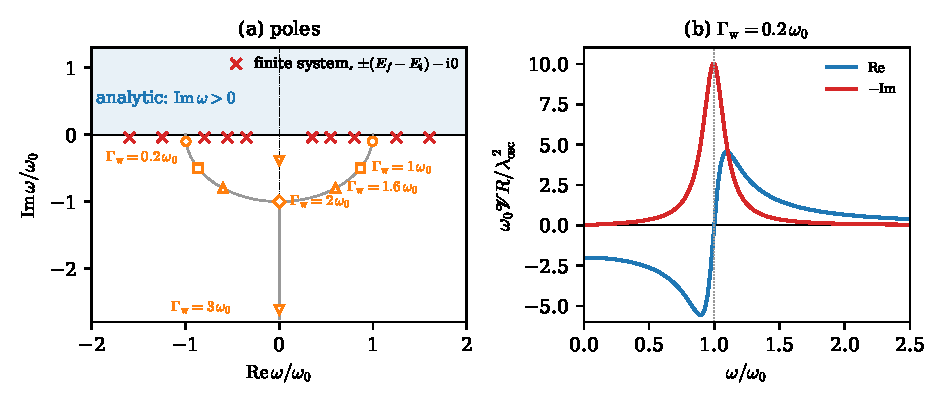
\includegraphics[width=\linewidth]{figures/ch04/fig4_1.pdf}
  \caption{Poles of the retarded response function in the complex frequency plane $\omega$, in units of an oscillator frequency $\omega_0$. (a) The response is analytic in the upper half plane (shaded). A finite target has poles at its transition energies $\pm(E_f - E_i)$, displaced by an infinitesimal $-\ii0$ below the real axis (crosses, at illustrative transition energies). A harmonic oscillator with energy damping rate $\varGamma_{\mathrm{w}}$ has poles at $-\ii\varGamma_{\mathrm{w}}/2 \pm (\omega_0^2 - \varGamma_{\mathrm{w}}^2/4)^{1/2}$ (open symbols, for the values of $\varGamma_{\mathrm{w}}$ marked). They lie on the circle $|\omega| = \omega_0$ below critical damping, $\varGamma_{\mathrm{w}} = 2\omega_0$, and on the negative imaginary axis above it; for $\varGamma_{\mathrm{w}} = 3\omega_0$ the upper of the two is at $-0.38\,\ii\omega_0$. (b) Real part and minus the imaginary part of $\Vol R$ for the damped oscillator with $\varGamma_{\mathrm{w}} = 0.2\,\omega_0$ and coupling $\lambda_{\mathrm{osc}}(d + d^\dagger)$, on the real axis. The absorptive part peaks at $2\lambda_{\mathrm{osc}}^2/\varGamma_{\mathrm{w}}$ at $\omega = \omega_0$; the real part is negative below the resonance and positive above it, and tends to $-2\lambda_{\mathrm{osc}}^2/\omega_0$ at $\omega = 0$.}
  \label{fig:4-poles}
\end{figure}

How fast $R_{ab}$ falls at large $|z|$ follows from the Lehmann form too. Expanding $1/[z \mp (E_f - E_i)] = 1/z \pm (E_f - E_i)/z^2 + \dots$ in \cref{eq:4.1-lehmann}, the coefficient of $1/z$ is the equal-time commutator, and in the coefficient of $1/z^2$ the resonant and antiresonant terms combine into a double commutator:
\begin{equation}
  R_{ab}(\vect{q},z) = \frac{\langle[O_a^\dagger, O_b]\rangle}{\Vol z} + \frac{\langle[O_a^\dagger, [H, O_b]]\rangle}{\Vol z^2} + O(z^{-3}) .
  \label{eq:4.1-tail}
\end{equation}
The coefficient of $1/z^2$ is checked by writing out $\langle i|O_a^\dagger HO_b - O_a^\dagger O_bH - HO_bO_a^\dagger + O_bHO_a^\dagger|i\rangle$ in eigenstates, which gives $\sum_f(E_f - E_i)\bigl[\langle i|O_a^\dagger|f\rangle\langle f|O_b|i\rangle + \langle i|O_b|f\rangle\langle f|O_a^\dagger|i\rangle\bigr]$. Density operators at different wavevectors commute, since both are functions of the electron positions alone, and the density response therefore falls as $1/z^2$. When the potential acting on the electrons is local, only the kinetic energy contributes to the coefficient, and the result, the f-sum rule of \cref{sec:4.3}, depends only on the electron density. For the oscillator, $[O, [H, O]] = 2\lambda_{\mathrm{osc}}^2\omega_0$, the coefficient found in \cref{we:4-oscillator}. Analyticity in the upper half plane together with this decay leads to the Kramers--Kronig relations, which reconstruct the real part of $R_{ab}$ on the real axis from its imaginary part (\cref{sec:4.3}).

\begin{workedexample}{The two-level system}\label{we:4-twolevel}
Take the two-level system of \cref{sec:2.5}: states $|0\rangle$ and $|1\rangle$ with splitting $\Delta_{\mathrm{tl}}$, Gibbs weights $p_0$ and $p_1$, and a Hermitian operator $O_a = O_b = O$ with only the off-diagonal element $O_{10} = \langle 1|O|0\rangle$. The Lehmann form \cref{eq:4.1-lehmann} has four entries. In the resonant term, $i = 0$ contributes $p_0|O_{10}|^2/(\omega - \Delta_{\mathrm{tl}})$ and $i = 1$ contributes $p_1|O_{10}|^2/(\omega + \Delta_{\mathrm{tl}})$. In the antiresonant term the same weights appear with the poles exchanged and a minus sign. Altogether,
\begin{equation}
  \Vol R(\omega) = (p_0 - p_1)\,|O_{10}|^2\left[\frac{1}{\omega - \Delta_{\mathrm{tl}} + \ii0^+} - \frac{1}{\omega + \Delta_{\mathrm{tl}} + \ii0^+}\right]
  = \frac{2\Delta_{\mathrm{tl}}\,|O_{10}|^2\tanh(\beta\Delta_{\mathrm{tl}}/2)}{(\omega + \ii0^+)^2 - \Delta_{\mathrm{tl}}^2} ,
  \label{eq:4.1-twolevel}
\end{equation}
with $p_0 - p_1 = \tanh(\beta\Delta_{\mathrm{tl}}/2)$ from \cref{eq:2.5-gibbs}. It has the form of the oscillator, \cref{eq:4.1-osc}, with $\omega_0 \to \Delta_{\mathrm{tl}}$ and $\lambda_{\mathrm{osc}}^2 \to (p_0 - p_1)|O_{10}|^2$, but now the temperature matters. At $T = \Delta_{\mathrm{tl}}/2$ the weights are 0.881 and 0.119 (\cref{fig:2-twolevel}), the response is reduced by the factor 0.762, and $\Vol R(0) = -1.523\,|O_{10}|^2/\Delta_{\mathrm{tl}}$. At $T \gg \Delta_{\mathrm{tl}}$, $\tanh(\beta\Delta_{\mathrm{tl}}/2) \to \Delta_{\mathrm{tl}}/2T$ and $\Vol R(0) \to -|O_{10}|^2/T$. For a spin $\tfrac12$ in a magnetic field, with $\Delta_{\mathrm{tl}}$ the Zeeman splitting and $O$ a transverse component of its magnetic moment, this is the Curie law of a paramagnet: the static susceptibility falls as $1/T$.

The temperature dependence comes from the weight $p_0 - p_1$. The field drives the upward transition from $|0\rangle$ and stimulated emission from $|1\rangle$ with the same matrix element, so the excited population cancels part of the absorption, and the absorbed power \cref{eq:4.1-power} is proportional to $p_0 - p_1$. Since $p_1 < p_0$ at every temperature (\cref{sec:2.5}), a two-level system in equilibrium always absorbs, and becomes transparent only as $T \to \infty$. The oscillator escapes this saturation because its matrix elements grow up the ladder: the extra absorption from level $n$, weighted by $n + 1$, exactly compensates the emission, weighted by $n$, which is why $n_{\mathrm{B}}(\omega_0)$ dropped out of \cref{eq:4.1-osc}. The tail coefficient of \cref{eq:4.1-tail} is $\langle[O, [H, O]]\rangle = 2\Delta_{\mathrm{tl}}(p_0 - p_1)|O_{10}|^2$, temperature dependent here and constant for the oscillator.

The two examples also mark where linear response stops. For the oscillator, the commutator $[O(t), O(t')]$ is a number, every nested commutator of higher order vanishes, and with it every higher-order term of the Dyson series, so \cref{eq:4.1-osc} holds at any field strength. The two-level system saturates. On resonance the field moves population between $|0\rangle$ and $|1\rangle$, and \cref{eq:4.1-twolevel} holds only while that transfer is small: the drive $|O_{10}\phi_0|$ must be small compared with the width of the transition, the weak-drive condition of \cref{app:D.3}. A stronger field makes the populations oscillate at the Rabi frequency, a response that is not linear in the field.
\end{workedexample}

\section{Correlations and the dynamic structure factor}\label{sec:4.2}

A dark-matter particle in silicon scatters at a rate fixed by the dynamic structure factor $S(\vect{q},\omega)$ of \cref{eq:2.5-golden}, which counts the transitions the target makes. A weak potential applied from outside, acting through the same density operator (\cref{sec:4.1}), makes the density ripple by an amount fixed by the response function $R_{ee}$ of \cref{eq:4.1-kubo}. Both are built from the same matrix elements and the same Gibbs weights, and we will see that at each $\vect{q}$ and $\omega$ either one fixes the other. This is the fluctuation--dissipation theorem, and it lets every method that computes a response also compute a rate. Before we get there, we look at $S$ from two other sides. In space and time it is the Fourier transform of a density--density correlation function, Van Hove's picture of a scattering experiment. Over several target operators it is a positive matrix, which keeps every rate positive and bounds the interference between two couplings. We end with independent particles, for which $S$ has a closed form in the electron gas, and the hydrogen atom of \cref{sec:2.2} comes back as a special case. The treatment follows Refs.~\cite[Chaps.~3 and 4]{giuliani2005quantum} and \cite[Chap.~2]{pines1966theory}.

\subsection{The response matrix}

A dark photon couples to the charge of the electrons and of the nuclei, with opposite signs, and other mediators couple to spin or to the nucleon number (\cref{sec:1.4}). In general the interaction between the dark-matter plane waves $\vect{p}$ and $\vect{p} - \vect{q}$ is a sum $\Vol^{-1}\sum_b\tilde V_b(\vect{q})\,O_b(\vect{q})$ over target operators $O_b(\vect{q})$, each with its own potential $\tilde V_b(\vect{q})$; the density coupling of \cref{eq:A.3-vertex} is the case of a single term, $O_e = n_e(\vect{q})$ with $\tilde V_e = \tilde V$. The golden-rule amplitude to reach $|f\rangle$ from $|i\rangle$ is then $\Vol^{-1}\sum_b\tilde V_b\langle f|O_b|i\rangle$. Its square has cross terms $\tilde V_a^*\tilde V_b\,\langle i|O_a^\dagger|f\rangle\langle f|O_b|i\rangle$, and the target enters through the matrix of their thermal sums.
\begin{keyresult}[Response matrix]
\begin{equation}
  \begin{aligned}
  S_{ab}(\vect{q},\omega) &= \frac{2\pi}{\Vol}\sum_{i,f}p_i\,\langle i|O_a(\vect{q})^\dagger|f\rangle\langle f|O_b(\vect{q})|i\rangle\,\delta(\omega - E_f + E_i) \\
  &= \frac{1}{\Vol}\int_{-\infty}^{\infty}\dd t\;\ee^{\ii\omega t}\,\bigl\langle O_a(\vect{q},t)^\dagger\,O_b(\vect{q},0)\bigr\rangle .
  \end{aligned}
  \label{eq:4.2-Sab}
\end{equation}
Its diagonal elements are the transition sums of \cref{eq:2.5-transum}, $S_{aa} = (2\pi/\Vol)\,\mathcal{S}_{O_a}$, and the dynamic structure factor is the density element, $S \equiv S_{ee}$.
\end{keyresult}
The correlation-function form follows as \cref{eq:2.5-corr} did. Inserting a complete set of states between the two operators, each term oscillates as $\ee^{-\ii(E_f - E_i)t}$, and the time integral turns the oscillation into $2\pi\,\delta(\omega - E_f + E_i)$. This is the definition \cref{eq:A.7-S}, and its density element is $S(\vect{q},\omega)$ of \cref{eq:2.5-golden}, Ref.~\cite[Eq.~(4)]{knapen2021dark}, with the same normalization. Exchanging $a$ and $b$ complex-conjugates each term, so $S_{ab}^* = S_{ba}$ and the matrix is Hermitian. Like $R_{ab}$, it is intensive, and for density operators it has the dimension $\mathrm{eV}^2$. Detailed balance carries over with the indices exchanged. For operators with $O(-\vect{q}) = O(\vect{q})^\dagger$, relabeling $i \leftrightarrow f$ as in \cref{eq:2.5-db} gives $S_{ab}(-\vect{q},-\omega) = \ee^{-\beta\omega}S_{ba}(\vect{q},\omega)$, which is \cref{eq:A.7-DB}.

The sum over final dark-matter momenta is the one of \cref{sec:2.5}, term by term, and the rate per dark-matter particle is
\begin{equation}
  \varGamma = \int\frac{\dd^3q}{(2\pi)^3}\sum_{a,b}\tilde V_a(\vect{q})^*\,\tilde V_b(\vect{q})\,S_{ab}(\vect{q},\omega_{\vect{q}}) ,
  \label{eq:4.2-rate}
\end{equation}
with $\omega_{\vect{q}}$ the energy deposited at $\vect{q}$ (\cref{sec:2.5}). For a single operator it reduces to $\int\dd^3q\,(2\pi)^{-3}|\tilde V_a|^2S_{aa}$, and for the density to \cref{eq:2.5-golden}. The off-diagonal elements carry the interference between two couplings. For a dark photon, for instance, the electron and nuclear densities enter with potentials of opposite sign, and $S_{ab}$ between them measures how the electrons follow a recoiling nucleus; \cref{chap:8} builds the general rate on \cref{eq:4.2-rate}.

\subsection{Correlations in space and time}

At a typical momentum transfer $q_0 = \alpha m_e = \SI{3.73}{keV}$ the dark matter probes the electron density on a length $2\pi/q_0 = \SI{3.32}{\angstrom}$, and at an energy of \SI{10}{eV} over a time $1/\omega = \SI{0.066}{fs}$. The structure factor can be read as a statement about the density on these scales. Van Hove introduced this reading for neutron scattering~\cite{vanhove1954correlations}: the rate measures how the density at one place and time is correlated with the density at another. To see it, write the density in position space, $\op{\nd}_e(\vect{r}) = \sum_j\delta^3(\vect{r} - \vect{r}_j)$, the operator whose transform \cref{eq:A.3-space} is $n_e(\vect{q})$, and define the Van Hove correlation function
\begin{equation}
  \mathcal{G}_{\mathrm{VH}}(\vect{r},t) = \frac{1}{N_e}\int\dd^3r'\,\bigl\langle\op{\nd}_e(\vect{r}',0)\,\op{\nd}_e(\vect{r}' + \vect{r},t)\bigr\rangle ,
  \label{eq:4.2-GVH}
\end{equation}
with $N_e$ the number of electrons in the volume $\Vol$ and the Heisenberg operators of \cref{sec:4.1}. In the correlation form \cref{eq:4.2-Sab}, stationarity moves the time from one operator to the other, $\langle n_e(\vect{q},t)^\dagger n_e(\vect{q},0)\rangle = \langle n_e(\vect{q},0)^\dagger n_e(\vect{q},-t)\rangle$. Writing both operators as integrals over position, $n_e(\vect{q})^\dagger = \int\dd^3r'\,\ee^{-\ii\vect{q}\cdot\vect{r}'}\op{\nd}_e(\vect{r}')$, and writing the position in $n_e(\vect{q},-t)$ as $\vect{r}' + \vect{r}$,
\begin{equation*}
  \begin{aligned}
  \langle n_e(\vect{q},0)^\dagger n_e(\vect{q},-t)\rangle &= \int\dd^3r\;\ee^{\ii\vect{q}\cdot\vect{r}}\int\dd^3r'\,\bigl\langle\op{\nd}_e(\vect{r}',0)\,\op{\nd}_e(\vect{r}'+\vect{r},-t)\bigr\rangle \\
  &= N_e\int\dd^3r\;\ee^{\ii\vect{q}\cdot\vect{r}}\,\mathcal{G}_{\mathrm{VH}}(\vect{r},-t) .
  \end{aligned}
\end{equation*}
Dividing by $\Vol$, integrating over $t$ with $\ee^{\ii\omega t}$ and reversing the sign of $t$,
\begin{equation}
  S(\vect{q},\omega) = \nd_e\int_{-\infty}^{\infty}\dd t\int\dd^3r\;\ee^{\ii(\vect{q}\cdot\vect{r} - \omega t)}\,\mathcal{G}_{\mathrm{VH}}(\vect{r},t) ,
  \label{eq:4.2-vanhove}
\end{equation}
with $\nd_e = N_e/\Vol$. The dynamic structure factor is the space--time Fourier transform of the Van Hove function, per unit volume. Inserted into \cref{eq:2.5-golden}, this is the Born rate of any target written through its density correlations, the form Van Hove derived for neutrons scattering on nuclei.

The classical reading of $\mathcal{G}_{\mathrm{VH}}$ is simple. For commuting densities, \cref{eq:4.2-GVH} becomes $N_e^{-1}\sum_{j,l}\langle\delta^3(\vect{r} + \vect{r}_j(0) - \vect{r}_l(t))\rangle$: given an electron at the origin at $t = 0$, it is the density of electrons at $\vect{r}$ at time $t$. The terms with $j = l$ follow the electron itself. They integrate to one and spread out as the electron moves away. The terms with $j \ne l$ describe all the others, and they tend to $\nd_e$ at large $r$. At $t = 0$ the function is $\delta^3(\vect{r}) + \nd_e\,g_{\mathrm{pair}}(\vect{r})$, with $g_{\mathrm{pair}}(\vect{r})$ the pair distribution, the probability of finding a second electron at $\vect{r}$ relative to the first, normalized to one at large separation. Quantum mechanically, however, the densities at different times do not commute, and $\mathcal{G}_{\mathrm{VH}}$ is complex for $t \ne 0$. Its imaginary part is what makes $S(\vect{q},\omega)$ and $S(-\vect{q},-\omega)$ differ by the factor $\ee^{-\beta\omega}$ of detailed balance, and it drops out when $|\omega| \ll T$.

A single free electron shows how the time dependence encodes the recoil. Take it at rest, in the plane wave $\vect{p} = 0$. Then $n_e(\vect{q},t) = \ee^{\ii Ht}\ee^{\ii\vect{q}\cdot\vect{r}}\ee^{-\ii Ht}$ acting on $|\vect{0}\rangle$ gives $\ee^{\ii q^2t/2m_e}|\vect{q}\rangle$, and the correlation $\langle n_e(\vect{q},t)^\dagger n_e(\vect{q},0)\rangle = \ee^{-\ii q^2t/2m_e}$ oscillates at the recoil energy forever. Its time transform is $2\pi\,\delta(\omega - q^2/2m_e)$: the electron takes the momentum $\vect{q}$ and exactly the free recoil energy, as in \cref{we:2-free}. In position space this is the self term of $\mathcal{G}_{\mathrm{VH}}$, spreading as the struck electron moves off. A bound or interacting electron cannot keep oscillating at one frequency, its correlation decays, and the delta function broadens into the spectrum of the target.

Integrating \cref{eq:4.2-vanhove} over $\omega$ sets $t = 0$, since $\int\dd\omega\,\ee^{-\ii\omega t} = 2\pi\,\delta(t)$. The result is the static structure factor,
\begin{equation}
  \int_{-\infty}^{\infty}\dd\omega\;S(\vect{q},\omega) = 2\pi\,\nd_e\,S^{\mathrm{st}}(\vect{q}), \qquad
  S^{\mathrm{st}}(\vect{q}) = \frac{1}{N_e}\bigl\langle n_e(\vect{q})^\dagger n_e(\vect{q})\bigr\rangle = \int\dd^3r\;\ee^{\ii\vect{q}\cdot\vect{r}}\,\mathcal{G}_{\mathrm{VH}}(\vect{r},0) ,
  \label{eq:4.2-static}
\end{equation}
where the middle form follows from summing \cref{eq:4.2-Sab} over $f$ at fixed $i$. $S^{\mathrm{st}}$ is the total weight, per electron, of the transitions in which the target takes up the momentum $\vect{q}$ at any energy. It is not a probability and can exceed one, as it does at a Bragg vector. It is the many-electron version of the closure relation \cref{eq:2.2-closure}, and it tells us how the electrons share a momentum transfer. With $\mathcal{G}_{\mathrm{VH}}(\vect{r},0) = \delta^3(\vect{r}) + \nd_e g_{\mathrm{pair}}(\vect{r})$, the constant part of $g_{\mathrm{pair}}$ transforms into a term $(2\pi)^3\nd_e\,\delta^3(\vect{q})$ alone, and at $\vect{q} \ne 0$ $S^{\mathrm{st}} = 1 + \nd_e\int\dd^3r\,\ee^{\ii\vect{q}\cdot\vect{r}}[g_{\mathrm{pair}}(\vect{r}) - 1]$. At large $q$ the phase averages the pair term away and $S^{\mathrm{st}} \to 1$: the dark matter scatters incoherently, on one electron at a time. At small $q$, however, the pair term matters. In a uniform gas it cancels most of the self term, because each electron digs a hole in the density of the others, and long-wavelength density fluctuations are suppressed (\cref{we:4-gas}). In a crystal $\langle n_e(\vect{q})\rangle$ itself is nonzero at $\vect{q} = \vect{G}$, the elastic Bragg term of \cref{sec:2.2}, which in the ground state contributes $(2\pi/\Vol)|\langle n_e(\vect{q})\rangle|^2\,\delta(\omega)$ to $S$ at a fixed lattice and deposits no energy.

\subsection{The fluctuation--dissipation theorem}

The response function measures dissipation: by \cref{eq:4.1-power}, $-\Imag R_{bb}$ is the power a field coupled to $O_b$ loses to the target. The structure factor measures fluctuations, the correlations of $O_b$ in the undisturbed equilibrium state. The two were already close in \cref{sec:4.1}. The imaginary part of a diagonal response is a difference of two transition sums, $\Imag R_{aa} = -(\pi/\Vol)[\mathcal{S}_{O_a}(\omega) - \mathcal{S}_{O_a^\dagger}(-\omega)]$ (\cref{eq:4.1-ImR}), and detailed balance \cref{eq:2.5-db} turns the emission sum $\mathcal{S}_{O_a^\dagger}(-\omega)$ into $\ee^{-\beta\omega}\mathcal{S}_{O_a}(\omega)$. Hence $\Imag R_{aa} = -(\pi/\Vol)(1 - \ee^{-\beta\omega})\,\mathcal{S}_{O_a}(\omega)$, and with $S_{aa} = (2\pi/\Vol)\mathcal{S}_{O_a}$ the diagonal relation is $(1 - \ee^{-\beta\omega})S_{aa} = -2\Imag R_{aa}$.

The off-diagonal elements follow from the Lehmann form. Write $c_{if} = \langle i|O_a^\dagger|f\rangle\langle f|O_b|i\rangle$ and $\omega_{fi} = E_f - E_i$, so that \cref{eq:4.1-lehmann} reads $R_{ab} = \Vol^{-1}\sum_{i,f}p_i\,[c_{if}/(\omega - \omega_{fi} + \ii0^+) - \langle i|O_b|f\rangle\langle f|O_a^\dagger|i\rangle/(\omega + \omega_{fi} + \ii0^+)]$. For real $\omega$ the complex conjugate of $R_{ba}$ has the same numerators, since $(\langle i|O_b^\dagger|f\rangle\langle f|O_a|i\rangle)^* = c_{if}$, and the same denominators with $-\ii0^+$. In the difference $R_{ab} - R_{ba}^*$ the principal values cancel, and each pair of denominators leaves $1/(x + \ii0^+) - 1/(x - \ii0^+) = -2\pi\ii\,\delta(x)$ (\cref{eq:2.4-SP}). The resonant terms give $-\ii S_{ab}$ directly. In the antiresonant terms, exchanging the names of $i$ and $f$ turns the weight $p_i$ into $p_f = p_i\,\ee^{-\beta\omega}$ on the support of the delta function, as in the proof of detailed balance, and they give $+\ii\,\ee^{-\beta\omega}S_{ab}$.
\begin{keyresult}[Fluctuation--dissipation theorem]
\begin{equation}
  \begin{gathered}
  (1 - \ee^{-\beta\omega})\,S_{ab}(\vect{q},\omega) = \ii\bigl[R_{ab}(\vect{q},\omega) - R_{ba}(\vect{q},\omega)^*\bigr], \\
  (1 - \ee^{-\beta\omega})\,S_{aa}(\vect{q},\omega) = -2\,\Imag R_{aa}(\vect{q},\omega) .
  \end{gathered}
  \label{eq:4.2-fdt}
\end{equation}
The spectrum of equilibrium fluctuations of the target fixes its dissipative response, and conversely, for any $H$ and any temperature.
\end{keyresult}
This is \cref{eq:A.7-FDT}, and the diagonal density element is Ref.~\cite[Eq.~(3)]{knapen2021dark}, whose $\chi$ is our $R_{ee}$ (\cref{app:A.7}). The relation also runs the other way, and fixes all of $R$, not only its imaginary part. Writing the antiresonant terms of the Lehmann form with $i$ and $f$ exchanged, $R_{ab} = \Vol^{-1}\sum_{i,f}(p_i - p_f)\,c_{if}/(\omega - \omega_{fi} + \ii0^+)$, and since $(p_i - p_f) = p_i(1 - \ee^{-\beta\omega_{fi}})$,
\begin{equation}
  R_{ab}(\vect{q},\omega) = \int_{-\infty}^{\infty}\frac{\dd\omega'}{2\pi}\;\frac{(1 - \ee^{-\beta\omega'})\,S_{ab}(\vect{q},\omega')}{\omega - \omega' + \ii0^+} .
  \label{eq:4.2-spectral}
\end{equation}
Given $S_{ab}$ at all frequencies, this reconstructs the response, real part included; \cref{sec:4.3} turns it into the Kramers--Kronig relations.

The factor $1 - \ee^{-\beta\omega}$ is one at $T = 0$ and $\beta\omega$ for $|\omega| \ll T$. At $T = 0$ the theorem reads $S_{aa} = -2\Imag R_{aa}$ for $\omega > 0$, and both sides vanish for $\omega < 0$. For an electronic excitation in a detector the zero-temperature form is all we need: across the silicon gap of \SI{1.12}{eV} at \SI{300}{K}, $\ee^{-\beta\omega} = 2\times10^{-19}$. For $|\omega| \ll T$, $S_{aa} = -2T\,\Imag R_{aa}/\omega$ grows with temperature. This is the classical form of the theorem, the one behind the thermal noise of a resistor, and it applies to the low-lying phonon and magnon excitations of \cref{chap:5,chap:7}.

The thermal oscillator shows the two sides in closed form. Its response, \cref{eq:4.1-osc}, does not depend on temperature, and its imaginary part is $\Vol\Imag R = -\pi\lambda_{\mathrm{osc}}^2[\delta(\omega - \omega_0) - \delta(\omega + \omega_0)]$. Its structure factor, from \cref{we:2-oscillator}, is $VS = 2\pi\lambda_{\mathrm{osc}}^2[(n_{\mathrm{B}}(\omega_0) + 1)\,\delta(\omega - \omega_0) + n_{\mathrm{B}}(\omega_0)\,\delta(\omega + \omega_0)]$ and does. The theorem connects them through $1/(1 - \ee^{-\beta\omega_0}) = n_{\mathrm{B}}(\omega_0) + 1$ at $\omega = \omega_0$ and $1/(1 - \ee^{\beta\omega_0}) = -n_{\mathrm{B}}(\omega_0)$ at $\omega = -\omega_0$. The thermal populations sit in $S$ alone. A temperature-independent response is compatible with a rate that grows with temperature, because the target's fluctuations grow while its net absorption does not.

For dark matter, \cref{eq:4.2-fdt} is the bridge between a rate and a response. The rate needs $S$, while most of the theory of solids, and every optical and electron-energy-loss measurement, delivers a response. \Cref{sec:4.4} shows that the density response of the electrons is the inverse dielectric function, and the theorem then writes $S$ as the energy-loss function times $2q^2/e^2$~\cite[Eq.~(6)]{knapen2021dark}, which carries screening into the rate. For silicon, $S$ is computed in two ways. At the level of independent electrons, it is a sum over transitions between Kohn--Sham bands weighted by the density vertex $\rho_{cv}(\vect{k},\vect{q})$ (\cref{eq:A.7-spin}; \cref{app:E.7}). With screening and local fields, a first-principles calculation computes $R_{ee}$ in the random-phase approximation or with a kernel of time-dependent density-functional theory, and the theorem converts it (\cref{sec:4.6}; \cref{app:E.6}).

\subsection{Positivity}

A rate cannot be negative, and for one operator the structure factor is manifestly a sum of positive terms. With several operators the off-diagonal elements are complex and of either sign, and positivity becomes a statement about the matrix. Take any coefficients $x_b$ and the combined operator $O_x = \sum_bx_bO_b$. Its transition sum is
\begin{equation*}
  \sum_{a,b}x_a^*\,S_{ab}(\vect{q},\omega)\,x_b = \frac{2\pi}{\Vol}\sum_{i,f}p_i\,\Bigl|\sum_bx_b\langle f|O_b|i\rangle\Bigr|^2\,\delta(\omega - E_f + E_i) \ge 0 ,
\end{equation*}
since $\sum_ax_a^*\langle i|O_a^\dagger|f\rangle$ is the complex conjugate of $\sum_bx_b\langle f|O_b|i\rangle$.
\begin{keyresult}[Positivity of the response matrix]
At every $\vect{q}$ and $\omega$, $S_{ab}(\vect{q},\omega)$ is a Hermitian positive semidefinite matrix: $\sum_{ab}x_a^*S_{ab}x_b \ge 0$ for all $x_b$. In particular $S_{aa} \ge 0$ and
\begin{equation}
  |S_{ab}(\vect{q},\omega)|^2 \le S_{aa}(\vect{q},\omega)\,S_{bb}(\vect{q},\omega) .
  \label{eq:4.2-positivity}
\end{equation}
\end{keyresult}
The inequality is the Cauchy--Schwarz inequality for a positive semidefinite matrix, the nonnegative determinant of its $2\times2$ principal submatrices (\cref{eq:C.7-CS}; \cref{app:C.7} gives the equivalent conditions). Positivity constrains rates, interference and absorption. The rate \cref{eq:4.2-rate} is nonnegative at every $\vect{q}$ for any set of couplings, since its integrand has the form $x^\dagger Sx$ with $x_b = \tilde V_b$. The interference term between two couplings is bounded in magnitude by twice the geometric mean of their separate rates, which \cref{chap:8} uses to bound mixed electron--nuclear signals. Through \cref{eq:4.2-fdt}, the matrix $\ii(R_{ab} - R_{ba}^*)$ is positive semidefinite for $\omega > 0$, at any temperature, since there $1 - \ee^{-\beta\omega} > 0$. A target in equilibrium therefore absorbs power from any weak field at positive frequency. \Cref{eq:4.1-power} showed this for a single Hermitian operator; positivity extends it to operators that are not Hermitian, such as $n_e(\vect{q})$, and to any combination of them. On the diagonal it reads $\Imag R_{aa} \le 0$ for $\omega > 0$, at any temperature. The real part of $R$ obeys no such constraint, and neither does the static response, which can have either sign off the diagonal. In practice positivity is a check: a computed $S_{ab}$ with a negative eigenvalue at some $(\vect{q},\omega)$ contains an error.

\subsection{Independent particles}

When the electrons do not interact, the many-body states are occupation-number states of single-particle orbitals $\gamma$, and the structure factor is a sum over moves of one electron. The transition sum was worked out in \cref{eq:2.5-indep}, and multiplying by $2\pi/\Vol$,
\begin{equation}
  S^0(\vect{q},\omega) = \frac{2\pi}{\Vol}\sum_{\gamma\ne\gamma'}\bigl|\langle\gamma'|\ee^{\ii\vect{q}\cdot\vect{r}}|\gamma\rangle\bigr|^2\,n_{\mathrm{F}}(E_\gamma - \mu_{\mathrm{ch}})\bigl[1 - n_{\mathrm{F}}(E_{\gamma'} - \mu_{\mathrm{ch}})\bigr]\,\delta(\omega - E_{\gamma'} + E_\gamma) ,
  \label{eq:4.2-S0}
\end{equation}
with the spin included in $\gamma$. To it adds the elastic term, the many-body diagonal $f = i$ of \cref{eq:4.2-Sab}, which at $T = 0$ is $(2\pi/\Vol)|\langle n_e(\vect{q})\rangle|^2\delta(\omega)$; it contains cross terms between different occupied orbitals, and it is not part of the single-particle sum, whose terms with $\gamma' = \gamma$ carry $n(1 - n) = 0$ at $T = 0$. We write $S^0$ for the independent-particle structure factor; through \cref{eq:4.2-fdt} it is the imaginary part of the independent-particle response $R^0$ of \cref{sec:4.5}. Each term is a single-particle transition form factor $f_{\gamma\to\gamma'}(\vect{q})$ of \cref{eq:2.2-ff}, squared, with the Pauli factors of the many-electron state. For a real target $S^0$ is the starting point, not the answer. Built from Kohn--Sham orbitals it is the independent-particle structure factor of \cref{eq:A.7-spin}, and it misses the screening and the collective oscillation that the Coulomb interaction produces (\cref{sec:4.4,sec:4.5}). The free electron gas and a gas of atoms show what it contains.

\begin{workedexample}{The independent-particle structure factor of the electron gas}\label{we:4-gas}
For free electrons at $T = 0$ the orbitals are plane waves, $|\langle\vect{k}'|\ee^{\ii\vect{q}\cdot\vect{r}}|\vect{k}\rangle| = \delta_{\vect{k}',\vect{k}+\vect{q}}$, and the occupations are those of the Fermi sea of \cref{eq:2.5-fermi}. A transition moves an electron from $\vect{k}$ inside the sphere to $\vect{k} + \vect{q}$ outside it, leaving a hole behind, and deposits $(\vect{k} + \vect{q})^2/2m_e - k^2/2m_e = \vect{k}\cdot\vect{q}/m_e + q^2/2m_e$. With two spins and $\sum_{\vect{k}} \to \Vol\int\dd^3k/(2\pi)^3$,
\begin{equation*}
  S^0(q,\omega) = 4\pi\int\frac{\dd^3k}{(2\pi)^3}\;\Theta(k_{\mathrm{F}} - k)\,\Theta(|\vect{k}+\vect{q}| - k_{\mathrm{F}})\;\delta\!\left(\omega - \frac{kqu}{m_e} - \frac{q^2}{2m_e}\right) ,
\end{equation*}
with $u$ the cosine of the angle between $\vect{k}$ and $\vect{q}$. The delta function fixes $u = u_0 = (m_e\omega/q - q/2)/k$ with the weight $m_e/(kq)$. The angle must exist, $|u_0| \le 1$, which is $k \ge |m_e\omega/q - q/2|$. The final state must be empty, $k^2 + 2kqu_0 + q^2 = k^2 + 2m_e\omega > k_{\mathrm{F}}^2$. With $\dd^3k = 2\pi k^2\,\dd k\,\dd u$, the integral over $k$ runs from the larger of the two lower limits, $k_{\mathrm{min}}$, to $k_{\mathrm{F}}$:
\begin{equation}
  S^0(q,\omega) = \frac{m_e}{\pi q}\int_{k_{\mathrm{min}}}^{k_{\mathrm{F}}}k\,\dd k = \frac{m_e}{2\pi q}\bigl(k_{\mathrm{F}}^2 - k_{\mathrm{min}}^2\bigr), \qquad
  k_{\mathrm{min}} = \max\Bigl(\Bigl|\frac{m_e\omega}{q} - \frac{q}{2}\Bigr|,\ \bigl(k_{\mathrm{F}}^2 - 2m_e\omega\bigr)^{1/2}\Bigr) ,
  \label{eq:4.2-gas}
\end{equation}
for $k_{\mathrm{min}} < k_{\mathrm{F}}$ and zero otherwise, with the square root set to zero when $2m_e\omega > k_{\mathrm{F}}^2$. Through \cref{eq:4.2-fdt} it fixes the imaginary part of the independent-particle response $R^0$ of the gas, the Lindhard function of \cref{sec:4.5}~\cite{lindhard1954properties}.

The weight is confined to the particle--hole continuum (\cref{fig:4-gas}a). Its upper edge, $\omega_+ = qv_{\mathrm{F}} + q^2/2m_e$, is an electron at the top of the sea kicked along $\vect{q}$. Its lower edge is zero for $q < 2k_{\mathrm{F}}$, since an electron at the Fermi surface can be moved to an empty state just outside at almost no cost. For $q > 2k_{\mathrm{F}}$ even an electron moving against $\vect{q}$ at $v_{\mathrm{F}}$ ends up outside the sea, and the edge rises to $\omega_- = q^2/2m_e - qv_{\mathrm{F}}$. Inside, \cref{eq:4.2-gas} has a linear and a parabolic form. Below the curve $\omega = qv_{\mathrm{F}} - q^2/2m_e$, which exists for $q < 2k_{\mathrm{F}}$, the Pauli condition decides, $k_{\mathrm{min}}^2 = k_{\mathrm{F}}^2 - 2m_e\omega$, and
\begin{equation*}
  S^0(q,\omega) = \frac{m_e^2\,\omega}{\pi q} .
\end{equation*}
The weight grows linearly with $\omega$, because only electrons within a shell of thickness $\sim m_e\omega/k_{\mathrm{F}}$ below the Fermi surface can be promoted. Above the curve the angle decides, and $S^0 = (m_e/2\pi q)[k_{\mathrm{F}}^2 - (m_e\omega/q - q/2)^2]$, a parabola in $\omega$. The two forms meet at $S^0 = m_e(2k_{\mathrm{F}} - q)/2\pi$; at $q = k_{\mathrm{F}}/2$ this is $0.239\,m_ek_{\mathrm{F}}$, at $\omega = 0.75\,E_{\mathrm{F}}$. For $q \gg k_{\mathrm{F}}$ only the parabola is left. It is centered on the free recoil $\omega = q^2/2m_e$ of \cref{we:2-free}, with the half-width $qv_{\mathrm{F}}$ of the Doppler shift from the electron's motion in the sea: this is the impulse approximation, in which the struck electron recoils as if free (\cref{fig:4-gas}b).

The total weight and the first moment check the result. Integrating the sum form over $\omega$ removes the delta function, and what is left counts the electrons that can take the momentum $q$, $\int\dd\omega\,S^0 = 2\pi\nd_e\times(3q/4k_{\mathrm{F}} - q^3/16k_{\mathrm{F}}^3)$ for $q < 2k_{\mathrm{F}}$ and $2\pi\nd_e$ above. By \cref{eq:4.2-static} the static structure factor of the free gas is the unblocked fraction \cref{eq:2.5-blocking}: Pauli exclusion is the hole around each electron that suppresses the long-wavelength fluctuations, $S^{\mathrm{st}} \to 3q/4k_{\mathrm{F}}$. The first moment weights each transition with its energy $\Delta_{\vect{k}} = (\vect{k} + \vect{q})^2/2m_e - k^2/2m_e$. With the occupations $n_{\vect{k}} = \Theta(k_{\mathrm{F}} - k)$, the sum $\sum_{\vect{k}s}n_{\vect{k}}(1 - n_{\vect{k}+\vect{q}})\Delta_{\vect{k}}$ splits in two. The part with $n_{\vect{k}}n_{\vect{k}+\vect{q}}$ changes sign under $\vect{k} \to -\vect{k} - \vect{q}$, which exchanges the two occupations and reverses $\Delta_{\vect{k}}$, and it vanishes. In the rest, $\Delta_{\vect{k}} = \vect{k}\cdot\vect{q}/m_e + q^2/2m_e$, the term in $\vect{k}\cdot\vect{q}$ averages to zero over the sphere, and $N_eq^2/2m_e$ is left. Multiplying by $2\pi/\Vol$, $\int\dd\omega\,\omega\,S^0 = \pi\nd_eq^2/m_e$ at every $q$, the f-sum rule \cref{eq:A.7-fsum} that \cref{sec:4.3} derives for any target.

For dark matter at the silicon valence density, $k_{\mathrm{F}} = \SI{3.57}{keV}$, $E_{\mathrm{F}} = \SI{12.5}{eV}$ and $v_{\mathrm{F}} = 7.0\times10^{-3}$ (\cref{sec:2.5}), and the energy deposit is at most $qv_{\mathrm{max}}$ with $v_{\mathrm{max}} = 2.65\times10^{-3} = 0.379\,v_{\mathrm{F}}$. The dark matter samples only the corner of the continuum below this line. For $q < 2k_{\mathrm{F}}(1 - v_{\mathrm{max}}/v_{\mathrm{F}}) = 1.24\,k_{\mathrm{F}} = \SI{4.43}{keV}$ the line lies in the linear region, where on the line itself $S^0 = m_e^2v_{\mathrm{max}}/\pi = \SI{2.2e8}{eV^2}$, or $0.121\,m_ek_{\mathrm{F}}$, independent of $q$. A slow probe excites only electrons near the Fermi surface. A real semiconductor differs in the corner that matters most: its gap removes all weight below \SI{1.17}{eV}, and the Coulomb interaction moves much of the weight at small $q$ into the plasmon (\cref{sec:4.5}).
\end{workedexample}

\begin{figure}[tbp]
  \centering
  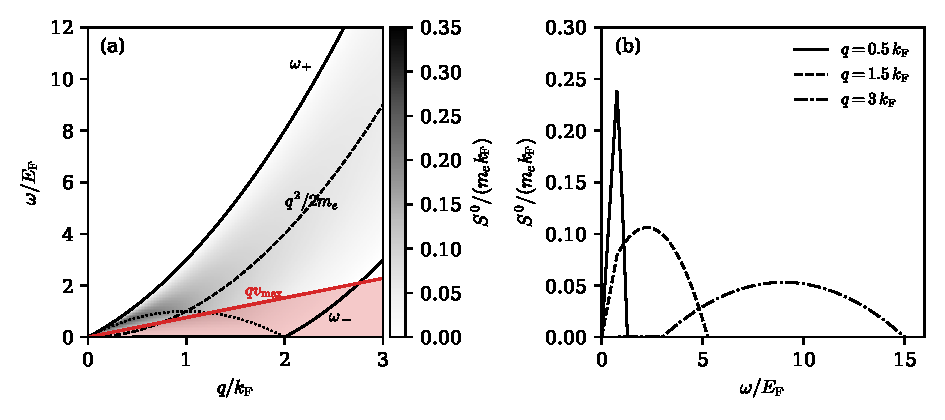
\includegraphics[width=\linewidth]{figures/ch04/fig4_2.pdf}
  \caption{Dynamic structure factor $S^0(q,\omega)$ of the non-interacting electron gas at zero temperature, in units of $m_ek_{\mathrm{F}}$, against the momentum transfer $q$ in units of the Fermi wavevector $k_{\mathrm{F}}$ and the energy $\omega$ in units of the Fermi energy $E_{\mathrm{F}} = k_{\mathrm{F}}^2/2m_e$. (a) Gray scale: $S^0$ inside the particle--hole continuum, bounded above by $\omega_+ = qv_{\mathrm{F}} + q^2/2m_e$ and below by $\omega_- = q^2/2m_e - qv_{\mathrm{F}}$ for $q > 2k_{\mathrm{F}}$ (solid). Below the dotted curve $\omega = qv_{\mathrm{F}} - q^2/2m_e$, $S^0 = m_e^2\omega/\pi q$ grows linearly in $\omega$; above it $S^0$ is a parabola in $\omega$ centered on the free recoil $q^2/2m_e$ (dashed). Red: the energies $\omega \le qv_{\mathrm{max}}$ that dark matter with the maximum halo speed $v_{\mathrm{max}} = 2.65\times10^{-3}$ can deposit, for the valence density of silicon, $\nd_e = \SI{2.00e23}{cm^{-3}}$ ($k_{\mathrm{F}} = \SI{3.57}{keV}$, $E_{\mathrm{F}} = \SI{12.5}{eV}$, $v_{\mathrm{max}} = 0.379\,v_{\mathrm{F}}$). (b) $S^0$ against $\omega$ at $q = 0.5$, 1.5 and $3\,k_{\mathrm{F}}$. At $q = 0.5\,k_{\mathrm{F}}$ the triangle peaks at $0.239\,m_ek_{\mathrm{F}}$ at $\omega = 0.75\,E_{\mathrm{F}}$; at $q = 3\,k_{\mathrm{F}}$ the parabola spans $\omega_- = 3\,E_{\mathrm{F}}$ to $\omega_+ = 15\,E_{\mathrm{F}}$. Every curve integrates to $2\pi\nd_e$ times the fraction of the Fermi sea that can take the momentum $q$, and its first moment is $\pi\nd_eq^2/m_e$.}
  \label{fig:4-gas}
\end{figure}

A gas of atoms is the other independent-particle target, and the one of \cref{sec:2.2}. There the rate off a bound electron was written with single-electron form factors, and the structure factor of a gas of atoms was identified by comparison with the rate formula of \cref{sec:1.5}. The many-body definition now produces it directly.

\begin{workedexample}{Hydrogen from the response matrix}\label{we:4-hydrogen}
Take $N_{\mathrm{at}}$ hydrogen atoms at fixed positions $\vect{R}_\ell$, far enough apart that their wavefunctions do not overlap, in a box of volume $\Vol$, with number density $\nd_T = N_{\mathrm{at}}/\Vol$. At any temperature far below the \SI{10.2}{eV} of the lowest excitation, every atom is in its 1s state. The density operator is a sum over atoms, $n_e(\vect{q}) = \sum_\ell\ee^{\ii\vect{q}\cdot\vect{r}_\ell}$, with $\vect{r}_\ell$ the position of the electron of atom $\ell$. Acting on the ground state it changes one atom at a time. A final state in which atom $\ell$ is in the level $f$ and all others are in 1s is reached by the term of atom $\ell$ alone, with the matrix element $\ee^{\ii\vect{q}\cdot\vect{R}_\ell}f_{1s\to f}(\vect{q})$, since $\vect{r}_\ell = \vect{R}_\ell + \vect{r}$ with $\vect{r}$ measured from the nucleus. The phase drops out of the square, every atom contributes the same, and \cref{eq:4.2-Sab} becomes
\begin{equation}
  S(\vect{q},\omega) = 2\pi\,\nd_T\sum_{f\ne 1s}|f_{1s\to f}(\vect{q})|^2\,\delta(\omega - E_f + E_{1s}) + \frac{2\pi}{\Vol}\,F_{1s}(q)^2\,\Bigl|\sum_\ell\ee^{\ii\vect{q}\cdot\vect{R}_\ell}\Bigr|^2\delta(\omega) ,
  \label{eq:4.2-hydrogen}
\end{equation}
with $F_{1s}$ the elastic form factor \cref{eq:2.2-F1s}. The inelastic term is the structure factor that \cref{sec:2.2} identified by comparing rates. Inserted into \cref{eq:2.5-golden}, it gives
\begin{equation*}
  \varGamma = \nd_T\int\frac{\dd^3q}{(2\pi)^3}\,|\tilde V(\vect{q})|^2\sum_f|f_{1s\to f}(\vect{q})|^2\,2\pi\,\delta(\omega_{\vect{q}} - E_f + E_{1s}) ,
\end{equation*}
which is $\nd_T$ times the $\sigma_Tv$ of one atom, \cref{eq:2.2-bound}. Each atom scatters on its own, and the rate counts atoms; the angle and halo averages of \cref{sec:2.2} then produce the spectrum \cref{eq:2.2-spectrum}. For an atom with several electrons, \cref{eq:4.2-S0} supplies what \cref{sec:2.2} added by hand: the initial orbitals must be occupied and the final ones empty.

The elastic term is where the atoms act together. At a fixed $\vect{q}$ its weight depends on the arrangement of the nuclei. For atoms at random positions the cross terms of $|\sum_\ell\ee^{\ii\vect{q}\cdot\vect{R}_\ell}|^2$ average to zero at $q \ne 0$ and the sum is $N_{\mathrm{at}}$. In a crystal the phases add at the reciprocal-lattice vectors instead. With fixed nuclei the elastic term deposits nothing; free atoms would take up the recoil of the whole atom.

The numbers of \cref{we:2-hydrogen} distribute the weight. At $q = q_0$ the integral of the inelastic term over $\omega$ is $2\pi\nd_T(1 - F_{1s}^2) = 2\pi\nd_T \times 0.59$, of which the $2p$ level takes $0.061$, about a tenth. The elastic term of the random gas carries $2\pi\nd_T \times 0.41$, and by \cref{eq:4.2-static} the two add to $S^{\mathrm{st}}(q_0) = 1$. A gas of independent atoms scatters incoherently at every $q$, and the form factor decides only how much of each scattering excites the atom.
\end{workedexample}

The free gas and the isolated atom are both exact for independent particles, and both miss what makes a solid's response many-body. The f-sum check above is one of a set of exact constraints on $S$ that hold whatever the interactions; \cref{sec:4.3} derives them from causality and commutators, and they are the tests that any computed structure factor of silicon has to pass.

\section{Causality and sum rules}\label{sec:4.3}

No calculation has the exact excited states of silicon, yet one number about its dynamic structure factor is known exactly at every momentum transfer: the energy-weighted integral $\int\dd\omega\,\omega\,S(\vect{q},\omega)$ equals $\pi\nd_eq^2/m_e$, fixed by the electron density alone. Another exact statement ties the real part of every response function to its imaginary part. The energy-weighted integral follows from a commutator, the link between real and imaginary parts from causality, and neither depends on the interactions, the temperature or the crystal structure. The treatment follows Refs.~\cite[Sects.~3.2--3.4]{giuliani2005quantum} and \cite[Chaps.~2 and 3]{pines1966theory}.

\subsection{Kramers--Kronig relations}

The spectral form \cref{eq:4.2-spectral} already reconstructs all of $R$ from $S$, and for a diagonal element it becomes a relation between the real and imaginary parts of $R$ itself. By the fluctuation--dissipation theorem \cref{eq:4.2-fdt}, the numerator $(1 - \ee^{-\beta\omega'})S_{aa}(\vect{q},\omega')$ is $-2\Imag R_{aa}(\vect{q},\omega')$, a real function of $\omega'$, and
\begin{equation*}
  R_{aa}(\vect{q},\omega) = -\frac{1}{\pi}\int_{-\infty}^{\infty}\dd\omega'\;\frac{\Imag R_{aa}(\vect{q},\omega')}{\omega - \omega' + \ii0^+} .
\end{equation*}
The Sokhotski--Plemelj formula \cref{eq:2.4-SP} splits the denominator into a principal value and $-\ii\pi\,\delta(\omega - \omega')$. The delta function returns $\Imag R_{aa}(\omega)$ on the right, as it must, and the principal value is the real part.
\begin{keyresult}[Kramers--Kronig relations]
For a response function analytic in the upper half plane and falling off at least as $1/|\omega|$,
\begin{equation}
  \begin{gathered}
  \Real R_{aa}(\vect{q},\omega) = \frac{1}{\pi}\operatorname{PV}\!\int_{-\infty}^{\infty}\dd\omega'\,\frac{\Imag R_{aa}(\vect{q},\omega')}{\omega' - \omega}, \\
  \Imag R_{aa}(\vect{q},\omega) = -\frac{1}{\pi}\operatorname{PV}\!\int_{-\infty}^{\infty}\dd\omega'\,\frac{\Real R_{aa}(\vect{q},\omega')}{\omega' - \omega} .
  \end{gathered}
  \label{eq:4.3-KK}
\end{equation}
The dissipative part of a response, at all frequencies, fixes its reactive part at each frequency, and conversely.
\end{keyresult}
These are \cref{eq:C.5-KK}~\cite{kronig1926theory,kramers1927diffusion}. The route through \cref{eq:4.2-spectral} yields the relation for the real part from the Lehmann form. The pair of relations needs less, just the two properties of \cref{sec:4.1}: $R$ is analytic in the upper half plane, and it falls off at large $|z|$, as $1/z^2$ for a density by \cref{eq:4.1-tail}. \Cref{app:C.5} derives them from these two properties alone, by closing the integral of $R(\omega')/(\omega' - z)$ over a large semicircle in the upper half plane (\cref{fig:4-kk}a). Since that argument refers to no eigenstates, the relations hold for a measured response, for a model such as the damped oscillator of \cref{we:4-oscillator}, and for any approximation that respects causality. \Cref{fig:4-kk}b rebuilds the real part of the oscillator response from its imaginary part alone. For an off-diagonal element the same argument applies to the analytic function $R_{ab}$, with the combination $\ii(R_{ab} - R_{ba}^*)$ of \cref{eq:4.2-fdt} in the role of the absorptive part.

\begin{figure}[tbp]
  \centering
  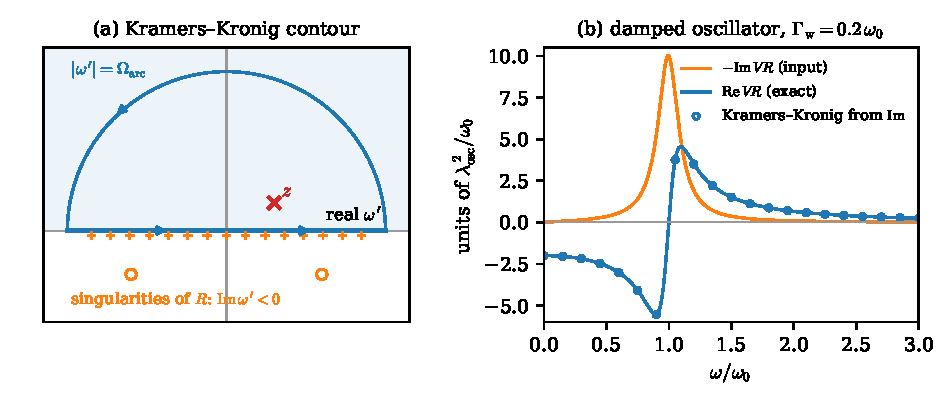
\includegraphics[width=\linewidth]{figures/ch04/fig4_3.pdf}
  \caption{The Kramers--Kronig relations. (a) The contour in the complex frequency plane $\omega'$: the real axis, closed by a semicircle of radius $\Omega_{\mathrm{arc}} \to \infty$ in the upper half plane (shaded), where the retarded response $R$ is analytic. The only singularity enclosed is the pole of $1/(\omega' - z)$ at a point $z$ of the upper half plane (cross). The singularities of $R$, the poles at transition energies that merge into a branch cut and the resonance poles of its continuation (schematic), all lie below the axis. Letting $z$ approach the real axis yields the relations. (b) Test on the damped oscillator with energy damping rate $\varGamma_{\mathrm{w}} = 0.2\,\omega_0$ and coupling $\lambda_{\mathrm{osc}}(d + d^\dagger)$. The real part of $\Vol R$ computed from $-\Imag\Vol R$ alone, with the folded relation for an even real part and an odd imaginary part (circles), agrees with the exact real part (line) to better than $10^{-11}\,\lambda_{\mathrm{osc}}^2/\omega_0$. At $\omega = 0$ both give $-2\lambda_{\mathrm{osc}}^2/\omega_0$.}
  \label{fig:4-kk}
\end{figure}

Most responses have a symmetry that folds the integral onto positive frequencies. For the density response of a target with inversion or time-reversal symmetry, the real part is even in $\omega$ and the imaginary part odd (\cref{sec:4.1}). Splitting the integral at zero and combining $1/(\omega' - \omega) + 1/(\omega' + \omega) = 2\omega'/(\omega'^2 - \omega^2)$,
\begin{equation}
  \Real R_{ee}(\vect{q},\omega) = \frac{2}{\pi}\operatorname{PV}\!\int_0^\infty\dd\omega'\,\frac{\omega'\,\Imag R_{ee}(\vect{q},\omega')}{\omega'^2 - \omega^2} ,
  \label{eq:4.3-KKhalf}
\end{equation}
which is \cref{eq:C.5-KKhalf}. Two limits of it carry physics. At $\omega = 0$, with $-2\Imag R_{ee} = (1 - \ee^{-\beta\omega})S$,
\begin{equation}
  R_{ee}(\vect{q},0) = -\frac{1}{\pi}\int_0^\infty\dd\omega\;\frac{(1 - \ee^{-\beta\omega})\,S(\vect{q},\omega)}{\omega} .
  \label{eq:4.3-static}
\end{equation}
The static response is an inverse moment of the structure factor, and it is negative because $S \ge 0$. At $T = 0$, inserting \cref{eq:4.2-Sab} returns the static limit of \cref{sec:4.1}, $\Vol R_{ee}(0) = -2\sum_f|\langle f|n_e(\vect{q})|0\rangle|^2/(E_f - E_0)$. Transitions at low energy dominate, since they are weighted by $1/\omega$: a target with a large gap is hard to deform. At large $\omega$, on the other hand, the denominator of \cref{eq:4.3-KKhalf} becomes $-\omega^2$, and $\Real R_{ee} \to -(2/\pi\omega^2)\int_0^\infty\dd\omega'\,\omega'\,\Imag R_{ee}$. The tail \cref{eq:4.1-tail} fixes the same coefficient by a double commutator. Equating the two, the energy-weighted integral of the absorptive part is fixed by an equal-time average. This is the first of the sum rules.

\subsection{Moments from commutators}

The $k$-th frequency moment of $S_{ab}$ weights each transition $i \to f$ with $\omega_{fi}^k$, where $\omega_{fi} = E_f - E_i$. The same power appears in a nested commutator. For any operator $X$, $\langle f|[H, X]|i\rangle = \omega_{fi}\langle f|X|i\rangle$, and $k$ commutators with $H$ give $\omega_{fi}^k$. Take operators with $O(-\vect{q}) = O(\vect{q})^\dagger$, as for every density, and write $[H, O_b]_k$ for $O_b$ commuted $k$ times with $H$. In the average of $[O_a^\dagger, [H, O_b]_k]$ over any state diagonal in the energy basis, with weights $p_i$, we insert a complete set $|f\rangle$ between the two operators. The term $O_a^\dagger[H, O_b]_k$ contributes $\sum_{i,f}p_i\,\omega_{fi}^k\langle i|O_a^\dagger|f\rangle\langle f|O_b|i\rangle$, the $k$-th moment of $\Vol S_{ab}(\vect{q},\omega)/2\pi$ by \cref{eq:4.2-Sab}. The term $[H, O_b]_kO_a^\dagger$ contributes $\sum_{i,f}p_i\,\omega_{if}^k\langle i|O_b|f\rangle\langle f|O_a^\dagger|i\rangle$. Since $O_b = O_b(-\vect{q})^\dagger$ and $O_a^\dagger = O_a(-\vect{q})$, this is $(-1)^k$ times the $k$-th moment of $\Vol S_{ba}(-\vect{q},\omega)/2\pi$. Altogether,
\begin{equation}
  \frac{1}{\Vol}\bigl\langle[O_a(\vect{q})^\dagger, [H, O_b(\vect{q})]_k]\bigr\rangle = \int_{-\infty}^{\infty}\frac{\dd\omega}{2\pi}\;\omega^k\,\bigl[S_{ab}(\vect{q},\omega) - (-1)^kS_{ba}(-\vect{q},\omega)\bigr] .
  \label{eq:4.3-moments}
\end{equation}
Since the derivation used only the stationarity of the state, \cref{eq:4.3-moments} holds in the Gibbs state at any temperature, in any eigenstate, and with any interactions. The integral runs over negative $\omega$ too, where a thermal target gives up energy. For $k = 0$ the left side is an equal-time commutator, and for densities, which commute with one another, it vanishes. The case $k = 1$ is the one with content.
\begin{keyresult}[First-moment identity]
For operators with $O(-\vect{q}) = O(\vect{q})^\dagger$ and any stationary state,
\begin{equation}
  \mathscr{M}^1_{ab}(\vect{q}) \equiv \frac{1}{\Vol}\bigl\langle[O_a(\vect{q})^\dagger, [H, O_b(\vect{q})]]\bigr\rangle = \int_{-\infty}^{\infty}\frac{\dd\omega}{2\pi}\;\omega\,\bigl[S_{ab}(\vect{q},\omega) + S_{ba}(-\vect{q},\omega)\bigr] .
  \label{eq:4.3-firstmoment}
\end{equation}
The energy-weighted spectrum, summed over $\pm\vect{q}$, is an equal-time double commutator.
\end{keyresult}
The first-moment matrix $\mathscr{M}^1_{ab}$ is the coefficient of $1/z^2$ in the tail \cref{eq:4.1-tail}, now read as a statement about $S$. On the diagonal, for a target with $S_{aa}(-\vect{q},\omega) = S_{aa}(\vect{q},\omega)$, it reads $\int\dd\omega\,\omega\,S_{aa} = \pi\mathscr{M}^1_{aa}$. A double commutator is often far simpler than the states it sums over, and this is why the identity is useful. The oscillator of \cref{we:4-oscillator} is the smallest example: $[O, [H, O]] = 2\lambda_{\mathrm{osc}}^2\omega_0$ is a number, and the first moment of its structure factor, $2\pi\lambda_{\mathrm{osc}}^2\omega_0$, does not depend on temperature, the result found from the populations in \cref{we:2-oscillator}. \Cref{chap:8} builds the higher moments into matrices for several operators.

\subsection{The f-sum rule}

For the electron density the double commutator is a number. The Hamiltonian of electrons and nuclei of \cref{sec:2.3} is the kinetic energy of the particles plus a potential energy that depends on their positions alone, and so do any external static potentials. The density $n_e(\vect{q}) = \sum_j\ee^{\ii\vect{q}\cdot\vect{r}_j}$ commutes with every position and with every nuclear momentum. Only the electron kinetic energy is left in $[H, n_e(\vect{q})]$. For one electron, $[\vect{p}, \ee^{\ii\vect{q}\cdot\vect{r}}] = \vect{q}\,\ee^{\ii\vect{q}\cdot\vect{r}}$, and $[\vect{p}^2, \ee^{\ii\vect{q}\cdot\vect{r}}] = \vect{p}\cdot\vect{q}\,\ee^{\ii\vect{q}\cdot\vect{r}} + \ee^{\ii\vect{q}\cdot\vect{r}}\,\vect{q}\cdot\vect{p}$. Summed over electrons,
\begin{equation}
  [H, n_e(\vect{q})] = \vect{q}\cdot\vect{j}_e(\vect{q}), \qquad \vect{j}_e(\vect{q}) = \sum_j\frac12\Bigl\{\frac{\vect{p}_j}{m_e},\,\ee^{\ii\vect{q}\cdot\vect{r}_j}\Bigr\} ,
  \label{eq:4.3-continuity}
\end{equation}
exactly, with $\{A, B\} = AB + BA$. This is the continuity equation in operator form. In the Heisenberg picture $\partial_tn_e(\vect{q},t) = \ii[H, n_e(\vect{q},t)] = \ii\vect{q}\cdot\vect{j}_e(\vect{q},t)$, the transform with $\ee^{+\ii\vect{q}\cdot\vect{r}}$ of $\partial_t\op{\nd}_e(\vect{r}) + \nabla\cdot\vect{j}_e(\vect{r}) = 0$ for the density operator of \cref{sec:4.2} and the current density in position space: density at $\vect{q}$ changes only because electrons carry it away. The symmetrized $\vect{j}_e(\vect{q})$ is what the literature calls the paramagnetic current, the current of the electrons when no vector potential acts.

The outer commutator, with $n_e(\vect{q})^\dagger$, is a number. Conjugating by the plane wave shifts the momentum, $\ee^{-\ii\vect{q}\cdot\vect{r}}\vect{p}\,\ee^{\ii\vect{q}\cdot\vect{r}} = \vect{p} + \vect{q}$, so $[\ee^{-\ii\vect{q}\cdot\vect{r}}, \vect{p}] = \vect{q}\,\ee^{-\ii\vect{q}\cdot\vect{r}}$, and each electron contributes $q^2/m_e$ to $[n_e(\vect{q})^\dagger, \vect{q}\cdot\vect{j}_e(\vect{q})]$ (\cref{app:D.6}). The commutator is $N_eq^2/m_e$ in every state, and $\mathscr{M}^1_{ee} = \nd_eq^2/m_e$.
\begin{keyresult}[f-sum rule]
For electrons that move in local potentials, at any temperature and with any interactions,
\begin{equation}
  \int_{-\infty}^{\infty}\dd\omega\;\omega\,S(\vect{q},\omega) = \frac{\pi\,\nd_e\,q^2}{m_e} \qquad \bigl(S(-\vect{q},\omega) = S(\vect{q},\omega)\bigr) ,
  \label{eq:4.3-fsum}
\end{equation}
and in general the same for the average of $S$ over $\vect{q}$ and $-\vect{q}$. The energy-weighted spectrum of density fluctuations counts the electrons.
\end{keyresult}
This is \cref{eq:A.7-fsum}~\cite[Sect.~3.4]{giuliani2005quantum}. The number $\nd_e$ counts every electron, core electrons included, and the nuclei may move. The normalization is $\pi$ over the whole real line. Many-body texts write the rule per particle and over positive frequencies, and the conversion is one line. At $T = 0$, $S$ vanishes for $\omega < 0$, and dividing by $2\pi\nd_e$ leads to $\int_0^\infty\dd\omega\,\omega\,S/(2\pi\nd_e) = q^2/2m_e$: per electron, and without the factor $2\pi$ of \cref{eq:4.2-Sab}, the first moment is the free recoil energy~\cite[Chap.~2]{pines1966theory}. At $T > 0$, detailed balance $S(\vect{q},-\omega) = \ee^{-\beta\omega}S(\vect{q},\omega)$ folds the negative frequencies onto the positive ones, $\int_0^\infty\dd\omega\,\omega\,(1 - \ee^{-\beta\omega})\,S = \pi\nd_eq^2/m_e$. By the fluctuation--dissipation theorem the integrand is $-2\omega\Imag R_{ee}$, which closes the loop with the large-$\omega$ limit of \cref{eq:4.3-KKhalf}.

The rule has a direct reading at large $q$. Divided by the total weight $2\pi\nd_eS^{\mathrm{st}}(\vect{q})$ of \cref{eq:4.2-static}, it gives the mean energy deposited at $T = 0$, $q^2/[2m_eS^{\mathrm{st}}(\vect{q})]$. Where $S^{\mathrm{st}} \to 1$ and the dark matter scatters on one electron at a time, the mean energy deposited tends to the free recoil energy, however strongly the electron is bound. Binding moves the weight around, broadening it as in the impulse approximation of \cref{we:4-gas}, but it cannot shift its center. At small $q$, where $S^{\mathrm{st}}$ is suppressed, the mean energy lies far above $q^2/2m_e$, and in the interacting electron gas the plasmon carries all of the sum (\cref{sec:4.5}).

The right side of \cref{eq:4.3-fsum} defines the frequency scale of the electrons. With $e^2 = 4\pi\alpha$,
\begin{equation}
  \frac{\pi\nd_eq^2}{m_e} = \frac{\pi q^2}{e^2}\,\omega_p^2, \qquad \omega_p^2 = \frac{e^2\nd_e}{m_e} ,
  \label{eq:4.3-wp}
\end{equation}
where $\omega_p$ is the plasma frequency, the frequency at which the electrons, treated as free, would oscillate together against a uniform positive background (\cref{sec:4.5}). For the valence density of silicon, $\nd_e = \SI{2.00e23}{cm^{-3}}$, $\omega_p = \SI{16.6}{eV}$; for all 14 electrons per atom, $\SI{7.00e23}{cm^{-3}}$, it is \SI{31.1}{eV}. \Cref{sec:4.4} converts \cref{eq:4.3-fsum} into the form $\int_0^\infty\dd\omega\,\omega\,L = (\pi/2)\,\omega_p^2$ for the loss function, the form that a computed or measured spectrum is usually tested against.

\subsection{Nonlocal potentials and the f-sum rule}

The derivation of \cref{eq:4.3-fsum} needed one hypothesis: every potential energy in $H$ is a function of positions. The Hamiltonian of electrons and nuclei satisfies it, but the effective Hamiltonians with which solids are computed often do not. A pseudopotential (\cref{sec:3.5}) replaces the nucleus and the core electrons by a local potential and a nonlocal part $V_{\mathrm{NL}}$, the sum of projections \cref{eq:E.2-KB}, which acts on a valence wavefunction through its values over a whole core region rather than at one point. The Fock exchange operator is nonlocal in the same sense. Such an operator does not commute with $\ee^{\ii\vect{q}\cdot\vect{r}}$, the commutator $[H, n_e(\vect{q})]$ acquires $[V_{\mathrm{NL}}, n_e(\vect{q})]$ besides $\vect{q}\cdot\vect{j}_e$, and
\begin{equation}
  \mathscr{M}^1_{ee}(\vect{q}) = \frac{\nd_eq^2}{m_e} + \frac{1}{\Vol}\bigl\langle[n_e(\vect{q})^\dagger, [V_{\mathrm{NL}}, n_e(\vect{q})]]\bigr\rangle ,
  \label{eq:4.3-fsumNL}
\end{equation}
with $\nd_e$ now the density of the valence electrons that the calculation keeps. The exact rule is not violated, since it belongs to the full Hamiltonian. The pseudo-Hamiltonian is a device that reproduces the valence states outside the cores, not their every commutator. A pseudo-wavefunction is smooth where the true valence state oscillates to stay orthogonal to the core states, and part of what that oscillation does is carried by $V_{\mathrm{NL}}$. The extra term is a sum of projections and costs almost nothing to evaluate. \Cref{app:E.2} writes it for one electron, \cref{eq:E.2-fsumNL}, and finds that in a representative silicon calculation this term and the truncated band sum together put the computed sum 12 to 19 percent below the local value at small $q$. A sum-rule test of a pseudopotential calculation therefore compares with \cref{eq:4.3-fsumNL}, not with \cref{eq:4.3-fsum}. At $q \to 0$ the same algebra turns the momentum into the velocity $\ii[H, \vect{r}] = \vect{p}/m_e + \ii[V_{\mathrm{NL}}, \vect{r}]$, the form that Ismail-Beigi, Chang and Louie derived for the coupling of a nonlocal potential to a long-wavelength field~\cite{ismailbeigi2001coupling}.

Relativistic electrons break the hypothesis in a different way. To order $1/m_e^2$, an electron in a one-body potential $U_1(\vect{r})$ has three corrections, derived in \cref{app:C.15}: the mass--velocity term $-\vect{p}^4/8m_e^3$, the Darwin term $\nabla^2U_1/8m_e^2$ and the spin--orbit term $\vect{\sigma}\cdot(\nabla U_1\times\vect{p})/4m_e^2$. The Darwin and spin--orbit terms drop out of the double commutator, and the mass--velocity term does not (\cref{app:D.6}). In an atom, or in a crystal of cubic symmetry,
\begin{equation}
  \mathscr{M}^1_{ee}(\vect{q}) = \frac{\nd_eq^2}{m_e}\Bigl[1 - \frac53\,\frac{\bar K}{m_e} - \frac{q^2}{4m_e^2}\Bigr] ,
  \label{eq:4.3-mv}
\end{equation}
where $\bar K$ is the mean kinetic energy per electron. A moving electron is heavier, and the f-sum, which counts electrons weighted by $1/m_e$, is reduced by the relative order $\bar K/m_e$. For silicon the virial theorem makes the total kinetic energy of the atom minus its total energy, \SI{7.86}{keV} from the Hartree--Fock value of $-288.854$ hartree~\cite{bunge1993roothaan}, so $\bar K = \SI{561}{eV}$ and $(5/3)\bar K/m_e = 1.8\times10^{-3}$, or 0.026 electrons per atom. The two 1s electrons dominate: each has a kinetic energy near $Z^2\alpha^2m_e/2 = \SI{2.67}{keV}$, which reduces its own share of the sum by $8.7\times10^{-3}$. The term in $q^2$ is $2.7\times10^{-3}$ at the \SI{53}{keV} that a \SI{10}{MeV} particle can transfer at most. The two-body Breit terms, which depend on the momenta of pairs of electrons, contribute at the same relative order, and we do not estimate them. All of these corrections lie below the accuracy of any calculation of $S$ for dark matter. They do mean, however, that an all-electron relativistic calculation with positive-energy states alone should not reproduce \cref{eq:4.3-fsum} to better than a few parts in $10^3$. The expansion in $1/m_e$ is this positive-energy statement. The full Dirac Hamiltonian is linear in the momentum, its double commutator with the density vanishes, and the f-sum is then carried by the creation of electron--positron pairs, at energies near $2m_e$.

The nuclei obey the same algebra as the electrons. With the density $n_\kappa(\vect{q}) = \sum_{I\in\kappa}\ee^{\ii\vect{q}\cdot\vect{X}_I}$ of the nuclei of species $\kappa$, their mass $M_\kappa$ and number density $\nd_\kappa$ (\cref{sec:2.3}), the kinetic energy of the nuclei gives $[H, n_\kappa(\vect{q})] = \vect{q}\cdot\vect{j}_\kappa(\vect{q})$, with a current $\vect{j}_\kappa$ built like $\vect{j}_e$ from nuclear momenta and $M_\kappa$. A current of one species contains only that species' momenta, and it commutes with the density of every other species. The mixed double commutators therefore vanish.
\begin{keyresult}[Species-resolved f-sum rule]
For electrons and nuclei in local potentials, with $s, s' \in \{e, \kappa\}$ and $m_s$ equal to $m_e$ or $M_\kappa$,
\begin{equation}
  \mathscr{M}^1_{ss'}(\vect{q}) = \delta_{ss'}\,\frac{q^2\,\nd_s}{m_s} .
  \label{eq:4.3-species}
\end{equation}
Each species has its own f-sum, fixed by its density and mass, and the energy-weighted electron--nucleus interference vanishes.
\end{keyresult}
The nuclear rule, $\int\dd\omega\,\omega\,S_{\kappa\kappa} = \pi\nd_\kappa q^2/M_\kappa$, makes the mean energy deposited on a nucleus equal to its free recoil energy $q^2/2M_\kappa$ wherever $S^{\mathrm{st}}$ of the nuclei is one, the incoherent limit of the lattice response of \cref{chap:5,chap:6}. The mixed rule has a less obvious consequence. For a target with inversion symmetry, $S_{\kappa e}(-\vect{q},\omega) = S_{\kappa e}(\vect{q},\omega)$, which Hermiticity makes $S_{e\kappa}(\vect{q},\omega)^*$, and \cref{eq:4.3-firstmoment} with \cref{eq:4.3-species} reads $\int\dd\omega\,\omega\Real S_{e\kappa}(\vect{q},\omega) = 0$. At $T = 0$ the integral runs over $\omega > 0$ alone, and the real part of the electron--nucleus interference must change sign: the electrons follow a recoiling nucleus in phase at some energies and against it at others. A computed interference spectrum of one sign, for the Migdal effect for instance (\cref{chap:8}), is wrong. Finally, for the total charge density $n_Z = -n_e + \sum_\kappa Z_\kappa n_\kappa$ of \cref{sec:2.3}, the diagonal terms add: $\mathscr{M}^1_{ZZ} = q^2[\nd_e/m_e + \sum_\kappa Z_\kappa^2\nd_\kappa/M_\kappa]$. For silicon, with $Z_\kappa = 14$ and all 14 electrons per atom, the nuclear share is $14\,m_e/M_\kappa = 2.73\times10^{-4}$. A probe of the total charge, such as a dark photon, sees an f-sum set by the electrons to that accuracy.

\subsection{Oscillator strengths}

For a single atom the f-sum rule becomes a statement about its spectral lines. Take an atom with $Z$ electrons in its ground state $|0\rangle$. Its double commutator is $Zq^2/m_e$, and inserting the excited states $|n\rangle$ as in \cref{eq:4.3-moments} turns it into $\sum_n(E_n - E_0)\bigl[|\langle n|n_e(\vect{q})|0\rangle|^2 + |\langle n|n_e(-\vect{q})|0\rangle|^2\bigr]$. For a ground state with inversion symmetry the two terms are equal, and
\begin{equation}
  \sum_n(E_n - E_0)\,\bigl|\langle n|n_e(\vect{q})|0\rangle\bigr|^2 = \frac{Zq^2}{2m_e} ,
  \label{eq:4.3-atomq}
\end{equation}
at every $\vect{q}$. For the gas of atoms of \cref{we:4-hydrogen}, whose structure factor is $2\pi\nd_T$ times the sum of these transition weights, it is \cref{eq:4.3-fsum} with $\nd_e = Z\nd_T$. As $q \to 0$, the matrix element to an excited state starts at first order in $q$, $\langle n|n_e(\vect{q})|0\rangle = \ii\vect{q}\cdot\langle n|\sum_j\vect{r}_j|0\rangle$, since the zeroth order vanishes by orthogonality. The dipole matrix elements that remain define the oscillator strengths,
\begin{equation}
  f^{\mathrm{osc}}_{n0} = 2m_e\,(E_n - E_0)\,\Bigl|\langle n|\sum_j\hat{\vect{q}}\cdot\vect{r}_j|0\rangle\Bigr|^2 ,
  \label{eq:4.3-osc}
\end{equation}
and \cref{eq:4.3-atomq} divided by $q^2/2m_e$ becomes the Thomas--Reiche--Kuhn rule~\cite{thomas1925zahl,reiche1925zahl,kuhn1925gesamtstarke},
\begin{equation}
  \sum_nf^{\mathrm{osc}}_{n0} = Z ,
  \label{eq:4.3-TRK}
\end{equation}
where the sum includes the continuum, as an integral of the oscillator-strength density $\dd f^{\mathrm{osc}}/\dd\omega$ over the energy $\omega = E_n - E_0$ of the absorbed quantum. In the classical picture an atom was a set of electrons bound by springs, and $f^{\mathrm{osc}}_{n0}$ counted how many of them oscillated at the frequency of line $n$. The rule says that the lines of an atom share exactly $Z$ such classical electrons. Its use is as a check. A table of computed or measured oscillator strengths, or of photoabsorption cross-sections, must add up to $Z$, and a set of ionization form factors (\cref{eq:2.2-fion}) must satisfy \cref{eq:4.3-atomq} at each $q$, which tests the normalization of the continuum.

\begin{workedexample}{The Thomas--Reiche--Kuhn sum of hydrogen}\label{we:4-trk}
For hydrogen, $Z = 1$, and the oscillator strengths from 1s are known in closed form~\cite[Sect.~61]{bethe1957quantum}. The dipole operator reaches only p states. For the bound levels,
\begin{equation*}
  f^{\mathrm{osc}}_{np,1s} = \frac{2^8\,n^5\,(n - 1)^{2n-4}}{3\,(n + 1)^{2n+4}} ,
\end{equation*}
which is 0.4162 for 2p, and 0.0791, 0.0290 and 0.0139 for 3p to 5p. For large $n$, $[(n - 1)/(n + 1)]^{2n} \to \ee^{-4}$ and $f^{\mathrm{osc}}_{np,1s} \to (2^8/3)\,\ee^{-4}/n^3$. The levels crowd toward the binding energy $E_B = \alpha^2m_e/2 = \SI{13.6}{eV}$ of \cref{sec:2.2} with spacing $2E_B/n^3$, and their strength per unit energy tends to $(2^7/3)\,\ee^{-4}/E_B = 0.782/E_B$. The continuum takes over at the same value. With the Coulomb parameter of \cref{sec:2.2} for the ejected electron, $\xi_{\mathrm{C}} = \alpha m_e/p = [E_B/(\omega - E_B)]^{1/2}$ for $\omega > E_B$, its density is~\cite[Sect.~61]{bethe1957quantum}
\begin{equation*}
  \frac{\dd f^{\mathrm{osc}}}{\dd\omega} = \frac{2^7}{3E_B}\Bigl(\frac{E_B}{\omega}\Bigr)^4\,\frac{\exp(-4\xi_{\mathrm{C}}\operatorname{arccot}\xi_{\mathrm{C}})}{1 - \ee^{-2\pi\xi_{\mathrm{C}}}} ,
\end{equation*}
which tends to $0.782/E_B$ at threshold, where $\xi_{\mathrm{C}} \to \infty$ and $\xi_{\mathrm{C}}\operatorname{arccot}\xi_{\mathrm{C}} \to 1$.

Adding up (\cref{fig:4-trk}a), the bound levels carry 0.565, of which 2p alone carries 0.416 and the first three 0.524. The continuum carries 0.435: 0.316 within $E_B$ of the threshold, and only 0.0042 above $10E_B$, since at large $\omega$, where $\xi_{\mathrm{C}} \to 0$, the density falls as $\omega^{-7/2}$. The total is $1.000$, as \cref{eq:4.3-TRK} requires. A calculation that keeps the bound states alone fails the check by 43 percent: the continuum, which is the ionization channel of \cref{sec:2.2}, is not a correction.

The finite-$q$ rule \cref{eq:4.3-atomq} tests the same states at a dark-matter momentum transfer. At $q_0 = \alpha m_e$ its right side is exactly $q_0^2/2m_e = \alpha^2m_e/2 = E_B$. The 2p level has $|f_{1s\to2p}(q_0)|^2 = 0.061$ (\cref{we:2-hydrogen}) at the energy $\tfrac34E_B$, and contributes $0.046\,E_B$, under 5 percent of the sum, although it takes a tenth of the inelastic weight at that $q$ (\cref{we:4-hydrogen}). The rest of the energy-weighted sum lies in the continuum, at energies $\sim E_B$ and above.
\end{workedexample}

\begin{workedexample}{The f-sum of the free electron gas}\label{we:4-gasfsum}
\Cref{we:4-gas} obtained the first moment of $S^0$ from the sum over occupied states. The closed form \cref{eq:4.2-gas} must reproduce it, and integrating it shows where the weight sits. For $q > 2k_{\mathrm{F}}$, $S^0$ is the parabola between $\omega_-$ and $\omega_+$. We change variable to $x = m_e\omega/q - q/2$, which runs from $-k_{\mathrm{F}}$ to $k_{\mathrm{F}}$. Then $\omega = (q/m_e)(x + q/2)$, $\dd\omega = (q/m_e)\,\dd x$ and $S^0 = (m_e/2\pi q)(k_{\mathrm{F}}^2 - x^2)$, so that
\begin{equation*}
  \int\dd\omega\;\omega\,S^0 = \frac{q}{2\pi m_e}\int_{-k_{\mathrm{F}}}^{k_{\mathrm{F}}}\dd x\,\Bigl(x + \frac q2\Bigr)(k_{\mathrm{F}}^2 - x^2) = \frac{q}{2\pi m_e}\,\frac q2\,\frac{4k_{\mathrm{F}}^3}{3} = \frac{q^2k_{\mathrm{F}}^3}{3\pi m_e} .
\end{equation*}
The term odd in $x$, the Doppler shift from the motion of the struck electron, integrates to zero, and with $\nd_e = k_{\mathrm{F}}^3/3\pi^2$ the result is $\pi\nd_eq^2/m_e$. For $q < 2k_{\mathrm{F}}$ the linear region, $0 < \omega < \omega_1 = (q/m_e)(k_{\mathrm{F}} - q/2)$, contributes $\int\dd\omega\,\omega\,m_e^2\omega/\pi q = m_e^2\omega_1^3/3\pi q = q^2(k_{\mathrm{F}} - q/2)^3/3\pi m_e$. That is the fraction $(1 - q/2k_{\mathrm{F}})^3$ of the sum, $27/64 = 0.42$ at $q = k_{\mathrm{F}}/2$, and the parabola carries the rest. As $q \to 0$ the linear region carries the whole sum, and the mean energy $(q^2/2m_e)/S^{\mathrm{st}}$, with $S^{\mathrm{st}} \to 3q/4k_{\mathrm{F}}$, is $\tfrac23qv_{\mathrm{F}}$, which vanishes. A gapless target can place its f-sum at vanishing energies, but only because its long-wavelength fluctuations are suppressed by the Pauli hole of \cref{sec:4.2}.

A gap changes the balance. Take the valence electrons of an insulator at $T = 0$, with the nuclei clamped and the potentials local, and their share of the f-sum, collected below the core edges (\cref{we:4-sifsum}). Their inelastic $S$ vanishes below the gap $\Eg$, so $\Eg\int\dd\omega\,S \le \int\dd\omega\,\omega\,S$. By \cref{eq:4.2-static,eq:4.3-fsum}, the inelastic part of the static structure factor then obeys, to the accuracy with which the valence electrons carry their own f-sum (about 2 percent in silicon, \cref{we:4-sifsum}),
\begin{equation*}
  S^{\mathrm{st}}(\vect{q}) \le \frac{q^2}{2m_e\Eg} .
\end{equation*}
At the valence density of silicon, $k_{\mathrm{F}} = \SI{3.57}{keV}$, and with $\Eg = \SI{1.17}{eV}$ this bound lies below the free-gas value $3q/4k_{\mathrm{F}}$ for $q < 3m_e\Eg/2k_{\mathrm{F}} = \SI{0.25}{keV}$; at $q = \SI{0.1}{keV}$ it is 0.40 of it. The long-wavelength density fluctuations of an insulator vanish as $q^2$, not as $q$, and the f-sum rule is what turns the gap into this statement.
\end{workedexample}

\begin{workedexample}{The f-sum of silicon}\label{we:4-sifsum}
A silicon atom has 14 electrons, four in the valence shell and ten in the core, two 1s and eight 2s and 2p. With the full, local Hamiltonian the f-sum counts all of them, and at $q \to 0$ the Thomas--Reiche--Kuhn rule \cref{eq:4.3-TRK}, applied per atom of the crystal, gives 14. The four valence electrons absorb from the gap upward; the core electrons cannot absorb below their binding energies, which put the L edge near \SI{100}{eV} and the K edge at \SI{1.84}{keV}.

Henke, Gullikson and Davis tabulated the photoabsorption of silicon from \SI{50}{eV} to \SI{30}{keV}. Their current distribution extends down to \SI{30}{eV}, and we integrate it from there. They express it through the imaginary part $f_2(\omega)$ of the atomic scattering factor, which in the convention of the tables is $f_2 = (\pi/2)\,\omega\,\dd f^{\mathrm{osc}}/\dd\omega$ per atom~\cite{henke1993xray}. The two edges appear in the tables as steps of $f_2$, at \SI{99.8}{eV} and \SI{1.839}{keV}. Integrating $2f_2/\pi\omega$ over the regions they bound gives 0.35 between \SI{30}{eV} and the L edge, 8.46 between the L and K edges, and 1.61 above the K edge. Of the last, 0.007 comes from extending the last decade of the tables beyond \SI{30}{keV} as a power law. Above \SI{30}{eV} the tables therefore hold 10.42 of the 14. The rule then requires 3.58 below \SI{30}{eV} (3.55 with the mass--velocity reduction of \cref{eq:4.3-mv}), and 3.93 below the L edge, against the four valence electrons (\cref{fig:4-trk}b).

The saturation is slow and has the same pattern in each region. The valence part is complete to 2 percent below the L edge, at six times $\omega_p$. The region between the edges collects 97 percent of its strength by \SI{1}{keV}, ten times its edge energy, and the region above the K edge collects 84 percent by \SI{5}{keV} and 96 percent by \SI{10}{keV}. Each shell gathers its strength over energies from its edge to several times it, with the slow $\omega^{-5/2}$ approach of the remaining strength that hydrogen showed.

The regions are not the shells. The region above the K edge holds 1.61, not 2. The 1s electrons cannot be promoted into the full 2p shell, a transition that carries 0.42 of the sum in hydrogen. In a picture of independent electrons, the rule holds for each electron only when transitions into occupied orbitals are counted too, upward with positive and downward with negative strength. In the atom both members of such a pair are blocked by the Pauli principle, and since their strengths cancel, the total stays 14 while strength moves from the inner shells to the outer ones. The excess of the region between the edges over 8 is the receiving side of this transfer, together with the overlap of tails: the L absorption continues above the K edge, and the valence absorption continues above the L edge.

For dark matter the split matters at finite $q$. At $q \to 0$ the core part of the sum lies above \SI{100}{eV}, far from the valence part. At larger $q$ the valence weight moves toward the free recoil energy $q^2/2m_e$, which is \SI{98}{eV} at $q = \SI{10}{keV}$, where the dark matter can deposit at most $qv_{\mathrm{max}} = \SI{26.5}{eV}$. A valence-only calculation tested against its f-sum at such momentum transfers must follow the valence spectrum to energies where the core shells it omits absorb as well. The sum rule constrains the total over all energies, not the low-energy corner that the dark matter samples.
\end{workedexample}

\begin{figure}[tbp]
  \centering
  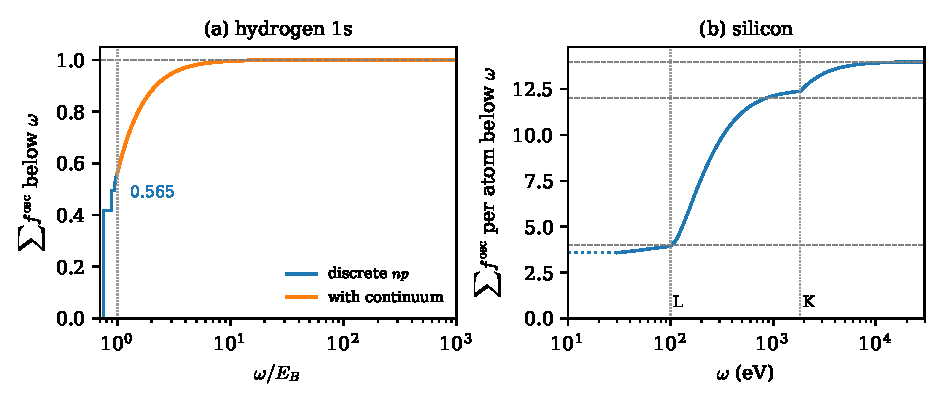
\includegraphics[width=\linewidth]{figures/ch04/fig4_3b.pdf}
  \caption{The Thomas--Reiche--Kuhn sum accumulated with energy. (a) Hydrogen in its ground state: oscillator strength of all transitions below the absorbed energy $\omega$, in units of the binding energy $E_B = \SI{13.6}{eV}$, from the closed forms of Bethe and Salpeter. The bound 1s--$np$ lines (steps, starting with 2p at $\tfrac34E_B$) carry 0.565 and the continuum 0.435; the total is one electron (dashed). (b) Silicon, per atom: oscillator strength below $\omega$ from the photoabsorption tables of Henke and coworkers above \SI{30}{eV}, integrated as $\dd f^{\mathrm{osc}}/\dd\omega = 2f_2/\pi\omega$, and offset so that the total, with the region above \SI{30}{keV} extrapolated as a power law, is 14. The offset, 3.58, is the strength below \SI{30}{eV} that the rule requires (dotted). Dashed lines mark 4 valence electrons, 4 + 8 and 14; dotted vertical lines the L and K edges at \SI{99.8}{eV} and \SI{1.839}{keV}.}
  \label{fig:4-trk}
\end{figure}

\section{Screening and the dielectric function}\label{sec:4.4}

A dark-matter particle that transfers the typical momentum $q_0 = \alpha m_e = \SI{3.73}{keV}$ to silicon does not meet the bare valence electrons. Its potential pushes the electrons it reaches, the displaced charge produces a potential of its own, and the electrons respond to the sum. A crude estimate (\cref{we:4-tf}) reduces the potential at $q_0$ by a factor of about two, and the rate, which goes as its square, by about five. Full calculations for silicon and germanium find that screening changes the rate by a factor of a few~\cite{knapen2021dark}. The response function $R_{ee}$ of \cref{sec:4.1} contains all of this, but it mixes two kinds of physics: the long-range Coulomb field of the displaced charge, which is classical and universal, and everything else, which depends on the material. Separating the two defines the dielectric function. We will see that the structure factor that sets the rate is, up to a factor $q^2$, the imaginary part of the inverse dielectric function, the loss function, which is measured in optical and electron-energy-loss experiments. The treatment follows Refs.~\cite[Chaps.~3 and 5]{giuliani2005quantum} and \cite{onida2002electronic}.

\subsection{Proper response and the dielectric function}

Apply to the electrons an external potential energy that varies as $\ee^{\ii\vect{q}\cdot\vect{r}}$, with amplitude $\phi_{\mathrm{ext}}(\vect{q},\omega)$ at frequency $\omega$, and keep the nuclei clamped. By the Kubo formula \cref{eq:4.1-kubo}, the electron density develops a ripple with amplitude $\delta\nd_e = R_{ee}(\vect{q},\omega)\,\phi_{\mathrm{ext}}$, where $\delta\nd_e$ is $\delta\langle n_e(\vect{q})^\dagger\rangle/\Vol$, the coefficient of $\ee^{\ii\vect{q}\cdot\vect{r}}$ in the induced density (\cref{sec:4.1}). The ripple is a charge, and by Coulomb's law it acts on every electron with the potential energy $v_{\mathrm{C}}(q)\,\delta\nd_e$, with the kernel \cref{eq:2.3-vC}. Each electron then feels the total potential energy
\begin{equation}
  \phi_{\mathrm{tot}}(\vect{q},\omega) = \phi_{\mathrm{ext}}(\vect{q},\omega) + v_{\mathrm{C}}(q)\,\delta\nd_e(\vect{q},\omega) ,
  \label{eq:4.4-phitot}
\end{equation}
the external part plus the Hartree potential of the induced density. The induced density is a response to $\phi_{\mathrm{tot}}$ as much as to $\phi_{\mathrm{ext}}$, and the response to the total potential is the one that excludes the long-range field. We define it as the Coulomb-proper (or irreducible) response $\tilde R_{ee}$,
\begin{equation}
  \delta\nd_e = \tilde R_{ee}(\vect{q},\omega)\,\phi_{\mathrm{tot}}(\vect{q},\omega) .
  \label{eq:4.4-proper}
\end{equation}
It contains every effect of the interactions except the classical Hartree field at the wavevector $\vect{q}$: exchange, correlation, the band structure, the excitations of the target. In contrast, $R_{ee}$ is the improper response.

Inserting \cref{eq:4.4-phitot} into \cref{eq:4.4-proper} and comparing with $\delta\nd_e = R_{ee}\phi_{\mathrm{ext}}$, for any $\phi_{\mathrm{ext}}$,
\begin{equation}
  R_{ee} = \tilde R_{ee} + \tilde R_{ee}\,v_{\mathrm{C}}\,R_{ee}, \qquad R_{ee} = \frac{\tilde R_{ee}}{1 - v_{\mathrm{C}}\tilde R_{ee}} .
  \label{eq:4.4-dyson}
\end{equation}
This is a Dyson equation of the form \cref{eq:C.7-dyson}, with $\tilde R_{ee}$ as the bare object and $v_{\mathrm{C}}$ as the kernel. Iterating it gives the geometric series
\begin{equation*}
  R_{ee} = \tilde R_{ee} + \tilde R_{ee}v_{\mathrm{C}}\tilde R_{ee} + \tilde R_{ee}v_{\mathrm{C}}\tilde R_{ee}v_{\mathrm{C}}\tilde R_{ee} + \cdots ,
\end{equation*}
which has a direct reading. The external potential polarizes the electrons, the polarization creates a Coulomb potential, that potential polarizes them again, and so on. \Cref{fig:4-series} draws the series with the proper parts as blobs joined by Coulomb lines. The name ``proper'' says that $\tilde R_{ee}$ is the part of the response that cannot be cut into two pieces joined by a single Coulomb line at the momentum $\vect{q}$; \cref{sec:4.8} reads the figure as a sum of Feynman diagrams. The closed form holds beyond the radius of convergence of the series, and its poles, at $1 - v_{\mathrm{C}}\tilde R_{ee} = 0$, are oscillations that the electrons sustain without an external field.

\begin{figure}[tbp]
  \centering
  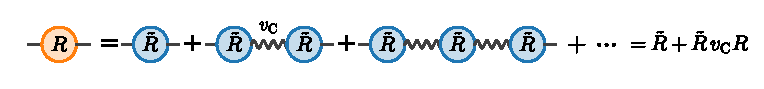
\includegraphics[width=\linewidth]{figures/ch04/fig4_4.pdf}
  \caption{Schematic of the relation between the density response $R$ and its Coulomb-proper part $\tilde R$. Each shaded blob is the proper response of the electrons, which includes every interaction effect except the long-range Coulomb field at the momentum transfer $\vect{q}$. Each wavy line is the Coulomb kernel $v_{\mathrm{C}}(q) = e^2/q^2$, which carries the potential of the charge induced in one blob to the next. Summed, the chain is the geometric series $R = \tilde R + \tilde Rv_{\mathrm{C}}\tilde R + \cdots$, whose closed form is $R = \tilde R + \tilde Rv_{\mathrm{C}}R$. The drawing is a schematic, not a set of Feynman rules.}
  \label{fig:4-series}
\end{figure}

The ratio of the external to the total potential is the dielectric function. From \cref{eq:4.4-phitot,eq:4.4-proper}, $\phi_{\mathrm{ext}} = (1 - v_{\mathrm{C}}\tilde R_{ee})\,\phi_{\mathrm{tot}}$ and $\phi_{\mathrm{tot}} = (1 + v_{\mathrm{C}}R_{ee})\,\phi_{\mathrm{ext}}$. Hence
\begin{equation}
  \varepsilon(\vect{q},\omega) \equiv \frac{\phi_{\mathrm{ext}}}{\phi_{\mathrm{tot}}} = 1 - v_{\mathrm{C}}(q)\,\tilde R_{ee}(\vect{q},\omega), \qquad
  \varepsilon^{-1}(\vect{q},\omega) = 1 + v_{\mathrm{C}}(q)\,R_{ee}(\vect{q},\omega) ,
  \label{eq:4.4-eps}
\end{equation}
and the two forms are each other's inverse by \cref{eq:4.4-dyson}. These are the relations \cref{eq:A.7-eps,eq:A.7-L} stated in \cref{app:A.7}, and the second is Ref.~\cite[Eq.~(5)]{knapen2021dark} in our units. We write $\varepsilon = \varepsilon_1 + \ii\varepsilon_2$. The classical reading is the familiar one. In Heaviside--Lorentz units the external charge is the source of $\vect{D}$ and the total charge the source of $\vect{E}$. For a longitudinal field the potential energies are proportional to the potentials, so $\varepsilon$ is the ratio $D/E$ of the Fourier components, the dielectric function of classical electromagnetism, now for every $\vect{q}$ and $\omega$. It is the longitudinal dielectric function, because a potential produces a field along $\vect{q}$.

The inverse function $\varepsilon^{-1} - 1 = v_{\mathrm{C}}R_{ee}$ is a retarded response, the induced potential per unit external one, and it has every property \cref{sec:4.1,sec:4.3} proved for $R_{ee}$: analyticity in the upper half plane, the Kramers--Kronig relations, and $\Imag\varepsilon^{-1} \le 0$ for $\omega > 0$. The function $\varepsilon - 1$ obeys the Kramers--Kronig relations only because a stable target has no zeros of $\varepsilon$ in the upper half plane (\cref{eq:C.5-KKeps}). The static limit of $\varepsilon^{-1}v_{\mathrm{C}}$ is the statically screened Coulomb interaction: an external point charge, or a second electron held at rest, acts through $v_{\mathrm{C}}(q)/\varepsilon(\vect{q},0)$ rather than $v_{\mathrm{C}}(q)$ (\cref{sec:4.8} uses it in the electron self-energy). At small $q$, $v_{\mathrm{C}}$ grows as $1/q^2$, and this is where screening matters most.

In an insulator the static dielectric function at long wavelength is finite. With the lattice clamped, its value $\varepsilon_\infty = \varepsilon(\vect{q}\to0, \omega\to0)$ is the electronic, or high-frequency, dielectric constant, so called because it is measured at frequencies above those of the lattice vibrations and below the gap; the static constant $\varepsilon_0$ with the lattice included is the subject of \cref{sec:5.5}. For silicon $\varepsilon_\infty = 11.7$~\cite{franta2017temperature}: a static charge in the crystal is screened to a twelfth of its bare strength at distances of many cells. Where $\varepsilon_1$ crosses zero and $\varepsilon_2$ is small, the external potential produces a large total one, and the electrons oscillate collectively. This is the plasmon, a pole of \cref{eq:4.4-dyson} near the real axis, which appears as a peak of $\Imag(-\varepsilon^{-1})$; \cref{sec:4.5} makes it precise.

\subsection{Local fields and the dielectric matrix}

In a crystal a potential at $\vect{q}$ also induces density at $\vect{q} + \vect{G}$ for every reciprocal-lattice vector $\vect{G}$ (\cref{sec:4.1}): the electrons pile up near the atoms and in the bonds, on the scale of the cell, not uniformly. The density and the potentials are then vectors indexed by $\vect{G}$, at a wavevector $\vect{q}$ in the first zone, and the response is a matrix,
\begin{equation}
  R_{\vect{G}\vect{G}'}(\vect{q},\omega) = R_{ab}(\vect{q},\omega)\big|_{O_a = n_e(\vect{q}+\vect{G}),\ O_b = n_e(\vect{q}+\vect{G}')} ,
  \label{eq:4.4-RGG}
\end{equation}
the density response at $\vect{q} + \vect{G}$ to a potential at $\vect{q} + \vect{G}'$, from the Kubo formula of \cref{sec:4.1}. Each Fourier component of the induced density produces its own Hartree potential, $v_{\mathrm{C}}(|\vect{q}+\vect{G}|)\,\delta\nd_{e,\vect{G}}$, and \cref{eq:4.4-phitot,eq:4.4-proper} become matrix equations. The same steps lead to $R = \tilde R + \tilde R\,v_{\mathrm{C}}\,R$, with $v_{\mathrm{C}}$ the diagonal matrix of $v_{\mathrm{C}}(|\vect{q}+\vect{G}|)$, and to the dielectric matrix
\begin{equation}
  \varepsilon_{\vect{G}\vect{G}'}(\vect{q},\omega) = \delta_{\vect{G}\vect{G}'} - v_{\mathrm{C}}(|\vect{q}+\vect{G}|)\,\tilde R_{\vect{G}\vect{G}'}(\vect{q},\omega), \qquad
  \bigl(\varepsilon^{-1}\bigr)_{\vect{G}\vect{G}'} = \delta_{\vect{G}\vect{G}'} + v_{\mathrm{C}}(|\vect{q}+\vect{G}|)\,R_{\vect{G}\vect{G}'} ,
  \label{eq:4.4-epsGG}
\end{equation}
for any proper response $\tilde R$, exact or approximate. That the two matrices are inverses of each other takes one line of matrix algebra (\cref{app:D.7}). This is \cref{eq:A.7-eps}, the unsymmetrized counterpart of the symmetrized longitudinal dielectric matrix of Ref.~\cite[Eqs.~(A5)--(A7)]{knapen2021dark}, which is built with $v_{\mathrm{C}}^{1/2}\tilde Rv_{\mathrm{C}}^{1/2}$ and has the same diagonal elements of the inverse (\cref{app:D.7}).

An experiment with a long-wavelength field sees the average of the total field over a cell. The external field has only the component $\vect{G}' = 0$, and the cell average of the total field is its component $\vect{G} = 0$ (\cref{eq:A.3-periodic}), which is $(\varepsilon^{-1})_{\vect{0}\vect{0}}$ times the external one. The macroscopic dielectric function is therefore
\begin{equation}
  \varepsilon_{\mathrm{mac}}(\vect{q},\omega) = \frac{1}{\bigl(\varepsilon^{-1}\bigr)_{\vect{0}\vect{0}}(\vect{q},\omega)} ,
  \label{eq:4.4-epsmac}
\end{equation}
the inverse of the head of the inverse matrix, not the head $\varepsilon_{\vect{0}\vect{0}}$ itself~\cite{adler1962quantum,wiser1963dielectric}. The head $\varepsilon_{\vect{0}\vect{0}}$ answers a different question: the external potential needed at $\vect{G} = 0$ to produce a total potential that has only a $\vect{G} = 0$ component. No macroscopic external field produces such a total potential in a crystal. The two differ because the macroscopic field drives density at all $\vect{G}$, and the Hartree potentials of these microscopic components feed back on the $\vect{G} = 0$ component. Inverting the matrix in blocks (\cref{eq:C.7-head}) gives the correction explicitly,
\begin{equation*}
  \varepsilon_{\mathrm{mac}} = \varepsilon_{\vect{0}\vect{0}} - \sum_{\vect{G},\vect{G}'\ne0}\varepsilon_{\vect{0}\vect{G}}\,\bigl[(\varepsilon_{\ne0})^{-1}\bigr]_{\vect{G}\vect{G}'}\,\varepsilon_{\vect{G}'\vect{0}} ,
\end{equation*}
with $\varepsilon_{\ne0}$ the block with $\vect{G},\vect{G}' \ne 0$. The sum is the local-field effect: the difference between the response to the average field and the response to the field that the electrons actually feel inside the cell. \Cref{app:D.7} shows that it stays finite as $\vect{q} \to 0$ although single elements of the matrix diverge there, and writes $\varepsilon_{\mathrm{mac}}$ in the equivalent form $1 - v_{\mathrm{C}}(q)\bar R_{\vect{0}\vect{0}}$, with $\bar R$ the response computed with the Coulomb kernel at $\vect{G} = 0$ removed~\cite{onida2002electronic}. In a homogeneous system the off-diagonal elements vanish and $\varepsilon_{\mathrm{mac}} = \varepsilon_{\vect{0}\vect{0}} = \varepsilon$; how large the local-field effects of silicon are in the random-phase approximation is the subject of \cref{sec:4.6}. The macroscopic function is the one measured optically, and $\varepsilon_\infty$ is its static limit at $\vect{q} \to 0$. For a momentum transfer beyond the first zone, $\vect{q} = \vect{q}_r + \vect{G}_q$ as in \cref{eq:3.1-qsplit}, the same reasoning applies at the row and column of $\vect{G}_q$, which is the unreduced indexing of \cref{eq:A.3-unreduced}: $(\varepsilon^{-1})_{00}(\vect{q},\omega)$ means $(\varepsilon^{-1})_{\vect{G}_q\vect{G}_q}(\vect{q}_r,\omega)$.

\subsection{Structure factor and loss function}

The rate needs $S$, and the fluctuation--dissipation theorem \cref{eq:4.2-fdt} ties $S$ to $\Imag R_{ee}$, which \cref{eq:4.4-eps} ties in turn to the inverse dielectric function. Taking the imaginary part of $\varepsilon^{-1} = 1 + v_{\mathrm{C}}R_{ee}$, with $v_{\mathrm{C}}$ real, leads to $\Imag\varepsilon^{-1} = v_{\mathrm{C}}\Imag R_{ee}$, and with $S = -2\Imag R_{ee}/(1 - \ee^{-\beta\omega})$,
\begin{keyresult}[Structure factor and loss function]
\begin{equation}
  S(\vect{q},\omega) = \frac{2q^2}{e^2}\,\frac{L(\vect{q},\omega)}{1 - \ee^{-\beta\omega}} = \frac{q^2}{2\pi\alpha}\,\frac{L(\vect{q},\omega)}{1 - \ee^{-\beta\omega}}, \qquad
  L(\vect{q},\omega) = \Imag\bigl[-\bigl(\varepsilon^{-1}\bigr)_{00}(\vect{q},\omega)\bigr] ,
  \label{eq:4.4-SL}
\end{equation}
for the density response of the electrons with the nuclei clamped. The loss function $L$ is nonnegative for $\omega > 0$, and the rate of any density coupling is fixed by it.
\end{keyresult}
This is \cref{eq:A.7-SL}, Ref.~\cite[Eq.~(6)]{knapen2021dark}, and at $T = 0$ Ref.~\cite[Eqs.~(S.7) and (S.24)]{hochberg2021determining}. In a crystal the derivation goes through element by element. By \cref{eq:4.4-RGG} the diagonal element of $R_{\vect{G}\vect{G}'}(\vect{q}_r,\omega)$ at $\vect{G} = \vect{G}' = \vect{G}_q$ is the density response $R_{ee}(\vect{q},\omega)$ at the unreduced $\vect{q} = \vect{q}_r + \vect{G}_q$, and \cref{eq:4.4-epsGG} relates it to the diagonal element of $\varepsilon^{-1}$ at the same place. The loss function is that element, local fields included, and the relation holds at each vector $\vect{q}$ with no assumption of isotropy. The name comes from the energy loss of fast electrons in thin films, whose spectrum measures $L$ directly; \cref{eq:4.4-dEdx} below makes the connection.

The relation needs weak single scattering, a coupling to the density, and a probe that sees the electrons alone, and each of these fails somewhere. The probe acts once and weakly, so that the golden rule and linear response apply; this is the Born approximation of \cref{sec:2.2}. It couples to the electrons through their density alone, through a potential that depends on their positions, and not through spin or current~\cite{hochberg2021determining}; spin couplings need the spin response of \cref{chap:7}, and velocity-dependent couplings the current response of \cref{chap:8}. Finally, it couples to the electrons only, or the nuclei are clamped.

The last condition separates two kinds of probe. A test charge, a photon or a dark photon, whose coupling to matter is the photon's scaled by the mixing $\zeta$ (\cref{sec:1.4}), acts on the total charge, $n_Z = -n_e + \sum_\kappa Z_\kappa n_\kappa$ of \cref{sec:2.3}. The dielectric function measured with such probes is $\varepsilon^{-1} = 1 + v_{\mathrm{C}}R_{ZZ}$, with the response of the total charge, and its loss function $L$ fixes the total-charge structure factor exactly, $S_{ZZ} = (2q^2/e^2)\,L/(1 - \ee^{-\beta\omega})$. A mediator that couples to electrons but not to nucleons sees $S = S_{ee}$ instead, and the relation \cref{eq:4.4-SL} holds exactly with the electron-channel function $\varepsilon_e^{-1} = 1 + v_{\mathrm{C}}R_{ee}$ and its loss $L_e$ (\cref{app:A.7}). With the nuclei clamped, $n_\kappa$ contributes only static Bragg terms, $R_{ZZ} = R_{ee}$, and $L_e = L$. With moving nuclei the two differ at phonon energies, where the nuclear charge oscillates and the electrons partly follow it (\cref{chap:5}). Optical and electron-energy-loss experiments measure the total-charge $L$. They yield the dark-photon rate exactly at every energy~\cite{hochberg2021determining}, and the rate of an electron-only coupling at energies well above the phonon band, which is where electronic excitations live. The interference between electron and nuclear densities between those two cases is the business of \cref{chap:8}.

For a scalar dielectric function, with the local fields neglected or in a homogeneous system, $L = \varepsilon_2/|\varepsilon|^2$. Since $\varepsilon_2 = -v_{\mathrm{C}}\Imag\tilde R_{ee}$, the absorptive part of the proper response, \cref{eq:4.4-SL} becomes $S = S^{\mathrm{prop}}/|\varepsilon|^2$, where $S^{\mathrm{prop}} = (2q^2/e^2)\,\varepsilon_2/(1 - \ee^{-\beta\omega})$ is the structure factor built from $\tilde R_{ee}$ (\cref{eq:A.7-SL}). The rate is the rate of the proper response, screened by $1/|\varepsilon|^2$. In the random-phase approximation the proper response is the independent-particle one, $S^{\mathrm{prop}} = S^0$ of \cref{eq:4.2-S0}, and the factor $1/|\varepsilon|^2$ is what earlier calculations of the dark-matter--electron rate left out~\cite{knapen2021dark}.

\Cref{fig:4-siloss} shows what the factor does in silicon at $q \to 0$. Absorption, $\varepsilon_2$, is strong between the gap and about \SI{10}{eV}, with peaks at 3.4 and \SI{4.2}{eV} from interband transitions. There, however, $|\varepsilon|$ is large, and the loss function is small: at \SI{3}{eV}, $\varepsilon_2 = 2.4$ but $L = 3.1\times10^{-3}$. The real part $\varepsilon_1$ is negative from \SI{4.2}{eV} and crosses zero again at \SI{16.3}{eV}, where $\varepsilon_2$ has fallen below one. The loss function peaks there, at \SI{16.4}{eV}, with a height of 4.5 and a full width of \SI{3.7}{eV}. This is the plasmon of the valence electrons; how its position relates to the free-electron $\omega_p$ is the subject of \cref{sec:4.5}. For a dark-matter particle, which can deposit at most $qv_{\mathrm{max}}$, the consequence is that the energies it reaches at typical momentum transfers, a few eV, are those where the target absorbs strongly and screens strongly at once.

\begin{figure}[tbp]
  \centering
  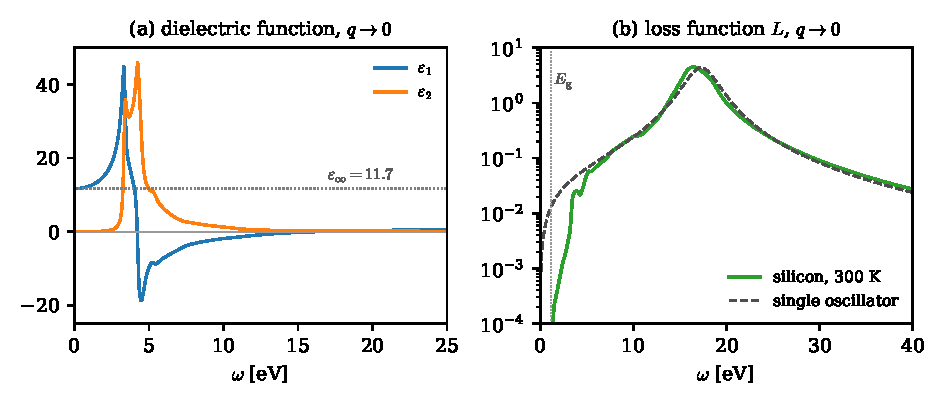
\includegraphics[width=\linewidth]{figures/ch04/fig4_5.pdf}
  \caption{Dielectric function and loss function of crystalline silicon at $q \to 0$ and \SI{300}{K}, from the optical constants of Franta and coworkers, a Kramers--Kronig-consistent dispersion model fitted to ellipsometric and spectrophotometric measurements and tabulated from \SI{4}{meV} to \SI{40}{eV}~\cite{franta2017temperature}. The data are optical, that is transverse; at $q \to 0$ the transverse and longitudinal functions coincide (\cref{eq:4.4-ET}), and $L = \varepsilon_2/|\varepsilon|^2$. (a) $\varepsilon_1$ and $\varepsilon_2$; at low energy $\varepsilon_1 = \varepsilon_\infty = 11.7$ (dotted). The interband peaks of $\varepsilon_2$ lie at 3.4 and \SI{4.2}{eV}, and $\varepsilon_1$ crosses zero upward at \SI{16.3}{eV}. (b) The loss function on a logarithmic scale (solid), with its peak of 4.5 at \SI{16.4}{eV}. Dashed: the single damped oscillator of \cref{we:4-oscillatorL} at $q = 0$, which has the same f-sum and the same $\varepsilon_\infty$, and a damping equal to the measured full width, \SI{3.66}{eV}. Dotted: the room-temperature gap, \SI{1.12}{eV}, to match the data. Below \SI{40}{eV} the tabulated spectrum collects 96 percent of the f-sum of the four valence electrons in $\int\omega\varepsilon_2\,\dd\omega$ and 92 percent in $\int\omega L\,\dd\omega$.}
  \label{fig:4-siloss}
\end{figure}

\subsection{Sum rules for the loss function}

The sum rules of \cref{sec:4.3} carry over. For the f-sum we start from its form at any temperature, $\int_0^\infty\dd\omega\,\omega(1 - \ee^{-\beta\omega})S = \pi\nd_eq^2/m_e$, which folds the negative frequencies onto the positive ones with detailed balance. By \cref{eq:4.4-SL} the factor $(1 - \ee^{-\beta\omega})S$ is $(2q^2/e^2)L$, the temperature drops out, and with $\omega_p^2 = e^2\nd_e/m_e$ from \cref{eq:4.3-wp},
\begin{equation}
  \int_0^\infty\dd\omega\;\omega\,L(\vect{q},\omega) = \frac{\pi}{2}\,\omega_p^2 ,
  \label{eq:4.4-fsumL}
\end{equation}
at every $\vect{q}$ and temperature, with $L$ for the electron channel, or the total one at clamped nuclei. This is \cref{eq:A.7-fsumL} and Ref.~\cite[Eq.~(S.10)]{hochberg2021determining}. With moving nuclei the total-charge $L$ collects in addition the nuclear share of the charge f-sum of \cref{sec:4.3}, $2.73\times10^{-4}$ of the total for silicon.

The absorptive part obeys the same rule. The macroscopic $\varepsilon_2$ is $-v_{\mathrm{C}}(q)\Imag\bar R_{\vect{0}\vect{0}}$ (\cref{app:D.7}), and $\bar R$ is the density response of the electrons with the Coulomb kernel at the single wavevector $\vect{q}$ removed from the Hamiltonian. Removing one Fourier component out of a continuum of them changes the equilibrium state by nothing in the thermodynamic limit (\cref{sec:4.8-removal}), while the double commutator of \cref{sec:4.3} does not involve the interaction at all. The response $\bar R$ therefore has the same f-sum as $R$, and
\begin{equation}
  \int_0^\infty\dd\omega\;\omega\,\varepsilon_2(\vect{q},\omega) = \frac{\pi}{2}\,\omega_p^2 ,
  \label{eq:4.4-fsumeps}
\end{equation}
which \cref{app:C.5} also obtains from the Kramers--Kronig relation for $\varepsilon - 1$ at large frequency. The two functions $\varepsilon_2$ and $L$ distribute the same weight differently: $\varepsilon_2$ puts it at the transition energies, and $L = \varepsilon_2/|\varepsilon|^2$ moves it up to where $|\varepsilon|$ is small, toward the plasmon. Tested on the tabulated silicon data of \cref{fig:4-siloss}, the spectrum below \SI{40}{eV} holds 96 percent of $(\pi/2)\omega_p^2 = \SI{433}{eV^2}$ for the four valence electrons in $\int\omega\varepsilon_2$, and 92 percent in $\int\omega L$, which has more of its weight at high energy. The rest lies above the table, where the valence absorption overlaps that of the core (\cref{we:4-sifsum}).

The inverse moments follow from the Kramers--Kronig relations at $\omega = 0$ (\cref{eq:C.5-screening,eq:C.5-KKeps}). For an insulator at $\vect{q} \to 0$,
\begin{equation}
  \frac{2}{\pi}\int_0^\infty\dd\omega\;\frac{L(\omega)}{\omega} = 1 - \frac{1}{\varepsilon_\infty}, \qquad
  \frac{2}{\pi}\int_0^\infty\dd\omega\;\frac{\varepsilon_2(\omega)}{\omega} = \varepsilon_\infty - 1 .
  \label{eq:4.4-inverse}
\end{equation}
In a metal static screening is perfect at long wavelength, $\varepsilon^{-1} \to 0$, and the first integral becomes $\pi/2$ (\cref{app:C.5}). Weighted by $1/\omega$, these integrals converge much faster than the f-sum: the tabulated data of \cref{fig:4-siloss} return 99.8 percent of $\varepsilon_\infty - 1$ and 97.8 percent of $1 - 1/\varepsilon_\infty$ below \SI{40}{eV}.

Together, the f-sum and the inverse moment already say where the weight of $L$ sits at small $q$. Their ratio defines a mean excitation energy, $\bar E^2 = \int\omega L/\int(L/\omega)$, and
\begin{equation}
  \bar E^2 = \frac{\omega_p^2}{1 - 1/\varepsilon_\infty} .
  \label{eq:4.4-Ebar}
\end{equation}
With $\omega_p = \SI{16.6}{eV}$ for the valence electrons and $\varepsilon_\infty = 11.7$, $\bar E = 16.6/0.956 = \SI{17.4}{eV}$. If the loss spectrum were a single line, it would sit there, more than fifteen times above the gap of \SI{1.17}{eV}. By \cref{eq:4.4-SL}, the same holds for the density fluctuations $S$ at $T = 0$: at long wavelengths the valence electrons respond collectively, at energies $\sim\omega_p$, and not at the gap, a point \cref{sec:4.5} makes precise.

\subsection{Optical conductivity and transverse response}

Light, and a dark photon absorbed at rest, act through a transverse field, not a potential, and what the experiment measures is a current. The induced current density $\vect{J}$ is linear in the total field $\vect{E}$, $\vect{J} = \sigma_{\mathrm{cond}}\vect{E}$, which defines the optical conductivity $\sigma_{\mathrm{cond}}(\omega) = \sigma_1 + \ii\sigma_2$. With fields varying as $\ee^{-\ii\omega t}$ (\cref{app:A.3}), the Amp\`ere--Maxwell law in Heaviside--Lorentz units, $\nabla\times\vect{B} = \vect{J} + \partial_t\vect{E}$, written as $\nabla\times\vect{B} = \partial_t\vect{D}$ with $\vect{D} = \varepsilon\vect{E}$, requires $-\ii\omega\varepsilon = \sigma_{\mathrm{cond}} - \ii\omega$, so
\begin{equation}
  \varepsilon = 1 + \frac{\ii\,\sigma_{\mathrm{cond}}}{\omega}, \qquad \sigma_1 = \omega\,\varepsilon_2, \qquad \sigma_2 = \omega\,(1 - \varepsilon_1) .
  \label{eq:4.4-sigma}
\end{equation}
Texts in Gaussian units write $\varepsilon = 1 + 4\pi\ii\sigma_{\mathrm{cond}}/\omega$ (\cref{app:A.2}). The real part $\sigma_1$ is the dissipative one, and by \cref{eq:4.4-fsumeps} it obeys $\int_0^\infty\dd\omega\,\sigma_1 = (\pi/2)\omega_p^2$, the f-sum rule in its optical form. Written with the loss function, $\sigma_1 = \omega|\varepsilon|^2L$~\cite{hochberg2021determining}. For the absorption of a dark photon, the in-medium photon self-energy of \cref{sec:1.4} is $\Pi_{\mathrm{em}} = \omega^2(1 - \varepsilon^{\mathrm{T}}) = -\ii\omega\sigma_{\mathrm{cond}}$: the wave equation $\omega^2\varepsilon^{\mathrm{T}}\vect{A} = k^2\vect{A}$ for a transverse vector potential in the medium is $(\omega^2 - k^2 - \Pi_{\mathrm{em}})\vect{A} = 0$. Its imaginary part, $-\omega\sigma_1$, sets the absorption rate of \cref{eq:1.4-absorption}.

The function that enters here is the transverse dielectric function $\varepsilon^{\mathrm{T}}$, the response to a field perpendicular to $\vect{q}$, while \cref{eq:4.4-eps} defines the longitudinal one. Both come from one tensor. A vector potential $\vect{A}\,\ee^{\ii\vect{q}\cdot\vect{r}}$ in the gauge with no scalar potential, $\vect{E} = -\partial_t\vect{A} = \ii\omega\vect{A}$, enters the kinetic energy of each electron as $(\vect{p} + e\vect{A})^2/2m_e$. To first order it couples to the paramagnetic current $\vect{j}_e(\vect{q})$ of \cref{eq:4.3-continuity} through $e\vect{A}\cdot\vect{j}_e(\vect{q})$, and it changes the velocity of every electron from $\vect{p}/m_e$ to $(\vect{p} + e\vect{A})/m_e$. The induced particle current per volume therefore has two parts. The diamagnetic part is the density times the added velocity, $\nd_e\,e\vect{A}/m_e$. The paramagnetic part is the Kubo response \cref{eq:4.1-kubo} of $\vect{j}_e$ to the perturbation $O_b\phi_{\mathrm{ext}} = j_e^\beta(\vect{q})\,eA^\beta$, which is $\tilde R^{\alpha\beta}_{jj}\,eA^\beta$, with $\tilde R^{\alpha\beta}_{jj}$ the proper current--current response, proper because $\vect{E}$ is the total field. Together,
\begin{equation*}
  \frac{\delta\langle j_e^\alpha(\vect{q})^\dagger\rangle}{\Vol} + \nd_e\frac{eA^\alpha}{m_e} = e\Bigl[\frac{\nd_e}{m_e}\delta^{\alpha\beta} + \tilde R^{\alpha\beta}_{jj}(\vect{q},\omega)\Bigr]A^\beta .
\end{equation*} Multiplying by the electron charge $-e$ and inserting $\vect{A} = -\ii\vect{E}/\omega$,
\begin{equation*}
  \varepsilon^{\alpha\beta}(\vect{q},\omega) = \delta^{\alpha\beta} - \frac{e^2}{\omega^2}\Bigl[\frac{\nd_e}{m_e}\delta^{\alpha\beta} + \tilde R^{\alpha\beta}_{jj}(\vect{q},\omega)\Bigr] .
\end{equation*}
For free electrons $\tilde R_{jj}$ vanishes at $\vect{q} = 0$, since the total momentum is conserved, and $\varepsilon = 1 - \omega_p^2/\omega^2$. The transverse function is $\varepsilon^{\mathrm{T}} = \hat{\vect{e}}\cdot\varepsilon\cdot\hat{\vect{e}}$ for a unit vector $\hat{\vect{e}} \perp \vect{q}$, and the longitudinal one is $\hat{\vect{q}}\cdot\varepsilon\cdot\hat{\vect{q}}$.

That the longitudinal projection is the $\varepsilon$ of \cref{eq:4.4-eps} follows from the continuity equation \cref{eq:4.3-continuity}, $\partial_tn_e(\vect{q},t) = \ii\vect{q}\cdot\vect{j}_e(\vect{q},t)$. In the Kubo integral for $R_{ee}(\vect{q},\omega)$ we integrate by parts in $t$ twice, using $\omega + \ii0^+$ so that the boundary terms at large $t$ vanish. The first boundary term contains the equal-time commutator of two densities, which is zero. The first integration replaces $n_e(\vect{q},t)^\dagger$ by $-\ii\vect{q}\cdot\vect{j}_e(\vect{q},t)^\dagger$; the second, after moving the time to the other operator by stationarity, replaces $n_e(\vect{q},0)$ by $\ii\vect{q}\cdot\vect{j}_e(\vect{q},0)$ and leaves the boundary term $\langle[\vect{q}\cdot\vect{j}_e^\dagger, n_e]\rangle/\Vol = \nd_eq^2/m_e$, the double commutator of the f-sum rule. The result is a Ward identity, the statement of charge conservation for the response functions,
\begin{equation}
  \omega^2R_{ee}(\vect{q},\omega) = \frac{\nd_eq^2}{m_e} + q_\alpha q_\beta\,R^{\alpha\beta}_{jj}(\vect{q},\omega) ,
  \label{eq:4.4-ward}
\end{equation}
exactly, and the same identity holds for the proper functions, by the argument that gave \cref{eq:4.4-fsumeps}~\cite[Chap.~3]{giuliani2005quantum}. Inserted into the tensor, $\hat{\vect{q}}\cdot\varepsilon\cdot\hat{\vect{q}} = 1 - (e^2/q^2)\tilde R_{ee} = \varepsilon$. As $\vect{q} \to 0$, the proper tensor $\tilde R_{jj}^{\alpha\beta}$ tends to a limit that does not depend on the direction of $\vect{q}$, since the proper response has no long-range Coulomb kernel and so no singularity at $\vect{q} = 0$. Both projections are then taken of the same tensor $\varepsilon^{\alpha\beta}(\omega)$. In a cubic crystal that tensor is a multiple of the unit matrix (\cref{app:C.3}), and
\begin{equation}
  \varepsilon^{\mathrm{T}}(\vect{q},\omega) \to \varepsilon(\vect{q},\omega) \qquad (\vect{q} \to 0) .
  \label{eq:4.4-ET}
\end{equation}
In a crystal of lower symmetry the longitudinal function depends on the direction $\hat{\vect{q}}$ even at $\vect{q} \to 0$, but it is still the projection of the optical tensor. This is why optical data at $q \to 0$ give the longitudinal loss function, as in \cref{fig:4-siloss}, and why the absorption of a dark photon and the scattering of dark matter at small $q$ are governed by the same $\varepsilon_2$. At finite $q$ the two functions separate; for dark-matter scattering, which needs momentum transfers of keV, the longitudinal function is the one that matters.

\subsection{Thomas--Fermi screening}

The simplest proper response is that of a gas of electrons in a static potential that varies slowly in space. Each region of the gas then sits in local equilibrium, with the potential energy $\phi_{\mathrm{tot}}(\vect{r})$ shifting all its levels. The electrochemical potential must be the same everywhere, so the local chemical potential is $\mu_{\mathrm{ch}} - \phi_{\mathrm{tot}}(\vect{r})$, and the density changes by $\delta\nd_e = -(\partial\nd_e/\partial\mu_{\mathrm{ch}})\,\phi_{\mathrm{tot}}$. For the free gas, $\partial\nd_e/\partial\mu_{\mathrm{ch}} = 2\mathcal{N}_{\mathrm{F}}$ at $T = 0$, with $\mathcal{N}_{\mathrm{F}}$ per spin from \cref{eq:2.5-fermi}. The proper response is $\tilde R_{ee}(q, 0) = -2\mathcal{N}_{\mathrm{F}}$, and \cref{eq:4.4-eps} gives
\begin{equation}
  \varepsilon_{\mathrm{TF}}(q) = 1 + \frac{k_{\mathrm{TF}}^2}{q^2}, \qquad
  k_{\mathrm{TF}}^2 = 2e^2\mathcal{N}_{\mathrm{F}} = \frac{4\alpha\,m_ek_{\mathrm{F}}}{\pi} = \frac{3\,\omega_p^2}{v_{\mathrm{F}}^2} ,
  \label{eq:4.4-TF}
\end{equation}
where the last two forms use \cref{eq:2.5-fermi,eq:4.3-wp}. The statically screened interaction is
\begin{equation*}
  \frac{v_{\mathrm{C}}(q)}{\varepsilon_{\mathrm{TF}}(q)} = \frac{e^2}{q^2 + k_{\mathrm{TF}}^2} ,
\end{equation*}
the transform of a Yukawa potential $\alpha\,\ee^{-k_{\mathrm{TF}}r}/r$, the same form as a massive mediator (\cref{eq:1.4-yukawa}) with mass $k_{\mathrm{TF}}$. An impurity charge in a metal is screened within a distance $1/k_{\mathrm{TF}}$. This is the Thomas--Fermi theory of screening, after the semiclassical model of the atom by Thomas and Fermi. Its assumptions are a static potential and a slow variation, $q \ll k_{\mathrm{F}}$, so that the local-equilibrium picture holds; \cref{sec:4.5} recovers \cref{eq:4.4-TF} as the static long-wavelength limit of the Lindhard function and gives the corrections.

\begin{workedexample}{The Thomas--Fermi length of the silicon valence electrons}\label{we:4-tf}
Treat the four valence electrons per atom of silicon as a free gas, $\nd_e = \SI{2.00e23}{cm^{-3}}$, with $k_{\mathrm{F}} = \SI{3.57}{keV}$ and $\mathcal{N}_{\mathrm{F}} = \SI{9.2e7}{eV^2}$ (\cref{sec:2.5}). By \cref{eq:4.4-TF}, $k_{\mathrm{TF}}^2 = 4\alpha m_ek_{\mathrm{F}}/\pi = \SI{1.69e7}{eV^2}$, or $k_{\mathrm{TF}} = \SI{4.12}{keV}$, and a screening length $1/k_{\mathrm{TF}} = \SI{0.48}{\angstrom}$, a fifth of the bond length. At the typical momentum transfer $q_0 = \alpha m_e = \SI{3.73}{keV}$, $\varepsilon_{\mathrm{TF}} = 1 + (4.12/3.73)^2 = 2.22$, and the squared potential, which sets the rate, is reduced by $|\varepsilon_{\mathrm{TF}}|^2 = 4.9$.

The estimate is crude because $k_{\mathrm{TF}}$ is not small against $k_{\mathrm{F}}$ and because silicon is an insulator. With $k_{\mathrm{TF}} = 1.15\,k_{\mathrm{F}}$, the screening happens at the wavevectors where the condition $q \ll k_{\mathrm{F}}$ fails, and the Lindhard function of \cref{sec:4.5} screens less than \cref{eq:4.4-TF} at $q \sim k_{\mathrm{F}}$. In an insulator, moreover, the electrons cannot follow a potential that varies over many cells, and its static screening at long wavelength saturates at $\varepsilon_\infty = 11.7$, while the gas formula diverges. The two descriptions meet where $1 + k_{\mathrm{TF}}^2/q^2 = \varepsilon_\infty$, at $q = k_{\mathrm{TF}}/(\varepsilon_\infty - 1)^{1/2} = \SI{1.26}{keV}$, a length $1/q$ of \SI{1.6}{\angstrom}. As a rough picture, then, silicon screens like a metal at the momentum transfers of a few keV that dark matter typically deposits, and like an insulator with a dielectric constant of 11.7 below about \SI{1}{keV}. Both statements concern the static response; the rate needs $\varepsilon$ at the energy deposited, which is why the computed loss function, not \cref{eq:4.4-TF}, enters the calculations of \cref{chap:10}.
\end{workedexample}

\subsection{Dielectric stopping}

A charged particle crossing a solid slows down by exciting it, and the loss function fixes how fast. Take a particle of charge $Z_1e$, heavy enough that its recoil can be neglected, moving with velocity $\vect{v}$. Its potential energy with an electron is $-Z_1e^2/(4\pi r)$, so $\tilde V(\vect{q}) = -Z_1v_{\mathrm{C}}(q)$, and a momentum transfer $\vect{q}$ deposits $\omega = \vect{q}\cdot\vect{v}$, the energy change $\vect{q}\cdot\vect{v} - q^2/2M_1$ of a particle of mass $M_1 \to \infty$. Weighting each momentum transfer in the rate \cref{eq:4.2-rate} by the energy it deposits gives the energy lost per unit time, and dividing by $v$ the energy lost per unit path. At $T = 0$, with \cref{eq:4.4-SL} and $|\tilde V|^2 = Z_1^2e^4/q^4$,
\begin{equation*}
  -\frac{\dd E}{\dd x} = \frac{1}{v}\int\frac{\dd^3q}{(2\pi)^3}\,\frac{Z_1^2e^4}{q^4}\,\frac{2q^2}{e^2}\,\omega\,L(\vect{q},\omega)\Big|_{\omega = \vect{q}\cdot\vect{v}} .
\end{equation*}
For an isotropic $L$ we use polar coordinates about $\vect{v}$, $\dd^3q = 2\pi q^2\dd q\,\dd u$ with $u$ the cosine of the angle, and change variables from $u$ to $\omega = quv$, $\dd u = \dd\omega/(qv)$. Only $\omega > 0$ contributes at $T = 0$, and
\begin{equation}
  -\frac{\dd E}{\dd x} = \frac{Z_1^2e^2}{2\pi^2v^2}\int_0^\infty\frac{\dd q}{q}\int_0^{qv}\dd\omega\;\omega\,L(q,\omega) = \frac{2Z_1^2\alpha}{\pi v^2}\int_0^\infty\frac{\dd q}{q}\int_0^{qv}\dd\omega\;\omega\,L(q,\omega) .
  \label{eq:4.4-dEdx}
\end{equation}
This is Lindhard's dielectric formula for the stopping power~\cite{lindhard1954properties}, in Heaviside--Lorentz units. The fast and the slow limits show what it contains. For a fast particle, $qv$ reaches beyond the whole loss spectrum at all but the smallest $q$, and the inner integral is the f-sum $(\pi/2)\omega_p^2$. The stopping power is $Z_1^2\alpha\omega_p^2/v^2$ times a logarithm of the range of $q$ that contributes: the Bethe formula, set by the electron density alone. For a slow particle, $qv$ stays below the main peak, and the inner integral samples only the low-energy side of $L$, which the sum rules do not fix. The same is true of a dark-matter particle, which is a slow probe in exactly this sense.

\begin{workedexample}{A single damped oscillator}\label{we:4-oscillatorL}
The simplest loss function consistent with the f-sum and with $\varepsilon_\infty$ puts all the weight in one damped oscillator. Write
\begin{equation*}
  \varepsilon^{-1}(q,\omega) = 1 + \frac{\omega_p^2}{\omega^2 - \omega_{\mathrm{res}}^2 + \ii\varGamma_{\mathrm{w}}\omega}, \qquad
  \omega_{\mathrm{res}}(q)^2 = \bar E^2 + \Bigl(\frac{q^2}{2m_e}\Bigr)^2 ,
\end{equation*}
with a damping rate $\varGamma_{\mathrm{w}}$. The resonance frequency moves from $\bar E$ at small $q$ to the free recoil energy $q^2/2m_e$ at large $q$; this dispersion is our modeling choice, made so that the large-$q$ limit has the free-recoil center that \cref{sec:4.3} requires. The function $\varepsilon^{-1} - 1$ has the form of the damped-oscillator response of \cref{we:4-oscillator}, with $\omega_p^2$ for $2\lambda_{\mathrm{osc}}^2\omega_0$ and $\omega_{\mathrm{res}}$ for $\omega_0$. It is causal, and its imaginary part is
\begin{equation*}
  L(q,\omega) = \frac{\omega_p^2\,\varGamma_{\mathrm{w}}\,\omega}{(\omega^2 - \omega_{\mathrm{res}}^2)^2 + \varGamma_{\mathrm{w}}^2\omega^2} .
\end{equation*}
Integrating, $\int_0^\infty\omega L\,\dd\omega = (\pi/2)\omega_p^2$ for any $\varGamma_{\mathrm{w}}$ and $q$, the f-sum \cref{eq:4.4-fsumL}, and $\int_0^\infty(L/\omega)\,\dd\omega = (\pi/2)\omega_p^2/\omega_{\mathrm{res}}^2$. At $q \to 0$ the inverse moment \cref{eq:4.4-inverse} then requires $1 - 1/\varepsilon_\infty = \omega_p^2/\bar E^2$, which is \cref{eq:4.4-Ebar}: the single oscillator that satisfies both sum rules has its loss peak at the mean excitation energy, $\bar E = \SI{17.4}{eV}$ for silicon. Inverting, $\varepsilon$ itself has its resonance lower, at $(\bar E^2 - \omega_p^2)^{1/2} = \bar E/\varepsilon_\infty^{1/2} = \SI{5.08}{eV}$, and $\varepsilon(0,0) = 11.7$. We take $\varGamma_{\mathrm{w}} = \SI{3.66}{eV}$, the measured full width of the silicon loss peak, which sets the peak height $\omega_p^2/(\varGamma_{\mathrm{w}}\bar E) = 4.34$ against the measured 4.5 (\cref{fig:4-siloss}b).

By \cref{eq:4.4-SL}, the structure factor at $T = 0$ is
\begin{equation*}
  S(q,\omega) = \frac{q^2}{2\pi\alpha}\,\frac{\omega_p^2\,\varGamma_{\mathrm{w}}\,\omega}{(\omega^2 - \omega_{\mathrm{res}}^2)^2 + \varGamma_{\mathrm{w}}^2\omega^2} ,
\end{equation*}
and its first moment is $(q^2/2\pi\alpha)(\pi/2)\omega_p^2 = \pi\nd_eq^2/m_e$, the f-sum \cref{eq:4.3-fsum}. As $\varGamma_{\mathrm{w}} \to 0$, the weight collapses onto $\omega = \omega_{\mathrm{res}}$ with $\int\dd\omega\,S = \pi\nd_eq^2/(m_e\omega_{\mathrm{res}})$, and by \cref{eq:4.2-static} $S^{\mathrm{st}} = q^2/(2m_e\omega_{\mathrm{res}})$: the density fluctuations vanish as $q^2$ at small $q$, below the bound $q^2/(2m_e\Eg)$ of \cref{sec:4.3} since $\omega_{\mathrm{res}} > \Eg$.

For the stopping power of a slow particle, take $qv \ll \omega_{\mathrm{res}}$ at every $q$. Since $\omega_{\mathrm{res}}/q$ is smallest, $(\bar E/m_e)^{1/2} = 5.8\times10^{-3}$, at $q = (2m_e\bar E)^{1/2} = \SI{4.2}{keV}$, this means $v \ll 5.8\times10^{-3}$. Then $L \simeq \omega_p^2\varGamma_{\mathrm{w}}\omega/\omega_{\mathrm{res}}^4$ on the whole range of the inner integral of \cref{eq:4.4-dEdx}, which becomes $\omega_p^2\varGamma_{\mathrm{w}}q^3v^3/(3\omega_{\mathrm{res}}^4)$. With $q = (2m_e\bar E)^{1/2}x$, the remaining integral is $\int_0^\infty q^2\dd q/\omega_{\mathrm{res}}^4 = (2m_e\bar E)^{3/2}\bar E^{-4}\int_0^\infty x^2\dd x/(1 + x^4)^2$, and the last integral is $\pi/(8\sqrt2)$. Altogether
\begin{equation*}
  -\frac{\dd E}{\dd x} \simeq \frac{Z_1^2\,\alpha\,\varGamma_{\mathrm{w}}\,\omega_p^2\,m_e^{3/2}}{6\,\bar E^{5/2}}\;v .
\end{equation*}
The slow particle feels a friction proportional to its speed, with a coefficient set by the damping. For silicon's numbers and $Z_1 = 1$ it is \SI{0.18}{eV/\angstrom} at $v = 10^{-3}$; the full integral \cref{eq:4.4-dEdx} gives \SI{0.186}{eV/\angstrom}, 3 percent more, and 22 percent more at $v_{\mathrm{max}} = 2.65\times10^{-3}$, where the condition $v \ll 5.8\times10^{-3}$ is only marginal.

The coefficient tests only the tail of the model. The energies that matter are up to $qv \approx \SI{4}{eV}$ at the dominant $q \approx \SI{4}{keV}$, and there the oscillator and silicon disagree badly: at \SI{3}{eV} the model has $L = 0.035$, eleven times the measured value, and it has weight below the gap, where silicon has none (\cref{fig:4-siloss}b). Both loss functions satisfy the f-sum and give the same $\varepsilon_\infty$. The sum rules fix the main peak, while slow particles, and dark matter, sample the low-energy side of $L$, which only a calculation or a measurement of the actual material can supply.
\end{workedexample}

\section{The homogeneous electron gas}\label{sec:4.5}

Spread the four valence electrons of each silicon atom uniformly over the crystal, replace the ions by a uniform positive background, and ask where the loss function of this electron gas peaks at long wavelength. The answer is the plasma frequency, $\omega_p = \SI{16.6}{eV}$, and the measured loss peak of silicon in \cref{fig:4-siloss} lies at \SI{16.4}{eV}. A model with no lattice, no gap and no bonds places the main feature of the spectrum within 1.2 percent of the measured peak. The reason is that at long wavelength and high frequency the valence electrons respond collectively, and the details of the crystal matter less than the Coulomb force between them. The electron gas is also the one interacting system in which the independent-particle response and its screened version can be written in closed form, and this is why it serves as the reference model for valence electrons, plasmons and screening.

The model is jellium (\cref{we:2-jellium}) at the valence density of silicon, $\nd_e = \SI{2.00e23}{cm^{-3}}$. Its density parameter, the radius per electron in units of the Bohr radius, is $r_s = 2.0$ (\cref{sec:2.3}), and the free-gas scales of \cref{eq:2.5-fermi} are $k_{\mathrm{F}} = \SI{3.57}{keV}$, $E_{\mathrm{F}} = \SI{12.5}{eV}$ and $v_{\mathrm{F}} = 7.0\times10^{-3}$. In these units the plasma frequency is $\omega_p = 1.33\,E_{\mathrm{F}}$ and the Thomas--Fermi wavevector of \cref{eq:4.4-TF} is $k_{\mathrm{TF}} = 1.15\,k_{\mathrm{F}}$. Both ratios grow with $r_s$, since $k_{\mathrm{TF}}^2/k_{\mathrm{F}}^2 = 4\alpha m_e/(\pi k_{\mathrm{F}}) = 0.663\,r_s$ with $k_{\mathrm{F}} = (9\pi/4)^{1/3}/(r_sa_0)$: the denser the gas, the weaker the Coulomb force compared with the kinetic energy.

\subsection{The independent-particle bubble}

Without the Coulomb interaction the electrons of jellium are free, and the Lehmann representation \cref{eq:4.1-lehmann} of their density response is a sum over the moves of one electron. Take an occupation-number state $|i\rangle$ of plane waves, with the spin included in the label $\vect{k}$. The operator $n_e(\vect{q}) = \sum_{\vect{k}}c^\dagger_{\vect{k}+\vect{q}}c_{\vect{k}}$ of \cref{eq:2.3-nq} moves one electron from $\vect{k}$ to $\vect{k} + \vect{q}$, and the move is possible only if $\vect{k}$ is occupied and $\vect{k} + \vect{q}$ empty. In the resonant term of \cref{eq:4.1-lehmann} the final state $|f\rangle$ is this move, with weight $n_{\vect{k}}(1 - n_{\vect{k}+\vect{q}})$ and energy $E_f - E_i = \xi_{\vect{k}+\vect{q}} - \xi_{\vect{k}}$. In the antiresonant term $n_e(\vect{q})^\dagger$ makes the reverse move, from $\vect{k} + \vect{q}$ to $\vect{k}$, with weight $n_{\vect{k}+\vect{q}}(1 - n_{\vect{k}})$ and energy $\xi_{\vect{k}} - \xi_{\vect{k}+\vect{q}}$. The two terms then share the denominator $\omega + \xi_{\vect{k}} - \xi_{\vect{k}+\vect{q}} + \ii0^+$, and their numerators combine to $n_{\vect{k}}(1 - n_{\vect{k}+\vect{q}}) - n_{\vect{k}+\vect{q}}(1 - n_{\vect{k}}) = n_{\vect{k}} - n_{\vect{k}+\vect{q}}$. The Pauli factors have cancelled: a move into an occupied state appears in both terms with opposite signs. The thermal average of $n_{\vect{k}}$ over the Gibbs state is $n_{\mathrm{F}}(\xi_{\vect{k}})$, and
\begin{equation}
  R^0(\vect{q},\omega) = \frac{1}{\Vol}\sum_{\vect{k}}\frac{n_{\mathrm{F}}(\xi_{\vect{k}}) - n_{\mathrm{F}}(\xi_{\vect{k}+\vect{q}})}{\omega + \xi_{\vect{k}} - \xi_{\vect{k}+\vect{q}} + \ii0^+} ,
  \label{eq:4.5-R0}
\end{equation}
the independent-particle bubble. This is the Matsubara bubble \cref{eq:4.7-bubble} continued to real frequencies, obtained here without imaginary time. Its imaginary part counts the transitions of \cref{eq:2.5-indep}, and by the fluctuation--dissipation theorem it is $-\tfrac12S^0$ at $T = 0$, with the structure factor of \cref{we:4-gas}.

At $T = 0$ the sum is a set of elementary integrals over the Fermi sphere, which \cref{app:D.8} carries out for any complex frequency $z$ in the upper half plane. The result is the Lindhard function~\cite{lindhard1954properties}.
\begin{keyresult}[Lindhard function]
\begin{equation}
  R^0(q,\omega) = -2\mathcal{N}_{\mathrm{F}}\left\{\frac12 + \frac{k_{\mathrm{F}}}{4q}\Bigl[(1 - \nu_+^2)\,\ell(\nu_+) - (1 - \nu_-^2)\,\ell(\nu_-)\Bigr]\right\} ,
  \label{eq:4.5-lindhard}
\end{equation}
with $\nu_\pm = (\omega + \ii0^+)/qv_{\mathrm{F}} \pm q/2k_{\mathrm{F}}$, $\ell(w) = \ln[(w + 1)/(w - 1)]$ on the principal branch and $\mathcal{N}_{\mathrm{F}} = m_ek_{\mathrm{F}}/2\pi^2$ per spin. It is \cref{eq:D.8-Rz} at $z = \omega + \ii0^+$, and it holds with $\omega + \ii0^+$ replaced by any $z$ with $\Imag z > 0$.
\end{keyresult}
Apart from the prefactor $2\mathcal{N}_{\mathrm{F}}$, the response depends on two numbers only, the momentum in units of the diameter of the Fermi sphere, $y = q/2k_{\mathrm{F}}$, and the frequency in units of the largest Doppler shift, $\omega/qv_{\mathrm{F}}$. On the real axis the logarithms take the branch \cref{eq:C.8-branch}, $\ell(\nu + \ii0^+) = \ln|(\nu + 1)/(\nu - 1)| - \ii\pi\,\Theta(1 - |\nu|)$. The real part, \cref{eq:D.8-Re}, keeps the form of \cref{eq:4.5-lindhard} with the logarithms of the moduli. The imaginary part is a sum of steps, and it is nonzero only between the edges
\begin{equation*}
  \omega_+ = qv_{\mathrm{F}} + \frac{q^2}{2m_e}, \qquad \omega_- = \max\Bigl(0,\ \frac{q^2}{2m_e} - qv_{\mathrm{F}}\Bigr) ,
\end{equation*}
the particle--hole continuum of \cref{fig:4-gas}. Inside it, \cref{eq:D.8-Im} is $-\tfrac12$ times the linear and parabolic forms of $S^0$ found by counting transitions in \cref{we:4-gas}, as the fluctuation--dissipation theorem requires. The real part, which counts the same transitions off resonance through their principal values, is the new information.

The static limit and the high-frequency tail of the real part are needed below. At $\omega = 0$ (\cref{app:D.8}),
\begin{equation}
  R^0(q,0) = -2\mathcal{N}_{\mathrm{F}}\,F_{\mathrm{L}}\Bigl(\frac{q}{2k_{\mathrm{F}}}\Bigr), \qquad
  F_{\mathrm{L}}(y) = \frac12 + \frac{1 - y^2}{4y}\ln\Bigl|\frac{1 + y}{1 - y}\Bigr| ,
  \label{eq:4.5-static}
\end{equation}
with the function $F_{\mathrm{L}}$ of \cref{eq:C.8-FL}, which falls from one at $q = 0$ to $\tfrac12$ at $q = 2k_{\mathrm{F}}$ and decays as $4k_{\mathrm{F}}^2/(3q^2)$ at large $q$. At high frequency it is simplest to start again from the sum. Let $\Delta_{\vect{k}} = q^2/2m_e + kqu/m_e$ be the energy of the move, with $u$ the cosine of the angle between $\vect{k}$ and $\vect{q}$, and let $\langle\cdot\rangle$ be the average over the Fermi sphere. Relabeling $\vect{k} \to -\vect{k} - \vect{q}$ in the term with $n_{\vect{k}+\vect{q}}$, as \cref{app:D.8} does, puts \cref{eq:4.5-R0} at $T = 0$ in the form $R^0 = \nd_e\langle 2\Delta_{\vect{k}}/(z^2 - \Delta_{\vect{k}}^2)\rangle$. For $|z| > \omega_+$, the largest $|\Delta_{\vect{k}}|$, the geometric series converges,
\begin{equation}
  R^0(q,z) = \frac{2\nd_e}{z^2}\sum_{j=0}^\infty\frac{\langle\Delta_{\vect{k}}^{2j+1}\rangle}{z^{2j}}
  = \frac{\nd_eq^2}{m_ez^2}\left[1 + \frac{\tfrac35q^2v_{\mathrm{F}}^2 + (q^2/2m_e)^2}{z^2} + \frac{\tfrac37q^4v_{\mathrm{F}}^4 + O(q^6)}{z^4} + O(z^{-6})\right] .
  \label{eq:4.5-moments}
\end{equation}
The averages are elementary. Odd powers of $u$ vanish, and $\langle k^2u^2\rangle = \tfrac15k_{\mathrm{F}}^2$ and $\langle k^4u^4\rangle = \tfrac{3}{35}k_{\mathrm{F}}^4$ from $\langle k^{2n}\rangle = 3k_{\mathrm{F}}^{2n}/(2n + 3)$ and $\langle u^{2n}\rangle = 1/(2n + 1)$. Hence $\langle\Delta\rangle = q^2/2m_e$, $\langle\Delta^3\rangle = (q^2/2m_e)[(q^2/2m_e)^2 + \tfrac35q^2v_{\mathrm{F}}^2]$ and $\langle\Delta^5\rangle = (q^2/2m_e)[\tfrac37q^4v_{\mathrm{F}}^4 + O(q^6)]$. The leading term is the free-particle tail whose coefficient is the f-sum. The coefficients are the odd moments of the energies of the moves, the frequency moments of $S^0$ of \cref{sec:4.3}.

The crystal bubble of \cref{sec:4.6} is computed on a grid of $\vect{k}$ points, over a finite number of bands and with a broadening in place of $\ii0^+$. The closed form \cref{eq:4.5-lindhard} has no such parameters, and the gas is the standard test of the codes that compute it.

\subsection{The random-phase approximation}

The Coulomb interaction enters through the proper response of \cref{sec:4.4}. The random-phase approximation replaces it by the independent-particle bubble,
\begin{equation}
  \tilde R_{ee} \simeq R^0, \qquad
  \varepsilon_{\mathrm{Lin}}(q,\omega) = 1 - v_{\mathrm{C}}(q)\,R^0(q,\omega), \qquad
  R_{ee} = \frac{R^0}{\varepsilon_{\mathrm{Lin}}} ,
  \label{eq:4.5-rpa}
\end{equation}
by \cref{eq:4.4-eps,eq:4.4-dyson}, and $\varepsilon_{\mathrm{Lin}}$ with $R^0$ of \cref{eq:4.5-lindhard} is the Lindhard dielectric function. In this approximation each electron responds as a free particle to the total potential, external plus Hartree, and to nothing else. It drops the hole that exchange and correlation dig around each electron, which makes the potential an electron feels differ from the average Hartree potential; \cref{sec:4.6} puts it back as an exchange--correlation kernel. The name goes back to Bohm and Pines, who derived the collective oscillation from the equation of motion of $n_e(\vect{q})$ by dropping the terms that couple it to density fluctuations at other wavevectors, on the argument that their phases are random and average out~\cite{bohm1953collective}. The approximation is exact to leading order at high density, $r_s \ll 1$, where the kinetic energy dominates and the correlation hole matters least. At $r_s = 2$ it still holds at long wavelength, since at small $q$ the Hartree term $v_{\mathrm{C}}R^0 \propto 1/q^2$ dominates every correction.

In the static limit the random-phase approximation screens a slowly varying potential exactly as Thomas--Fermi theory does, and it corrects that theory at shorter wavelengths. By \cref{eq:4.5-static} and $k_{\mathrm{TF}}^2 = 2e^2\mathcal{N}_{\mathrm{F}}$,
\begin{equation*}
  \varepsilon_{\mathrm{Lin}}(q,0) = 1 + \frac{k_{\mathrm{TF}}^2}{q^2}\,F_{\mathrm{L}}\Bigl(\frac{q}{2k_{\mathrm{F}}}\Bigr) ,
\end{equation*}
and $F_{\mathrm{L}} = 1 - q^2/12k_{\mathrm{F}}^2 + O(q^4)$ recovers \cref{eq:4.4-TF} at $q \ll k_{\mathrm{F}}$. As the wavelength shrinks to the spacing of the electrons, the gas screens less than the local-equilibrium picture of \cref{sec:4.4} assumes, because a potential that varies on the scale $1/k_{\mathrm{F}}$ cannot be followed by a shift of the local Fermi level. At the silicon valence density and the typical momentum transfer $q_0 = \SI{3.73}{keV}$, $\varepsilon_{\mathrm{Lin}}(q_0, 0) = 2.10$ against $\varepsilon_{\mathrm{TF}} = 2.22$, and the screening factor $1/|\varepsilon|^2$ of the static potential is $1/4.41$ rather than $1/4.9$ (\cref{we:4-tf}). At $q = 2k_{\mathrm{F}}$, the momentum that spans the Fermi sphere, $F_{\mathrm{L}}$ has a logarithmic kink (\cref{app:C.8}). In position space it turns the screening cloud around an impurity into a damped oscillation at the wavevector $2k_{\mathrm{F}}$, the Friedel oscillation; in the lattice dynamics of a metal the same kink is the Kohn anomaly.

\begin{limitbox}[Thomas--Fermi screening][lim:4.5a]
A static potential that varies slowly in an electron gas is screened by the dielectric function $\varepsilon_{\mathrm{TF}} = 1 + k_{\mathrm{TF}}^2/q^2$, with $k_{\mathrm{TF}}^2 = 3\omega_p^2/v_{\mathrm{F}}^2$~\cite[Eq.~(S.14)]{hochberg2021determining}.
\par\smallskip
{\centering
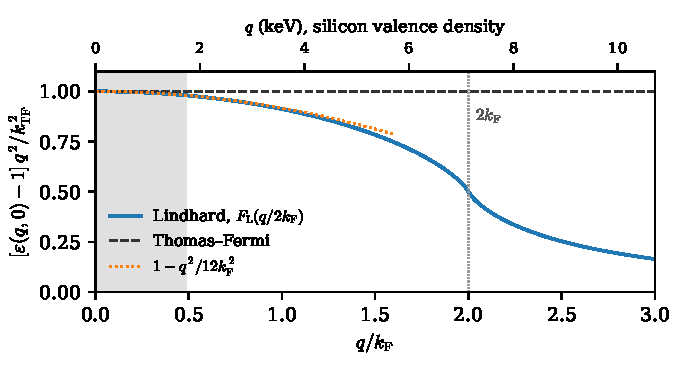
\includegraphics[width=\linewidth]{figures/ch04/limit4_tf.pdf}
\captionof{figure}{Static screening of the electron gas in the random-phase approximation against Thomas--Fermi theory. The induced part of the dielectric function, $[\varepsilon(q,0) - 1]\,q^2/k_{\mathrm{TF}}^2$, is the Lindhard function $F_{\mathrm{L}}(q/2k_{\mathrm{F}})$ (solid) and one for Thomas--Fermi (dashed); dotted, the leading correction $1 - q^2/12k_{\mathrm{F}}^2$. The curve depends on $q/k_{\mathrm{F}}$ alone; the top axis gives $q$ for the silicon valence density, $k_{\mathrm{F}} = \SI{3.57}{keV}$. Gray: $q < 0.49\,k_{\mathrm{F}}$, where the two agree within 2 percent; they differ by 10 percent at $q = 1.06\,k_{\mathrm{F}}$. The kink at $2k_{\mathrm{F}}$ is the edge of the Fermi sphere.}\label{fig:4-tf-limit}
\par}
\smallskip
At $q \gtrsim k_{\mathrm{F}}$ the local-equilibrium picture fails and the gas screens less; beyond $2k_{\mathrm{F}}$ the induced term falls as $1/q^4$ instead of $1/q^2$, and screening dies out.
\end{limitbox}

Static screening at long wavelength is perfect. As $q \to 0$, $\varepsilon_{\mathrm{Lin}}(q, 0) \to \infty$, and an external charge is completely neutralized by the charge it induces: the induced density at $q \to 0$ is $R_{ee}\phi_{\mathrm{ext}} = -(1 - 1/\varepsilon)\,\phi_{\mathrm{ext}}/v_{\mathrm{C}}$, the opposite of the external charge. Through the inverse-moment relation \cref{eq:C.5-screening} this becomes a sum rule for the loss function, $(2/\pi)\int_0^\infty\dd\omega\,L(q,\omega)/\omega = 1 - 1/\varepsilon(q, 0) \to 1$, the perfect-screening sum rule of a metal. At the silicon valence density and $q = 0.1\,k_{\mathrm{F}}$ the right side is 0.9925. In an insulator the same integral is $1 - 1/\varepsilon_\infty$ (\cref{eq:4.4-inverse}), 0.915 for silicon; the gas, with no gap, screens like a metal.

\Cref{fig:4-gasloss}a shows the loss function $L = \Imag(-1/\varepsilon_{\mathrm{Lin}})$ of the gas at $r_s = 2$ over the $(q, \omega)$ plane. Inside the particle--hole continuum, $\varepsilon_2 = -v_{\mathrm{C}}\Imag R^0$ and $L = \varepsilon_2/|\varepsilon_{\mathrm{Lin}}|^2$. At $q \gg k_{\mathrm{F}}$, where $v_{\mathrm{C}}R^0$ is small, $\varepsilon_{\mathrm{Lin}} \to 1$, and the loss function is the free-recoil parabola of \cref{we:4-gas}, centered on $q^2/2m_e$: at short wavelength the electrons scatter one at a time, and screening is irrelevant. At $q \lesssim k_{\mathrm{F}}$ the factor $1/|\varepsilon_{\mathrm{Lin}}|^2$ suppresses the continuum, and the weight moves out of it, into a line above it. Since the f-sum rule fixes the total weight at every $q$, the weight that screening removes from the pairs goes into the line.

\subsection{The plasmon}

The line is the plasma oscillation, and its frequency follows from a classical argument. Displace all the electrons of a slab of jellium by a small distance $s$ along $x$, against the fixed positive background. The two faces of the slab acquire surface charges $\pm e\nd_es$ per unit area, and between them the field, in Heaviside--Lorentz units, is $E = e\nd_es$. Each electron feels the restoring force $-eE$, and $m_e\ddot s = -e^2\nd_es$: the electrons oscillate together at $\omega_p = (e^2\nd_e/m_e)^{1/2}$, the plasma frequency of \cref{eq:4.3-wp}, whatever the size of the slab. No electron moves relative to its neighbors, and no kinetic energy of the Fermi sea enters. At finite wavelength it does, and the random-phase approximation adds it.

A pole of the response with nothing to drive it is a zero of the dielectric function, by \cref{eq:4.4-dyson}. Above the continuum, $\omega > \omega_+$, $\Imag R^0 = 0$ and $\varepsilon_{\mathrm{Lin}}$ is real, so a zero there is a pole of $1/\varepsilon_{\mathrm{Lin}}$ on the real axis, a mode that does not decay. Inserting \cref{eq:4.5-moments} into \cref{eq:4.5-rpa}, with $v_{\mathrm{C}}\nd_eq^2/m_e = \omega_p^2$,
\begin{equation*}
  \varepsilon_{\mathrm{Lin}}(q,\omega) = 1 - \frac{\omega_p^2}{\omega^2}\left[1 + \frac{A}{\omega^2} + \frac{B}{\omega^4} + \dots\right], \qquad
  A = \tfrac35q^2v_{\mathrm{F}}^2 + \Bigl(\frac{q^2}{2m_e}\Bigr)^2, \qquad B = \tfrac37q^4v_{\mathrm{F}}^4 + O(q^6) .
\end{equation*}
Setting it to zero gives $\omega^2 = \omega_p^2 + A\omega_p^2/\omega^2 + B\omega_p^2/\omega^4 + \dots$, which we solve by iteration. At zeroth order $\omega = \omega_p$. Substituting $\omega^2 = \omega_p^2 + A$ on the right, $A\omega_p^2/\omega^2 = A - A^2/\omega_p^2 + O(q^6)$ and $B\omega_p^2/\omega^4 = B/\omega_p^2 + O(q^6)$, so
\begin{keyresult}[Plasmon dispersion in the random-phase approximation]
\begin{equation}
  \omega_{\mathrm{pl}}(q)^2 = \omega_p^2 + \frac35v_{\mathrm{F}}^2q^2 + \Bigl(\frac{1}{4m_e^2} + \frac{12}{175}\,\frac{v_{\mathrm{F}}^4}{\omega_p^2}\Bigr)q^4 + O(q^6) ,
  \label{eq:4.5-dispersion}
\end{equation}
where $\tfrac{12}{175} = \tfrac37 - \tfrac{9}{25}$ collects $B$ and $-A^2$. The plasmon of the electron gas starts at $\omega_p$ and rises quadratically with $q$.
\end{keyresult}
The $q^2$ term is the pressure of the Fermi sea. A classical plasma at temperature $T$ has $3T/m_e$ in place of $\tfrac35v_{\mathrm{F}}^2$. In the degenerate gas the electrons already move at speeds up to $v_{\mathrm{F}}$ at $T = 0$, and $\tfrac35v_{\mathrm{F}}^2$ is three times their mean square velocity along $\vect{q}$, $\langle k^2u^2\rangle/m_e^2 = \tfrac15v_{\mathrm{F}}^2$. Written as $\omega_{\mathrm{pl}} \simeq \omega_p + \alpha_{\mathrm{pl}}q^2/m_e$, the dispersion coefficient is $\alpha_{\mathrm{pl}} = \tfrac35E_{\mathrm{F}}/\omega_p$, 0.45 at the silicon valence density. The expansion converges only outside the continuum, $\omega_{\mathrm{pl}} > \omega_+$, and \cref{fig:4-plasmon-limit} compares it with the exact zero of $\varepsilon_{\mathrm{Lin}}$.

\begin{limitbox}[Plasmon dispersion][lim:4.5b]
In the random-phase approximation the plasmon of an electron gas disperses as $\omega_{\mathrm{pl}}^2 \simeq \omega_p^2 + \tfrac35q^2v_{\mathrm{F}}^2$ and exists up to a cutoff $q_{\mathrm{c}} \simeq \omega_p/v_{\mathrm{F}}$~\cite[Eq.~(171) and the text following it]{kahn2022searches}.
\par\smallskip
{\centering
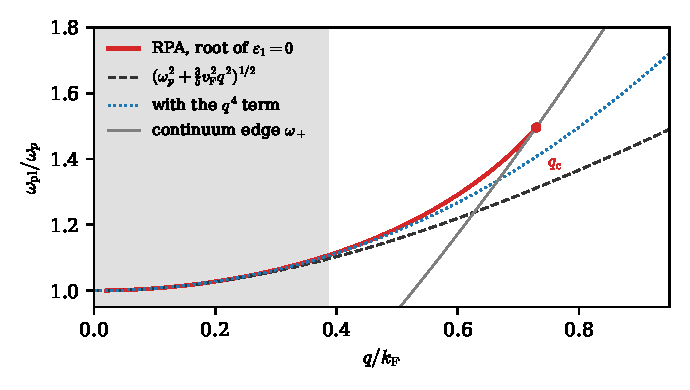
\includegraphics[width=\linewidth]{figures/ch04/limit4_plasmon.pdf}
\captionof{figure}{Plasmon dispersion of the electron gas at $r_s = 2$, the silicon valence density, in the random-phase approximation. Solid: the zero of $\Real\varepsilon_{\mathrm{Lin}}$ above the continuum, computed from \cref{eq:4.5-lindhard}, ending at $q_{\mathrm{c}} = 0.730\,k_{\mathrm{F}}$ where it meets the continuum edge $\omega_+ = qv_{\mathrm{F}} + q^2/2m_e$ (thin line). Dashed: the quadratic formula; dotted: with the $q^4$ term of \cref{eq:4.5-dispersion}. Gray: $q < 0.39\,k_{\mathrm{F}}$, where the quadratic formula is within one percent; there the $q^4$ term reduces the error to below $1.6\times10^{-3}$, and to below $3\times10^{-4}$ for $q < 0.30\,k_{\mathrm{F}}$. The estimate $q_{\mathrm{c}} \simeq \omega_p/v_{\mathrm{F}} = 0.666\,k_{\mathrm{F}}$ is 9 percent low.}\label{fig:4-plasmon-limit}
\par}
\smallskip
Near $q_{\mathrm{c}}$ the series in $q^2$ fails, since the plasmon approaches the pair energies that set its radius of convergence; beyond $q_{\mathrm{c}}$ there is no undamped plasmon.
\end{limitbox}

The weight of the plasmon follows from the slope of $\varepsilon_{\mathrm{Lin}}$ at its zero. Near $\omega_{\mathrm{pl}}$, $\varepsilon_{\mathrm{Lin}} \simeq (\partial\varepsilon_1/\partial\omega)(\omega - \omega_{\mathrm{pl}} + \ii0^+)$, with the $\ii0^+$ carried from $\omega$, and the Sokhotski--Plemelj formula gives
\begin{equation}
  L(q,\omega) = \frac{\pi}{\partial\varepsilon_1/\partial\omega|_{\omega_{\mathrm{pl}}}}\,\delta\bigl(\omega - \omega_{\mathrm{pl}}(q)\bigr) \;\to\; \frac{\pi\omega_p}{2}\,\delta(\omega - \omega_p) \qquad (q \to 0) ,
  \label{eq:4.5-plasmonL}
\end{equation}
since $\varepsilon_1 \to 1 - \omega_p^2/\omega^2$ with slope $2/\omega_p$ at $\omega_p$. At long wavelength the line alone satisfies both sum rules. Its first moment is $(\pi/2)\omega_p^2$, the whole f-sum \cref{eq:4.4-fsumL}, and its inverse moment is $\pi/2$, the whole perfect-screening rule. The continuum, whose weight vanishes as $q \to 0$, has nothing left. By \cref{eq:4.4-SL}, the structure factor at $T = 0$ is then $S = (\pi q^2\omega_p/e^2)\,\delta(\omega - \omega_p)$. Its integral over $\omega$ is $2\pi\nd_eS^{\mathrm{st}}$ by \cref{eq:4.2-static}, and with $e^2\nd_e = m_e\omega_p^2$
\begin{equation*}
  S^{\mathrm{st}}(q) \to \frac{q^2}{2m_e\omega_p} \qquad (q \to 0) .
\end{equation*}
The mean energy $q^2/(2m_eS^{\mathrm{st}})$ of \cref{sec:4.3} is $\omega_p$ at small $q$, and the density fluctuations of the interacting gas vanish as $q^2$, much faster than the $3q/4k_{\mathrm{F}}$ of the free gas. At $q = 0.1\,k_{\mathrm{F}}$ the two are $7.5\times10^{-3}$ and $7.5\times10^{-2}$. The Coulomb force suppresses long-wavelength fluctuations of the charge, since any such fluctuation costs the energy of a plasma oscillation. At finite $q$ the plasmon shares the f-sum with the continuum. Integrating the gridded loss function of \cref{fig:4-gasloss} and adding the weight of \cref{eq:4.5-plasmonL} returns $(\pi/2)\omega_p^2$ to $10^{-5}$ at $q = 0.1\,k_{\mathrm{F}}$ and $0.5\,k_{\mathrm{F}}$; the plasmon carries $1 - 4\times10^{-5}$ of it at $0.1\,k_{\mathrm{F}}$ and 0.957 at $0.5\,k_{\mathrm{F}}$.

The plasmon cannot decay as long as no electron--hole pair has its energy and momentum, that is, as long as $\omega_{\mathrm{pl}}(q) > \omega_+(q)$. The dispersion rises as $q^2$ from $\omega_p$, while the continuum edge rises linearly from zero, and the two meet at the momentum $q_{\mathrm{c}}$ defined by $\varepsilon_{\mathrm{Lin}}(q_{\mathrm{c}}, \omega_+(q_{\mathrm{c}})) = 0$. A rough estimate sets $\omega_+ \simeq qv_{\mathrm{F}}$ equal to $\omega_p$, $q_{\mathrm{c}} \simeq \omega_p/v_{\mathrm{F}}$. At $r_s = 2$ the exact root is $q_{\mathrm{c}} = 0.730\,k_{\mathrm{F}} = \SI{2.60}{keV}$, at $\omega_{\mathrm{pl}} = \SI{24.8}{eV}$; the estimate is $0.666\,k_{\mathrm{F}}$. Beyond $q_{\mathrm{c}}$, $\varepsilon_2 \ne 0$ where $\varepsilon_1$ vanishes, the zero of $\varepsilon_{\mathrm{Lin}}$ continued below the real axis moves into the lower half plane, and the plasmon becomes a resonance of the kind described in \cref{sec:4.1}, with a width that grows quickly with $q$. Its energy goes into single electron--hole pairs. This is Landau damping, named after the analogous damping of waves in a classical plasma by particles that move with the wave.

\begin{figure}[tbp]
  \centering
  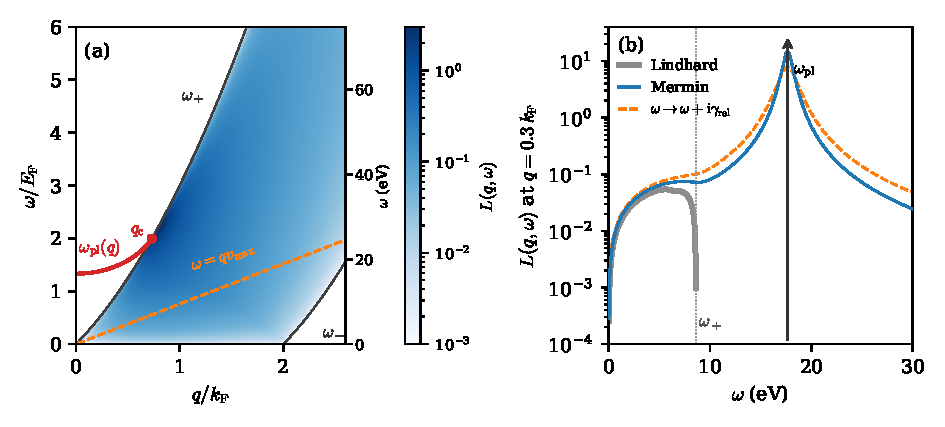
\includegraphics[width=\linewidth]{figures/ch04/fig4_6.pdf}
  \caption{Loss function of the electron gas at $r_s = 2$, the valence density of silicon ($k_{\mathrm{F}} = \SI{3.57}{keV}$, $E_{\mathrm{F}} = \SI{12.5}{eV}$, $\omega_p = \SI{16.6}{eV}$), in the random-phase approximation at $T = 0$. (a) $L(q,\omega) = \Imag[-1/\varepsilon_{\mathrm{Lin}}]$, logarithmic color scale, inside the particle--hole continuum bounded by $\omega_\pm$ (thin lines); the right axis gives $\omega$ in eV. Red: the undamped plasmon $\omega_{\mathrm{pl}}(q)$, a delta function in $L$, drawn as a line up to $q_{\mathrm{c}} = 0.730\,k_{\mathrm{F}}$ (dot), where it enters the continuum and is Landau damped. Dashed: the largest energy a dark-matter particle can deposit at momentum $q$, $\omega = qv_{\mathrm{max}}$ with $v_{\mathrm{max}} = 0.379\,v_{\mathrm{F}}$; it stays below the plasmon at every $q$. (b) $L$ at $q = 0.3\,k_{\mathrm{F}}$ on a logarithmic scale. Thick gray: Lindhard, with the continuum ending at $\omega_+$ and the plasmon as a delta function (arrow, at \SI{17.65}{eV}). Solid: the Mermin function with $\gamma_{\mathrm{rel}} = \SI{1}{eV}$, an illustrative relaxation rate. Dashed: the naive substitution $\omega \to \omega + \ii\gamma_{\mathrm{rel}}$ in $R^0$ with the same rate. Its plasmon peak is twice as wide, and its tail between the continuum and the plasmon is up to 1.7 times higher.}
  \label{fig:4-gasloss}
\end{figure}

In \cref{fig:4-gasloss}a the plasmon line enters the continuum at $q_{\mathrm{c}}$, where the loss function of the continuum is largest. From there a broad Landau-damped ridge continues toward the free-recoil parabola. Dark matter samples the low-energy corner of the continuum, where the electrons near the Fermi surface absorb the energy and the factor $1/|\varepsilon_{\mathrm{Lin}}|^2$ screens it. At small $q$ and $\omega \ll qv_{\mathrm{F}}$ the corner has a simple form. There $\varepsilon_2 = (e^2/q^2)\,m_e^2\omega/(2\pi q)$ from the linear form of $\Imag R^0$, and $\varepsilon_1 \simeq k_{\mathrm{TF}}^2/q^2 \gg \varepsilon_2$, so
\begin{equation*}
  L(q,\omega) \simeq \frac{\varepsilon_2}{\varepsilon_1^2} = \frac{e^2m_e^2}{2\pi k_{\mathrm{TF}}^4}\,q\,\omega \qquad (q \ll k_{\mathrm{F}},\ \omega \ll qv_{\mathrm{F}}) ,
\end{equation*}
linear in both $q$ and $\omega$, and suppressed by the fourth power of the screening wavevector. At the typical momentum transfer $q_0$ and the largest energy $q_0v_{\mathrm{max}} = \SI{9.88}{eV}$, the full Lindhard function yields $|\varepsilon_{\mathrm{Lin}}|^2 = 3.96$ and $L = 0.183$: dynamic screening at the energy deposited is slightly weaker than the static estimate of \cref{we:4-tf}.

\subsection{Collisions and the Mermin function}

In a real metal, or a doped semiconductor, the electrons scatter off impurities and phonons at some rate $\gamma_{\mathrm{rel}}$, and the sharp edges of the Lindhard function and its undamped plasmon are smeared on that scale. The obvious way to include the collisions is to give the frequency an imaginary part, $\omega \to \omega + \ii\gamma_{\mathrm{rel}}$, in $R^0$. This substitution is equivalent to letting the electrons relax toward the uniform equilibrium state at the rate $\gamma_{\mathrm{rel}}$. It has an unphysical consequence: the excess density at a crest of the disturbance decays at that rate even when no current flows to carry it away. Electrons are destroyed at the crests and created in the troughs. Collisions with impurities and phonons conserve the number of electrons, and they relax the shape of the distribution at each point while leaving the number of electrons there unchanged. Mermin~\cite{mermin1970lindhard} therefore let the electrons relax toward a local equilibrium that has, at each instant, the same density as the disturbed gas. \Cref{app:D.9} solves the equation of motion of the one-electron density matrix with this relaxation term and finds the response $\delta\nd_e/\phi = R^{\mathrm{Mer}}$, which in the random-phase approximation gives the Mermin dielectric function.
\begin{keyresult}[Mermin dielectric function]
\begin{equation}
  \varepsilon_{\mathrm{Mer}}(q,\omega) = 1 + \frac{(1 + \ii\gamma_{\mathrm{rel}}/\omega)\,\bigl[\varepsilon_{\mathrm{Lin}}(q,\omega + \ii\gamma_{\mathrm{rel}}) - 1\bigr]}{1 + (\ii\gamma_{\mathrm{rel}}/\omega)\,\bigl[\varepsilon_{\mathrm{Lin}}(q,\omega + \ii\gamma_{\mathrm{rel}}) - 1\bigr]/\bigl[\varepsilon_{\mathrm{Lin}}(q,0) - 1\bigr]} ,
  \label{eq:4.5-mermin}
\end{equation}
with $\varepsilon_{\mathrm{Lin}}$ at the complex frequency $\omega + \ii\gamma_{\mathrm{rel}}$ from \cref{eq:4.5-lindhard} and its static value from \cref{eq:4.5-static}. It conserves the number of electrons at every $q$ and $\omega$, and it reduces to $\varepsilon_{\mathrm{Lin}}$ as $\gamma_{\mathrm{rel}} \to 0$.
\end{keyresult}
This is \cref{eq:D.9-eps}, Mermin's form~\cite{mermin1970lindhard}, and Refs.~\cite[Eq.~(19)]{knapen2021dark} and \cite[Eq.~(168)]{kahn2022searches}, where the rate is written $\varGamma$ and $\varGamma_p$. Analyticity of $R^0(q, z + \ii\gamma_{\mathrm{rel}})$ in the upper half plane does not by itself exclude a zero of the denominator there. \Cref{app:D.9} shows that relaxation toward local equilibrium has no growing free mode, so the Mermin response has no pole in the upper half plane and is causal.

In the continuity equation \cref{eq:D.9-continuity}, the naive substitution adds a source term, $-\ii\gamma_{\mathrm{rel}}$ times the density, and Mermin's reference state makes this term vanish identically. A static potential and the long-wavelength limit tell the two prescriptions apart, as \cref{app:D.9} works out; the f-sum rule does not. For a static potential, $\omega \to 0$ at fixed $\gamma_{\mathrm{rel}}$, $\varepsilon_{\mathrm{Mer}} \to \varepsilon_{\mathrm{Lin}}(q, 0)$: a static potential leaves the electrons in equilibrium in that potential, with or without collisions, so the static screening, perfect screening included, is that of the collisionless gas. The naive substitution yields $\varepsilon_{\mathrm{Lin}}(q, \ii\gamma_{\mathrm{rel}})$ instead; at $q = 0.3\,k_{\mathrm{F}}$ and $\gamma_{\mathrm{rel}} = \SI{1}{eV}$ in the silicon-density gas it is 12.8 against the correct 15.7. At long wavelength, $q \to 0$ at fixed $\omega$, the Mermin function becomes the Drude dielectric function,
\begin{equation*}
  \varepsilon_{\mathrm{Mer}} \to 1 - \frac{\omega_p^2}{\omega(\omega + \ii\gamma_{\mathrm{rel}})} = 1 + \frac{\ii\sigma_{\mathrm{cond}}}{\omega}, \qquad
  \sigma_{\mathrm{cond}}(\omega) = \frac{\omega_p^2}{\gamma_{\mathrm{rel}} - \ii\omega} ,
\end{equation*}
by \cref{eq:4.4-sigma}, with the dc conductivity $\omega_p^2/\gamma_{\mathrm{rel}}$ of a metal whose electrons are scattered at the rate $\gamma_{\mathrm{rel}}$. The naive substitution leads to $1 - \omega_p^2/(\omega + \ii\gamma_{\mathrm{rel}})^2$, which tends to $1 + \omega_p^2/\gamma_{\mathrm{rel}}^2$ as $\omega \to 0$: no dc current and a finite static dielectric constant, the response of an insulator. Both functions are analytic in the upper half plane and both fall off as $\omega_p^2/\omega^2$, so both obey \cref{eq:4.4-fsumL} by the argument of \cref{app:C.5}.

At $q \to 0$ the Drude form puts the whole loss function in one Lorentzian line~\cite[Eq.~(172)]{kahn2022searches},
\begin{equation*}
  L(0,\omega) = \frac{\omega_p^2\,\gamma_{\mathrm{rel}}\,\omega}{(\omega^2 - \omega_p^2)^2 + \gamma_{\mathrm{rel}}^2\omega^2} .
\end{equation*}
It is the damped oscillator of \cref{we:4-oscillatorL} with $\omega_{\mathrm{res}} = \omega_p$, no gap, and $\gamma_{\mathrm{rel}}$ in the role of $\varGamma_{\mathrm{w}}$. The plasmon now has the full width $\gamma_{\mathrm{rel}}$, and below it the loss function has a tail, $L \simeq \gamma_{\mathrm{rel}}\omega/\omega_p^2$ for $\omega \ll \omega_p$, linear in $\omega$ down to zero frequency. The naive substitution puts the pole at $\pm\omega_p - \ii\gamma_{\mathrm{rel}}$, with twice the width and twice the tail, $2\gamma_{\mathrm{rel}}\omega/\omega_p^2$. \Cref{fig:4-gasloss}b compares the three functions at $q = 0.3\,k_{\mathrm{F}}$. For a dark-matter particle, which deposits energies far below the plasmon, the tail is the part that matters. It is weight that the Lindhard function does not have at small $q$, and whether a real material has it depends on the material~\cite{hochberg2021determining,kahn2022searches}.

In practice the Mermin function is used as a fitting form. The plasmon of silicon has a width of a few eV, but it does not come from collisions: the plasmon decays into interband electron--hole pairs, as \cref{we:4-siplasmon} shows. A rate $\gamma_{\mathrm{rel}}$ fitted to that width is a parameter of the fit, not a collision rate. The Mermin oscillator method of Ref.~\cite[Eqs.~(20) and (21)]{knapen2021dark} writes the measured optical loss function as a sum of Mermin terms,
\begin{equation*}
  L(q,\omega) = \sum_i A_i(q)\,\Imag\bigl[-1/\varepsilon_{\mathrm{Mer}}(q,\omega;\omega_{p,i},\gamma_i)\bigr]\,\Theta(\omega - \omega_{\mathrm{edge},i}) .
\end{equation*}
Each term has its own plasma frequency $\omega_{p,i}$, rate $\gamma_i$ and onset $\omega_{\mathrm{edge},i}$. The parameters are fitted at $q = 0$, and the Mermin function carries each term to finite $q$. The amplitudes $A_i(q)$ are rescaled at each $q$ so that every term keeps its share of the f-sum. The step functions remove the weight below the gap that a single gas would put there. The method is a way to extrapolate optical data to the momentum transfers of dark-matter scattering while keeping the sum rules; the physics of the extrapolation is that of the gas.

\begin{workedexample}{The silicon valence electrons as an electron gas}\label{we:4-siplasmon}
Treat the four valence electrons per atom of silicon as jellium at $\nd_e = \SI{2.00e23}{cm^{-3}}$, $r_s = 2.0$. The plasma frequency is $\omega_p = \SI{16.6}{eV}$ (\cref{eq:4.3-wp}), and by \cref{eq:4.5-dispersion} the plasmon disperses as $\omega_{\mathrm{pl}} \simeq \omega_p + 0.45\,q^2/m_e$, up to $q_{\mathrm{c}} = \SI{2.60}{keV}$ and $\omega_{\mathrm{pl}} = \SI{24.8}{eV}$. The measured loss function at $q \to 0$ (\cref{fig:4-siloss}) peaks at \SI{16.4}{eV}, and $\varepsilon_1$ crosses zero at \SI{16.3}{eV}; the gas places the zero 1.9 percent higher.

\emph{Position.} Near \SI{16}{eV} the valence electrons of silicon respond almost as if they were free. In the tabulated data, 87 percent of their f-sum weight $\int\omega\varepsilon_2\,\dd\omega$ lies below \SI{16.3}{eV}, at a root-mean-square energy of \SI{6.5}{eV}, in the interband transitions of \cref{fig:4-siloss}a. A transition at an energy $\omega_i$ well below $\omega$ contributes to $\varepsilon_1$ as an oscillator driven above its resonance, $-f_i/(\omega^2 - \omega_i^2) \simeq -(f_i/\omega^2)(1 + \omega_i^2/\omega^2)$, which is the free-electron term with a correction of order $(\omega_i/\omega)^2 \approx 0.16$. The slope of the data confirms the picture: at the zero, $\partial\varepsilon_1/\partial\omega = \SI{0.128}{eV^{-1}}$, against $2\omega_p^2/\omega^3 = \SI{0.127}{eV^{-1}}$ for the gas. The correction from binding has the sign that pushes the zero up; if all the weight were in one oscillator at \SI{5.08}{eV}, the resonance of the single-oscillator model, the zero would move to $\bar E = \SI{17.4}{eV}$ (\cref{we:4-oscillatorL}). The remaining weight, 9.4 percent between \SI{16.3}{eV} and \SI{40}{eV} and the rest above, lies above the plasmon and contributes positively to $\varepsilon_1$, which pulls the zero down. The two shifts nearly cancel.

\emph{Width.} In the gas at $q \to 0$ the plasmon cannot decay, since the continuum shrinks to $\omega < qv_{\mathrm{F}} \to 0$. In silicon, vertical interband transitions exist at all energies up to well above \SI{16}{eV}, and at the zero of $\varepsilon_1$ the data have $\varepsilon_2 = 0.224$. Near the zero $L = \varepsilon_2/(\varepsilon_1^2 + \varepsilon_2^2)$ with $\varepsilon_1 \simeq (\partial\varepsilon_1/\partial\omega)(\omega - \omega_{\mathrm{pl}})$, a Lorentzian of full width $2\varepsilon_2/(\partial\varepsilon_1/\partial\omega) = \SI{3.5}{eV}$, against the measured \SI{3.66}{eV}. The plasmon of silicon decays into interband electron--hole pairs: the crystal potential supplies the momentum that, in the gas, only $q > q_{\mathrm{c}}$ could provide. A Mermin function with $\gamma_{\mathrm{rel}} = \SI{3.66}{eV}$ reproduces the line: at $q \to 0$ its peak height is $\omega_p/\gamma_{\mathrm{rel}} = 4.54$, against the measured 4.5. Its tail, however, is $L = 0.042$ at \SI{3}{eV}, 14 times the measured $3.1\times10^{-3}$, and it continues below the gap, where silicon absorbs nothing, just as the single oscillator of \cref{we:4-oscillatorL} did.

\emph{Dark matter.} The plasmon is out of reach. A halo particle deposits at most $qv_{\mathrm{max}}$, and with $v_{\mathrm{max}} = 0.379\,v_{\mathrm{F}}$ the line $\omega = qv_{\mathrm{max}}$ reaches $\omega_p = \SI{16.6}{eV}$ only at $q = \omega_p/v_{\mathrm{max}} = \SI{6.26}{keV} = 1.75\,k_{\mathrm{F}}$, far beyond $q_{\mathrm{c}}$, where the gas has no plasmon left (\cref{fig:4-gasloss}a). The plasmon, which carries most of the weight at small $q$, is kinematically inaccessible~\cite{kahn2022searches}. The particle samples the low-energy side of the loss function, at a few eV, where the gas and the crystal differ most. The gas has a continuum down to $\omega = 0$, screened by $|\varepsilon_{\mathrm{Lin}}|^2 \approx 4$ at $q_0$, while silicon has a gap, interband peaks, and an optical loss function of $3.1\times10^{-3}$ at \SI{3}{eV}. The electron gas is a good model of the peak that holds most of the f-sum and a poor one of the corner that sets the rate. Its use in the dark-matter literature is accordingly limited to energies well above the gap, between about 5 and \SI{15}{eV}, where it describes the computed spectrum of silicon and germanium fairly well~\cite{kahn2022searches}.
\end{workedexample}

\section{Local fields and exchange--correlation kernels}\label{sec:4.6}

The absorption spectrum of silicon has two peaks, at 3.42 and \SI{4.24}{eV} (\cref{fig:4-siloss}), and its static screening saturates at $\varepsilon_\infty = 11.7$. A calculation that lets each electron respond on its own, with band energies fitted to experiment, puts the upper peak in nearly the right place, turns the lower one into a shoulder, and finds a dielectric constant within a few percent of 11.7. Adding the microscopic fields that the induced charge produces inside each cell lowers both peaks and lowers $\varepsilon_\infty$ by about a tenth. Adding the simplest exchange--correlation kernel undoes about half of that and barely changes the shape. Only the attraction between the excited electron and its hole, the subject of \cref{sec:4.9}, restores the lower peak. Each of these steps is a different approximation to the proper response $\tilde R$ of \cref{sec:4.4}. For dark matter the differences matter where the rate is largest for light masses: in the first few eV above the gap, where the loss function is small and the screening strong.

\subsection{The crystal bubble}

Take the Kohn--Sham states of \cref{sec:3.4}, with band energies $\varepsilon_{n\vect{k}}$ and occupations $f_{n\vect{k}}$ (\cref{eq:3.2-fnk}), as a system of independent electrons, and compute its density response matrix $R_{\vect{G}\vect{G}'}$ of \cref{eq:4.4-RGG} from the Lehmann representation \cref{eq:4.1-lehmann}. The steps are those of the electron gas in \cref{sec:4.5}, with Bloch states in place of plane waves. In the Bloch basis the density operator at $\vect{q} + \vect{G}'$ is \cref{eq:3.2-ne} with $\vect{q} \to \vect{q} + \vect{G}'$,
\begin{equation*}
  n_e(\vect{q}+\vect{G}') = \sum_s\sum_{\vect{k}}\sum_{mn}\rho_{mn}(\vect{k},\vect{q}+\vect{G}')\,c^\dagger_{m,\vect{k}+\vect{q},s}\,c_{n\vect{k}s} ,
\end{equation*}
with $\vect{q}$ in the first zone. The reciprocal vector does not change the crystal momentum of the final state, $\vect{k} + \vect{q} + \vect{G}' \equiv \vect{k} + \vect{q}$; it only changes the plane wave that probes the two states, through the density vertex $\rho_{mn}$ of \cref{eq:3.2-rho}. Acting on an occupation-number state $|i\rangle$ of Bloch states, the operator moves one electron from $n\vect{k}$ to $m,\vect{k}+\vect{q}$. In the resonant term of \cref{eq:4.1-lehmann} the final state is this move, with weight $f_{n\vect{k}}(1 - f_{m,\vect{k}+\vect{q}})$, energy $\varepsilon_{m,\vect{k}+\vect{q}} - \varepsilon_{n\vect{k}}$ and matrix elements $\langle f|n_e(\vect{q}+\vect{G}')|i\rangle = \rho_{mn}(\vect{k},\vect{q}+\vect{G}')$ and $\langle i|n_e(\vect{q}+\vect{G})^\dagger|f\rangle = \rho_{mn}(\vect{k},\vect{q}+\vect{G})^*$. In the antiresonant term the final state has the reverse move, from $m,\vect{k}+\vect{q}$ to $n\vect{k}$, with weight $f_{m,\vect{k}+\vect{q}}(1 - f_{n\vect{k}})$; its two matrix elements are the same pair, and its denominator $\omega + (\varepsilon_{n\vect{k}} - \varepsilon_{m,\vect{k}+\vect{q}}) + \ii0^+$ is the resonant one. As in the gas, the Pauli factors cancel in the sum of the two numerators, $f_{n\vect{k}}(1 - f_{m,\vect{k}+\vect{q}}) - f_{m,\vect{k}+\vect{q}}(1 - f_{n\vect{k}}) = f_{n\vect{k}} - f_{m,\vect{k}+\vect{q}}$, and the sum over the two spins gives the degeneracy factor $g_{\mathrm{deg}} = 2$.
\begin{keyresult}[Independent-particle bubble of a crystal]
\begin{equation}
  R^0_{\vect{G}\vect{G}'}(\vect{q},\omega) = \frac{g_{\mathrm{deg}}}{\Vol}\sum_{\vect{k}}\sum_{n,m}
  \bigl(f_{n\vect{k}} - f_{m,\vect{k}+\vect{q}}\bigr)\,
  \frac{\rho_{mn}(\vect{k},\vect{q}+\vect{G})^*\,\rho_{mn}(\vect{k},\vect{q}+\vect{G}')}{\omega + \varepsilon_{n\vect{k}} - \varepsilon_{m,\vect{k}+\vect{q}} + \ii0^+} ,
  \label{eq:4.6-R0}
\end{equation}
with $\Vol = N\Omega$, the sum over the $N$ crystal momenta of the first zone, and all pairs of bands. It is the density response at $\vect{q} + \vect{G}$ to a potential at $\vect{q} + \vect{G}'$ of electrons that move independently in the Kohn--Sham potential.
\end{keyresult}
This is the result of Adler and Wiser~\cite{adler1962quantum,wiser1963dielectric}, and it is \cref{eq:E.6-R0}, written there with a finite broadening. For one band of plane waves, $\rho_{mn} \to 1$ at $\vect{G} = \vect{G}' = 0$ and the matrix reduces to the bubble \cref{eq:4.5-R0} of the gas. In a crystal the off-diagonal elements do not vanish: a potential at $\vect{q}$ moves electrons into states whose overlap with the initial ones is modulated on the scale of the cell, and the induced density has components at every $\vect{q} + \vect{G}$.

At small $q$ the vertex at $\vect{G} = 0$ between different bands is the optical one, \cref{eq:3.2-optical}, $\rho_{cv}(\vect{k},\vect{q}) = \vect{q}\cdot\vect{v}_{cv}(\vect{k})/(\varepsilon_{c\vect{k}} - \varepsilon_{v\vect{k}})$, while the vertices at $\vect{G} \neq 0$ tend to the finite $\rho_{cv}(\vect{k},\vect{G})$. In an insulator at $T = 0$ only valence-to-conduction pairs contribute, with $f_{v\vect{k}} = 1$ and $f_{c\vect{k}} = 0$. Write $\Delta_{cv\vect{k}} = \varepsilon_{c\vect{k}} - \varepsilon_{v\vect{k}}$. The pairs $(n,m) = (v,c)$ and $(c,v)$ of \cref{eq:4.6-R0} give the head
\begin{equation}
  R^0_{\vect{0}\vect{0}}(\vect{q}\to0,\omega) = \frac{g_{\mathrm{deg}}q^2}{\Vol}\sum_{\vect{k}}\sum_{v,c}\frac{|\hat{\vect{q}}\cdot\vect{v}_{cv}(\vect{k})|^2}{\Delta_{cv\vect{k}}^2}
  \left[\frac{1}{\omega - \Delta_{cv\vect{k}} + \ii0^+} - \frac{1}{\omega + \Delta_{cv\vect{k}} + \ii0^+}\right] ,
  \label{eq:4.6-head}
\end{equation}
of order $q^2$, as \cref{app:D.7} requires of every proper response of an insulator. Its imaginary part, multiplied by $-v_{\mathrm{C}}(q) = -e^2/q^2$, is the absorptive part of the head of the dielectric matrix at positive frequency,
\begin{equation}
  \varepsilon_2^{\mathrm{IP}}(\omega) = \frac{\pi g_{\mathrm{deg}}e^2}{\Vol}\sum_{\vect{k}}\sum_{v,c}\frac{|\hat{\vect{q}}\cdot\vect{v}_{cv}(\vect{k})|^2}{\Delta_{cv\vect{k}}^2}\,\delta(\omega - \Delta_{cv\vect{k}}) ,
  \label{eq:4.6-eps2}
\end{equation}
where the label IP marks independent particles. It counts the vertical transitions at energy $\omega$, each weighted by its squared velocity matrix element along the field: this is the golden-rule absorption of light, through $\sigma_1 = \omega\varepsilon_2$ of \cref{eq:4.4-sigma}. The real part at $\omega = 0$ is
\begin{equation}
  \varepsilon_1^{\mathrm{IP}}(0) = 1 + \frac{2g_{\mathrm{deg}}e^2}{\Vol}\sum_{\vect{k}}\sum_{v,c}\frac{|\hat{\vect{q}}\cdot\vect{v}_{cv}(\vect{k})|^2}{\Delta_{cv\vect{k}}^3} ,
  \label{eq:4.6-static}
\end{equation}
since the bracket of \cref{eq:4.6-head} is $-2/\Delta_{cv\vect{k}}$ at $\omega = 0$. The third power of the transition energy makes the static screening sensitive to the smallest gaps. A Kohn--Sham gap that is too small therefore makes $\varepsilon_\infty$ too large, as the PBE value 13.04 against the measured 11.7 shows. The scissor of \cref{eq:3.4-scissor} leaves $\rho_{cv}$, and so the ratio $\vect{v}_{cv}/\Delta_{cv\vect{k}}$, unchanged (\cref{eq:3.4-vscis}). It then shifts $\varepsilon_2^{\mathrm{IP}}$ rigidly to higher energy and lowers \cref{eq:4.6-static}, whose terms go as $|\rho_{cv}/q|^2/\Delta_{cv\vect{k}}$.

In practice \cref{eq:4.6-R0} is summed on a grid of $\vect{k}$ points, over the occupied bands and a finite number of empty ones, with a broadening in place of $\ii0^+$ that must be larger than the spacing of the transition energies on the grid. The head and the wings, the elements with one index zero, are computed analytically in $\hat{\vect{q}}$ from velocity matrix elements, and the matrix is cut off at a finite number of reciprocal vectors.

\subsection{The random-phase approximation in a crystal}

The random-phase approximation of \cref{sec:4.5} replaces the proper response by the bubble, now as a matrix,
\begin{equation}
  \tilde R_{\vect{G}\vect{G}'} \simeq R^0_{\vect{G}\vect{G}'}, \qquad
  \varepsilon_{\vect{G}\vect{G}'} = \delta_{\vect{G}\vect{G}'} - v_{\mathrm{C}}(|\vect{q}+\vect{G}|)\,R^0_{\vect{G}\vect{G}'} ,
  \label{eq:4.6-rpa}
\end{equation}
with \cref{eq:4.4-epsGG}. Each electron responds as an independent particle to the total potential, external plus Hartree, at every $\vect{q} + \vect{G}$. The macroscopic function then comes at two levels. Keeping only the head gives $\varepsilon_{\mathrm{mac}} \simeq \varepsilon_{\vect{0}\vect{0}} = 1 - v_{\mathrm{C}}(q)R^0_{\vect{0}\vect{0}}$, the random-phase approximation without local fields. Inverting the whole matrix gives $\varepsilon_{\mathrm{mac}} = 1/(\varepsilon^{-1})_{\vect{0}\vect{0}}$, the random-phase approximation with local fields, which by \cref{eq:D.7-macbar} is
\begin{equation}
  \varepsilon_{\mathrm{mac}} = 1 - v_{\mathrm{C}}(q)\,\bar R_{\vect{0}\vect{0}}, \qquad \bar R = R^0 + R^0\,\bar v\,\bar R ,
  \label{eq:4.6-rpaLF}
\end{equation}
with $\bar v$ the Coulomb matrix without its element at $\vect{G} = 0$. In this form the singular head of $v_{\mathrm{C}}$ never appears in the inversion, and the limit $\vect{q} \to 0$ is taken in $R^0$ alone (\cref{app:D.7}).

Since $v_{\mathrm{C}}$ is real, the imaginary part of $\varepsilon_{\vect{0}\vect{0}}$ is \cref{eq:4.6-eps2} exactly: without local fields the random-phase approximation has the absorption spectrum of independent particles. Screening enters through the real part, and so through the loss function $L = \varepsilon_2/|\varepsilon|^2$ of \cref{sec:4.4}, which it suppresses by $|\varepsilon|^2$ wherever $\varepsilon_1$ is large. Going from independent particles to this level changes the rate, through $1/|\varepsilon|^2$, and leaves the optical spectrum unchanged. The local fields are the first correction that changes $\varepsilon_2$.

The local fields have a classical analog. A capacitor filled with layers of different dielectric constants, stacked along the field, has a uniform $D$ and a field $E = D/\varepsilon(x)$ that varies from layer to layer. The capacitance measures the average field, $\langle E\rangle = D\langle1/\varepsilon\rangle$, so the effective constant is $1/\langle1/\varepsilon\rangle$, the harmonic mean, which is never larger than the arithmetic mean $\langle\varepsilon\rangle$. The macroscopic function \cref{eq:4.4-epsmac} has exactly this structure: it is the inverse of the average of the inverse, while the head $\varepsilon_{\vect{0}\vect{0}}$ is the average itself. In silicon the polarizable charge lies in the bonds. A uniform field pushes it along the bonds, the displaced charge forms dipoles on the scale of the cell, and their microscopic Hartree field, at $\vect{G} \neq 0$, points against the applied field in the regions where the polarizable electrons are. The electrons feel less than the average field, and the crystal screens less than the head alone predicts. The two would agree if the induced density were uniform, as in the gas, and they disagree most where the response is concentrated in a small part of the cell.

\Cref{fig:4-si-approx} shows the consequence for silicon in a model calculation with the empirical pseudopotential of Cohen and Bergstresser (\cref{sec:3.3}), whose form factors were fitted to measured transition energies; no scissor is needed. The independent-particle spectrum, panel (a), has its upper peak at \SI{4.26}{eV}, close to the measured \SI{4.24}{eV}, with a height of 41 against the measured 46. At \SI{3.42}{eV}, where the measured spectrum has its lower peak of height 36, the model has only 15, a shoulder. The local fields lower the upper peak to 34 and move it to \SI{4.32}{eV}; at \SI{3.42}{eV} they leave 13. Spectral weight moves up, as the f-sum rule with local fields (\cref{app:D.7}) requires if the low-energy peaks lose some, and the agreement with experiment gets worse. The same happens in first-principles calculations on top of quasiparticle bands~\cite{albrecht1998ab}. Since the static constant is the inverse moment $1 + (2/\pi)\int\varepsilon_2/\omega$ (\cref{eq:4.4-inverse}), weight moved up lowers it, and the local fields lower $\varepsilon_\infty$ (\cref{we:4-siepsinf}).

\begin{figure}[tbp]
  \centering
  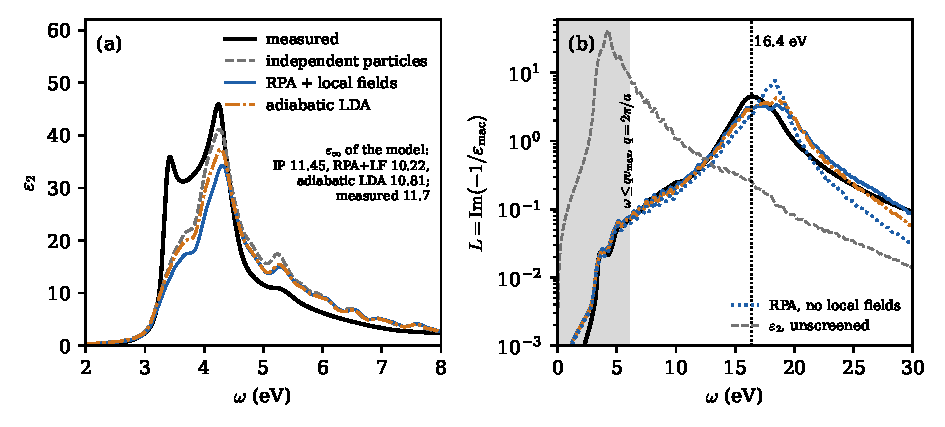
\includegraphics[width=\linewidth]{figures/ch04/fig4_7.pdf}
  \caption{Three many-body approximations to the dielectric function of crystalline silicon at $\vect{q} \to 0$, in a model calculation. Band energies and Bloch states come from the local empirical pseudopotential of Cohen and Bergstresser~\cite{cohen1966band}, fitted to measured transition energies (no scissor shift). The sums run over a shifted $20^3$ grid of $\vect{k}$ points over the full zone, with 4 valence and 26 conduction bands, a local-field matrix of the 59 shortest reciprocal vectors, and a Lorentzian broadening of \SI{0.10}{eV}. The exchange--correlation kernel is the adiabatic local-density one, evaluated on the model's valence density with the Perdew--Zunger correlation energy~\cite{perdew1981self}. Black: measured at \SI{300}{K}~\cite{franta2017temperature}; panel (a) lists the static limits of the three approximations against the measured $\varepsilon_\infty = 11.7$ (\cref{sec:4.4}). (a) Absorptive part $\varepsilon_2$: independent particles (dashed gray), which is also the random-phase approximation without local fields; the random-phase approximation with local fields (solid blue); adiabatic LDA (dash-dotted orange). The strength of the measured lower peak at \SI{3.42}{eV} comes from the electron--hole attraction (\cref{sec:4.9}), and all three underestimate it. (b) Loss function on a logarithmic scale: the random-phase approximation without local fields (dotted blue), with local fields (solid blue), and adiabatic LDA (dash-dotted orange). Dashed gray: the unscreened $\varepsilon_2$ of independent particles, which a rate without screening would use in place of $L$. The model's loss peak lies about \SI{2}{eV} above the measured \SI{16.4}{eV} (dotted line), because its high conduction bands are not fitted. Shaded: energies up to $qv_{\mathrm{max}} = \SI{6.05}{eV}$ at a momentum transfer of one reciprocal-lattice unit, $q = 2\pi/a$, the range that dark matter of any mass can reach there.}
  \label{fig:4-si-approx}
\end{figure}

Panel (b) shows the loss function that sets the dark-matter rate. Up to about \SI{6}{eV} the loss function lies two to three orders of magnitude below the unscreened $\varepsilon_2$; this is the factor $1/|\varepsilon|^2$ that the head of the dielectric matrix already contains. On this scale the local fields are a correction of tens of percent. Between 3 and \SI{12}{eV} they raise $L$ by 10 to 35 percent, because they lower $|\varepsilon|$, and they cut the height of the plasmon peak from 7.6 to 3.4. A dark-matter rate integrates the loss function over $\vect{q}$ and over $\omega$ up to $qv_{\mathrm{max}}$, and for silicon and germanium the difference between rates computed with and without local fields is small~\cite{knapen2021dark}. Local fields matter more at momentum transfers of a few reciprocal vectors, where the off-diagonal elements of $R^0$ are as large as the diagonal ones, and at energies where semicore shells, localized near the nuclei, contribute.

Local fields have a second reading, which \cref{sec:4.9} uses. In the space of electron--hole pairs, the microscopic Hartree potential $\bar v$ is the bare Coulomb interaction between a pair and another pair at the same total momentum, with the long-range term at $\vect{G} = 0$ removed. This is the exchange kernel $K^{\mathrm{x}}$ of the Bethe--Salpeter equation. The random-phase approximation with local fields is that equation with the electron--hole attraction switched off, and it cannot bind an exciton.

\subsection{Time-dependent density-functional theory}

The bubble \cref{eq:4.6-R0} is built from Kohn--Sham states, and until now that was a convenience: the states of some independent-particle model were needed, and these were at hand. Time-dependent density-functional theory makes the choice exact. Runge and Gross proved that the time-dependent density of an interacting system, evolving from its ground state, determines the time-dependent external potential up to a function of time alone~\cite{runge1984density}. It follows, as in the static theory, that a system of independent electrons in a suitable time-dependent Kohn--Sham potential has the same density at all times. That potential is the external one plus the Hartree potential plus an exchange--correlation potential $v_{\mathrm{xc}}(\vect{r},t)$, which now depends on the density at all earlier times.

Linear response follows in three lines. A weak external potential energy $\phi_{\mathrm{ext}}$ changes the Kohn--Sham potential by
\begin{equation*}
  \delta V_{\mathrm{KS}}(\vect{r},t) = \phi_{\mathrm{ext}}(\vect{r},t) + \int\dd^3r'\,v_{\mathrm{C}}(\vect{r} - \vect{r}')\,\delta\nd(\vect{r}',t)
  + \int\dd^3r'\int\dd t'\,f_{\mathrm{xc}}(\vect{r},\vect{r}',t - t')\,\delta\nd(\vect{r}',t') ,
\end{equation*}
where the exchange--correlation kernel
\begin{equation}
  f_{\mathrm{xc}}(\vect{r},\vect{r}',t - t') = \frac{\delta v_{\mathrm{xc}}(\vect{r},t)}{\delta\nd(\vect{r}',t')}\bigg|_{\nd_{\mathrm{gs}}} ,
  \label{eq:4.6-fxc}
\end{equation}
is the functional derivative taken at the ground-state density $\nd_{\mathrm{gs}}$. Since the Kohn--Sham electrons are independent, their density responds to their own potential through the bubble: $\delta\nd = R^0\,\delta V_{\mathrm{KS}}$, with $R^0$ of \cref{eq:4.6-R0}. And $\delta\nd$ is, by construction, the density change of the interacting system, $\delta\nd = R\,\phi_{\mathrm{ext}}$. In reciprocal space, with $f_{\mathrm{Hxc}} = v_{\mathrm{C}} + f_{\mathrm{xc}}$ the matrix $(f_{\mathrm{Hxc}})_{\vect{G}\vect{G}'} = v_{\mathrm{C}}(|\vect{q}+\vect{G}|)\delta_{\vect{G}\vect{G}'} + (f_{\mathrm{xc}})_{\vect{G}\vect{G}'}(\vect{q},\omega)$, the two statements combine to $R\phi_{\mathrm{ext}} = R^0(\phi_{\mathrm{ext}} + f_{\mathrm{Hxc}}R\phi_{\mathrm{ext}})$ for every $\phi_{\mathrm{ext}}$.
\begin{keyresult}[Dyson equation of time-dependent density-functional theory]
\begin{equation}
  R = R^0 + R^0 f_{\mathrm{Hxc}} R, \qquad \tilde R = R^0 + R^0 f_{\mathrm{xc}}\tilde R ,
  \label{eq:4.6-tddft}
\end{equation}
as matrices in the reciprocal-lattice vectors at fixed $(\vect{q},\omega)$. With the exact kernel, $R$ is the exact density response, although $R^0$ is built from Kohn--Sham states. The random-phase approximation is $f_{\mathrm{xc}} = 0$.
\end{keyresult}
The proper response follows from the first form by splitting off the Coulomb kernel, since $R = \tilde R + \tilde Rv_{\mathrm{C}}R$ (\cref{eq:4.4-dyson}) has the solution $\tilde R = (1 - R^0f_{\mathrm{xc}})^{-1}R^0$. This is \cref{eq:E.6-dyson}, and Petersilka, Gossmann and Gross used it to compute excitation energies as the poles of $R$~\cite{petersilka1996excitation}. For the macroscopic function, the kernel of \cref{eq:4.6-rpaLF} becomes $\bar v + f_{\mathrm{xc}}$, with the long-range Coulomb term still removed.

The exact kernel, however, is unknown. The Kohn--Sham gap is smaller than the true one (\cref{sec:3.4}), and the poles of $R^0$ lie at the wrong energies; the kernel must move them. It must also bind the electron and the hole into excitons, which takes an attraction of long range. Both are hard to get from a function of the density at one point.

The most widely used kernel is the \emph{adiabatic local-density approximation} (ALDA). It takes the exchange--correlation potential of \cref{eq:3.4-LDA} at the instantaneous local density, so that the kernel is local in space and instantaneous in time~\cite{gross1985local},
\begin{equation}
  f_{\mathrm{xc}}^{\mathrm{ALDA}}(\vect{r},\vect{r}',t - t') = \delta(\vect{r} - \vect{r}')\,\delta(t - t')\,\frac{\dd^2\bigl[\nd\,\varepsilon_{\mathrm{xc}}(\nd)\bigr]}{\dd\nd^2}\bigg|_{\nd_{\mathrm{gs}}(\vect{r})} .
  \label{eq:4.6-alda}
\end{equation}
It is negative, since exchange and correlation make the potential more attractive where the density grows. In reciprocal space it is a function of $\vect{G} - \vect{G}'$ alone and does not depend on $\vect{q}$ or $\omega$.

These properties fix what the kernel misses. Being instantaneous, it has no frequency dependence and cannot open the gap: the absorption edge stays at the Kohn--Sham gap, and a scissor or quasiparticle energies are still needed. Being local, its matrix is finite as $\vect{q} \to 0$. In the optical limit the head element enters $\tilde R_{\vect{0}\vect{0}}$ multiplied by $R^0_{\vect{0}\vect{0}} = O(q^2)$ and drops out, and the wings drop out with one power of $q$. The kernel acts only through the body of the matrix, at $\vect{G}, \vect{G}' \neq 0$, alongside $\bar v$, which it partly cancels. An exciton, however, needs the attraction between an electron and a hole at large separation, which in an insulator behaves as $-\alpha_{\mathrm{xc}}/|\vect{q}+\vect{G}|^2$ in reciprocal space~\cite{reining2002excitonic}; a local kernel has no such term. In \cref{fig:4-si-approx} the adiabatic LDA spectrum lies between the two random-phase ones and close to the one with local fields, with the upper peak at a height of 37, and its static constant lies between theirs (\cref{we:4-siepsinf}). Its lower peak is as weak as theirs. This is the general finding for semiconductors: for absorption the adiabatic LDA is little better than the random-phase approximation with local fields, and for energy-loss spectra it does well because the random-phase approximation already does~\cite{onida2002electronic,botti2007time}.

\subsection{Local-field factor of the electron gas}

In the homogeneous gas every matrix is diagonal, and \cref{eq:4.6-tddft} gives $\tilde R = R^0/(1 - f_{\mathrm{xc}}R^0)$ with the Lindhard function $R^0$ of \cref{eq:4.5-lindhard}. The many-body literature on the gas writes the same proper response with a static \emph{local-field factor} $G_{\mathrm{LF}}(q)$. It is defined by
\begin{equation*}
  \varepsilon(q,\omega) = 1 - \frac{v_{\mathrm{C}}(q)\,R^0(q,\omega)}{1 + v_{\mathrm{C}}(q)\,G_{\mathrm{LF}}(q)\,R^0(q,\omega)} .
\end{equation*}
An electron feels the Hartree potential of the induced density reduced by the factor $1 - G_{\mathrm{LF}}$, because the exchange--correlation hole keeps the other electrons away from it. The name is the gas analog of the local fields of a crystal: in both cases the field an electron actually feels differs from the average one. Comparing with $\varepsilon = 1 - v_{\mathrm{C}}R^0/(1 - f_{\mathrm{xc}}R^0)$,
\begin{equation}
  f_{\mathrm{xc}}(q) = -v_{\mathrm{C}}(q)\,G_{\mathrm{LF}}(q) = -\frac{e^2}{q^2}\,G_{\mathrm{LF}}(q) .
  \label{eq:4.6-GLF}
\end{equation}
A static local-field factor is thus a static kernel, and every model of $G_{\mathrm{LF}}$ in the literature on the gas~\cite[Chap.~5]{giuliani2005quantum} is a kernel of time-dependent density-functional theory for it.

The long-wavelength limit is fixed by thermodynamics. A static potential of long wavelength shifts the local chemical potential, as in the Thomas--Fermi argument of \cref{sec:4.4}, and the proper response is $\tilde R(q\to0,0) = -\partial\nd_e/\partial\mu_{\mathrm{ch}}$, with $\mu_{\mathrm{ch}}$ the chemical potential without the Hartree term. With $R^0(q\to0,0) = -2\mathcal{N}_{\mathrm{F}}$, the inverse of $\tilde R = R^0/(1 - f_{\mathrm{xc}}R^0)$ is
\begin{equation}
  \frac{\partial\mu_{\mathrm{ch}}}{\partial\nd_e} = \frac{1}{2\mathcal{N}_{\mathrm{F}}} + f_{\mathrm{xc}}(q\to0) ,
  \label{eq:4.6-compress}
\end{equation}
which is the compressibility sum rule: the kernel at long wavelength is the second derivative of the exchange--correlation energy density, $\dd^2(\nd\varepsilon_{\mathrm{xc}})/\dd\nd^2$. The adiabatic LDA satisfies it by construction. For exchange alone, $v_{\mathrm{x}} = \tfrac43\varepsilon_{\mathrm{x}} \propto \nd^{1/3}$ with $\varepsilon_{\mathrm{x}} = -3e^2k_{\mathrm{F}}/16\pi^2$, so $f_{\mathrm{x}} = \dd v_{\mathrm{x}}/\dd\nd = v_{\mathrm{x}}/3\nd$, and with $\nd = k_{\mathrm{F}}^3/3\pi^2$,
\begin{equation*}
  f_{\mathrm{x}} = -\frac{e^2}{4k_{\mathrm{F}}^2}, \qquad G_{\mathrm{LF}}(q) = \frac{q^2}{4k_{\mathrm{F}}^2}\quad (q \ll k_{\mathrm{F}}) .
\end{equation*}
Correlation adds to this. At $r_s = 2$, the Perdew--Zunger correlation energy~\cite{perdew1981self} raises the coefficient from $\tfrac14$ to 0.267, and \cref{eq:4.6-compress} with $k_{\mathrm{TF}}^2/k_{\mathrm{F}}^2 = 1.33$ (\cref{sec:4.5}) says that the gas is 1.55 times more compressible than free electrons of the same density. An electron surrounded by its exchange--correlation hole repels the others less, the gas yields more easily to a slow potential, and it screens more strongly than the random-phase approximation says.

The adiabatic LDA fails at short wavelengths, where dark matter scatters. Its $G_{\mathrm{LF}} = 0.267\,q^2/k_{\mathrm{F}}^2$ grows without bound, while the factor of the real gas follows the $q^2$ law only for $q \ll k_{\mathrm{F}}$; beyond $q \sim k_{\mathrm{F}}$ it stops growing and stays of order one~\cite[Chap.~5]{giuliani2005quantum}. At the typical momentum transfer $q_0 = \SI{3.73}{keV}$, which is $1.04\,k_{\mathrm{F}}$ at the silicon valence density, the local kernel is at the edge of its range of validity. There its factor is 0.29, and it raises the static Lindhard value $\varepsilon(q_0,0) = 2.10$ of \cref{sec:4.5} to 2.62. The correction to the screening at $q_0$ is thus of order a quarter. Its sign is reliable, its size at $q \sim k_{\mathrm{F}}$ only to the extent that the local kernel is.

\subsection{Many-body spread as an error measure}

Independent particles, the random-phase approximation with the head alone, the same with local fields, and an exchange--correlation kernel on top form a hierarchy, which the Bethe--Salpeter equation of \cref{sec:4.9} completes. The hierarchy is not an expansion in a small number: each level adds a physical effect whose size depends on the material, the energy and the momentum, so no level bounds the error of the one below. The hierarchy does measure how much a quantity depends on the many-body treatment. In silicon the static constant changes by about a tenth across the approximations of \cref{fig:4-si-approx} (\cref{we:4-siepsinf}), and the screening factor $1/\varepsilon_\infty^2$ at small $q$ by about a quarter. Near the gap, where excitons move weight, the spread is larger, and only the Bethe--Salpeter equation captures the shape of the spectrum there. Well above the gap, at the energies that hold most of the f-sum, the approximations agree to within the accuracy of the bands. This many-body spread, computed with the same bands, $\vect{k}$ grid and cutoffs in every approximation, is the many-body part of the theory uncertainty of a loss function. For heavier dark matter, whose rate is dominated by energies of several eV, it is small. For light dark matter, which deposits at most $\tfrac12\mchi v_{\mathrm{max}}^2$ (\cref{eq:1.3-omegamax}) and so samples the first eV above the gap, it is the leading part.

\begin{workedexample}{The local-field reduction of the dielectric constant of silicon}\label{we:4-siepsinf}
The calculation of \cref{fig:4-si-approx} yields the static limit of each approximation at $\vect{q} \to 0$ from the same states, from \cref{eq:4.6-static} for independent particles and from \cref{eq:4.6-rpaLF,eq:4.6-tddft} at $\omega = 0$ for the others. Independent particles, and equally the random-phase approximation without local fields, give $\varepsilon_\infty = 11.45$, within 2 percent of the measured 11.7. The small difference is a property of the model, whose form factors were fitted to measured transition energies. With the local fields of the 59 shortest reciprocal vectors, $\varepsilon_\infty = 10.22$, unchanged to three digits with 113 vectors; the local fields lower the dielectric constant by 11 percent. The adiabatic LDA kernel raises it again to 10.81, 6 percent above the random-phase value with local fields, so that it cancels about half of the local-field reduction. All three are converged in the $\vect{k}$ grid to better than 0.1 percent.

The PBE value 13.04 of \cref{sec:3.4} is a static linear-response calculation with Kohn--Sham bands, local fields and the adiabatic PBE kernel: it is the third of our approximations, with Kohn--Sham energies in place of fitted ones. It lies above the measured value by 11 percent, and the reason is \cref{eq:4.6-static}. The PBE gap is about half the measured one, and the static sum weights small transition energies by their inverse cube. The same representative PBE setting as \cref{app:E.1}, at the measured lattice constant on a $20^3$ grid, gives the other two approximations as well: 13.61 for independent particles and 12.20 with local fields, against 13.04 with the PBE kernel. The first-principles values follow the trend of the model values 11.45, 10.22 and 10.81: the local fields lower $\varepsilon_\infty$ by 10 percent, and the kernel restores part of it. Independent particles with fitted energies happen to land close to experiment, but the adiabatic kernel with fitted energies does not: at 10.81 it is 8 percent below 11.7. The adiabatic kernel lacks the electron--hole attraction, which lowers the energies of the transitions near the gap and so raises $\varepsilon_\infty$ (\cref{sec:4.9}).

For a dark-matter rate at momentum transfers small enough that $L \simeq \varepsilon_2/\varepsilon_\infty^2$, the local-field reduction of $\varepsilon_\infty$ alone changes the screening factor by $(11.45/10.22)^2 \simeq 1.25$. The kernel undoes part of it, and the electron--hole attraction more than makes up the rest.
\end{workedexample}

\section{Green's functions}\label{sec:4.7}

The Bethe--Salpeter equation, which completes the hierarchy of \cref{sec:4.6}, needs quasiparticle energies and a screened interaction, and both are properties of one added electron. Put one extra electron into the conduction band of silicon. The other electrons move away from it and screen its charge, the lattice relaxes around it, and if it lies high enough in the band it can lose energy by creating an electron--hole pair or by emitting a phonon. The electron propagates dressed by its surroundings, with an energy that differs from its Kohn--Sham band energy and, in general, with a finite lifetime. The density response $R_{ee}$ of \cref{sec:4.1} does not follow this dressed electron, since the density operator moves an electron from one state to another and never changes their number. The function that does is the single-particle Green's function $\GF$: the amplitude that an electron added to the target at one time is still found in the same state at a later time. Its poles are the energies of the dressed electrons, the quasiparticles of the target, and the distance of each pole below the real axis is a decay rate. The treatment follows Refs.~\cite{bruus2004many}, \cite[Chaps.~3 and 7]{fetter1971quantum} and \cite[Chaps.~2 and 3]{mahan2000many}.

\subsection{The one-electron Green's function}

The Green's function changes the number of electrons, so we work in the grand-canonical state \cref{eq:2.5-grand}, with $\op{N}_e$ the electron number operator of \cref{sec:2.3}. Every Heisenberg operator in this section evolves with $H_\mu = H - \mu_{\mathrm{ch}}\op{N}_e$, so that $c(t) = \ee^{\ii H_\mu t}c\,\ee^{-\ii H_\mu t}$, and $E_i$ denotes an eigenvalue of $H_\mu$. Energies are then measured from the chemical potential: adding an electron to the $N$-electron state $|i\rangle$ to reach the $(N+1)$-electron state $|f\rangle$ costs $E_f - E_i$ in eigenvalues of $H_\mu$, which is the change of the total energy minus $\mu_{\mathrm{ch}}$. Let $c^\dagger_{\vect{k}}$ create an electron in a single-particle state labeled $\vect{k}$, with the spin and, in a crystal, the band index included in the label. The retarded Green's function is
\begin{equation}
  \GF^{\mathrm{R}}(\vect{k},t) = -\ii\,\Theta(t)\,\bigl\langle\{c_{\vect{k}}(t),\,c^\dagger_{\vect{k}}(0)\}\bigr\rangle ,
  \label{eq:4.7-GR}
\end{equation}
with the anticommutator $\{A, B\} = AB + BA$ and the average in the grand-canonical state. It has the form of the response function \cref{eq:4.1-kubo}, with an anticommutator in place of the commutator. The term $\langle c_{\vect{k}}(t)c^\dagger_{\vect{k}}\rangle$ is the overlap of the state with an electron added in $\vect{k}$ at time $0$ with the same state at time $t$: the amplitude that the added electron is still there. The term $\langle c^\dagger_{\vect{k}}c_{\vect{k}}(t)\rangle$ is the same amplitude for a hole, an electron removed from $\vect{k}$. The anticommutator makes $\GF^{\mathrm{R}}(\vect{k},0^+) = -\ii$ whatever the state, since $\{c_{\vect{k}}, c^\dagger_{\vect{k}}\} = 1$ (\cref{eq:2.3-anticomm}).

For independent electrons the amplitude is a pure phase. With $H_\mu = \sum_{\vect{k}}\xi_{\vect{k}}\,c^\dagger_{\vect{k}}c_{\vect{k}}$, where $\xi_{\vect{k}}$ is the energy of the orbital $\vect{k}$ of \cref{sec:2.3} measured from $\mu_{\mathrm{ch}}$, the Heisenberg operator is $c_{\vect{k}}(t) = c_{\vect{k}}\,\ee^{-\ii\xi_{\vect{k}}t}$ (\cref{sec:2.3}). The anticommutator in \cref{eq:4.7-GR} is then the number $\ee^{-\ii\xi_{\vect{k}}t}$, and with the transform of \cref{app:A.3} and $\omega \to \omega + \ii0^+$, as for every retarded function (\cref{sec:4.1}),
\begin{equation}
  \GF^{\mathrm{R}}_0(\vect{k},t) = -\ii\,\Theta(t)\,\ee^{-\ii\xi_{\vect{k}}t}, \qquad
  \GF^{\mathrm{R}}_0(\vect{k},\omega) = \frac{1}{\omega - \xi_{\vect{k}} + \ii0^+} .
  \label{eq:4.7-G0}
\end{equation}
The subscript $0$ marks the function without interactions. It has one pole, at the energy of the orbital, and it is independent of temperature and of which orbitals are occupied.

In an interacting target the same steps as in \cref{sec:4.1} lead to the eigenstates. Inserting a complete set of states between the operators, $\langle c_{\vect{k}}(t)c^\dagger_{\vect{k}}\rangle = \sum_{i,f}p_i\,|\langle f|c^\dagger_{\vect{k}}|i\rangle|^2\,\ee^{-\ii(E_f - E_i)t}$ and $\langle c^\dagger_{\vect{k}}c_{\vect{k}}(t)\rangle = \sum_{i,f}p_i\,|\langle f|c_{\vect{k}}|i\rangle|^2\,\ee^{+\ii(E_f - E_i)t}$, and the time integrals are those of \cref{eq:4.1-lehmann}. Since the two terms are added, not subtracted, both enter with a plus sign:
\begin{keyresult}[Lehmann representation of the Green's function]
\begin{equation}
  \begin{aligned}
  \GF^{\mathrm{R}}(\vect{k},\omega) &= \sum_{i,f}p_i\left[\frac{|\langle f|c^\dagger_{\vect{k}}|i\rangle|^2}{\omega - (E_f - E_i) + \ii0^+} + \frac{|\langle f|c_{\vect{k}}|i\rangle|^2}{\omega + (E_f - E_i) + \ii0^+}\right] \\
  &= \int\dd\omega'\,\frac{\SpecA(\vect{k},\omega')}{\omega - \omega' + \ii0^+} ,
  \end{aligned}
  \label{eq:4.7-lehmann}
\end{equation}
with the spectral function
\begin{equation}
  \begin{aligned}
  \SpecA(\vect{k},\omega) &= -\frac{1}{\pi}\Imag\GF^{\mathrm{R}}(\vect{k},\omega) \\
  &= \sum_{i,f}p_i\Bigl[|\langle f|c^\dagger_{\vect{k}}|i\rangle|^2\,\delta\bigl(\omega - (E_f - E_i)\bigr) + |\langle f|c_{\vect{k}}|i\rangle|^2\,\delta\bigl(\omega + (E_f - E_i)\bigr)\Bigr] .
  \end{aligned}
  \label{eq:4.7-A}
\end{equation}
The poles are at the energies needed to add an electron in $\vect{k}$, and at minus the energies released by removing one, each weighted by the probability that the added electron or hole is found in an exact eigenstate.
\end{keyresult}
This is the representation of Lehmann~\cite{lehmann1954uber}, and it shows that $\SpecA$ is positive, normalized, and tied to the occupations. It is positive since every weight in \cref{eq:4.7-A} is. Its integral over $\omega$ is $\sum_ip_i\langle i|c_{\vect{k}}c^\dagger_{\vect{k}} + c^\dagger_{\vect{k}}c_{\vect{k}}|i\rangle = 1$, which makes $\SpecA(\vect{k},\omega)$ a probability density in energy: the probability that an electron or hole put into $\vect{k}$ has the energy $\omega$. And the removal part alone counts the electrons already in $\vect{k}$. To see this, relabel $i \leftrightarrow f$ in the removal term; it becomes $\sum_{i,f}p_f\,|\langle f|c^\dagger_{\vect{k}}|i\rangle|^2\,\delta(\omega - (E_f - E_i))$, and on the energy shell $p_f = p_i\,\ee^{-\beta\omega}$, the detailed-balance step of \cref{eq:2.5-db}. The removal part is thus $\ee^{-\beta\omega}$ times the addition part, the two add up to $\SpecA$, and the removal part is $\SpecA\,\ee^{-\beta\omega}/(1 + \ee^{-\beta\omega}) = \SpecA\,n_{\mathrm{F}}(\omega)$. Its integral is $\langle c^\dagger_{\vect{k}}c_{\vect{k}}\rangle$:
\begin{equation}
  \langle c^\dagger_{\vect{k}}c_{\vect{k}}\rangle = \int\dd\omega\,\SpecA(\vect{k},\omega)\,n_{\mathrm{F}}(\omega) .
  \label{eq:4.7-occ}
\end{equation}
For independent electrons $\SpecA_0(\vect{k},\omega) = \delta(\omega - \xi_{\vect{k}})$ and \cref{eq:4.7-occ} is the Fermi function of \cref{eq:2.5-nF}. With interactions the occupation of a plane-wave state is no longer $n_{\mathrm{F}}(\xi_{\vect{k}})$, even at $T = 0$, because $\SpecA$ has weight at energies other than $\xi_{\vect{k}}$. Note that we normalize $\SpecA$ to one. Many texts, Refs.~\cite{bruus2004many,mahan2000many} among them, write $-2\Imag\GF^{\mathrm{R}}$ for the spectral function, which integrates to $2\pi$.

The spectral function is close to a measured quantity. In photoemission a photon removes an electron from the crystal, and the rate at a given energy and momentum of the outgoing electron is, in the simplest approximation, proportional to the removal part $\SpecA\,n_{\mathrm{F}}$; inverse photoemission measures the addition part. The analytic structure is that of \cref{sec:4.1}. By \cref{eq:4.7-lehmann}, $\GF^{\mathrm{R}}(\vect{k},z) = \int\dd\omega'\,\SpecA(\vect{k},\omega')/(z - \omega')$ is analytic in the upper half plane, and the advanced function $\GF^{\mathrm{A}}(\vect{k},\omega) = \GF^{\mathrm{R}}(\vect{k},\omega)^*$, nonzero only for $t < 0$, is its boundary value from below.

\subsection{The time-ordered function}

At $T = 0$ the perturbation theory of \cref{sec:4.8} produces a third function. The Dyson series \cref{eq:2.4-dyson} is a time-ordered exponential, and when it is used to expand a ground-state amplitude the operators come out in time order. The time-ordered Green's function is
\begin{equation}
  \GF(\vect{k},t) = -\ii\,\langle0|\mathrm{T}\,c_{\vect{k}}(t)\,c^\dagger_{\vect{k}}(0)|0\rangle
  = -\ii\,\Theta(t)\,\langle0|c_{\vect{k}}(t)\,c^\dagger_{\vect{k}}|0\rangle + \ii\,\Theta(-t)\,\langle0|c^\dagger_{\vect{k}}\,c_{\vect{k}}(t)|0\rangle ,
  \label{eq:4.7-GT}
\end{equation}
where $|0\rangle$ is the ground state of $H_\mu$ and the time-ordering symbol $\mathrm{T}$ puts the operator with the later time on the left, with a minus sign when two fermion operators are exchanged. For $t > 0$ it propagates an added electron forward in time, and for $t < 0$ a hole. The integral over $t > 0$ is that of the retarded function. The integral over $t < 0$ needs a factor $\ee^{+0^+t}$ to converge, $\ii\int_{-\infty}^0\dd t\,\ee^{\ii(\omega + E_f - E_0)t + 0^+t} = 1/(\omega + E_f - E_0 - \ii0^+)$, so
\begin{equation}
  \GF(\vect{k},\omega) = \sum_f\left[\frac{|\langle f|c^\dagger_{\vect{k}}|0\rangle|^2}{\omega - (E_f - E_0) + \ii0^+} + \frac{|\langle f|c_{\vect{k}}|0\rangle|^2}{\omega + (E_f - E_0) - \ii0^+}\right] .
  \label{eq:4.7-GTlehmann}
\end{equation}
The removal poles now lie above the real axis. At $T = 0$ every $E_f - E_0 \ge 0$, because $|0\rangle$ is the ground state of $H_\mu$ in all particle-number sectors. The addition poles therefore lie at $\omega > 0$ and the removal poles at $\omega < 0$. As a result, the time-ordered function equals $\GF^{\mathrm{R}}$ for $\omega > 0$ and $\GF^{\mathrm{A}}$ for $\omega < 0$, and both carry the same spectral function. In this section a $\GF$ without superscript and with a real time or frequency is the time-ordered function. With an imaginary argument it is the Matsubara function introduced below, and with a complex argument $z$ it is the function $\int\dd\omega'\,\SpecA(\vect{k},\omega')/(z - \omega')$, which unites them all.

\subsection{Self-energy and the Dyson equation}

How does an interaction change $\GF^{\mathrm{R}}$? Split $H_\mu = \sum_{\vect{k}}\xi_{\vect{k}}\,c^\dagger_{\vect{k}}c_{\vect{k}} + H_{\mathrm{int}}$, where $H_{\mathrm{int}}$ holds the Coulomb interaction between the electrons, their coupling to phonons, or any other term that is not a one-body energy. The Heisenberg operator obeys $\ii\,\partial_tc_{\vect{k}}(t) = [c_{\vect{k}}, H_\mu](t) = \xi_{\vect{k}}c_{\vect{k}}(t) + [c_{\vect{k}}, H_{\mathrm{int}}](t)$, by \cref{eq:2.3-bilinear}. Differentiating \cref{eq:4.7-GR}, the derivative of the step function gives $\delta(t)\langle\{c_{\vect{k}}, c^\dagger_{\vect{k}}\}\rangle = \delta(t)$, and
\begin{equation*}
  \ii\,\partial_t\GF^{\mathrm{R}}(\vect{k},t) = \delta(t) + \xi_{\vect{k}}\,\GF^{\mathrm{R}}(\vect{k},t) + \mathsf{F}^{\mathrm{R}}(\vect{k},t), \qquad
  \mathsf{F}^{\mathrm{R}}(\vect{k},t) = -\ii\,\Theta(t)\,\bigl\langle\{[c_{\vect{k}}, H_{\mathrm{int}}](t),\,c^\dagger_{\vect{k}}\}\bigr\rangle .
\end{equation*}
The function $\mathsf{F}^{\mathrm{R}}$ is a retarded correlation of the same kind, built from the operator $[c_{\vect{k}}, H_{\mathrm{int}}]$, which removes an electron from $\vect{k}$ and scatters the others. With $\ee^{\ii\omega t}$, the derivative $\ii\,\partial_t$ becomes $\omega$, and $(\omega - \xi_{\vect{k}})\,\GF^{\mathrm{R}} = 1 + \mathsf{F}^{\mathrm{R}}$. We define the self-energy $\Sigma^{\mathrm{R}}(\vect{k},\omega)$ as the ratio $\mathsf{F}^{\mathrm{R}}/\GF^{\mathrm{R}}$. This is possible because $\GF^{\mathrm{R}}(\vect{k},z)$ has no zeros in the upper half plane: there $\Imag\GF^{\mathrm{R}}(\vect{k},z) = -\Imag z\int\dd\omega'\,\SpecA(\vect{k},\omega')/|z - \omega'|^2 < 0$ by the positivity of $\SpecA$. Multiplying by $\GF^{\mathrm{R}}_0$ of \cref{eq:4.7-G0} gives the Dyson equation.
\begin{keyresult}[Dyson equation]
\begin{equation}
  \begin{gathered}
  \GF^{\mathrm{R}}(\vect{k},\omega) = \GF^{\mathrm{R}}_0(\vect{k},\omega) + \GF^{\mathrm{R}}_0(\vect{k},\omega)\,\Sigma^{\mathrm{R}}(\vect{k},\omega)\,\GF^{\mathrm{R}}(\vect{k},\omega), \\
  \GF^{\mathrm{R}}(\vect{k},\omega) = \frac{1}{\omega - \xi_{\vect{k}} - \Sigma^{\mathrm{R}}(\vect{k},\omega)} .
  \end{gathered}
  \label{eq:4.7-dyson}
\end{equation}
All the effects of the interaction on the propagation of one electron are in the self-energy $\Sigma^{\mathrm{R}}$, a complex function of energy.
\end{keyresult}
In a crystal, with $\vect{k}$ the crystal momentum and $n$ the band, the same steps make $\GF^{\mathrm{R}}$ and $\Sigma^{\mathrm{R}}$ matrices in the band indices, and \cref{eq:4.7-dyson} a matrix equation of the type \cref{eq:C.7-dyson}. In a translation-invariant target they are diagonal in $\vect{k}$, as we assume here.

So far \cref{eq:4.7-dyson} is a definition. Its content appears when it is iterated: $\GF^{\mathrm{R}} = \GF^{\mathrm{R}}_0 + \GF^{\mathrm{R}}_0\Sigma^{\mathrm{R}}\GF^{\mathrm{R}}_0 + \GF^{\mathrm{R}}_0\Sigma^{\mathrm{R}}\GF^{\mathrm{R}}_0\Sigma^{\mathrm{R}}\GF^{\mathrm{R}}_0 + \cdots$. The electron propagates freely, is scattered out of $\vect{k}$ and back by the interaction, propagates freely again, and so on, and $\Sigma^{\mathrm{R}}$ is the amplitude of one such excursion. \Cref{sec:4.8} computes $\Sigma$ with diagrams and shows that it is the sum of the excursions that cannot be cut into two by removing a single free propagator. A self-energy known only to low order then yields a Green's function to all orders, and no finite order of the series has the shifted, broadened pole that the closed form has (\cref{app:C.7}). This is what the width did for the intermediate state of \cref{sec:2.4}, where summing the repeated emission and reabsorption turned $\ii0^+$ into $\ii\varGamma_{\mathrm{w}}/2$ in \cref{eq:2.4-width}.

The sign of the width is fixed before any calculation. On the real axis, $\Sigma^{\mathrm{R}} = \omega - \xi_{\vect{k}} - 1/\GF^{\mathrm{R}}$ has the imaginary part $\Imag\GF^{\mathrm{R}}/|\GF^{\mathrm{R}}|^2$, so
\begin{equation}
  \Imag\Sigma^{\mathrm{R}}(\vect{k},\omega) = -\frac{\pi\,\SpecA(\vect{k},\omega)}{\bigl|\GF^{\mathrm{R}}(\vect{k},\omega)\bigr|^2} \le 0 .
  \label{eq:4.7-ImSigma}
\end{equation}
The large-frequency limit is fixed as well. At large $|\omega|$, the expansion $1/(\omega - \omega') = \omega^{-1} + \omega'\omega^{-2} + \cdots$ in \cref{eq:4.7-lehmann} gives $\GF^{\mathrm{R}} = \omega^{-1} + m_1\omega^{-2} + O(\omega^{-3})$, with $m_1 = \int\dd\omega\,\omega\,\SpecA = \langle\{[c_{\vect{k}}, H_\mu], c^\dagger_{\vect{k}}\}\rangle$ by the same steps as \cref{eq:4.1-tail}. Then $1/\GF^{\mathrm{R}} = \omega - m_1 + O(\omega^{-1})$, and $\Sigma^{\mathrm{R}}(\vect{k},\omega) \to m_1 - \xi_{\vect{k}} = \langle\{[c_{\vect{k}}, H_{\mathrm{int}}], c^\dagger_{\vect{k}}\}\rangle$. The self-energy tends to a static potential, linear in $H_{\mathrm{int}}$ and evaluated in the exact state. For the Coulomb interaction it is the mean-field (Hartree and exchange) potential, built with the exact occupations. Everything that depends on frequency, the retardation of the screening and the decay into other excitations, is in $\Sigma^{\mathrm{R}} - \Sigma^{\mathrm{R}}(\vect{k},\infty)$, which is analytic in the upper half plane and falls off at large $|\omega|$, and as a result obeys the Kramers--Kronig relations of \cref{app:C.5}.

\subsection{Quasiparticles}

Suppose the self-energy is small and varies slowly with $\omega$. The Green's function \cref{eq:4.7-dyson} is then large where its real denominator vanishes, at the quasiparticle energy $E_{\mathrm{qp}}(\vect{k})$ defined by
\begin{equation*}
  E_{\mathrm{qp}}(\vect{k}) - \xi_{\vect{k}} - \Real\Sigma^{\mathrm{R}}\bigl(\vect{k},E_{\mathrm{qp}}(\vect{k})\bigr) = 0 .
\end{equation*}
Near this energy we expand the real part to first order, $\omega - \xi_{\vect{k}} - \Real\Sigma^{\mathrm{R}} \simeq (\omega - E_{\mathrm{qp}})/z_{\mathrm{qp}}$, and keep the imaginary part at its value at $E_{\mathrm{qp}}$.
\begin{keyresult}[Quasiparticle]
\begin{equation}
  \begin{gathered}
  \GF^{\mathrm{R}}(\vect{k},\omega) \simeq \frac{z_{\mathrm{qp}}(\vect{k})}{\omega - E_{\mathrm{qp}}(\vect{k}) + \ii\varGamma_{\mathrm{qp}}(\vect{k})/2}, \\
  z_{\mathrm{qp}} = \Bigl[1 - \partial_\omega\Real\Sigma^{\mathrm{R}}(\vect{k},\omega)\big|_{E_{\mathrm{qp}}}\Bigr]^{-1}, \qquad
  \varGamma_{\mathrm{qp}} = -2z_{\mathrm{qp}}\Imag\Sigma^{\mathrm{R}}(\vect{k},E_{\mathrm{qp}}) .
  \end{gathered}
  \label{eq:4.7-qp}
\end{equation}
The real part of the self-energy shifts the energy, its slope sets the residue $z_{\mathrm{qp}}$, and its imaginary part sets the width $\varGamma_{\mathrm{qp}}$.
\end{keyresult}
In time, the pole at $E_{\mathrm{qp}} - \ii\varGamma_{\mathrm{qp}}/2$, in the lower half plane of the continued function, gives $\GF^{\mathrm{R}}(\vect{k},t) \simeq -\ii z_{\mathrm{qp}}\,\ee^{-\ii E_{\mathrm{qp}}t - \varGamma_{\mathrm{qp}}t/2}$: the added electron keeps the fraction $z_{\mathrm{qp}}$ of its amplitude in a state that oscillates at a definite energy and decays at the rate $\varGamma_{\mathrm{qp}}$. It is a resonance pole of the kind met in \cref{sec:4.1}, and $1/\varGamma_{\mathrm{qp}}$ is the quasiparticle lifetime. In the spectral function the pole is a Lorentzian of weight $z_{\mathrm{qp}}$ and full width $\varGamma_{\mathrm{qp}}$. In an interacting system $z_{\mathrm{qp}}$ is typically below one, and the rest of the sum rule, $1 - z_{\mathrm{qp}}$, is spread over a broad incoherent background: states in which the added electron has created electron--hole pairs, plasmons or phonons. Since the background is broad, its contribution to $\GF^{\mathrm{R}}(\vect{k},t)$ dephases within a time of order the inverse of its spread, and at later times the quasiparticle term is all that is left. The expansion requires $\varGamma_{\mathrm{qp}}$ to be small compared with the energy over which $\Sigma^{\mathrm{R}}$ changes, the condition of the Wigner--Weisskopf result of \cref{sec:2.4}. The quasiparticle is a useful concept only if it also lives long compared with its own period, $\varGamma_{\mathrm{qp}} \ll |E_{\mathrm{qp}}|$.

Whether that holds is a matter of phase space, and an estimate shows why quasiparticles are sharp near the Fermi level of a metal. An electron added in a state of energy $\xi_{\vect{k}} > 0$ above $\mu_{\mathrm{ch}}$ can decay by scattering off an electron of the Fermi sea, which leaves a hole below $\mu_{\mathrm{ch}}$ and two electrons above it. At $T = 0$ the Pauli principle forces all three energies into a window of width $\xi_{\vect{k}}$: the energy $\omega'$ lost by the added electron lies between $0$ and $\xi_{\vect{k}}$, and the partner must start between $-\omega'$ and $0$. The allowed region in these two energy variables is a triangle of area $\xi_{\vect{k}}^2/2$, so $\varGamma_{\mathrm{qp}} \propto \xi_{\vect{k}}^2$ and $\varGamma_{\mathrm{qp}}/\xi_{\vect{k}} \to 0$ as $\xi_{\vect{k}} \to 0$. Luttinger showed that $\Imag\Sigma^{\mathrm{R}}$ vanishes as $(\omega - \mu_{\mathrm{ch}})^2$ at every order of perturbation theory~\cite{luttinger1961analytic}. This is the basis of Landau's picture of a metal as a gas of weakly interacting quasiparticles. In a semiconductor the window is set by the gap instead. An electron at the bottom of the conduction band of silicon is in the lowest state with one extra electron, it has nothing to decay into, and its width is zero. Higher in the band, the electron--electron part of $\Imag\Sigma^{\mathrm{R}}$ stays zero until the electron has enough energy to create an electron--hole pair, at least $\Eg$ above the band edge. Below that energy the width comes from phonon emission alone, which \cref{sec:6.3} computes from the same \cref{eq:4.7-qp}.

The quasiparticle energies of silicon are material quantities, and the dark-matter rate needs them: the band edges set the threshold for electron excitation. They are computed by starting from the Kohn--Sham Hamiltonian in place of the free one. Its eigenvalues $\varepsilon_{n\vect{k}}$ already contain the exchange--correlation potential $v_{\mathrm{xc}}$, so $\Sigma - v_{\mathrm{xc}}$ takes the place of $\Sigma$ in the Dyson equation. With the approximation that the Kohn--Sham states diagonalize $\Sigma$, the quasiparticle condition expanded to first order about $\varepsilon_{n\vect{k}}$ gives
\begin{equation}
  E_{\mathrm{qp}}(n\vect{k}) \simeq \varepsilon_{n\vect{k}} + z_{\mathrm{qp}}\,\Real\bigl\langle\psi_{n\vect{k}}\big|\Sigma(\varepsilon_{n\vect{k}}) - v_{\mathrm{xc}}\big|\psi_{n\vect{k}}\bigr\rangle ,
  \label{eq:4.7-G0W0}
\end{equation}
the form in which first-principles quasiparticle corrections are evaluated~\cite{hybertsen1986electron}. A PBE calculation of silicon at its own lattice constant puts the indirect gap at \SI{0.602}{eV} (\cref{sec:3.4}), against the measured \SI{1.17}{eV} at low temperature~\cite[Eq.~(11)]{ramanathan2020ionization} (\SI{1.12}{eV} at \SI{300}{K}); the self-energy in the $GW$ approximation of \cref{sec:4.8} supplies most of the difference. \Cref{app:E.3} describes the calculation and its convergence.

\begin{workedexample}{A level coupled to a flat band}\label{we:4-level}
The simplest self-energy that can be computed exactly is that of a localized orbital $d$, of energy $E_{\mathrm{lev}}$, hybridized with a band of orbitals $\vect{k}$ of energies $\xi_{\vect{k}}$: an impurity level in a metal or an atomic orbital near a surface. The electrons do not interact with each other, and the model is Anderson's without his on-site repulsion~\cite{anderson1961localized}:
\begin{equation*}
  H_\mu = E_{\mathrm{lev}}\,d^\dagger d + \sum_{\vect{k}}\xi_{\vect{k}}\,c^\dagger_{\vect{k}}c_{\vect{k}} + \sum_{\vect{k}}\bigl(V_{\vect{k}}\,c^\dagger_{\vect{k}}d + V^*_{\vect{k}}\,d^\dagger c_{\vect{k}}\bigr) ,
\end{equation*}
with energies measured from $\mu_{\mathrm{ch}}$ and $d$, $d^\dagger$ the fermion operators of the level. The commutators $[d, H_\mu] = E_{\mathrm{lev}}d + \sum_{\vect{k}}V^*_{\vect{k}}c_{\vect{k}}$ and $[c_{\vect{k}}, H_\mu] = \xi_{\vect{k}}c_{\vect{k}} + V_{\vect{k}}d$ follow from \cref{eq:2.3-bilinear}. Let $\GF^{\mathrm{R}}_{dd}$ be defined by \cref{eq:4.7-GR} with $d$ for $c_{\vect{k}}$. Its equation of motion contains the mixed function $\GF^{\mathrm{R}}_{\vect{k}d}(t) = -\ii\Theta(t)\langle\{c_{\vect{k}}(t), d^\dagger\}\rangle$, whose own equation closes, since $\{c_{\vect{k}}, d^\dagger\} = 0$:
\begin{equation*}
  (\omega - E_{\mathrm{lev}})\,\GF^{\mathrm{R}}_{dd} = 1 + \sum_{\vect{k}}V^*_{\vect{k}}\,\GF^{\mathrm{R}}_{\vect{k}d}, \qquad
  (\omega - \xi_{\vect{k}})\,\GF^{\mathrm{R}}_{\vect{k}d} = V_{\vect{k}}\,\GF^{\mathrm{R}}_{dd} .
\end{equation*}
Eliminating $\GF^{\mathrm{R}}_{\vect{k}d}$ gives \cref{eq:4.7-dyson} with
\begin{equation}
  \Sigma^{\mathrm{R}}_d(\omega) = \sum_{\vect{k}}\frac{|V_{\vect{k}}|^2}{\omega - \xi_{\vect{k}} + \ii0^+} ,
  \label{eq:4.7-Sigmad}
\end{equation}
exact at every order in $V_{\vect{k}}$, and the same at every temperature and filling of the band: the anticommutators are numbers, and the averages never enter. The electron leaves $d$ for the band and returns, and \cref{eq:4.7-Sigmad} is the amplitude of one such excursion.

This is the level-shift function of the Wigner--Weisskopf problem, \cref{eq:D.3-resolvent}, at $z = \omega - E_{\mathrm{lev}} + \ii0^+$, with $|V_{\vect{k}}|^2$ in place of $|H'_{fi}|^2$. Take the flat band of \cref{we:2-continuum}: states spread uniformly over a width $E_{\mathrm{w}} = \SI{1}{eV}$ centered on $E_{\mathrm{lev}}$, all with the same $|V_{\vect{k}}|^2$, chosen so that the golden-rule rate $\varGamma = 2\pi|V_{\vect{k}}|^2\mathcal{D}_f$ is \SI{10}{meV}. \Cref{app:D.3} found $\Sigma^{\mathrm{R}}_d(E_{\mathrm{lev}}) = -\ii\varGamma/2$ with no shift, and a slope $\partial_\omega\Real\Sigma^{\mathrm{R}}_d = 2\varGamma/(\pi E_{\mathrm{w}}) = 0.0064$ at $E_{\mathrm{lev}}$. By \cref{eq:4.7-qp}, $E_{\mathrm{qp}} = E_{\mathrm{lev}}$, $z_{\mathrm{qp}} = 1/(1 - 0.0064) = 1.0064$ and $\varGamma_{\mathrm{qp}} = z_{\mathrm{qp}}\varGamma$. The spectral function is a Lorentzian of full width $\varGamma$ with peak height $2/(\pi\varGamma) = \SI{63.7}{eV^{-1}}$, and the exact $\SpecA_{dd}$ follows it to within 1.3 percent out to $10\varGamma$ from the peak (\cref{fig:4-level}). This is the Lorentzian line of \cref{eq:2.4-lorentz}, now as the energy distribution of an electron put into $d$, and its width is $-2\Imag\Sigma^{\mathrm{R}}_d$.

The residue exceeds one because the exact $\SpecA_{dd}$ vanishes outside the band, where $\Imag\Sigma^{\mathrm{R}}_d = 0$, while a Lorentzian of width $\varGamma$ puts the weight $2\varGamma/(\pi E_{\mathrm{w}}) = 0.0064$ beyond the band edges. The pole carries that weight back to the center, and the sum rule $\int\SpecA_{dd} = 1$ is satisfied by the exact function inside the band. The quasiparticle formulas also reproduce the corrections of \cref{app:D.3}: there the decay rate was $\varGamma$ divided by one minus the slope of the level-shift function, and the residue was the inverse of the same factor, which are $\varGamma_{\mathrm{qp}}$ and $z_{\mathrm{qp}}$. In the state with the band empty, $\GF^{\mathrm{R}}_{dd}(t) = -\ii\Theta(t)\langle0|d\,\ee^{-\ii H_\mu t}d^\dagger|0\rangle$ is $-\ii$ times the amplitude that an electron put into $d$ is still there, the $c_i(t)\,\ee^{-\ii E_{\mathrm{lev}}t}$ of \cref{eq:2.4-WW}, and $|\GF^{\mathrm{R}}_{dd}(t)|^2$ is the survival probability. The Green's function contains the Wigner--Weisskopf result, with the condition $\varGamma \ll E_{\mathrm{w}}$ appearing as the slow variation of $\Sigma^{\mathrm{R}}_d$. Temperature enters only the occupation: at $T = \SI{20}{meV}$ and $E_{\mathrm{lev}} = \SI{-30}{meV}$, \cref{eq:4.7-occ} gives $\langle d^\dagger d\rangle = 0.787$, against $n_{\mathrm{F}}(E_{\mathrm{lev}}) = 0.818$ for the isolated level.
\end{workedexample}

\begin{figure}[tbp]
  \centering
  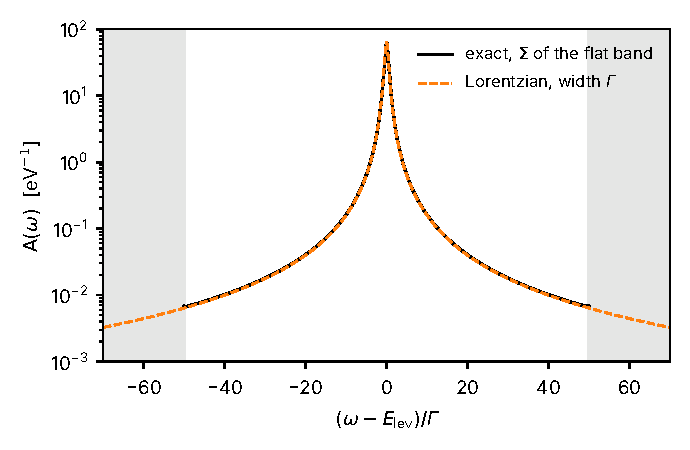
\includegraphics[width=0.68\linewidth]{figures/ch04/fig4_8b.pdf}
  \caption{Spectral function of a level of energy $E_{\mathrm{lev}}$ coupled to a flat band of width $E_{\mathrm{w}} = \SI{1}{eV}$ centered on $E_{\mathrm{lev}}$, with golden-rule rate $\varGamma = \SI{10}{meV}$ (the model of \cref{we:4-level}), on a logarithmic scale against $(\omega - E_{\mathrm{lev}})/\varGamma$. Solid: exact result, $\SpecA_{dd} = -\pi^{-1}\Imag[\omega - E_{\mathrm{lev}} - \Sigma^{\mathrm{R}}_d(\omega)]^{-1}$ with the self-energy of the band in the limit of a continuum, $\Sigma^{\mathrm{R}}_d = (\varGamma/2\pi)\ln[(\omega - E_{\mathrm{lev}} + E_{\mathrm{w}}/2)/(\omega - E_{\mathrm{lev}} - E_{\mathrm{w}}/2)]$ at $\omega + \ii0^+$. Dashed: Lorentzian of full width $\varGamma$ and unit weight. Shaded: outside the band, where the exact function vanishes (its two bound states lie exponentially close to the band edges and carry negligible weight) and the Lorentzian has the weight $2\varGamma/(\pi E_{\mathrm{w}}) = 0.0064$. Inside the band the exact function exceeds the Lorentzian by 1.0 percent at $|\omega - E_{\mathrm{lev}}| = \varGamma$ and by 1.3 percent at $10\varGamma$, because its quasiparticle residue is $1.0064$.}
  \label{fig:4-level}
\end{figure}

\subsection{Imaginary time}

At finite temperature two exponentials of the Hamiltonian appear in every average: $\ee^{-\ii H_\mu t}$ moves the operators in time, and $\ee^{-\beta H_\mu}$ weights the states. The second is the first at the imaginary time $t = -\ii\beta$. Matsubara used this to treat both on the same footing~\cite{matsubara1955new}. Define operators in imaginary time $\tau$ by
\begin{equation*}
  O(\tau) = \ee^{\tau H_\mu}\,O\,\ee^{-\tau H_\mu}, \qquad 0 \le \tau \le \beta ,
\end{equation*}
which is the Heisenberg operator $O(t)$ at $t = -\ii\tau$. Note that $c^\dagger(\tau)$ is not the adjoint of $c(\tau)$. The imaginary-time, or Matsubara, Green's function is
\begin{equation}
  \GF(\vect{k},\tau) = -\bigl\langle\mathrm{T}_\tau\,c_{\vect{k}}(\tau)\,c^\dagger_{\vect{k}}(0)\bigr\rangle ,
  \label{eq:4.7-Gtau}
\end{equation}
where $\mathrm{T}_\tau$ puts the operator with the larger $\tau$ on the left, with a minus sign for an exchange of fermion operators. Its use is that a perturbation expansion of $\ee^{-\beta H_\mu}$ and of $\ee^{\pm\tau H_\mu}$ in $H_{\mathrm{int}}$ is one Dyson series along the imaginary-time axis, with the same structure as \cref{eq:2.4-dyson}, and Wick's theorem then reduces every term to products of free Green's functions (\cref{sec:4.8}). The real-time time-ordered function of \cref{eq:4.7-GT}, however, has no expansion of this single-exponential form at $T > 0$ (\cref{app:D.11}), which is why the Matsubara function replaces it.

The cyclic property of the trace makes \cref{eq:4.7-Gtau} antiperiodic, $\GF(\vect{k},\tau - \beta) = -\GF(\vect{k},\tau)$ for $0 < \tau < \beta$ (\cref{app:D.10}). A function on $-\beta < \tau < \beta$ with this property is a Fourier series in the odd multiples of $\pi T$, the fermionic Matsubara frequencies $\omega^{\mathrm{F}}_j = (2j + 1)\pi T$ with integer $j$:
\begin{equation}
  \GF(\vect{k},\ii\omega^{\mathrm{F}}_j) = \int_0^\beta\dd\tau\,\ee^{\ii\omega^{\mathrm{F}}_j\tau}\,\GF(\vect{k},\tau), \qquad
  \GF(\vect{k},\tau) = T\sum_j\ee^{-\ii\omega^{\mathrm{F}}_j\tau}\,\GF(\vect{k},\ii\omega^{\mathrm{F}}_j) .
  \label{eq:4.7-Gmats}
\end{equation}
A correlation of two operators that each change the electron number by an even amount, such as two densities, is periodic instead, and its series runs over the bosonic frequencies $\omega^{\mathrm{B}}_j = 2j\pi T$. As $T \to 0$ both sets become dense on the imaginary axis.

The Lehmann form follows as before. For $0 < \tau < \beta$ only the ordering $c_{\vect{k}}(\tau)c^\dagger_{\vect{k}}$ appears, and inserting states leads to $\GF(\vect{k},\tau) = -\sum_{i,f}p_i|\langle f|c^\dagger_{\vect{k}}|i\rangle|^2\,\ee^{-(E_f - E_i)\tau}$. The integral in \cref{eq:4.7-Gmats} is elementary, and $\ee^{\ii\omega^{\mathrm{F}}_j\beta} = -1$:
\begin{equation*}
  \int_0^\beta\dd\tau\,\ee^{[\ii\omega^{\mathrm{F}}_j - (E_f - E_i)]\tau} = -\frac{1 + \ee^{-\beta(E_f - E_i)}}{\ii\omega^{\mathrm{F}}_j - (E_f - E_i)} .
\end{equation*}
Since $p_i\,\ee^{-\beta(E_f - E_i)} = p_f$, the weight becomes $(p_i + p_f)|\langle f|c^\dagger_{\vect{k}}|i\rangle|^2$, and the relabeling that led to \cref{eq:4.7-occ} shows that this is the weight of the spectral function at $\omega = E_f - E_i$.
\begin{keyresult}[Matsubara Green's function and analytic continuation]
\begin{equation}
  \GF(\vect{k},\ii\omega^{\mathrm{F}}_j) = \int\dd\omega'\,\frac{\SpecA(\vect{k},\omega')}{\ii\omega^{\mathrm{F}}_j - \omega'}, \qquad
  \GF^{\mathrm{R}}(\vect{k},\omega) = \GF(\vect{k},\ii\omega^{\mathrm{F}}_j \to \omega + \ii0^+) .
  \label{eq:4.7-continuation}
\end{equation}
The Matsubara and retarded functions are values of one analytic function, $\int\dd\omega'\,\SpecA(\vect{k},\omega')/(z - \omega')$, at the points $z = \ii\omega^{\mathrm{F}}_j$ and just above the real axis.
\end{keyresult}
In practice a Matsubara function computed in closed form is turned into the retarded one by the substitution $\ii\omega^{\mathrm{F}}_j \to \omega + \ii0^+$, made after every factor $\ee^{\ii\beta\omega^{\mathrm{F}}_j}$ has been replaced by $-1$. The continuation is unique, because the function falls off at large $|z|$ (\cref{app:C.5})~\cite{baym1961determination}. The Dyson equation carries over with the same self-energy evaluated at $z = \ii\omega^{\mathrm{F}}_j$, $\GF(\vect{k},\ii\omega^{\mathrm{F}}_j) = [\ii\omega^{\mathrm{F}}_j - \xi_{\vect{k}} - \Sigma(\vect{k},\ii\omega^{\mathrm{F}}_j)]^{-1}$, and for free electrons $\GF_0(\vect{k},\ii\omega^{\mathrm{F}}_j) = 1/(\ii\omega^{\mathrm{F}}_j - \xi_{\vect{k}})$.

Diagrams return their results as sums over Matsubara frequencies, and these are done by contour integration. The occupation is the simplest case. At $\tau = 0^-$ the time ordering puts $c^\dagger_{\vect{k}}$ on the left, $\GF(\vect{k},0^-) = \langle c^\dagger_{\vect{k}}c_{\vect{k}}\rangle$, and by \cref{eq:4.7-Gmats}
\begin{equation}
  \langle c^\dagger_{\vect{k}}c_{\vect{k}}\rangle = T\sum_j\ee^{\ii\omega^{\mathrm{F}}_j0^+}\,\GF(\vect{k},\ii\omega^{\mathrm{F}}_j) .
  \label{eq:4.7-occmats}
\end{equation}
The Fermi function $n_{\mathrm{F}}(z)$ has poles at the points $z = \ii\omega^{\mathrm{F}}_j$, each with residue $-T$, and the sum is a contour integral of $n_{\mathrm{F}}(z)\,\GF(\vect{k},z)$ around small circles that enclose them (\cref{fig:4-matsubara}a). Opened up, the circles become two lines that run along the real axis, above and below the cut of $\GF(\vect{k},z)$ (\cref{fig:4-matsubara}b). The jump of $\GF$ across the cut is $-2\pi\ii\SpecA$, by \cref{eq:4.7-lehmann}, and the sum becomes $\int\dd\omega\,\SpecA(\vect{k},\omega)\,n_{\mathrm{F}}(\omega)$, the occupation \cref{eq:4.7-occ}. \Cref{app:D.10} writes out the steps and the sum of two propagators that appears in every bubble diagram.

\begin{figure}[tbp]
  \centering
  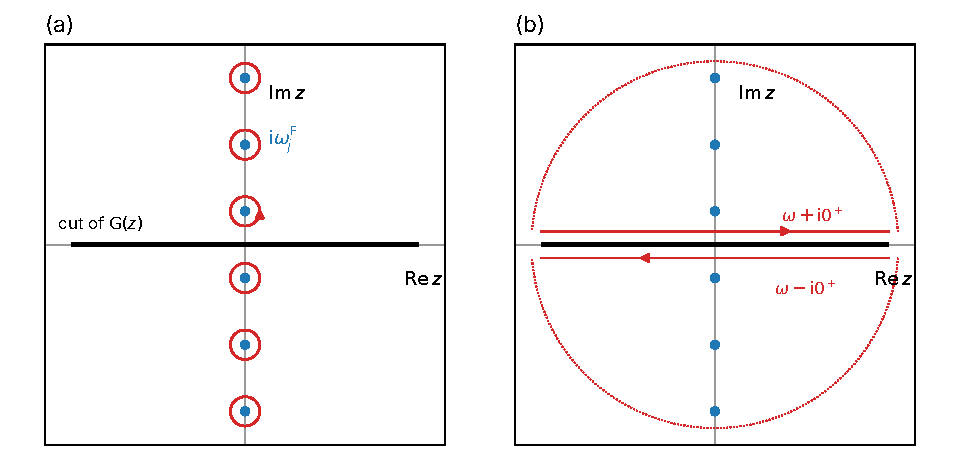
\includegraphics[width=\linewidth]{figures/ch04/fig4_8.pdf}
  \caption{Frequency sums by contour integration in the complex frequency plane $z$. (a) The fermionic Matsubara frequencies $\ii\omega^{\mathrm{F}}_j = (2j + 1)\pi\ii T$ (dots) are the poles of the Fermi function $n_{\mathrm{F}}(z)$, each with residue $-T$. A sum $T\sum_jg(\ii\omega^{\mathrm{F}}_j)$ is minus the integral of $n_{\mathrm{F}}(z)\,g(z)/2\pi\ii$ around small circles that enclose them counterclockwise. For $g = \GF(\vect{k},z)$ the only other singularity is the cut on the real axis (thick line), where the spectral function is nonzero. (b) The circles are merged into the boundaries of the upper and lower half planes: a line just above the real axis, at $\omega + \ii0^+$, run from left to right, and a line just below, at $\omega - \ii0^+$, run from right to left. The large arcs (dotted) contribute nothing when $n_{\mathrm{F}}(z)\,g(z)$ falls off faster than $1/|z|$ in every direction. The two lines see the retarded and advanced functions, and their difference, $-2\pi\ii\SpecA$, turns the sum into an integral over real frequencies.}
  \label{fig:4-matsubara}
\end{figure}

\subsection{The density response in imaginary time}

The density response obeys the same rules. For two operators $O_a$, $O_b$ that conserve the electron number, define
\begin{equation}
  R_{ab}(\vect{q},\tau) = -\frac{1}{\Vol}\bigl\langle\mathrm{T}_\tau\,O_a(\vect{q},\tau)^\dagger\,O_b(\vect{q},0)\bigr\rangle ,
  \label{eq:4.7-Rtau}
\end{equation}
with $O_a(\vect{q},\tau)^\dagger$ meaning $\ee^{\tau H_\mu}O_a(\vect{q})^\dagger\ee^{-\tau H_\mu}$ and no sign on exchange, since the operators are bosonic. The function is periodic in $\tau$ with period $\beta$, and its coefficients are taken at $\ii\omega^{\mathrm{B}}_j$. For $0 < \tau < \beta$ it is $-\Vol^{-1}\sum_{i,f}p_i\langle i|O_a^\dagger|f\rangle\langle f|O_b|i\rangle\,\ee^{-(E_f - E_i)\tau}$. Integrated with $\ee^{\ii\omega^{\mathrm{B}}_j\tau}$, now with $\ee^{\ii\omega^{\mathrm{B}}_j\beta} = +1$, each term gives $[\ee^{-\beta(E_f - E_i)} - 1]/[\ii\omega^{\mathrm{B}}_j - (E_f - E_i)]$ if the denominator is nonzero, and $\beta$ if it is zero, which happens only for $j = 0$ and $E_f = E_i$. With $p_i\,\ee^{-\beta(E_f - E_i)} = p_f$,
\begin{equation}
  R_{ab}(\vect{q},\ii\omega^{\mathrm{B}}_j) = \frac{1}{\Vol}\sum_{i,f}^{E_f \ne E_i}\frac{(p_i - p_f)\,\langle i|O_a^\dagger|f\rangle\langle f|O_b|i\rangle}{\ii\omega^{\mathrm{B}}_j - (E_f - E_i)}
  - \delta_{j0}\,\frac{\beta}{\Vol}\sum_{i,f}^{E_f = E_i}p_i\,\langle i|O_a^\dagger|f\rangle\langle f|O_b|i\rangle .
  \label{eq:4.7-Rmats}
\end{equation}
In the retarded Lehmann form \cref{eq:4.1-lehmann}, relabeling $i \leftrightarrow f$ in the antiresonant term turns its weight into $-p_f\langle i|O_a^\dagger|f\rangle\langle f|O_b|i\rangle$ and its denominator into $\omega - (E_f - E_i) + \ii0^+$, and the two terms combine into $(p_i - p_f)$ times one pole. That is the sum in \cref{eq:4.7-Rmats} with $\ii\omega^{\mathrm{B}}_j \to \omega + \ii0^+$.
\begin{keyresult}[Response function from imaginary time]
\begin{equation}
  R_{ab}(\vect{q},\omega) = R_{ab}(\vect{q},\ii\omega^{\mathrm{B}}_j \to \omega + \ii0^+), \qquad j > 0 .
  \label{eq:4.7-Rcont}
\end{equation}
The retarded response function of \cref{sec:4.1} is the analytic continuation of the imaginary-time correlation function \cref{eq:4.7-Rtau} from the positive bosonic Matsubara frequencies.
\end{keyresult}
The term with $\delta_{j0}$ is not part of the continuation, which uses the points $j > 0$ alone, and it has a physical meaning. It comes from matrix elements between states of equal energy, and it is the extra term proportional to $\beta$ that distinguishes the isothermal static response from the limit $\omega \to 0$ of $R_{ab}(\vect{q},\omega)$, the isolated response of \cref{sec:4.1}~\cite{kubo1957statistical}. The value at $\omega^{\mathrm{B}}_0 = 0$ is the isothermal one, since it is a derivative of an equilibrium average in which the field has been present long enough for the target to stay in equilibrium with the bath.

For independent electrons the imaginary-time route writes the response as a sum over one fermionic frequency of a product of two free Green's functions. With $O_a = O_b = n_e(\vect{q})$ from \cref{eq:2.3-nq} and occupations $n_{\mathrm{F}}(\xi_{\vect{k}})$, \cref{app:D.10} evaluates \cref{eq:4.7-Rtau} directly and shows that it equals
\begin{equation}
  R^0(\vect{q},\ii\omega^{\mathrm{B}}_j) = \frac{1}{\Vol}\sum_{\vect{k}}T\sum_{j'}\GF_0(\vect{k},\ii\omega^{\mathrm{F}}_{j'})\,\GF_0(\vect{k} + \vect{q},\ii\omega^{\mathrm{F}}_{j'} + \ii\omega^{\mathrm{B}}_j)
  = \frac{1}{\Vol}\sum_{\vect{k}}\frac{n_{\mathrm{F}}(\xi_{\vect{k}}) - n_{\mathrm{F}}(\xi_{\vect{k}+\vect{q}})}{\ii\omega^{\mathrm{B}}_j + \xi_{\vect{k}} - \xi_{\vect{k}+\vect{q}}} ,
  \label{eq:4.7-bubble}
\end{equation}
with the sum over $\vect{k}$ including spin. Continued to $\omega + \ii0^+$, it is the independent-electron response whose imaginary part is the transition sum \cref{eq:2.5-indep}, and \cref{sec:4.5} evaluates it for the electron gas. The product of two propagators, one carrying the electron from $\vect{k}$ to $\vect{k} + \vect{q}$ and one carrying the hole back, is the bubble diagram of \cref{sec:4.8}. With interactions the same continuation holds term by term, and the diagrams of the next section compute $\Sigma$ and $R$ as Matsubara sums, which \cref{eq:4.7-continuation,eq:4.7-Rcont} then carry to the real frequencies at which a dark-matter particle deposits its energy.

\section{Feynman diagrams}\label{sec:4.8}

An electron injected \SI{5}{eV} above the conduction-band edge of silicon does not stay there for long. It knocks electrons across the gap and emits phonons, and its quasiparticle peak acquires the width $\varGamma_{\mathrm{qp}} = -2z_{\mathrm{qp}}\Imag\Sigma^{\mathrm{R}}$ of \cref{eq:4.7-qp}. To get a number we need $\Sigma$, and the self-energy of an interacting system can only be computed as a series in the interaction. The same is true of the density response beyond the independent-electron bubble of \cref{sec:4.5}. Feynman diagrams are the bookkeeping for these series: each term of the expansion is a picture, and a small set of rules turns the picture into an integral. The treatment follows Refs.~\cite{bruus2004many}, \cite[Chaps.~3 and 7]{fetter1971quantum} and \cite[Chaps.~2 and 3]{mahan2000many}.

\subsection{Wick's theorem and the rules}

Split $H_\mu = H_0 + H_{\mathrm{int}}$, with $H_0 = \sum_{\vect{k}}\xi_{\vect{k}}c^\dagger_{\vect{k}}c_{\vect{k}}$ the independent electrons of \cref{sec:4.7}. In imaginary time the Boltzmann factor and the Heisenberg operators can both be written with the ordered exponential $U_{\mathrm{I}}(\beta,0) = \mathrm{T}_\tau\exp[-\int_0^\beta\dd\tau\,H_{\mathrm{int},\mathrm{I}}(\tau)]$, where the subscript I marks operators that evolve with $H_0$ alone. The Matsubara Green's function \cref{eq:4.7-Gtau} becomes the ratio \cref{eq:D.11-Gexp},
\begin{equation*}
  \GF(\vect{k},\tau) = -\frac{\bigl\langle\mathrm{T}_\tau\,U_{\mathrm{I}}(\beta,0)\,c_{\vect{k},\mathrm{I}}(\tau)\,c^\dagger_{\vect{k},\mathrm{I}}(0)\bigr\rangle_0}{\bigl\langle U_{\mathrm{I}}(\beta,0)\bigr\rangle_0} ,
\end{equation*}
with $\langle\cdots\rangle_0$ the average in the free grand-canonical state. Expanding the exponential, the term of order $n$ in $H_{\mathrm{int}}$ is an integral over $n$ imaginary times of a free average of a time-ordered string of creation and annihilation operators. Nothing has been approximated so far.

Wick's theorem evaluates these averages~\cite{wick1950evaluation}. In the free state, the time-ordered average of a string of fermion operators is a sum over all ways of grouping the operators into pairs. Each grouping contributes the product of its pair averages, with the sign of the permutation that brings the members of every pair next to each other. Only pairs of one creation and one annihilation operator of the same mode survive. Their time-ordered averages, the contractions, are free Green's functions:
\begin{equation}
  \bigl\langle\mathrm{T}_\tau\,c_{\vect{k},\mathrm{I}}(\tau)\,c^\dagger_{\vect{k},\mathrm{I}}(\tau')\bigr\rangle_0 = -\GF_0(\vect{k},\tau - \tau') .
  \label{eq:4.8-contract}
\end{equation}
For bosons the same holds without signs, and a contraction of the field $d_{\vect{Q}} + d^\dagger_{-\vect{Q}}$ with itself is the free boson propagator. The theorem is the quantum version of the statement that every moment of a Gaussian distribution is a sum over pairings (\cref{app:C.6}): the free grand-canonical state is the ``Gaussian'' state of the many-body problem. \Cref{app:D.11} proves it with Gaudin's trace argument~\cite{gaudin1960demonstration}, which uses only the anticommutators and the cyclic property of the trace. At $T = 0$ the same theorem holds for averages in the Fermi sea $|\Phi_0\rangle$, the limit $\beta \to \infty$ of the free state, with the contraction $\ii\GF_0(\vect{k},t - t')$ of the time-ordered function \cref{eq:4.7-GT}. The interacting ground state is reached from $|\Phi_0\rangle$ by switching on the interaction slowly, as long as no level crossing intervenes (the theorem of Gell-Mann and Low~\cite{gellmann1951bound}), and the real-time expansion \cref{eq:D.11-GT} has the same structure.

Each pairing is drawn as a picture. A contraction \cref{eq:4.8-contract} is a solid line with an arrow, from the point where the electron is created to the point where it is annihilated. A factor $H_{\mathrm{int}}$ is a vertex, or for the Coulomb interaction a dashed line whose two ends are the two density operators of the pair interaction. Pairings that fall into a piece attached to the external points and a piece that is not, the vacuum diagrams, cancel against the denominator, which is the linked-cluster theorem, and only connected diagrams remain. Relabeling the $n$ identical interaction factors, and exchanging the two ends of each line, produces $n!\,2^n$ pairings with the same value, which cancel the $1/n!$ of the exponential and the $\tfrac12$ of the pair interaction. Collecting the signs and the factors of $T$ and $\Vol$, \cref{app:D.11} arrives at the following rules.
\begin{keyresult}[Feynman rules in imaginary time]
The Green's function $\GF(\vect{k},\ii\omega^{\mathrm{F}}_j)$ is the sum of all connected, topologically distinct diagrams with two external points, each evaluated with the following factors.
\begin{enumerate}
  \item Each solid line carrying $(\vect{p},\ii\omega^{\mathrm{F}})$ is $\GF_0(\vect{p},\ii\omega^{\mathrm{F}}) = 1/(\ii\omega^{\mathrm{F}} - \xi_{\vect{p}})$; spin is conserved along it.
  \item Each Coulomb line carrying $(\vect{k},\ii\omega^{\mathrm{B}})$ is $-v_{\mathrm{C}}(k)/\Vol$. Each boson line is $-|g(\vect{Q})|^2\mathsf{D}_0(\vect{Q},\ii\omega^{\mathrm{B}})/\Vol$, with $\mathsf{D}_0(\vect{Q},\ii\omega^{\mathrm{B}}) = 2\omega_{\vect{Q}}/[(\ii\omega^{\mathrm{B}})^2 - \omega_{\vect{Q}}^2]$ for a boson of energy $\omega_{\vect{Q}}$ coupled through $H_{\mathrm{int}} = \Vol^{-1/2}\sum g(\vect{Q})\,c^\dagger_{\vect{k}+\vect{Q}}c_{\vect{k}}(d_{\vect{Q}} + d^\dagger_{-\vect{Q}})$.
  \item Momentum and frequency are conserved at every vertex. Each independent internal momentum is summed, and each independent internal frequency carries $T\sum_j$.
  \item Each closed fermion loop gives $-1$ and a sum over its spin.
  \item A solid line that begins and ends on the same interaction carries $\ee^{\ii\omega^{\mathrm{F}}0^+}$.
\end{enumerate}
The response function \cref{eq:4.7-Rtau} of two densities is $-1/\Vol$ times the sum of connected diagrams with two density vertices, at which $\vect{q}$ and $\ii\omega^{\mathrm{B}}_j$ enter and leave, evaluated with the same rules. At $T = 0$ the rules for the time-ordered functions are the same with $\GF_0(\vect{p},\omega) = 1/(\omega - \xi_{\vect{p}} + \ii0^+\operatorname{sgn}\xi_{\vect{p}})$, each Coulomb line $+\ii v_{\mathrm{C}}(k)/\Vol$, and each internal frequency $\int\dd\omega/2\pi$, and the time-ordered response $-(\ii/\Vol)\langle\mathrm{T}\,O_a(\vect{q},t)^\dagger O_b(\vect{q},0)\rangle$ carries $+\ii/\Vol$ in place of $-1/\Vol$.
\end{keyresult}
The sign of a loop is the one rule that has no counterpart in the old-fashioned perturbation theory of \cref{sec:2.4}. It comes from the last contraction around the loop, which pairs the first creation operator with the last annihilation operator and costs an odd number of exchanges. The rule for the response function needs one line of its own. The definition \cref{eq:4.7-Rtau} carries $-1/\Vol$. A response diagram has $2n + 2$ propagators at order $n$, an even number, so the $-1$ of each contraction drops out. The signs left over are those of the expansion, $(-1)^n$, which the rule puts into the lines, and of the loops. \Cref{app:D.11} checks the rules for $\GF$ at first order against the Hartree--Fock self-energy. The next subsection checks the rule for $R$ against \cref{eq:4.7-bubble} and against the screening of \cref{sec:4.4}.

In the frequency representation every line is a simple pole, every frequency sum is done by the residue formula \cref{eq:C.5-matsum}, and the temperature enters only through these sums: $\GF_0$ and $\mathsf{D}_0$ do not depend on it, and the occupation factors $n_{\mathrm{F}}$ and $n_{\mathrm{B}}$ appear as residues of $n_{\mathrm{F}}(z)$ and $n_{\mathrm{B}}(z)$.

\subsection{The bubble and the random-phase chain}

The density response of independent electrons is the simplest diagram there is: one fermion loop through the two density vertices (\cref{fig:4-diagrams}a). An electron is created in $\vect{k} + \vect{q}$ and a hole in $\vect{k}$ at one vertex, and both are annihilated at the other. By the rules, the loop contributes $-1$ and a spin sum, the two lines give $\GF_0(\vect{k},\ii\omega^{\mathrm{F}}_{j'})\GF_0(\vect{k}+\vect{q},\ii\omega^{\mathrm{F}}_{j'} + \ii\omega^{\mathrm{B}}_j)$, and the internal momentum and frequency are summed. With the $-1/\Vol$ of the response,
\begin{equation}
  R^0(\vect{q},\ii\omega^{\mathrm{B}}_j) = \frac1\Vol\sum_{\vect{k}s}T\sum_{j'}\GF_0(\vect{k},\ii\omega^{\mathrm{F}}_{j'})\,\GF_0(\vect{k}+\vect{q},\ii\omega^{\mathrm{F}}_{j'} + \ii\omega^{\mathrm{B}}_j) ,
  \label{eq:4.8-bubble}
\end{equation}
which is the first form of \cref{eq:4.7-bubble}. The frequency sum is \cref{eq:D.10-sum}, and it produces the Pauli difference $[n_{\mathrm{F}}(\xi_{\vect{k}}) - n_{\mathrm{F}}(\xi_{\vect{k}+\vect{q}})]/(\ii\omega^{\mathrm{B}}_j + \xi_{\vect{k}} - \xi_{\vect{k}+\vect{q}})$. Continued to $\omega + \ii0^+$ by \cref{eq:4.7-Rcont}, this is the independent-electron response \cref{eq:4.5-R0}, whose evaluation for the electron gas is the Lindhard function of \cref{sec:4.5}. In a crystal the plane waves become Bloch states $\psi_{n\vect{k}}$, the density vertex $n_e(\vect{q}+\vect{G})$ acquires the matrix element $\rho_{mn}(\vect{k},\vect{q}+\vect{G})$ between the two states it connects, and the same diagram is the crystal bubble \cref{eq:4.6-R0} (\cref{eq:D.12-R,eq:D.12-L0}). The sign of the rule passes its first test: the static bubble is negative, as a response must be.

\begin{figure}[tbp]
  \centering
  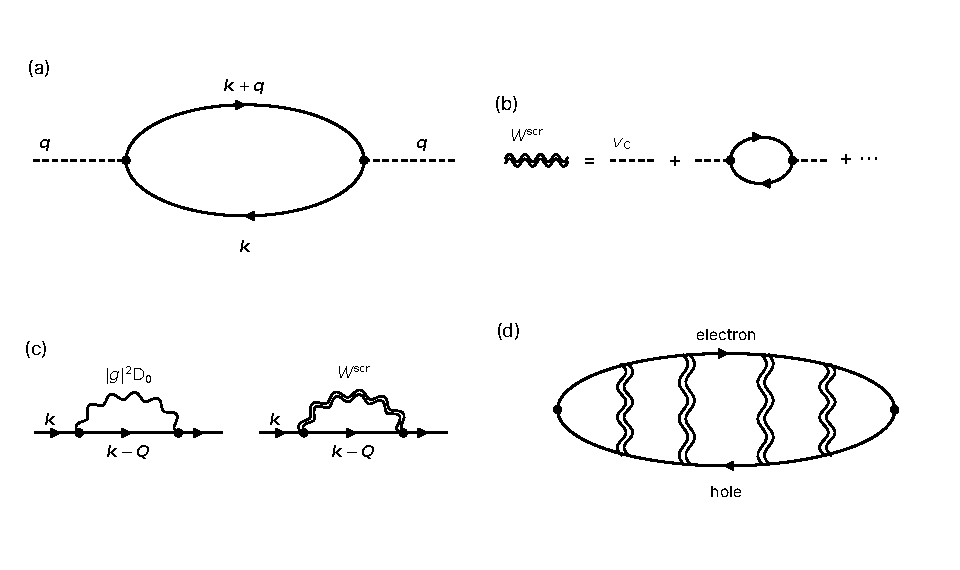
\includegraphics[width=\linewidth]{figures/ch04/fig4_9.pdf}
  \caption{The diagrams of \cref{sec:4.8}. Solid lines with arrows are free electron propagators $\GF_0$; an arrow against the direction of the momentum label is a hole. Dashed lines are the bare Coulomb interaction $v_{\mathrm{C}}$, except the short dashed stubs in (a), which mark the external momentum $\vect{q}$ entering and leaving at the density vertices; single wavy lines a boson, double wavy lines the screened interaction $W^{\mathrm{scr}}$. Dots are vertices. (a) The bubble: a density vertex creates an electron in $\vect{k}+\vect{q}$ and a hole in $\vect{k}$, and a second vertex annihilates them; it is the independent-electron response $R^0$. (b) The screened interaction as the random-phase chain of bubbles joined by Coulomb lines, $W^{\mathrm{scr}} = v_{\mathrm{C}} + v_{\mathrm{C}}R^0v_{\mathrm{C}} + \cdots$. (c) The self-energy of an electron that emits and reabsorbs a boson, with the line $|g|^2\mathsf{D}_0$, and the $GW$ self-energy, the same diagram with the screened line. (d) The ladder: the electron and the hole of the bubble interact through screened interaction lines. Summed together with the chain of exchange lines, it becomes the Bethe--Salpeter equation of \cref{sec:4.9}.}
  \label{fig:4-diagrams}
\end{figure}

At first order in $v_{\mathrm{C}}$ the bubble is corrected by three kinds of diagram, which differ in where the Coulomb line attaches. It can join two bubbles, the line carrying the momentum $\vect{q}$ from one to the other. It can run across the bubble, from the electron line to the hole line. Or it can begin and end on one propagator, which is a first-order self-energy inserted into that line. The first kind has two loops, and by the rules its value is $-(1/\Vol)(-1)^2(-v_{\mathrm{C}}(q)/\Vol)\,(\Vol R^0)(\Vol R^0) = R^0v_{\mathrm{C}}(q)R^0$, with a plus sign, where each loop without its sign is $\sum_{\vect{k}s}T\sum_{j'}\GF_0\GF_0 = \Vol R^0$. The second kind has the same propagators and the same line but only one loop, and the opposite sign. Repeating the first kind gives the chain $R^0 + R^0v_{\mathrm{C}}R^0 + R^0v_{\mathrm{C}}R^0v_{\mathrm{C}}R^0 + \cdots$, a geometric series with the sum
\begin{equation}
  R = \frac{R^0}{1 - v_{\mathrm{C}}(q)R^0} .
  \label{eq:4.8-chain}
\end{equation}
This is the random-phase approximation \cref{eq:4.5-rpa}, now as a definite selection of diagrams: the chain of bubbles, and nothing inside them. Its sign is the one \cref{sec:4.4} found from the classical argument, $\varepsilon = 1 - v_{\mathrm{C}}R^0 > 1$ in the static limit. The general statement is just as direct. A diagram for $R$ either can or cannot be cut into two by cutting a single Coulomb line at the momentum $\vect{q}$. Call the sum of those that cannot the proper part $\tilde R$. Every diagram that can is a chain of proper pieces joined by such lines, and the sum of the chains is $R = \tilde R + \tilde Rv_{\mathrm{C}}R$, the Dyson equation \cref{eq:4.4-dyson}. The blobs of \cref{fig:4-series} are sums of Feynman diagrams, and the random-phase approximation keeps the bubble alone in each blob.

In a crystal the Coulomb line between two bubbles carries $\vect{q} + \vect{G}$ for every reciprocal-lattice vector $\vect{G}$, and the chain becomes the matrix equation of \cref{sec:4.6}. The line with $\vect{G} = 0$ carries the macroscopic field. The lines with $\vect{G} \ne 0$ are the local fields, and in the language of transitions they form the exchange kernel $K^{\mathrm{x}}$ of \cref{sec:4.6}, the Coulomb interaction without its $\vect{G} = 0$ term. The second kind of first-order diagram, the line across the bubble, is the attraction between the electron and the hole that the chain leaves out. Repeated, with each interaction line screened by its own chain of bubbles, it forms the ladder of \cref{fig:4-diagrams}d. The sum of ladders and exchange chains is the Bethe--Salpeter equation, the equation for an electron--hole pair that propagates while the two particles attract each other, and its bound states are the excitons of \cref{sec:4.9}. \Cref{app:D.12} derives it from these diagrams, with the direct kernel $K^{\mathrm{d}}$ built from the screened interaction line.

\subsection{Reducible lines and the thermodynamic limit}\label{sec:4.8-removal}

The f-sum rule for $\varepsilon_2$ in \cref{sec:4.4} rested on one claim. Deleting the Coulomb interaction at the single wavevector $\vect{q}$ from the Hamiltonian leaves the equilibrium state unchanged in the thermodynamic limit, while it turns the full response into its proper part. Diagrams make both halves precise. Let $\bar H$ be $H$ with the Coulomb terms at $\pm\vect{q}$ removed, $\vect{q} \ne 0$, and compare the diagrams of the two Hamiltonians.

Take first any equilibrium average: the Green's function at some $\vect{k}$, an occupation, or the free energy per volume. In its diagrams a Coulomb line has its momentum fixed by conservation only if cutting it separates the diagram into two pieces. The piece without external points then exchanges no momentum with the rest, and the line carries $\vect{k} = 0$, which is absent in a neutral system. Every other line carries a loop momentum, summed as $\Vol^{-1}\sum_{\vect{k}}$ with $v_{\mathrm{C}}(k)$ finite at $\vect{k} = \pm\vect{q}$. Deleting the two terms $\vect{k} = \pm\vect{q}$ from such a sum changes it by a relative amount of order $1/N$, with $N$ the number of electrons, and it vanishes in the thermodynamic limit. The equilibrium state of $\bar H$ is therefore that of $H$, at every order.

Now take the response at $\vect{q}$. Here a line can carry exactly $\vect{q}$, and conservation forces it to when, and only when, the line is a bridge: cutting it splits the diagram into a piece attached to one density vertex and a piece attached to the other. These are the lines of the chain. In $\bar H$ they are gone, while the lines at $\pm\vect{q}$ inside loops lose a negligible term as before.
\begin{keyresult}[Removing one Fourier component]
In the thermodynamic limit, the Hamiltonian $\bar H$ without the Coulomb terms at $\pm\vect{q}$ has the same equilibrium state as $H$, and its density response at $\vect{q}$ is the proper part of the response of $H$,
\begin{equation}
  \bar R(\vect{q},\omega) = \tilde R(\vect{q},\omega) .
  \label{eq:4.8-removal}
\end{equation}
In a crystal the same argument with the $\vect{G} = 0$ term alone removed identifies $\bar R$ of \cref{app:D.7} with the response that is proper with respect to the macroscopic line only.
\end{keyresult}
Because $\bar R$ is the response function of a Hamiltonian in its own equilibrium state, every exact property proved in \cref{sec:4.1,sec:4.2,sec:4.3} holds for it: the Lehmann form, positivity of the absorption and the f-sum rule with the same density $\nd_e$. That is what \cref{sec:4.4} used for $\varepsilon_2$ and for the Ward identity of the proper current response. The argument is diagrammatic, and it holds at every order of perturbation theory for $\vect{q} \ne 0$. At $\vect{q} \to 0$ the deleted terms are at the edge of the sum and the limit is taken after the thermodynamic one, which is the order in which the optical limit of \cref{app:D.7} is defined.

\subsection{An electron coupled to a boson}

An electron in a crystal shakes the lattice as it moves: it emits a phonon, propagates in a different state, and absorbs the phonon again. The lowest self-energy diagram of this process is the Fock diagram with a boson line (\cref{fig:4-diagrams}c), second order in the coupling $g$. It carries every feature of finite-temperature perturbation theory in a few lines, and \cref{sec:6.3} builds the electron--phonon self-energy of silicon on it. By the rules, with the boson line carrying $(\vect{Q},\ii\omega^{\mathrm{B}}_{j'})$ and the electron line $(\vect{k} - \vect{Q},\ii\omega^{\mathrm{F}}_j - \ii\omega^{\mathrm{B}}_{j'})$, and no loop,
\begin{equation*}
  \Sigma(\vect{k},\ii\omega^{\mathrm{F}}_j) = -\frac1\Vol\sum_{\vect{Q}}|g(\vect{Q})|^2\,T\sum_{j'}\mathsf{D}_0(\vect{Q},\ii\omega^{\mathrm{B}}_{j'})\,\GF_0(\vect{k} - \vect{Q},\ii\omega^{\mathrm{F}}_j - \ii\omega^{\mathrm{B}}_{j'}) .
\end{equation*}
The sum runs over a bosonic frequency, and by \cref{eq:C.5-matsum} it is minus the sum of the residues of $n_{\mathrm{B}}(z)h(z)$ at the poles of
\begin{equation*}
  h(z) = \Bigl[\frac{1}{z - \omega_{\vect{Q}}} - \frac{1}{z + \omega_{\vect{Q}}}\Bigr]\frac{1}{\ii\omega^{\mathrm{F}}_j - z - \xi'} , \qquad \xi' = \xi_{\vect{k}-\vect{Q}} ,
\end{equation*}
which falls off as $1/|z|^3$, so no convergence factor is needed. The pole at $z = \omega_{\vect{Q}}$ has the residue $n_{\mathrm{B}}(\omega_{\vect{Q}})/(\ii\omega^{\mathrm{F}}_j - \xi' - \omega_{\vect{Q}})$. The pole at $z = -\omega_{\vect{Q}}$ has the residue $-n_{\mathrm{B}}(-\omega_{\vect{Q}})/(\ii\omega^{\mathrm{F}}_j - \xi' + \omega_{\vect{Q}})$, and $n_{\mathrm{B}}(-x) = -1 - n_{\mathrm{B}}(x)$ turns its numerator into $1 + n_{\mathrm{B}}$. The pole at $z = \ii\omega^{\mathrm{F}}_j - \xi'$, where the electron line is singular, has the residue $-n_{\mathrm{B}}(\ii\omega^{\mathrm{F}}_j - \xi')\,\mathsf{D}_0(\ii\omega^{\mathrm{F}}_j - \xi')$. Before anything is continued, the Bose function at a fermionic frequency is simplified with $\ee^{\ii\beta\omega^{\mathrm{F}}_j} = -1$: $n_{\mathrm{B}}(\ii\omega^{\mathrm{F}}_j - \xi') = 1/(-\ee^{-\beta\xi'} - 1) = -[1 - n_{\mathrm{F}}(\xi')]$. This residue is then $[1 - n_{\mathrm{F}}(\xi')][1/(\ii\omega^{\mathrm{F}}_j - \xi' - \omega_{\vect{Q}}) - 1/(\ii\omega^{\mathrm{F}}_j - \xi' + \omega_{\vect{Q}})]$. Adding the three residues, changing the sign, and multiplying by $-|g|^2/\Vol$ gives the self-energy.
\begin{keyresult}[Second-order self-energy with a boson]
\begin{equation}
  \Sigma(\vect{k},\ii\omega^{\mathrm{F}}_j) = \frac1\Vol\sum_{\vect{Q}}|g(\vect{Q})|^2\left[\frac{n_{\mathrm{B}}(\omega_{\vect{Q}}) + 1 - n_{\mathrm{F}}(\xi_{\vect{k}-\vect{Q}})}{\ii\omega^{\mathrm{F}}_j - \xi_{\vect{k}-\vect{Q}} - \omega_{\vect{Q}}} + \frac{n_{\mathrm{B}}(\omega_{\vect{Q}}) + n_{\mathrm{F}}(\xi_{\vect{k}-\vect{Q}})}{\ii\omega^{\mathrm{F}}_j - \xi_{\vect{k}-\vect{Q}} + \omega_{\vect{Q}}}\right] .
  \label{eq:4.8-sigmaboson}
\end{equation}
The retarded self-energy is the same expression with $\ii\omega^{\mathrm{F}}_j \to \omega + \ii0^+$. The term with $-\omega_{\vect{Q}}$ in the denominator is the emission of a boson, the term with $+\omega_{\vect{Q}}$ its absorption.
\end{keyresult}
The thermal factors have a direct reading. In the emission term, $n_{\mathrm{B}} + 1$ is the stimulated plus spontaneous emission of \cref{we:2-oscillator}, and $-n_{\mathrm{F}}$ removes the intermediate states that are already occupied: the Pauli principle acts on the virtual state as well as on a real one. In the absorption term, $n_{\mathrm{B}}$ counts the thermal bosons available, and $+n_{\mathrm{F}}$ adds the process in which an electron already in $\vect{k} - \vect{Q}$ makes the transition instead. \Cref{eq:4.8-cutsigma} below shows that the two factors are sums of a forward and a reverse rate. For an electron in an empty band at $T = 0$, $n_{\mathrm{B}} = n_{\mathrm{F}} = 0$, and the retarded self-energy is
\begin{equation*}
  \Sigma^{\mathrm{R}}(\vect{k},\omega) = \frac1\Vol\sum_{\vect{Q}}\frac{|g(\vect{Q})|^2}{\omega - \xi_{\vect{k}-\vect{Q}} - \omega_{\vect{Q}} + \ii0^+} ,
\end{equation*}
the second-order sum of \cref{eq:2.4-golden2} over intermediate states with one electron in $\vect{k} - \vect{Q}$ and one boson, with $\omega$ in place of the initial energy. It has the form of the self-energy \cref{eq:4.7-Sigmad} of the level coupled to a band, and the matrix element $g/\sqrt \Vol$ of $H_{\mathrm{int}}$ plays the role of $V_{\vect{k}}$.

\begin{workedexample}{An electron coupled to an Einstein boson}\label{we:4-einstein}
Take the electron in an empty conduction band of a semiconductor, with $\mu_{\mathrm{ch}}$ near midgap, \SI{0.5}{eV} below the band bottom $E_{\mathrm{c}}$. Then $n_{\mathrm{F}} \le 4\times10^{-9}$ in the band at \SI{300}{K}, and the $n_{\mathrm{F}}$ terms of \cref{eq:4.8-sigmaboson} drop out. Let the boson be dispersionless, an Einstein mode with $\omega_{\vect{Q}} = \omega_{\mathrm{Ein}} = \SI{60}{meV}$, a typical silicon phonon energy (\cref{sec:1.3}), and let the coupling $g$ be constant. The sum over $\vect{Q}$ then runs over all final electron states $\vect{k} - \vect{Q}$ with the same weight, and the self-energy depends on $\omega$ alone. For the band we take the flat continuum of \cref{we:2-continuum}: $\mathcal{D}_f$ states per unit energy, spread uniformly over a width $E_{\mathrm{w}} = \SI{1}{eV}$ above $E_{\mathrm{c}}$. The golden-rule rate for emitting a boson from deep inside the band at $T = 0$ is $\varGamma_{\mathrm{em}} = 2\pi(|g|^2/\Vol)\mathcal{D}_f$, and we choose the coupling so that $\varGamma_{\mathrm{em}} = \SI{20}{meV}$. With $\sum_{\vect{Q}} \to \mathcal{D}_f\int\dd\epsilon$ and the integral $\int_{E_{\mathrm{c}}}^{E_{\mathrm{c}}+E_{\mathrm{w}}}\dd\epsilon/(x - \epsilon + \ii0^+) = \ell_{\mathrm{b}}(x)$,
\begin{equation*}
  \Sigma^{\mathrm{R}}(\omega) = \frac{\varGamma_{\mathrm{em}}}{2\pi}\Bigl[(n_{\mathrm{B}} + 1)\,\ell_{\mathrm{b}}(\omega - \omega_{\mathrm{Ein}}) + n_{\mathrm{B}}\,\ell_{\mathrm{b}}(\omega + \omega_{\mathrm{Ein}})\Bigr], \qquad
  \ell_{\mathrm{b}}(x) = \ln\frac{x - E_{\mathrm{c}} + \ii0^+}{x - E_{\mathrm{c}} - E_{\mathrm{w}} + \ii0^+} ,
\end{equation*}
with $n_{\mathrm{B}} = n_{\mathrm{B}}(\omega_{\mathrm{Ein}})$. The logarithm has the imaginary part $-\pi$ where its argument lies in the band and zero outside, and each term contributes a width only where its final electron state exists (\cref{fig:4-einstein}).

At $T = 0$ an electron at the band bottom, $\omega = E_{\mathrm{c}}$, cannot emit: the final state would lie $\omega_{\mathrm{Ein}}$ below the band. Its width is zero, as \cref{sec:4.7} argued for the conduction-band minimum. The virtual emission still shifts it, by $\Real\Sigma^{\mathrm{R}}(E_{\mathrm{c}}) = (\varGamma_{\mathrm{em}}/2\pi)\ln[\omega_{\mathrm{Ein}}/(E_{\mathrm{w}} + \omega_{\mathrm{Ein}})] = \SI{-9.14}{meV}$, and the slope $\partial_\omega\Real\Sigma^{\mathrm{R}} = -0.0500$ sets $z_{\mathrm{qp}} = 0.952$. The electron at the band bottom carries a cloud of virtual bosons, which lowers its energy and takes 5 percent of its weight into the incoherent background. Solving $E_{\mathrm{qp}} = E_{\mathrm{c}} + \Real\Sigma^{\mathrm{R}}(E_{\mathrm{qp}})$ instead of evaluating $\Sigma$ at $E_{\mathrm{c}}$ moves the energy by \SI{-8.73}{meV}. An electron \SI{0.3}{eV} up in the band emits freely, and $-2\Imag\Sigma^{\mathrm{R}} = \varGamma_{\mathrm{em}}$ is the golden-rule rate.

At \SI{300}{K}, $T = \SI{25.85}{meV}$ and $n_{\mathrm{B}} = 0.109$. The electron at the band bottom can now absorb a thermal boson, and its width is $\varGamma_{\mathrm{qp}} = z_{\mathrm{qp}}\varGamma_{\mathrm{em}}n_{\mathrm{B}} = \SI{2.08}{meV}$, with $z_{\mathrm{qp}} = 0.953$: a lifetime of \SI{0.32}{ps}. The shift grows to \SI{-11.09}{meV}. That is the zero-temperature shift times $2n_{\mathrm{B}} + 1$ to within 0.4 percent, since emission and absorption contribute nearly equal logarithms when $\omega_{\mathrm{Ein}} \ll E_{\mathrm{w}}$. Inside the band the width rises to $\varGamma_{\mathrm{em}}(2n_{\mathrm{B}} + 1) = \SI{24.4}{meV}$. These two features, a shift that scales as $2n_{\mathrm{B}} + 1$ and a width at the band edge set by absorption alone, are the temperature dependence of band energies that \cref{sec:6.3} computes for silicon. The logarithmic dip of $\Real\Sigma^{\mathrm{R}}$ at the emission threshold, $\omega = E_{\mathrm{c}} + \omega_{\mathrm{Ein}}$, comes from the step of the flat density of states at $E_{\mathrm{c}}$; with the square-root density of states of a three-dimensional band edge it becomes a finite cusp.
\end{workedexample}

\begin{figure}[tbp]
  \centering
  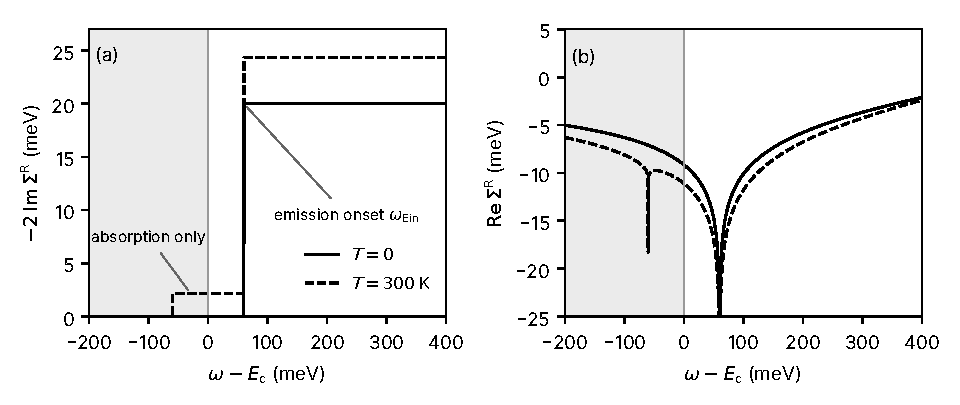
\includegraphics[width=\linewidth]{figures/ch04/fig4_9b.pdf}
  \caption{Self-energy of an electron coupled to a dispersionless boson of energy $\omega_{\mathrm{Ein}} = \SI{60}{meV}$ (\cref{we:4-einstein}), against the energy $\omega$ measured from the bottom $E_{\mathrm{c}}$ of an empty band with a flat density of states over $E_{\mathrm{w}} = \SI{1}{eV}$, for a constant coupling with the golden-rule emission rate $\varGamma_{\mathrm{em}} = \SI{20}{meV}$; solid at $T = 0$, dashed at \SI{300}{K}. The model and its parameters are illustrative. (a) The width $-2\Imag\Sigma^{\mathrm{R}}$: zero below the emission threshold $E_{\mathrm{c}} + \omega_{\mathrm{Ein}}$ at $T = 0$; at \SI{300}{K}, $\varGamma_{\mathrm{em}}n_{\mathrm{B}} = \SI{2.2}{meV}$ from absorption above $E_{\mathrm{c}} - \omega_{\mathrm{Ein}}$, and $\varGamma_{\mathrm{em}}(2n_{\mathrm{B}} + 1)$ where both processes are allowed. (b) The shift $\Real\Sigma^{\mathrm{R}}$, $\SI{-9.14}{meV}$ at $E_{\mathrm{c}}$ for $T = 0$ and $\SI{-11.09}{meV}$ at \SI{300}{K}, with logarithmic singularities at the thresholds caused by the sharp edge of the flat band. Shaded: below the band bottom.}
  \label{fig:4-einstein}
\end{figure}

\subsection{The screened interaction and the \texorpdfstring{$GW$}{GW} self-energy}

The Coulomb version of the same diagram, with a bare line, is the exchange self-energy \cref{eq:D.11-fock}, $\Sigma_{\mathrm{x}}(\vect{k}) = -\Vol^{-1}\sum_{\vect{p}}v_{\mathrm{C}}(|\vect{k} - \vect{p}|)\,n_{\mathrm{F}}(\xi_{\vect{p}})$, the Fock term. It is static, it has no imaginary part, and in a metal it makes the group velocity of the electron gas infinite at the Fermi surface through a logarithm (\cref{app:D.4}). What it misses is screening: while the electron propagates, the other electrons rearrange around it and weaken the interaction at long distances. The rules say how to put this in. Every chain of bubbles that can be inserted into the Coulomb line is a self-energy diagram, and summing the chains replaces the line, exactly as in the random-phase chain:
\begin{equation}
  W^{\mathrm{scr}}(\vect{q},\ii\omega^{\mathrm{B}}_j) = v_{\mathrm{C}}(q) + v_{\mathrm{C}}(q)\,R(\vect{q},\ii\omega^{\mathrm{B}}_j)\,v_{\mathrm{C}}(q) = \varepsilon^{-1}(\vect{q},\ii\omega^{\mathrm{B}}_j)\,v_{\mathrm{C}}(q) .
  \label{eq:4.8-W}
\end{equation}
The last step is \cref{eq:4.4-eps}. With the bubble chain alone, $R$ is the random-phase response \cref{eq:4.8-chain} and $\varepsilon$ the Lindhard function of \cref{sec:4.5} or its crystal form; with the proper blobs it is exact. The screened interaction is the Coulomb potential of a test charge seen through the dielectric response of the target, the same $\varepsilon^{-1}v_{\mathrm{C}}$ that \cref{sec:4.4} found for an external charge, but now at every frequency. In a crystal it is the matrix $W^{\mathrm{scr}}_{\vect{G}\vect{G}'} = (\varepsilon^{-1})_{\vect{G}\vect{G}'}v_{\mathrm{C}}(|\vect{q}+\vect{G}'|)$, and the steps below hold element by element.

Replacing the bare line of the exchange diagram by $W^{\mathrm{scr}}$, and the free propagator by the full one, is the $GW$ approximation of Hedin~\cite{hedin1965new}. In imaginary time,
\begin{equation}
  \Sigma(\vect{k},\ii\omega^{\mathrm{F}}_j) = -\frac1\Vol\sum_{\vect{q}}T\sum_{j'}W^{\mathrm{scr}}(\vect{q},\ii\omega^{\mathrm{B}}_{j'})\,\GF(\vect{k} - \vect{q},\ii\omega^{\mathrm{F}}_j - \ii\omega^{\mathrm{B}}_{j'}) ,
  \label{eq:4.8-GWmats}
\end{equation}
with the convergence factor of rule 5 on the static part $v_{\mathrm{C}}$, which reproduces $\Sigma_{\mathrm{x}}$. At $T = 0$ the real-time rules give the same diagram as
\begin{equation}
  \Sigma(\vect{k},\omega) = \frac{\ii}{\Vol}\sum_{\vect{q}}\int\frac{\dd\omega'}{2\pi}\,\GF(\vect{k} - \vect{q},\omega - \omega')\,W^{\mathrm{scr}}(\vect{q},\omega') ,
  \label{eq:4.8-GW}
\end{equation}
which in space and time is a product, $\Sigma(1,2) = \ii\GF(1,2)W^{\mathrm{scr}}(1,2)$, the form usually written $\Sigma = \ii GW$~\cite[Eqs.~(60) and (61)]{aryasetiawan1998gw}. Note that $\GF$ and $W^{\mathrm{scr}}$ here are time-ordered functions: by the convention of \cref{sec:4.7}, a function without superscript and with a real argument is time-ordered, and $W^{\mathrm{scr}}(\vect{q},\omega')$ equals the retarded $\varepsilon^{-1}v_{\mathrm{C}}$ of \cref{sec:4.4} for $\omega' > 0$ and the advanced one for $\omega' < 0$. Lifetimes need the retarded self-energy, which the Matsubara form \cref{eq:4.8-GWmats} delivers by continuation. The approximation keeps the screening to all orders and drops the vertex corrections, the diagrams in which a further line crosses the one of \cref{fig:4-diagrams}c; Hedin's exact equations contain them in a vertex function, which the $GW$ approximation sets to one~\cite[Eqs.~(43)--(46)]{aryasetiawan1998gw}. With the Hartree term, which is the electrostatic potential of the density, $GW$ is the self-energy behind the quasiparticle gap of silicon in \cref{sec:3.4,sec:4.7}.

The lifetime follows from the same frequency sum as for a boson. The difference $W^{\mathrm{scr}} - v_{\mathrm{C}} = v_{\mathrm{C}}^2R$ is a response function, and like every response it has the spectral representation \cref{eq:4.2-spectral}, $W^{\mathrm{scr}}(\vect{q},z) - v_{\mathrm{C}}(q) = \int\dd\omega'\,B(\vect{q},\omega')/(z - \omega')$, with the weight $B = -\Imag W^{\mathrm{scr},\mathrm{R}}/\pi = v_{\mathrm{C}}(q)L(\vect{q},\omega')/\pi$, where $L$ is the loss function \cref{eq:4.4-SL}. This is a superposition of bosons: the free boson line has $B = |g|^2[\delta(\omega' - \omega_{\vect{Q}}) - \delta(\omega' + \omega_{\vect{Q}})]$, and the screened Coulomb line is a continuum of them, the electron--hole pairs and plasmons of the target, weighted by the loss function. The residue sum that led to \cref{eq:4.8-sigmaboson} then leads, with the free propagator in \cref{eq:4.8-GWmats},
\begin{equation*}
  \Sigma(\vect{k},\ii\omega^{\mathrm{F}}_j) = \Sigma_{\mathrm{x}}(\vect{k}) + \frac1\Vol\sum_{\vect{q}}\int\dd\omega'\,B(\vect{q},\omega')\,\frac{n_{\mathrm{B}}(\omega') + 1 - n_{\mathrm{F}}(\xi_{\vect{k}-\vect{q}})}{\ii\omega^{\mathrm{F}}_j - \xi_{\vect{k}-\vect{q}} - \omega'} ,
\end{equation*}
and the imaginary part of its continuation, $\Imag\Sigma^{\mathrm{R}}(\vect{k},\omega) = -\Vol^{-1}\sum_{\vect{q}}v_{\mathrm{C}}(q)L(\vect{q},\omega')[n_{\mathrm{B}}(\omega') + 1 - n_{\mathrm{F}}(\xi_{\vect{k}-\vect{q}})]$ with $\omega' = \omega - \xi_{\vect{k}-\vect{q}}$. On the shell $\omega = \xi_{\vect{k}}$, with $z_{\mathrm{qp}} \simeq 1$, the width is $\varGamma_{\mathrm{qp}} = -2\Imag\Sigma^{\mathrm{R}}$. The structure-factor relation $2L/v_{\mathrm{C}} = (1 - \ee^{-\beta\omega'})S$ of \cref{eq:4.4-SL}, and the identity $(1 - \ee^{-\beta\omega'})(n_{\mathrm{B}}(\omega') + 1) = 1$, turn it into a rate.
\begin{keyresult}[Electron--electron lifetime in the $GW$ approximation]
\begin{equation}
  \varGamma_{\mathrm{qp}}(\vect{k}) = \int\frac{\dd^3q}{(2\pi)^3}\,v_{\mathrm{C}}(q)^2\,S(\vect{q},\omega')\Bigl[1 - n_{\mathrm{F}}(\xi_{\vect{k}-\vect{q}}) + \ee^{-\beta\omega'}n_{\mathrm{F}}(\xi_{\vect{k}-\vect{q}})\Bigr], \qquad \omega' = \xi_{\vect{k}} - \xi_{\vect{k}-\vect{q}} .
  \label{eq:4.8-lifetime}
\end{equation}
The inverse lifetime of an electron is the rate \cref{eq:4.2-rate} at which it would scatter off the target as a projectile with the potential $\tilde V = v_{\mathrm{C}}$, with the Pauli factor of its final state, plus the rate of the reverse process.
\end{keyresult}
An injected electron is thus a dark-matter particle with a Coulomb coupling. It loses energy to exactly the excitations that the loss function describes, through the same structure factor, and \cref{eq:4.8-lifetime} is a stopping-power calculation of the kind in \cref{eq:4.4-dEdx}, with a quantum recoil and a Pauli-blocked final state. The reverse term, $\ee^{-\beta\omega'}n_{\mathrm{F}}$, is the rate at which electrons in $\vect{k} - \vect{q}$ absorb energy from the target and refill $\vect{k}$, and it is negligible for an electron far above $\mu_{\mathrm{ch}}$. Near the Fermi level of a metal, $1 - n_{\mathrm{F}}$ and the linear low-frequency loss function of \cref{sec:4.5} give the $\xi_{\vect{k}}^2$ of \cref{sec:4.7}. In silicon, $S(\vect{q},\omega')$ vanishes for $\omega'$ below the gap, and an electron cannot decay by creating a pair until it sits at least $\Eg$ above the band edge. Higher up, the loss function peaks at the plasmon near \SI{16.4}{eV} (\cref{sec:4.4}), and an electron with tens of eV loses its energy mostly by plasmon emission. The exchange of the projectile with the electrons it excites, a vertex correction, is absent from \cref{eq:4.8-lifetime}.

In practice the $GW$ quasiparticle energies and lifetimes of silicon are computed in the basis of Kohn--Sham states. The independent-electron response $R^0_{\vect{G}\vect{G}'}$ of \cref{sec:4.6} yields $\varepsilon^{-1}_{\vect{G}\vect{G}'}$ in the random-phase approximation, and \cref{eq:4.8-W} gives the matrix $W^{\mathrm{scr}}_{\vect{G}\vect{G}'}$. The matrix elements $\langle\psi_{n\vect{k}}|\Sigma(\omega)|\psi_{n\vect{k}}\rangle$ of \cref{eq:4.8-GW}, built from the same plane-wave matrix elements, enter the linearized quasiparticle equation \cref{eq:4.7-G0W0}. The frequency integral is the expensive step: a plasmon-pole model, which puts each element of $\Imag\varepsilon^{-1}$ into a single delta function, is accurate for the energies; however, it produces no lifetimes, which need $\Imag\varepsilon^{-1}$ resolved down to the gap.

\subsection{The cutting rule}

The imaginary parts found so far have all been golden-rule rates: the transition sums in \cref{eq:4.7-bubble}, the emission and absorption rates of \cref{we:4-einstein}, the scattering rate \cref{eq:4.8-lifetime}. This is general, and it has a graphical form. After the frequency sums, a diagram at real frequency is a sum of terms, each a product of occupation factors divided by $\omega - E_{\mathrm{cs}} + \ii0^+$, where $E_{\mathrm{cs}}$ is the total energy of a set of lines that together separate the two external points. Its imaginary part replaces each such denominator by $-\pi\delta(\omega - E_{\mathrm{cs}})$, by the Sokhotski--Plemelj formula \cref{eq:2.4-SP}. Drawing a line through the diagram across these propagators, the cut, puts them on shell. The pieces on either side of the cut are the amplitudes to reach the cut state and to return from it, and the imaginary part is $\pi$ times their product summed over the cut states: a golden-rule rate. Cutkosky formulated this rule for relativistic amplitudes~\cite{cutkosky1960singularities}. At finite temperature the occupation factors combine into rates in two ways, and Weldon gave the general form~\cite{weldon1983simple}; we show it for the two diagrams that the book uses.

For the boson self-energy \cref{eq:4.8-sigmaboson}, the cut runs through the electron line and the boson line. Write each thermal factor on its shell as a sum of products of occupations, $n_{\mathrm{B}} + 1 - n_{\mathrm{F}} = (1 + n_{\mathrm{B}})(1 - n_{\mathrm{F}}) + n_{\mathrm{B}}n_{\mathrm{F}}$ and $n_{\mathrm{B}} + n_{\mathrm{F}} = n_{\mathrm{B}}(1 - n_{\mathrm{F}}) + (1 + n_{\mathrm{B}})n_{\mathrm{F}}$. With $\xi' = \xi_{\vect{k}-\vect{Q}}$ and $n_{\mathrm{F}} = n_{\mathrm{F}}(\xi')$,
\begin{equation}
  \begin{gathered}
  -2\Imag\Sigma^{\mathrm{R}}(\vect{k},\omega) = \varGamma_{\mathrm{out}}(\vect{k},\omega) + \varGamma_{\mathrm{in}}(\vect{k},\omega), \\
  \varGamma_{\mathrm{out}} = \frac{2\pi}{\Vol}\sum_{\vect{Q}}|g(\vect{Q})|^2(1 - n_{\mathrm{F}})\Bigl[(1 + n_{\mathrm{B}})\,\delta(\omega - \xi' - \omega_{\vect{Q}}) + n_{\mathrm{B}}\,\delta(\omega - \xi' + \omega_{\vect{Q}})\Bigr], \\
  \varGamma_{\mathrm{in}} = \frac{2\pi}{\Vol}\sum_{\vect{Q}}|g(\vect{Q})|^2\,n_{\mathrm{F}}\Bigl[n_{\mathrm{B}}\,\delta(\omega - \xi' - \omega_{\vect{Q}}) + (1 + n_{\mathrm{B}})\,\delta(\omega - \xi' + \omega_{\vect{Q}})\Bigr] .
  \end{gathered}
  \label{eq:4.8-cutsigma}
\end{equation}
$\varGamma_{\mathrm{out}}$ is the golden-rule rate \cref{eq:2.1-golden} at which an electron in $\vect{k}$ with energy $\omega$ scatters out, by emission or absorption, into an empty state. $\varGamma_{\mathrm{in}}$ is the rate at which electrons scatter into an empty $\vect{k}$ from occupied states. On the shell, $n_{\mathrm{B}}/(1 + n_{\mathrm{B}}) = \ee^{-\beta\omega_{\vect{Q}}}$ and $n_{\mathrm{F}}/(1 - n_{\mathrm{F}}) = \ee^{-\beta\xi'}$, so that $\varGamma_{\mathrm{in}} = \ee^{-\beta\omega}\varGamma_{\mathrm{out}}$, the fermion counterpart of detailed balance. The retarded Green's function is built from an anticommutator, and its width counts the decay of an added electron and the filling of an added hole together. The density response is built from a commutator, and the corresponding combination is a difference.
\begin{keyresult}[Cutting rule]
The imaginary part of the retarded continuation of a diagram is the sum over its cuts, each cut line on shell. For a fermion self-energy, $-2\Imag\Sigma^{\mathrm{R}} = \varGamma_{\mathrm{out}}(1 + \ee^{-\beta\omega})$ with $\varGamma_{\mathrm{out}}$ the golden-rule rate out of the state; for a density response, $-2\Imag R = (1 - \ee^{-\beta\omega})S$ with $S$ the golden-rule sum into the cut states.
\end{keyresult}

\begin{workedexample}{The cut of the bubble}\label{we:4-cut}
The bubble has a single cut, through its two propagators (\cref{fig:4-cut}), and its cut state is one electron--hole pair. With orbitals $\gamma$ in place of plane waves, the density vertex between $\gamma$ and $\gamma'$ is $\langle\gamma'|\ee^{\ii\vect{q}\cdot\vect{r}}|\gamma\rangle$, and the frequency sum \cref{eq:D.10-sum} gives
\begin{equation*}
  R^0(\vect{q},\ii\omega^{\mathrm{B}}_j) = \frac1\Vol\sum_{\gamma\gamma'}\bigl|\langle\gamma'|\ee^{\ii\vect{q}\cdot\vect{r}}|\gamma\rangle\bigr|^2\,\frac{n_\gamma - n_{\gamma'}}{\ii\omega^{\mathrm{B}}_j + E_\gamma - E_{\gamma'}} ,
\end{equation*}
with $n_\gamma = n_{\mathrm{F}}(E_\gamma - \mu_{\mathrm{ch}})$; for plane waves the matrix element is $\delta_{\vect{k}',\vect{k}+\vect{q}}$ and this is \cref{eq:4.7-bubble}. The denominator is $\omega - E_{\mathrm{cs}}$ with $E_{\mathrm{cs}} = E_{\gamma'} - E_\gamma$, the energy of the pair. Continuing to $\omega + \ii0^+$ and cutting,
\begin{equation*}
  -2\Imag R^0(\vect{q},\omega) = \frac{2\pi}{\Vol}\sum_{\gamma\gamma'}\bigl|\langle\gamma'|\ee^{\ii\vect{q}\cdot\vect{r}}|\gamma\rangle\bigr|^2\,(n_\gamma - n_{\gamma'})\,\delta(\omega - E_{\gamma'} + E_\gamma) .
\end{equation*}
The Pauli difference is a difference of two rates. On the shell, $n_{\gamma'}(1 - n_\gamma) = \ee^{-\beta\omega}n_\gamma(1 - n_{\gamma'})$, and $n_\gamma - n_{\gamma'} = n_\gamma(1 - n_{\gamma'}) - n_{\gamma'}(1 - n_\gamma) = (1 - \ee^{-\beta\omega})\,n_\gamma(1 - n_{\gamma'})$: an electron moves from occupied $\gamma$ to empty $\gamma'$, minus the reverse move. The factor $1 - \ee^{-\beta\omega}$ is that of the fluctuation--dissipation theorem \cref{eq:4.2-fdt}, and what it multiplies is
\begin{equation*}
  S^0(\vect{q},\omega) = \frac{2\pi}{\Vol}\sum_{\gamma\gamma'}\bigl|\langle\gamma'|\ee^{\ii\vect{q}\cdot\vect{r}}|\gamma\rangle\bigr|^2\,n_\gamma(1 - n_{\gamma'})\,\delta(\omega - E_{\gamma'} + E_\gamma) ,
\end{equation*}
the golden-rule sum \cref{eq:4.2-S0} over single electron--hole pairs, term by term; for the electron gas at $T = 0$ it is the closed form \cref{eq:4.2-gas}. The terms with $\gamma' = \gamma$ have $n_\gamma - n_{\gamma'} = 0$ and drop out of the bubble; they are the elastic term of \cref{eq:4.2-S0}, which carries no dissipation.
\end{workedexample}

\begin{figure}[tbp]
  \centering
  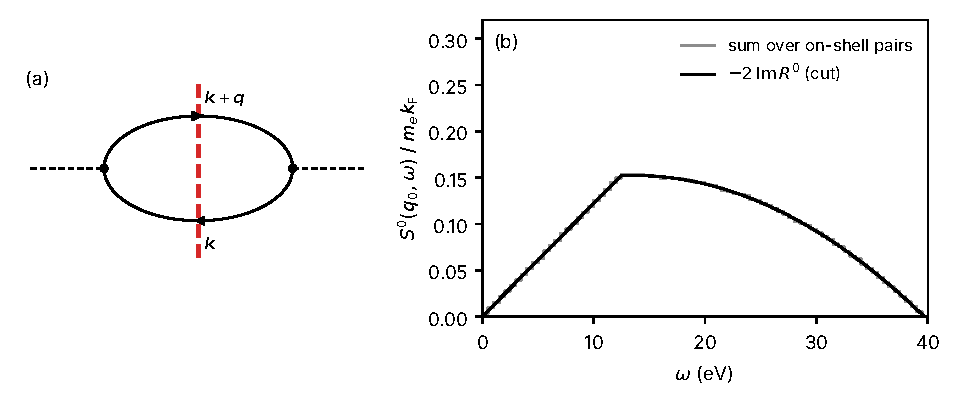
\includegraphics[width=0.45\linewidth]{figures/ch04/fig4_10.pdf}
  \caption{The cut of the bubble. The dashed stubs mark the external momentum $\vect{q}$ at the two density vertices. The cut (dashed vertical line) passes through the electron line $\vect{k}+\vect{q}$ and the hole line $\vect{k}$ and puts both on shell, $\omega = \xi_{\vect{k}+\vect{q}} - \xi_{\vect{k}}$; each half of the diagram is the amplitude for the density operator to create the pair.}
  \label{fig:4-cut}
\end{figure}

Whatever diagram is drawn, its imaginary part counts real final states with positive weights, and every approximation that is a selection of diagrams, with the cuts it allows, has a golden-rule reading. The random-phase chain cuts through electron--hole pairs and plasmons. The ladder, which \cref{sec:4.9} sums, cuts through pairs whose electron and hole are bound into excitons.

\section{Excitons and the Bethe--Salpeter equation}\label{sec:4.9}

The measured absorption spectrum of silicon has a peak of height 36 at \SI{3.42}{eV}, and every approximation of \cref{sec:4.6} leaves only a shoulder of 13 to 15 in its place (\cref{fig:4-si-approx}). The bubble, the local fields and the adiabatic kernel all treat the electron lifted across the gap and the hole it leaves behind as independent. In fact the two carry opposite charges and attract, and the other electrons screen their attraction without cancelling it. In GaAs the attraction binds them into a hydrogen-like state \SI{4.2}{meV} below the gap, which shows up as a sharp line at the absorption edge~\cite{sell1972resolved}, and in silicon the bound pair lies \SI{14.7}{meV} below the indirect gap~\cite{shaklee1970valley}. Such correlated electron--hole pairs, bound or not, are excitons. For dark matter they matter exactly where light particles probe the target: in the first eV above the gap, where the loss function is smallest and the attraction moves spectral weight downward and adds lines below the continuum.

\subsection{The electron--hole Hamiltonian}

In the bubble of \cref{sec:4.8} one density vertex creates a pair, an electron in $(c,\vect{k}+\vect{q})$ and a hole in $(v,\vect{k})$, and the other vertex destroys it; such a pair is a transition, labeled $cv\vect{k}$ at fixed $\vect{q}$. Between the two vertices the pair propagates freely, and in an insulator at $T = 0$ each transition is an eigenstate of the problem with energy $\varepsilon_{c,\vect{k}+\vect{q}} - \varepsilon_{v\vect{k}}$. The ladder of \cref{fig:4-diagrams}(d) lets the electron and the hole interact any number of times on the way, and \cref{app:D.12} sums it with the rules of \cref{app:D.11}. The two first-order insertions of \cref{sec:4.8} become two kernels, and with a statically screened interaction line the sum closes as a matrix equation in the space of transitions, which is an eigenvalue problem.
\begin{keyresult}[Bethe--Salpeter equation in the transition basis]
At momentum transfer $\vect{q}$, the exciton energies $E_\lambda(\vect{q})$ and envelopes $A^\lambda_{cv\vect{k}}(\vect{q})$ solve
\begin{equation}
  \begin{gathered}
  \sum_{c'v'\vect{k}'}H^{\mathrm{exc}}_{cv\vect{k},c'v'\vect{k}'}\,A^\lambda_{c'v'\vect{k}'} = E_\lambda\,A^\lambda_{cv\vect{k}}, \\
  H^{\mathrm{exc}}_{cv\vect{k},c'v'\vect{k}'} = \bigl(\varepsilon_{c,\vect{k}+\vect{q}} - \varepsilon_{v\vect{k}}\bigr)\delta_{cc'}\delta_{vv'}\delta_{\vect{k}\vect{k}'} + g_{\mathrm{deg}}K^{\mathrm{x}}_{cv\vect{k},c'v'\vect{k}'} - K^{\mathrm{d}}_{cv\vect{k},c'v'\vect{k}'} ,
  \end{gathered}
  \label{eq:4.9-bse}
\end{equation}
normalized to $\sum_{cv\vect{k}}|A^\lambda_{cv\vect{k}}|^2 = 1$, with $g_{\mathrm{deg}} = 2$ for the spin singlets that the density creates. The exchange and direct kernels are
\begin{equation}
  \begin{aligned}
  K^{\mathrm{x}}_{cv\vect{k},c'v'\vect{k}'} &= \frac1\Vol\sum_{\vect{G}\ne0}v_{\mathrm{C}}(|\vect{q}+\vect{G}|)\,\rho_{cv}(\vect{k},\vect{q}+\vect{G})\,\rho_{c'v'}(\vect{k}',\vect{q}+\vect{G})^* ,\\
  K^{\mathrm{d}}_{cv\vect{k},c'v'\vect{k}'} &= \frac1\Vol\sum_{\vect{G}\vect{G}'}\rho_{cc'}(\vect{k}'+\vect{q},\vect{p}+\vect{G})\,W^{\mathrm{scr}}_{\vect{G}\vect{G}'}(\vect{p},\omega = 0)\,\rho_{vv'}(\vect{k}',\vect{p}+\vect{G}')^*, \quad \vect{p} = \vect{k} - \vect{k}' ,
  \end{aligned}
  \label{eq:4.9-kernels}
\end{equation}
with the density vertices of \cref{eq:3.2-rho}, the screened interaction $W^{\mathrm{scr}}_{\vect{G}\vect{G}'} = (\varepsilon^{-1})_{\vect{G}\vect{G}'}v_{\mathrm{C}}(|\vect{p}+\vect{G}'|)$ of \cref{eq:4.8-W}, and quasiparticle band energies.
\end{keyresult}
\Cref{eq:4.9-bse} is \cref{eq:E.6-Hexc} at finite $\vect{q}$. The exchange kernel is the one of \cref{sec:4.6,sec:4.8}, the Coulomb interaction without its $\vect{G} = 0$ term. For a momentum transfer beyond the first zone, $\vect{q} = \vect{q}_r + \vect{G}_q$ in the unreduced indexing of \cref{sec:4.4}, the kernels are written with $\vect{q}_r$ in place of $\vect{q}$, and the omitted term of $K^{\mathrm{x}}$ is then the one at $\vect{G} = \vect{G}_q$.

Each piece of $H^{\mathrm{exc}}$ has a plain meaning. The diagonal is the energy of the free pair. It must be a quasiparticle energy (\cref{sec:4.7}), because the self-energy insertions of the ladder are summed into the propagators, and with Kohn--Sham bands a scissor (\cref{eq:3.4-scissor}) takes their place. The direct kernel is the Coulomb interaction between the electron and the hole, screened by all the other electrons. The electron scatters from $(c,\vect{k}+\vect{q})$ to $(c',\vect{k}'+\vect{q})$ and the hole from $(v,\vect{k})$ to $(v',\vect{k}')$, so the pair keeps its total momentum $\vect{q}$ and its constituents exchange $\vect{p}$. Its diagonal element is the Coulomb energy of two positive densities, $|\psi_{c,\vect{k}+\vect{q}}|^2$ and $|\psi_{v\vect{k}}|^2$. Since that energy is positive, $-K^{\mathrm{d}}$ lowers the pair energy: it is the attraction. At large separation the screened interaction of two charges in an insulator is $e^2/(4\pi\varepsilon_\infty r)$, and this long-range tail is what binds the pairs of the next subsection. The exchange kernel describes something else. The pair annihilates at one point and a pair is re-created at another, and the Coulomb line between them is the microscopic Hartree potential of the induced density. It is the local-field kernel of \cref{sec:4.6}, positive on the diagonal and repulsive. The long-range term $\vect{G} = 0$ is left out because it is the macroscopic field, which the definition of $\varepsilon_{\mathrm{mac}}$ already treats on its own (\cref{eq:D.12-epsmac}); added back, it yields the full density response (\cref{app:D.12}). Exchange is also what distinguishes the spin states. The density vertex couples to both spins alike, so $K^{\mathrm{x}}$ couples a transition of either spin to one of either spin and appears with $g_{\mathrm{deg}}$ in the singlet, while the triplet feels only $-K^{\mathrm{d}}$ and is not excited by a density coupling at all.

Behind \cref{eq:4.9-bse} stand a kernel without the change of the screening, a static screened interaction and the Tamm--Dancoff approximation, and \cref{app:D.12} makes each one explicit. The kernel is the change of the Hartree potential plus the $GW$ self-energy of \cref{sec:4.8} when the Green's function changes, with the change of $W^{\mathrm{scr}}$ itself neglected~\cite{hanke1980many,strinati1988application}. The screened interaction is static: $W^{\mathrm{scr}}$ is taken at zero frequency, which is good when the binding energies and the spread of transition energies that matter are small against the frequencies at which $\varepsilon^{-1}$ changes, set in silicon by the plasma frequency of \SI{16.6}{eV}. What is lost is the retarded response of the other electrons to the moving pair. And the coupling between the creation and the annihilation of a pair is dropped, the Tamm--Dancoff approximation, whose error on $E_\lambda$ is of second order in the kernel divided by twice the gap. With these choices $H^{\mathrm{exc}}$ is Hermitian (\cref{app:D.12}), and its eigenvectors are orthonormal.

Without kernels each transition is its own eigenstate and the response is the bubble of \cref{eq:4.6-R0}. With $K^{\mathrm{d}}$ switched off, $H^{\mathrm{exc}} = \mathbf{D} + g_{\mathrm{deg}}\mathbf{X}\mathbf{X}^\dagger$, where $\mathbf{D}$ is the diagonal matrix of transition energies and the column of $\mathbf{X}$ for each $\vect{G}\ne0$ holds the vertices $\rho_{cv}(\vect{k},\vect{q}+\vect{G})$ times $[v_{\mathrm{C}}(|\vect{q}+\vect{G}|)/\Vol]^{1/2}$. Projected on the vertices, the resolvent $(\omega - H^{\mathrm{exc}})^{-1}$ becomes, by the Woodbury identity \cref{eq:C.7-woodbury},
\begin{equation*}
  \mathbf{X}^\dagger\bigl(\omega - \mathbf{D} - g_{\mathrm{deg}}\mathbf{X}\mathbf{X}^\dagger\bigr)^{-1}\mathbf{X} = \mathbf{M}\bigl(\mathbf{1} - g_{\mathrm{deg}}\mathbf{M}\bigr)^{-1}, \qquad \mathbf{M} = \mathbf{X}^\dagger(\omega - \mathbf{D})^{-1}\mathbf{X} .
\end{equation*}
Here $g_{\mathrm{deg}}\mathbf{M}$ is the resonant part of $R^0$ of \cref{eq:4.6-R0} between the vertices at $\vect{G} \ne 0$, sandwiched between factors $\bar v^{1/2}$, and $g_{\mathrm{deg}}\mathbf{M}(\mathbf{1} - g_{\mathrm{deg}}\mathbf{M})^{-1}$, with the same factors, is the geometric series of $\bar R = R^0 + R^0\bar v\bar R$ on the block $\vect{G},\vect{G}' \ne 0$; the head $\bar R_{\vect{0}\vect{0}}$ follows from the same equation with the row $\vect{G} = 0$ of $R^0$, which is \cref{eq:4.6-rpaLF}. The random-phase approximation with local fields is thus the Bethe--Salpeter equation without the attraction, as \cref{sec:4.6} anticipated.

In practice the equation is set up from the same states as the random-phase response, with the screened interaction $\varepsilon^{-1}_{\vect{G}\vect{G}'}(\vect{p})$ computed beforehand for every difference $\vect{p}$ of two grid points. Its dimension is the number of transitions, $N_vN_cN_k$, and the $\vect{k}$ grid sets the cost: the kernel has $(N_vN_cN_k)^2$ elements, and a converged spectrum of silicon needs several thousand points in the zone. The spectrum then comes from an iterative (Lanczos--Haydock) solver, which needs products of $H^{\mathrm{exc}}$ with a vector and nothing else, and a full diagonalization is needed when individual envelopes are wanted.

\subsection{Wannier--Mott excitons}

When the attraction is weak, the pair it binds is large, and a large pair samples just the bands near their extrema and the screening at long wavelengths. \Cref{eq:4.9-bse} then reduces to the hydrogen atom, a result of Wannier and of Mott~\cite{wannier1937structure,mott1938conduction}. Take a direct gap at $\vect{k} = 0$, as in GaAs, with one isotropic conduction band of mass $m^*$, one valence band of hole mass $m_{\mathrm{h}}$, and $\vect{q} \to 0$. Near the extrema the transition energy is
\begin{equation*}
  \varepsilon_{c\vect{k}} - \varepsilon_{v\vect{k}} = \Eg + \frac{k^2}{2m^*} + \frac{k^2}{2m_{\mathrm{h}}} = \Eg + \frac{k^2}{2\mu_x}, \qquad \frac{1}{\mu_x} = \frac{1}{m^*} + \frac{1}{m_{\mathrm{h}}} ,
\end{equation*}
with $\mu_x$ the reduced mass of the exciton. Suppose the envelope $A_{\vect{k}}$ is confined to $|\vect{k}|$ small against the zone; we check this at the end. Then $\vect{p} = \vect{k} - \vect{k}'$ is small too, and in the direct kernel only $\vect{G} = \vect{G}' = 0$ survives: the terms with $\vect{G} \ne 0$ carry vertices between nearly equal states at momentum transfer $|\vect{p} + \vect{G}| \approx |\vect{G}|$, which are small, and a Coulomb factor that is finite instead of singular. The two vertices at $\vect{G} = 0$ are overlaps of the periodic parts of the same band at nearby $\vect{k}$, $\rho_{cc}(\vect{k},\vect{p}) \simeq \rho_{vv}(\vect{k},\vect{p}) \simeq 1$ (\cref{eq:3.2-rho}), and the screened interaction at small $\vect{p}$ is the bare one divided by $\varepsilon_\infty$. The direct kernel becomes
\begin{equation*}
  K^{\mathrm{d}}_{\vect{k}\vect{k}'} \simeq \frac{1}{\Vol}\,\frac{e^2}{\varepsilon_\infty|\vect{k} - \vect{k}'|^2} .
\end{equation*}
The exchange kernel, without its $\vect{G} = 0$ term, is however short-ranged in the relative coordinate: it acts only when the electron and the hole sit in the same cell. For a pair spread over many cells its effect is smaller than that of $K^{\mathrm{d}}$ by the probability of finding the two in one cell, and we drop it. It splits the singlet from the triplet by a small amount, the electron--hole exchange splitting. \Cref{eq:4.9-bse} now reads
\begin{equation*}
  \Bigl(\Eg + \frac{k^2}{2\mu_x}\Bigr)A_{\vect{k}} - \frac1\Vol\sum_{\vect{k}'}\frac{e^2}{\varepsilon_\infty|\vect{k} - \vect{k}'|^2}\,A_{\vect{k}'} = E\,A_{\vect{k}} .
\end{equation*}
Define the envelope function $F(\vect{r}) = \Vol^{-1/2}\sum_{\vect{k}}A_{\vect{k}}\ee^{\ii\vect{k}\cdot\vect{r}}$, the Fourier transform of the envelope in the relative coordinate $\vect{r}$ of the electron and the hole; by Parseval, $\int\dd^3r\,|F|^2 = \sum_{\vect{k}}|A_{\vect{k}}|^2 = 1$. Multiplying by $\Vol^{-1/2}\ee^{\ii\vect{k}\cdot\vect{r}}$ and summing over $\vect{k}$ turns $k^2$ into $-\nabla^2$, and the kernel, a convolution in $\vect{k}$, into a product in $\vect{r}$ with the transform of $e^2/(\varepsilon_\infty k^2)$, which is $e^2/(4\pi\varepsilon_\infty r)$ by \cref{eq:A.2-vC}. The result is a Schr\"odinger equation for the relative motion,
\begin{equation}
  \Bigl[-\frac{\nabla^2}{2\mu_x} - \frac{\alpha}{\varepsilon_\infty r}\Bigr]F(\vect{r}) = (E - \Eg)\,F(\vect{r}) ,
  \label{eq:4.9-envelope}
\end{equation}
the hydrogen atom with $m_e \to \mu_x$ and $\alpha \to \alpha/\varepsilon_\infty$. Its bound states follow from those of hydrogen by the same substitution.
\begin{keyresult}[Wannier--Mott excitons]
Below the gap the pair has the levels $E_n = \Eg - E_x^b/n^2$, $n = 1, 2, \dots$, with the binding energy and radius
\begin{equation}
  E_x^b = \frac{\mu_x\alpha^2}{2\varepsilon_\infty^2} = \frac{\mu_x}{m_e}\,\frac{\SI{13.61}{eV}}{\varepsilon_\infty^2}, \qquad
  a_x = \frac{\varepsilon_\infty}{\alpha\mu_x} = \varepsilon_\infty\,\frac{m_e}{\mu_x}\,a_0 ,
  \label{eq:4.9-WM}
\end{equation}
and hydrogenic envelopes; the ground state is $F_{1s}(\vect{r}) = \ee^{-r/a_x}/(\pi a_x^3)^{1/2}$, and $|F_{ns}(0)|^2 = 1/(\pi a_x^3n^3)$. Above $\Eg$ the unbound solutions form the continuum of scattering states.
\end{keyresult}
The approximation holds when the exciton is large compared with the lattice constant, $a_x \gg a$. Then the envelope occupies a region of size $1/a_x$ around the band extremum, where the bands are parabolic and the vertices close to one, and the electron and the hole are far enough apart for the macroscopic $\varepsilon_\infty$ to screen them. Static screening needs a second condition: the internal motion of the pair, at frequencies $\sim E_x^b$, must be slow against the response that screens it. For the electrons, which respond at energies of the gap and above, this is the case whenever $E_x^b \ll \Eg$. The lattice of a polar crystal also screens, with the ions responding at the optical-phonon energies. If $E_x^b$ is small against these, the ions follow the pair, and the static constant $\varepsilon_0$ with the lattice included (\cref{sec:5.5}) takes the place of $\varepsilon_\infty$; if it is large, the ions cannot follow and $\varepsilon_\infty$ is right. In between, the interaction is not of the form $1/r$ at all.

In silicon the pair is indirect. Its lowest state has the electron in one of the conduction valleys near $\vect{k}_{\mathrm{c}}$ and the hole at the valence maximum at $\mathrm{\Gamma}$, and its total crystal momentum is $\vect{k}_{\mathrm{c}}$ (\cref{sec:3.3}). The relative motion is still governed by \cref{eq:4.9-envelope}, now with the anisotropic valley mass and the degenerate, warped valence band. A spherical estimate brackets it. The kinetic energy of an $s$ state averaged over directions involves $(1/3)(1/m^*_\parallel + 2/m^*_\perp)$, an electron mass of $0.26\,m_e$ from the masses of \cref{tab:3-materials}; with the heavy-hole mass between its values along [100] and [111], 0.28 and $0.72\,m_e$, \cref{eq:4.9-WM} with $\varepsilon_\infty = 11.7$ gives 13 to \SI{19}{meV}. The measured binding is \SI{14.7}{meV}~\cite{shaklee1970valley}. Read through \cref{eq:4.9-WM}, it corresponds to $\mu_x = 0.148\,m_e$ and to a radius $a_x = \SI{4.2}{nm}$, nearly eight lattice constants, and the large-exciton picture holds. In crystal momentum the envelope has a width $1/a_x = \SI{0.024}{\angstrom^{-1}}$, about one percent of the zone, $|\vect{G}_{111}| = \SI{2.0}{\angstrom^{-1}}$. A calculation of this state with \cref{eq:4.9-bse} on a uniform grid would need hundreds of points per direction, which is why bound excitons near the gap are computed with grids refined around the band extrema, or in the effective-mass limit itself. Since silicon is not polar, $\varepsilon_0 = \varepsilon_\infty$ and the question of the lattice does not arise.

\begin{workedexample}{The Wannier--Mott exciton of GaAs}\label{we:4-gaasexciton}
The conduction band of GaAs at $\mathrm{\Gamma}$ has $m^* = 0.067\,m_e$, and the valence maximum is the fourfold level of heavy and light holes (\cref{tab:3-materials}). For a hydrogenic estimate the hole needs one mass. The two hole energies of \cref{eq:3.3-holes} at the same $\vect{\kappa}$ differ by the sign of the square root, so their mean is $\gamma^{\mathrm{Lu}}_1\kappa^2/2m_e$ in every direction: averaged over the two branches, the hole moves with the inverse mass $\gamma^{\mathrm{Lu}}_1/m_e$. With $\gamma^{\mathrm{Lu}}_1 = 6.98$,
\begin{equation*}
  \frac{m_e}{\mu_x} = \frac{1}{0.067} + 6.98 = 21.9, \qquad \mu_x = 0.0457\,m_e .
\end{equation*}
With the measured electronic constant $\varepsilon_\infty = 10.88$~\cite{lockwood2005optical}, \cref{eq:4.9-WM} gives
\begin{equation*}
  E_x^b = 0.0457\times\frac{\SI{13.61}{eV}}{10.88^2} = \SI{5.25}{meV}, \qquad a_x = 10.88\times\frac{\SI{0.529}{\angstrom}}{0.0457} = \SI{12.6}{nm} ,
\end{equation*}
22 lattice constants, which keeps the envelope well inside the parabolic region. The measured binding energy is \SI{4.2}{meV}~\cite{sell1972resolved}, and the estimate with $\varepsilon_\infty$ overbinds by a quarter. The reason is the lattice. The optical phonons of GaAs lie near \SI{35}{meV}~\cite[Fig.~2]{griffin2018directional}, eight times the binding energy, so the ions follow the slow relative motion of the pair and add their own screening. With the static constant $\varepsilon_0 = 12.9$~\cite[Table~I]{griffin2018directional}, the binding falls to $0.0457\times\SI{13.61}{eV}/12.9^2 = \SI{3.74}{meV}$ and the radius grows to \SI{14.9}{nm}. Most of the remaining difference from the measurement, \SI{0.5}{meV}, comes from the part of the hole kinetic energy that the average over the two branches throws away. That part mixes heavy and light holes, has no first-order effect on the $1s$ state by symmetry, and lowers its energy in second order~\cite{baldereschi1971energy}. Either way the binding is a few meV, small against the gap of \SI{1.52}{eV}, and the exciton is a line just below the absorption edge. \Cref{sec:5.5} derives $\varepsilon_0$ and the lattice contribution to the screening.
\end{workedexample}

At finite momentum transfer the pair moves as a whole. Take the transitions from $(v,\vect{k})$ to $(c,\vect{k}+\vect{q})$ with a conduction minimum at $\vect{k}_{\mathrm{c}}$ (zero for GaAs) and $\vect{Q} = \vect{q} - \vect{k}_{\mathrm{c}}$, small. The transition energy is $\Eg + (\vect{k} + \vect{Q})^2/2m^* + k^2/2m_{\mathrm{h}}$. With $\vect{k} = \vect{\kappa} - m_{\mathrm{h}}\vect{Q}/(m^* + m_{\mathrm{h}})$, the terms linear in $\vect{\kappa}$ cancel and it becomes $\Eg + Q^2/[2(m^* + m_{\mathrm{h}})] + \kappa^2/2\mu_x$. Since the direct kernel depends only on $\vect{k} - \vect{k}' = \vect{\kappa} - \vect{\kappa}'$, the relative motion obeys \cref{eq:4.9-envelope} unchanged, and
\begin{equation}
  E_n(\vect{q}) = \Eg - \frac{E_x^b}{n^2} + \frac{(\vect{q} - \vect{k}_{\mathrm{c}})^2}{2(m^* + m_{\mathrm{h}})} .
  \label{eq:4.9-dispersion}
\end{equation}
The exciton has the center-of-mass dispersion of a particle with the total mass of the pair, the same mass that governs the pair threshold $E_{\mathrm{min}}(\vect{q})$ near a valley in \cref{eq:3.3-Eminpar}. The bound levels follow the threshold, $E_{x}^b/n^2$ below it. In silicon the lowest exciton sits at $\vect{q} \simeq \vect{k}_{\mathrm{c}}$, \SI{14.7}{meV} below the indirect gap, at a crystal momentum that a photon cannot supply. Light reaches it only with a phonon (\cref{sec:6.5}), while dark matter that transfers $\vect{q} \approx \vect{k}_{\mathrm{c}}$ can create it on its own.

\subsection{Excitonic absorption and scattering}

The eigenpairs of \cref{eq:4.9-bse} give the macroscopic dielectric function directly. In the resonant block the resolvent of the pair is $(\omega - H^{\mathrm{exc}} + \ii0^+)^{-1} = \sum_\lambda A^\lambda A^{\lambda\dagger}/(\omega - E_\lambda + \ii0^+)$, and projecting it on the density vertices at $\vect{q}$, as in \cref{eq:D.12-Rexc}, gives the response $\bar R_{\vect{0}\vect{0}}$ that is proper with respect to the long-range Coulomb term. With \cref{eq:4.6-rpaLF}, $\varepsilon_{\mathrm{mac}} = 1 - v_{\mathrm{C}}(q)\bar R_{\vect{0}\vect{0}}$,
\begin{equation}
  \varepsilon_{\mathrm{mac}}(\vect{q},\omega) = 1 - \frac{g_{\mathrm{deg}}e^2}{Vq^2}\sum_\lambda\Bigl|\sum_{cv\vect{k}}A^\lambda_{cv\vect{k}}\,\rho_{cv}(\vect{k},\vect{q})^*\Bigr|^2
  \left[\frac{1}{\omega - E_\lambda + \ii0^+} - \frac{1}{\omega + E_\lambda + \ii0^+}\right] ,
  \label{eq:4.9-epsmac}
\end{equation}
where the antiresonant term, with its poles at $-E_\lambda$, is the mirror image that the Tamm--Dancoff approximation keeps. Its imaginary part at $\omega > 0$ and its static limit are
\begin{equation}
  \begin{gathered}
  \varepsilon_2(\vect{q},\omega) = \frac{\pi g_{\mathrm{deg}}e^2}{Vq^2}\sum_\lambda\Bigl|\sum_{cv\vect{k}}A^\lambda_{cv\vect{k}}\,\rho_{cv}(\vect{k},\vect{q})^*\Bigr|^2\delta(\omega - E_\lambda), \\
  \varepsilon_{\mathrm{mac}}(\vect{q},0) = 1 + \frac{2g_{\mathrm{deg}}e^2}{Vq^2}\sum_\lambda\frac{\bigl|\sum_{cv\vect{k}}A^\lambda_{cv\vect{k}}\rho_{cv}(\vect{k},\vect{q})^*\bigr|^2}{E_\lambda} .
  \end{gathered}
  \label{eq:4.9-eps2}
\end{equation}
At $\vect{q} \to 0$ the vertex is the optical one, $\rho_{cv} = \vect{q}\cdot\vect{v}_{cv}/(\varepsilon_{c\vect{k}} - \varepsilon_{v\vect{k}})$ (\cref{eq:3.2-optical}), the factor $q^2$ cancels, and the static limit is the constant $\varepsilon_\infty$. Without kernels each $\lambda$ is a single transition, and the two reduce to \cref{eq:4.6-eps2,eq:4.6-static}.

The new object is the exciton oscillator strength, the squared modulus of a coherent sum. Independent transitions contribute $|\rho_{cv}|^2$ each, whatever their phases. An exciton, however, contributes the square of the sum of the amplitudes of the transitions it is made of, weighted by $A^\lambda$. When the attraction lowers a state, the transitions in it add in phase, the low-lying excitons collect the oscillator strength of many transitions, and the weight moves to lower energy. Through the static limit in \cref{eq:4.9-eps2}, with $E_\lambda$ in the denominator, this also raises $\varepsilon_\infty$. The f-sum rule of \cref{sec:4.3} fixes the total weight of the exact response, so the weight gained at low energies is lost higher up.

For a Wannier--Mott exciton the coherent sum has a closed form. The vertex varies little across the region of size $1/a_x$ that the envelope occupies, and with $\sum_{\vect{k}}A^\lambda_{\vect{k}} = \Vol^{1/2}F_\lambda(0)$, from the definition of $F$,
\begin{equation}
  \Bigl|\sum_{cv\vect{k}}A^\lambda_{cv\vect{k}}\,\rho_{cv}(\vect{k},\vect{q})^*\Bigr|^2 \simeq \Vol\,|F_\lambda(0)|^2\,|\rho_{cv}(\vect{k}_0,\vect{q})|^2 ,
  \label{eq:4.9-elliott}
\end{equation}
with $\vect{k}_0$ the valence extremum. Only $s$ states, whose envelope does not vanish where the electron and the hole coincide, are excited. Their strengths fall as $|F_{ns}(0)|^2 = 1/(\pi a_x^3n^3)$, and since the levels crowd toward the gap as $n^{-2}$, the weight per unit energy just below $\Eg$ joins smoothly onto that of the continuum above it. The continuum itself is enhanced over the independent-particle one near the edge, since the attraction raises the probability of finding the electron at the hole. Both results are Elliott's~\cite{elliott1957intensity}. Compared with independent particles, whose absorption at a direct edge rises from zero as $(\omega - \Eg)^{1/2}$, the excitonic edge starts with a series of lines and a finite step.

\Cref{fig:4-bse} shows what the attraction does to silicon at $\vect{q} \to 0$, in a model calculation with the empirical pseudopotential states of \cref{sec:3.3}. One property of these states decides how the figure is read. The bands were fitted to the measured positions of the absorption peaks, and those positions already contain the downward shift that the electron--hole attraction produces. Adding the attraction on top of the fitted bands counts that shift a second time, and every peak of the model lands too low. The figure therefore tests what the attraction does to the shape and the weight of the spectrum, not where the peaks lie. All three spectra come from one Hamiltonian, \cref{eq:4.9-bse}, on the same transitions: without kernels, with $g_{\mathrm{deg}}K^{\mathrm{x}}$ alone, and with $g_{\mathrm{deg}}K^{\mathrm{x}} - K^{\mathrm{d}}$. The screened interaction in $K^{\mathrm{d}}$ is the model's own random-phase one with local fields. On this grid the diagonal elements of $K^{\mathrm{d}}$ average \SI{81}{meV}, a measure of the attraction between an electron and a hole spread over the crystal. The number depends on the grid, since the term at $\vect{p} \to 0$ grows with the volume of the zone per $\vect{k}$ point. The full random-phase result with local fields, computed from \cref{eq:4.6-rpaLF} on the same states without the Tamm--Dancoff approximation, differs from the spectrum with $K^{\mathrm{x}}$ alone by 3.4 percent of the peak, which is the Tamm--Dancoff error here.

\begin{figure}[tbp]
  \centering
  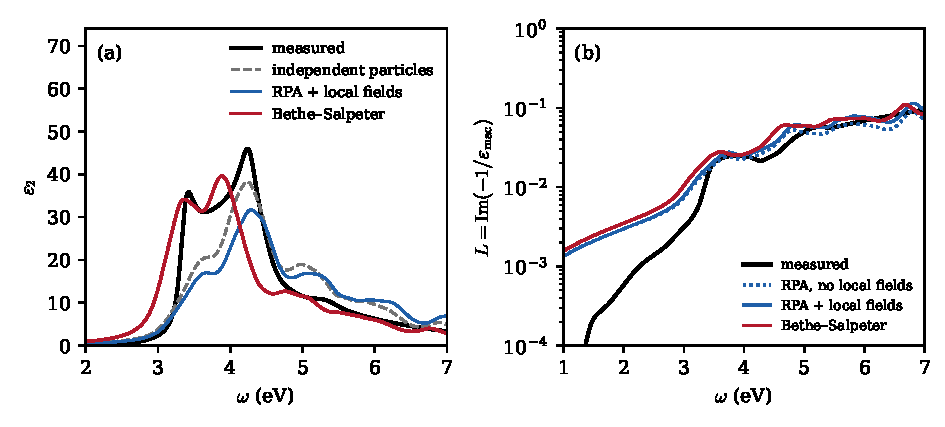
\includegraphics[width=\linewidth]{figures/ch04/fig4_11.pdf}
  \caption{The electron--hole attraction in the optical spectrum of crystalline silicon at $\vect{q} \to 0$, in a model calculation. Band energies and states come from the local empirical pseudopotential of Cohen and Bergstresser~\cite{cohen1966band}, fitted to measured transition energies, as in \cref{fig:4-si-approx}. All curves come from the transition-basis Hamiltonian \cref{eq:4.9-bse} in the Tamm--Dancoff approximation. The basis has 4 valence and 3 conduction bands on a shifted $12^3$ grid of $\vect{k}$ points over the full zone (20{,}736 transitions); both kernels use the 59 shortest reciprocal vectors, and the spectra carry a Lorentzian broadening of \SI{0.15}{eV}. The direct kernel uses the diagonal of the model's static inverse dielectric matrix in the random-phase approximation with local fields, computed with 26 conduction bands; spectra by the Lanczos--Haydock method. Black: measured at \SI{300}{K}~\cite{franta2017temperature}. (a) $\varepsilon_2$: independent particles (dashed gray), the random-phase approximation with local fields, that is, exchange kernel only (blue), and the Bethe--Salpeter equation with both kernels (red). The attraction turns the shoulder near \SI{3.4}{eV} into a peak; the whole spectrum shifts down because the fitted bands already contain part of the excitonic shift. (b) Loss function $L$ on a logarithmic scale for the same three cases (dotted blue: no local fields, which has the independent-particle $\varepsilon_2$). Below about \SI{3}{eV} the model curves are the Lorentzian tails of transitions that start at \SI{3.13}{eV} on this grid, and lie above the measured $L$, which has no such tails.}
  \label{fig:4-bse}
\end{figure}

The attraction restores the lower peak. At \SI{3.42}{eV} independent particles give 15 and local fields 13; with the direct kernel the spectrum has a peak of height 34 at \SI{3.36}{eV}, against the measured 36 at \SI{3.42}{eV}. This peak, however, is not a bound state. The vertical transitions of silicon start near \SI{3.1}{eV}, and the strength comes from many transitions along a region of the zone where conduction and valence bands run nearly parallel, which the attraction mixes coherently. The upper peak moves down to \SI{3.88}{eV}, \SI{0.36}{eV} below the measured \SI{4.24}{eV}, which is the double counting described above. First-principles calculations avoid it by starting from quasiparticle energies of a $GW$ calculation, which contain no excitonic shift. The Bethe--Salpeter spectrum of silicon computed that way by Albrecht and coworkers places both main peaks at the measured energies with the measured ratio of their heights, and overestimates their absolute heights slightly~\cite{albrecht1998ab}. In the model, the static constant rises by 17 percent over the random-phase value with local fields in the same basis of bands. Part of that rise is again the double counting, since $\varepsilon_\infty$ weights each exciton by $1/E_\lambda$, and the ratio is an upper estimate of what the attraction adds to the local-field value of \cref{we:4-siepsinf}.

For dark matter the loss function in panel (b) is the relevant quantity. At \SI{3}{eV} the attraction raises $L$ by 36 percent over the random-phase value with local fields; from 4 to \SI{6}{eV} the two agree within 3.5 percent. The effect is concentrated in the first eV of the absorption, exactly where a slow particle deposits its energy.

At finite $\vect{q}$ the dark-matter rate needs the structure factor rather than $\varepsilon_2$. At $T = 0$ and $\omega > 0$, \cref{eq:4.4-SL} gives $S = (2q^2/e^2)L$, with $L = \Imag(-1/\varepsilon_{\mathrm{mac}}) = \varepsilon_2/|\varepsilon_{\mathrm{mac}}|^2$, and \cref{eq:4.9-eps2} then yields the exciton contribution
\begin{equation}
  S(\vect{q},\omega) = \frac{2\pi g_{\mathrm{deg}}}{\Vol}\sum_\lambda\frac{\bigl|\sum_{cv\vect{k}}A^\lambda_{cv\vect{k}}(\vect{q})\,\rho_{cv}(\vect{k},\vect{q})^*\bigr|^2}{|\varepsilon_{\mathrm{mac}}(\vect{q},\omega)|^2}\,\delta\bigl(\omega - E_\lambda(\vect{q})\bigr) .
  \label{eq:4.9-S}
\end{equation}
Each exciton is a line at $E_\lambda(\vect{q})$ whose weight is its oscillator strength, screened by the factor $1/|\varepsilon_{\mathrm{mac}}|^2$ of \cref{sec:4.4}. The exact statement is $S = (2q^2/e^2)\varepsilon_2/|\varepsilon_{\mathrm{mac}}|^2$, and the line form holds when the line's own contribution to $\varepsilon_{\mathrm{mac}}$ near its energy is small against the background, whose value then goes into the denominator. A line strong enough to change $\varepsilon_{\mathrm{mac}}$ near its own energy is moved up by the long-range exchange energy, since the pole of $L$ sits at the zero of $\varepsilon_{\mathrm{mac}}$. This is the electronic analog of the splitting between the longitudinal optical (LO) and transverse optical (TO) phonons of a polar crystal, in which the macroscopic field of a longitudinal lattice vibration raises its frequency above that of the transverse one (\cref{sec:5.5}). With the $\vect{G} = 0$ term kept in the kernel, the eigenvalues are these shifted energies and the weights are not divided by $|\varepsilon_{\mathrm{mac}}|^2$ (\cref{eq:D.12-S}). At the momentum transfers of a few keV that dark matter typically deposits, the Coulomb factor $e^2/q^2$ is small and the shift is negligible. Without kernels, \cref{eq:4.9-S} is the independent-particle structure factor \cref{eq:4.2-S0} screened by $1/|\varepsilon_{\mathrm{mac}}|^2$, the random-phase result for the electrons.

For a Wannier--Mott exciton, \cref{eq:4.9-elliott} and \cref{eq:4.9-dispersion} make the lines explicit,
\begin{equation*}
  S(\vect{q},\omega) = 2\pi g_{\mathrm{deg}}\,\frac{|\rho_{cv}(\vect{k}_0,\vect{q})|^2}{|\varepsilon_{\mathrm{mac}}(\vect{q},\omega)|^2}\sum_n\frac{1}{\pi a_x^3n^3}\,\delta\bigl(\omega - E_n(\vect{q})\bigr) ,
\end{equation*}
a weight per unit volume set by the probability $|F_{ns}(0)|^2$ of finding the electron at the hole, times the squared vertex between the two band extrema. In silicon the lowest line follows the indirect threshold of \cref{sec:3.3} at $\vect{q} \approx \vect{k}_{\mathrm{c}}$ and lies \SI{14.7}{meV} below it. As a shift of the threshold this is 1.3 percent of the gap, small for the threshold mass of \cref{sec:3.3}. As a redistribution of weight, however, it matters more: the edge of the zero-phonon response starts with a line, and the continuum above it is enhanced. Light dark matter samples exactly this region, and \cref{sec:10.5} computes the excitonic loss function at finite $\vect{q}$.

\subsection{Levels of approximation}

Each approximation contains the previous one as a limit: $K^{\mathrm{d}} \to 0$ gives local fields, $\bar v \to 0$ the random-phase head, and the head alone at fixed energies the independent particles. What the Bethe--Salpeter equation in this form leaves out are the dynamical screening of the interaction, the coupling of pair creation and annihilation, and every process with a phonon, which \cref{chap:6} adds.

In silicon the approximations of \cref{fig:4-si-approx,fig:4-bse} differ in characteristic ways. The static constant falls with the local fields and rises part of the way back with the adiabatic kernel (\cref{we:4-siepsinf}), and in the model the attraction raises it by 17 percent above the local-field value of 10.22, to about 11.9. The screening factor $1/\varepsilon_\infty^2$ at small $q$ thus varies by up to a third across the hierarchy. At the lower absorption peak the spread is a factor of more than two, 13 to 34, and the loss function at \SI{3}{eV} changes by a third between the adiabatic kernel and the Bethe--Salpeter equation alone. Above about \SI{4}{eV}, which holds most of the f-sum, the approximations agree within the accuracy of the bands. As in \cref{sec:4.6}, the spread is an estimate, not a bound. Light dark matter samples the first eV above the gap; for it the attraction is the leading correction, and the Bethe--Salpeter result is the reference against which the cheaper approximations are judged.

\section*{Summary}

A weak field that couples to an operator $O_b$ of a target in equilibrium changes the average of any other operator $O_a$ through the retarded commutator, the Kubo formula $R_{ab}(\vect{q},t) = -(\ii/\Vol)\Theta(t)\langle[O_a(\vect{q},t)^\dagger, O_b(\vect{q},0)]\rangle$ (\cref{sec:4.1}). It holds for any Hamiltonian and at any temperature. Its Lehmann representation has resonant and antiresonant poles at the excitation energies, its imaginary part is the power the target absorbs, and causality makes it analytic in the upper half of the frequency plane. Resonances, such as the plasmon and the quasiparticles, are poles continued below the real axis.

The rate of a dark-matter particle that couples through several operators is an integral over $\vect{q}$ of $\sum_{ab}\tilde V_a^*\tilde V_bS_{ab}(\vect{q},\omega_{\vect{q}})$, with the dynamic structure factor $S_{ab}$ the Fourier transform of an equilibrium correlation function (\cref{sec:4.2}). For the density it is the transform of the Van Hove function, the probability of finding an electron at $\vect{r}$ at time $t$ given one at the origin at time zero. The fluctuation--dissipation theorem, $(1 - \ee^{-\beta\omega})S = -2\Imag R$ on the diagonal, ties the rate to the response, and $S_{ab}$ is a positive semidefinite matrix at every $(\vect{q},\omega)$, so that every rate is positive and every interference is bounded. Without interactions $S$ is the sum over one-electron transitions of \cref{sec:2.5}.

Exact constraints on any computed response follow from causality and from commutators (\cref{sec:4.3}). The Kramers--Kronig relations rebuild the real part from the imaginary one, and the moments of $S$ are equal-time commutators. The first is the f-sum rule, $\int\omega S$ fixed by the density and the mass whatever the interactions, which defines the plasma frequency, \SI{16.6}{eV} for the valence electrons of silicon. The oscillator strengths of an atom obey the Thomas--Reiche--Kuhn rule, a check on tables and on ionization form factors.

The long-range Coulomb interaction is separated once and for all by the dielectric function (\cref{sec:4.4}). The response to the total potential is the proper response $\tilde R$, $\varepsilon = 1 - v_{\mathrm{C}}\tilde R$ and $\varepsilon^{-1} = 1 + v_{\mathrm{C}}R$, and in a crystal both are matrices in the reciprocal-lattice vectors whose inverse defines the macroscopic $\varepsilon_{\mathrm{mac}} = 1/(\varepsilon^{-1})_{\vect{0}\vect{0}}$. The fluctuation--dissipation theorem then writes the structure factor as the loss function, $S = (2q^2/e^2)L/(1 - \ee^{-\beta\omega})$ with $L = \Imag[-(\varepsilon^{-1})_{\vect{0}\vect{0}}]$, so that measured optical and energy-loss spectra enter the rate directly. Silicon has $\varepsilon_\infty = 11.7$, absorption peaks near 3.4 and \SI{4.2}{eV}, and a loss peak of height 4.5 at \SI{16.4}{eV}. Its static screening is metallic at a few keV and insulating below about \SI{1}{keV}. The f-sum and inverse-moment rules fix the main loss peak, but not the low-energy side of $L$ that slow particles, and dark matter, sample.

The homogeneous electron gas is the one system whose response is known in closed form (\cref{sec:4.5}). The Lindhard function is its independent-particle bubble, the random-phase approximation screens it, and at long wavelength the gas oscillates collectively at $\omega_p$ with a dispersion rising as $q^2$, until the plasmon meets the pair continuum at $q_{\mathrm{c}} = \SI{2.60}{keV}$ and decays. A dark-matter particle reaches the plasmon energy only at \SI{6.26}{keV}, beyond $q_{\mathrm{c}}$, and the plasmon is kinematically out of reach. The static Lindhard screening at the typical momentum transfer $q_0$ is $\varepsilon = 2.10$. Mermin's relaxation-time form adds damping without destroying electrons.

In a crystal the bubble becomes the Adler--Wiser matrix of Bloch states (\cref{sec:4.6}). The random-phase approximation with only the head leaves the absorption spectrum unchanged and screens the loss function. The full matrix adds local fields, the microscopic Hartree fields of the induced charge, and time-dependent density-functional theory adds an exchange--correlation kernel. In silicon the local fields lower $\varepsilon_\infty$ by about a tenth, and the adiabatic local-density kernel restores part of it (\cref{we:4-siepsinf}). None of these approximations gives the lower absorption peak. Their spread is the many-body part of the uncertainty of a computed loss function, small for heavier dark matter and leading for light dark matter near the gap.

Green's functions describe one added electron or hole (\cref{sec:4.7}). The spectral function is positive and normalized, the Dyson equation defines the self-energy $\Sigma$, and the poles of the Green's function near the real axis are quasiparticles with energy $E_{\mathrm{qp}}$, residue $z_{\mathrm{qp}}$ and width $\varGamma_{\mathrm{qp}}$. In imaginary time the thermal weight and the time evolution combine into one exponential, so that a single perturbation series serves both, and the analytic continuation from the Matsubara frequencies returns the retarded functions. The quasiparticle correction to Kohn--Sham energies repairs the gap, \SI{0.602}{eV} with PBE against the measured \SI{1.17}{eV} in silicon.

Feynman diagrams organize those series (\cref{sec:4.8}). Wick's theorem reduces every term to products of free propagators, and the Feynman rules turn each diagram into an integral. The random-phase approximation is the chain of bubbles, the proper response the diagrams that one Coulomb line cannot cut, and the screened interaction $W^{\mathrm{scr}} = \varepsilon^{-1}v_{\mathrm{C}}$ replaces the bare one in the $GW$ self-energy. The width of a hot electron is then a dark-matter-like rate with the Coulomb potential in place of $\tilde V$, and the cutting rule shows that every selection of diagrams has a golden-rule reading, $-2\Imag R = (1 - \ee^{-\beta\omega})S$.

The attraction between an excited electron and its hole is the last correction (\cref{sec:4.9}). Summing the ladder diagrams with a statically screened interaction gives the Bethe--Salpeter equation, an eigenvalue problem in the space of transitions with a repulsive exchange kernel, the local fields, and an attractive direct kernel from $W^{\mathrm{scr}}$. Near a band extremum it reduces to hydrogen with the reduced mass $\mu_x$ and the coupling $\alpha/\varepsilon_\infty$, with binding $E_x^b = \mu_x\alpha^2/(2\varepsilon_\infty^2)$. In silicon the measured binding, \SI{14.7}{meV}, is not a prediction of the formula: it fixes $\mu_x = 0.15\,m_e$ and with it a radius of \SI{4.2}{nm}. In GaAs, where the ions screen as well and $\varepsilon_0$ replaces $\varepsilon_\infty$, the formula gives \SI{3.7}{meV} against the measured \SI{4.2}{meV}. Excitons enter $\varepsilon_2$ and the structure factor through coherent oscillator strengths, which move weight toward the gap, and as lines that follow the threshold at finite $\vect{q}$ with the center-of-mass dispersion of the pair. In the model calculation for silicon the attraction restores the lower absorption peak, raises $\varepsilon_\infty$ toward the measured value and the loss function at \SI{3}{eV} by a third; the spread across the completed hierarchy is the many-body uncertainty a computed loss function can quote.

Throughout, the nuclei were held fixed. They move, and their motion adds a second set of excitations, phonons, with energies of tens of meV. It also adds a second contribution to screening in polar crystals and a coupling between electrons and the lattice. \Cref{chap:5} builds the lattice dynamics on which all three rest.

\printbibliography[heading=subbibliography]
